\documentclass[english,handout, aspectratio=169,10pt]{beamer} % slides for students
%\documentclass[english,aspectratio=169,10pt]{beamer} % slides for the lectures
%===================================================================
% Beamer theme and its fine tune
%===================================================================
\usetheme{metropolis}
\metroset{block=fill}
\metroset{sectionpage=simple} % needed to avoid Arithmetic Overflow errors
\metroset{subsectionpage=progressbar}
%\metroset{subsubsectionpage=progressbar}

\usepackage{appendixnumberbeamer}

\usepackage{booktabs}
\usepackage[scale=2]{ccicons}

%\usepackage{pgfplots}
%\usepgfplotslibrary{dateplot}

\usepackage{xspace}
\newcommand{\themename}{\textbf{\textsc{metropolis}}\xspace}

\usepackage{setspace} % to use singlespace


\usepackage{amsmath}
\usepackage{amssymb}
\setcounter{secnumdepth}{3}
\setcounter{tocdepth}{3}
\setlength{\parskip}{\smallskipamount}
\setlength{\parindent}{0pt}
\synctex=-1
\usepackage{array}
\usepackage{booktabs}
\usepackage{units}
\usepackage{mathtools}
\usepackage{multirow}
\usepackage{cancel}
\usepackage{setspace}
\usepackage[authoryear]{natbib}

%===================================================================
% Tikz pitures
%===================================================================

\usepackage{tikz}
\usetikzlibrary{%
	arrows,%
	shapes.misc,% wg. rounded rectangle
	shapes.arrows,%
	chains,%
	matrix,%
	positioning,% wg. " of "
	scopes,%
	decorations.pathmorphing,% /pgf/decoration/random steps | erste Graphik
	shadows,%
	backgrounds,
	fit,positioning,shapes.symbols,chains, 
	shapes.geometric,calc
}

%===================================================================
% Fonts
%===================================================================

%\usepackage{mathpazo}
%\usepackage{eulervm}
%\usepackage{concmath}
%\usepackage{newtxsf}

%\unimathsetup{math-style=ISO, bold-style=ISO, mathrm=sym}
\usefonttheme{professionalfonts}
%\setsansfont[BoldFont={Fira Sans Bold}]{Fira Sans}
%\setmathfont{Fira Math Regular}
%\setmathfont[range=\circ]{TeX Gyre Pagella Math}
%\renewcommand{\circ}{\char"25CB} % FiraMath so far has no \circ
\renewcommand{\circ}{o} % FiraMath so far has no \circ
\renewcommand{\vdots}{.} % FiraMath so far has no \vdots

\setbeamercovered{transparent}

\definecolor{metrogreen}{HTML}{23373B}

% Set margins
%\setlength{\leftmargini}{0.2em}
%\setlength{\leftmarginii}{1.00em}
%\setlength{\leftmarginiii}{2.00em}

\setbeamertemplate{itemize items}{\textbullet}
%\setbeamertemplate{itemize items}{}
\setbeamertemplate{itemize subitem}{\textendash}
\setbeamertemplate{itemize subsubitem}{\textendash}

\usepackage[version=4]{mhchem}
\mhchemoptions{textfontcommand=\sffamily}
\mhchemoptions{mathfontcommand=\mathsf}

%%===================================================================
%% Minted package settings for code highlighting
%%===================================================================
%\usepackage{minted}
%\usemintedstyle{trac}
%
%\newminted{python}{fontsize=\scriptsize, 
%   linenos,
%   numbersep=4pt,
%   frame=lines,
%   framesep=1mm} 
%
%\newminted{yaml}{fontsize=\scriptsize, 
%   linenos,
%   numbersep=4pt,
%   frame=lines,
%   framesep=1mm} 
   
%===================================================================
% Colored box
%===================================================================
\usepackage{tcolorbox}
\definecolor{metrogreen}{HTML}{23373B}
\tcbset{fonttitle=\bfseries, toptitle=1mm, colframe=metrogreen}
\newtcolorbox{cbox}[1]{fonttitle=\bfseries,title=#1}

%===================================================================
% General packages
%===================================================================
\usepackage{textcomp}
\usepackage{xcolor}
\usepackage{graphicx}
\usepackage{subfig}
\usepackage{relsize}
\usepackage{caption}
\usepackage{kbordermatrix} 
\usepackage{mathtools}
\usepackage{comment} % used to comment parts of the document

%%===================================================================
%% Pause Commands
%%===================================================================
\newcommand{\hiddenpause}{\setbeamercovered{invisible}\pause}
\newcommand{\hiddenunpause}{\setbeamercovered{transparent}}
\newcommand{\negpause}{\vspace*{-\baselineskip}\pause}

%===================================================================
% Column Commands
%===================================================================
%\newcommand{\leftcolumn[2]}{\begin{columns}[#1]\column{#2\textwidth}}
%\newcommand{\newcolumn[1]}{\column{#1\textwidth}}
%\newcommand{\endcolumn}{\end{columns}}

\newcommand{\lcol}[1][0.5]{\begin{columns}\column{#1\textwidth}}
\newcommand{\lcoltop}{\begin{columns}[t]\column{0.5\textwidth}}
\newcommand{\rcol}[1][0.5]{\column{#1\textwidth}}
\newcommand{\ecol}{\end{columns}}

\newcommand{\lbox}[1]{\lcol\begin{cbox}{#1}}
\newcommand{\rbox}[1]{\end{cbox}\rcol\begin{cbox}{#1}}
\newcommand{\ebox}[1]{\end{cbox}\ecol}


%===================================================================
% Listings
%===================================================================

\usepackage{listings}
\usepackage{xcolor}

\definecolor{codegreen}{rgb}{0,0.6,0}
\definecolor{codegray}{rgb}{0.5,0.5,0.5}
\definecolor{codepurple}{rgb}{0.58,0,0.82}
\definecolor{backcolour}{rgb}{0.95,0.95,0.92}

\lstdefinestyle{mystyle}{
    backgroundcolor=\color{backcolour},   
    commentstyle=\color{codegreen},
    keywordstyle=\color{magenta},
    numberstyle=\tiny\color{codegray},
    stringstyle=\color{codepurple},
    basicstyle=\ttfamily\footnotesize,
    breakatwhitespace=false,         
    breaklines=true,                 
    captionpos=b,                    
    keepspaces=true,                 
    numbers=left,                    
    numbersep=5pt,                  
    showspaces=false,                
    showstringspaces=false,
    showtabs=false,                  
    tabsize=2
}

\lstset{style=mystyle}

%\usepackage{minted} 

%===================================================================
% Misc
%===================================================================
% Needed to allow bmatrix with more than 10 columns
\setcounter{MaxMatrixCols}{20}

\newcommand\wlength{3.5em}
\newcommand\wscale{0.8}
\newcommand\w[1]{\makebox[\wlength]{$#1$}}
\newcommand\wt[1]{\makebox[\wlength]{\scalebox{\wscale}{$#1$}}}
\newcommand\wl[1]{\scalebox{\wscale}{$#1$}}
%\newcommand\m{\hphantom{-}}

\newcommand\minus[1]{\mathllap{-}#1}
%\newcommand\d{{\rm d}}

%\usepackage{enumitem}
%\newlist{mylist}{itemize}{1}
%\setlist[mylist]{label={\textcolor{blue}{\bf +}}}
%\newcommand\itema{\item[{\textcolor{red}{\bf --}}]}

%===================================================================
% S. Kyas packages
%===================================================================

\usepackage[export]{adjustbox} % for aligment of the graphics 
\usepackage{sidecap} % for cation on the right side
\definecolor{indigo(dye)}{rgb}{0.0, 0.25, 0.42} % color of the references
%\usepackage{chemarr} % text over arrows
\setbeamercovered{transparent} % make the text transparent on unspecified slides 

\newcommand\Wider[2][4em]{%
	\makebox[\linewidth][c]{%
		\begin{minipage}{\dimexpr\textwidth+#1\relax}
			\raggedright#2
		\end{minipage}%
	}%
}

\title{Geofluids — Part IV}
\subtitle{Introduction to Geochemical and Reactive Transport Modeling}
\author{Dr. Svetlana Kyas (extension of the lecture notes of Dr. Allan Leal)}

\institute{Postdoc Associate\\
svetlana.kyas@erdw.ethz.ch\\
NO F 61}
%\titlegraphic{\hfill\includegraphics[height=1.5cm]{logo.pdf}}

\begin{document}

\maketitle
%
\begin{frame}[allowframebreaks]{Table of contents}
	\vskip 10pt
	\setbeamertemplate{section in toc}[sections numbered]
	\tableofcontents%[hidea b llsubsections]
\end{frame}
%
\begin{frame}{Lecturers' introduction}
\lcol
\begin{singlespace}
%
\begin{figure}
\centering

\includegraphics[height=0.6\columnwidth]{figures/intro/logo-kyas}
\caption*{Dr. Svetlana Kyas, Post-Doctoral Associate in Geothermal Energy \& Geofluids}
\end{figure}
%
\end{singlespace}
%
\rcol
\begin{figure}
\vskip 5pt
\centering

\includegraphics[height=0.6\columnwidth]{figures/intro/logo-leal.jpg}
\caption*{Dr. Allan Leal, Senior Research Assistant in Geothermal Energy \& Geofluids}
\end{figure}
\ecol
  
\end{frame}

\section[Introduction]{Introduction}

\subsection[Course introduction]{Course introduction}

% --------------------------------------------------------------------------------------------------------------------%
% Outline
% --------------------------------------------------------------------------------------------------------------------%
\begin{frame}{Course goal}
\vskip 10pt
\begin{itemize}
\item By the end of this course, you should become familiar with the fundamentals
of \textbf{geochemical and reactive transport modeling} that includes of the following concepts: 
\begin{itemize}
\item chemical equilibrium;
\item chemical kinetics; and
\item chemical transport.
\end{itemize}
\pause
\item For \textbf{numerical simulations} of simple geochemical and reactive transport problems, 
we will use Python and Reaktoro (\href{https://reaktoro.org/}{\textcolor{indigo(dye)}{\tt reaktoro.org}}, computational framework that provides numerical methods for modeling chemically reactive processes governed by either chemical equilibrium, chemical kinetics, etc).
\end{itemize}

\begin{figure}
\centering

\includegraphics[height=0.15\columnwidth]{figures/intro/logo-python.png}

\includegraphics[height=0.15\columnwidth]{figures/intro/logo-reaktoro.png}
\end{figure}

\end{frame}

% --------------------------------------------------------------------------------------------------------------------%
% Computational Project
% --------------------------------------------------------------------------------------------------------------------%
\begin{frame}{Computational exercises}
\small

\begin{itemize}
\item This course will include a \alert{\textbf{computational project}} using Python.
%
\begin{itemize}
\item The project \textbf{is not graded!} But helpful in preparing for the final exam.
\pause
\item It will involve chemical reaction calculations for a \textbf{chemical system} containing different 
phases, such as 
%
\begin{itemize}
\item aqueous (HO$_2$(l), HCl(aq), Na$^+$, etc), 
\item gaseous (CO$_{2}$(g), H$_{2}$S(g)), and 
\item mineral (e.g., calcite, dolomite, halite). 
\end{itemize}
\pause
\item The goal of these calculations can be, for example, to determine the solubility
of minerals and gases in saline waters (brine) at different salinities,
temperatures, and pressures. 
%\pause
%\item You are welcome to team up to complete this project. 
\pause
\item \textbf{Optional}: We can select the time (to meet online) so that you get to ask your questions, 
and I will be able to clarify them. 
\end{itemize}
\pause
\item Other computational tasks will be given throughout the lectures as \alert{\textbf{exercises, code-listings, and tutorials}} (using python scripts or Jupyter Notebooks).
%
\pause
\item Lectures will contain \alert{\textbf{interactive quizzes}} helping to understand and apply the presented material. 
%
\end{itemize}
%\pause
%\alert{\textbf{Note}}: A document detailing the project's computational assignment will be shared with you later.
\end{frame}

% --------------------------------------------------------------------------------------------------------------------%
% Example of geochemical calculations
% --------------------------------------------------------------------------------------------------------------------%
\begin{frame}{Example of geochemical calculations, CO$_2$(g) solubility in the NaCl-brine}
\vskip 10pt
\Wider{
\begin{figure}
\centering
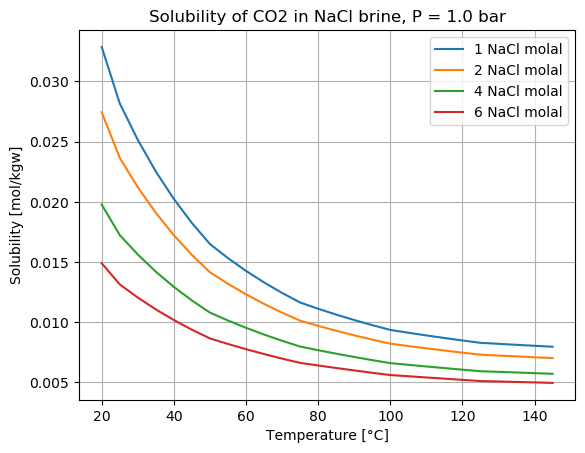
\includegraphics[height=0.37\columnwidth]{figures/intro/co2-solubility-nacl-h2o-1bar.png}
%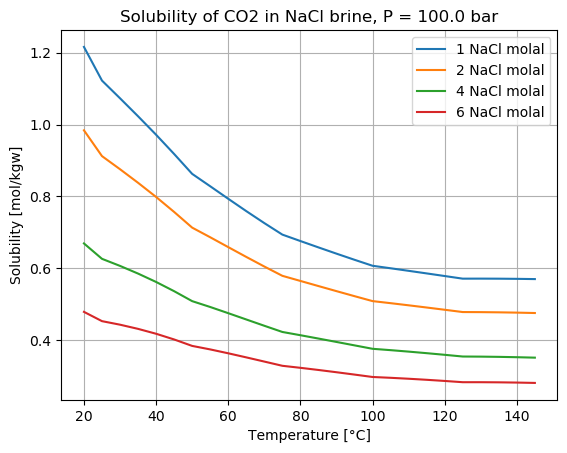
\includegraphics[height=0.3\columnwidth]{figures/intro/co2-solubility-nacl-h2o-100bar.png}\\
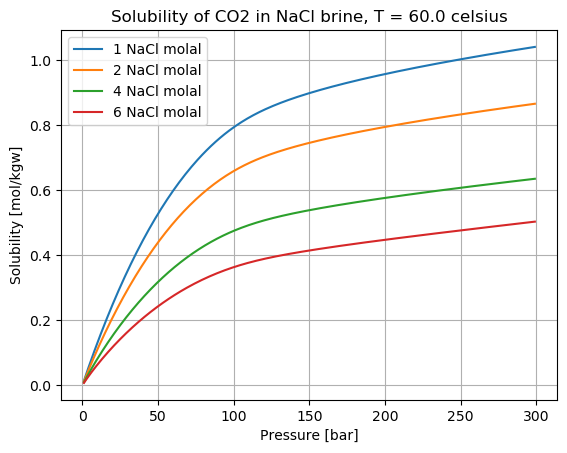
\includegraphics[height=0.37\columnwidth]{figures/intro/co2-solubility-nacl-h2o-vs-pressure-60celsius.png}
%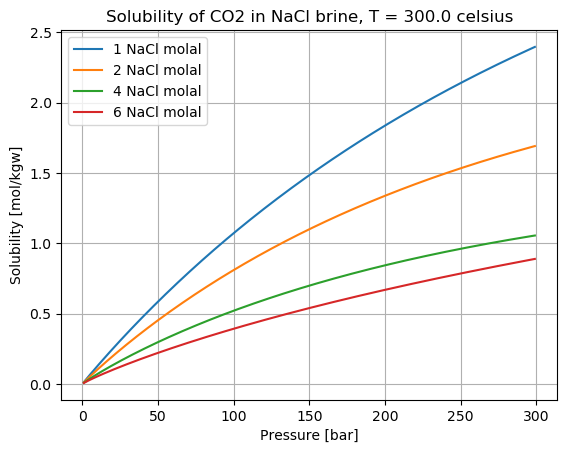
\includegraphics[height=0.3\columnwidth]{figures/intro/co2-solubility-nacl-h2o-vs-pressure-300celsius.png}
\end{figure}
}
\vskip 10pt
{\bf Note}: See Reaktoro v1 Jupyter notebook tutorial \href{https://github.com/mtsveta/reaktoro-jupyter/blob/geofluids-examples/tutorial/eq.co2-solubility-in-nacl-brine.ipynb}{\textcolor{indigo(dye)}{\it CO$_2$ solubility in NaCl-brine}} and \href{https://reaktoro.org/applications/solubility/solubility-co2-on-salinity-and-temperature.html}{\textcolor{indigo(dye)}{\it Reaktoro v2.0 example}} with the \href{https://github.com/mtsveta/reaktoro-v2-workshop/blob/main/tutorials/applications/salting-out-effect-co2.ipynb}{\textcolor{indigo(dye)}{\it Jupyter notebook}}.

\end{frame}

% --------------------------------------------------------------------------------------------------------------------%
% Learning Python
% --------------------------------------------------------------------------------------------------------------------%

\begin{frame}{Poll on the Python background}
\centering 
\vskip 10pt
{\Large \href{http://etc.ch/M2Rp}{\textcolor{indigo(dye)}{\tt http://etc.ch/M2Rp}}}\\ 
or \\[10pt]

\includegraphics[height=0.4\columnwidth]{figures/intro/poll.png}
\end{frame}

% --------------------------------------------------------------------------------------------------------------------%
% Learning Git
% --------------------------------------------------------------------------------------------------------------------%

\begin{frame}{Poll on the Git background}
\centering 
\vskip 10pt
{\Large \href{http://etc.ch/M2Rp}{\textcolor{indigo(dye)}{\tt http://etc.ch/M2Rp}}}\\ 
or \\[10pt]

\includegraphics[height=0.4\columnwidth]{figures/intro/poll.png}
\end{frame}

% --------------------------------------------------------------------------------------------------------------------%
% Learning Python
% --------------------------------------------------------------------------------------------------------------------%
\begin{frame}{Tips for learning Python}
\begin{itemize}
\item It is sufficient to learn the \alert{\textbf{basics of the Python 3}} using
\end{itemize}
\begin{center}
{\href{https://www.programiz.com/python-programming/tutorial}{\textcolor{indigo(dye)}{\tt https://www.programiz.com/python-programming/tutorial}}}{\large\par}
\par\end{center}
\begin{itemize}
\item \alert{\textbf{Git}} intro
\end{itemize}
\begin{center}
{\href{https://youtu.be/hwP7WQkmECE}{\textcolor{indigo(dye)}{\tt https://youtu.be/hwP7WQkmECE}}}{\large\par}
\par\end{center}
\begin{itemize}
\item Consider installing Python 3 using \alert{\textbf{Anaconda}} using
\end{itemize}
\begin{center}
{\href{https://www.anaconda.com/distribution/}{\textcolor{indigo(dye)}{\tt https://www.anaconda.com/distribution/}}}{\large\par}
\par\end{center}
\begin{itemize}
\item Instruction of \alert{\textbf{installing Reaktoro}} are also given using Anaconda are given in videos 
\emph{Intro words}, 
\emph{Installation on Windows / IoS}, and 
\emph{Reaktoro Jyputer Notebook Installation} with explanation on Reaktoro installation and Jupyter Notebook tutorials execution are available \href{https://polybox.ethz.ch/index.php/s/qStBnxUnry648U5}{\textcolor{indigo(dye)}{\tt here}}. 
%
\item 
Questions are always welcome via my email \href{svetlana.kyas@erdw.ethz.ch}{\textcolor{indigo(dye)}{\tt svetlana.kyas@erdw.ethz.ch}}. 
%or the \href{https://gitter.im/geofluids/community}{\textcolor{indigo(dye)}{\it Gitter chat}} (requires the github account).
\end{itemize}

\end{frame}
% --------------------------------------------------------------------------------------------------------------------%
% A brief overview of geochemical modeling and its applications
% --------------------------------------------------------------------------------------------------------------------%
%
\subsection{A brief overview of geochemical modeling and its applications}
%
\begin{frame}{What is geochemical modeling?}
\vskip 10pt
 \textbf{Geochemical modeling} is the use of computers to simulate \textbf{chemical
reactions} occurring in geologic systems, either \textbf{near the
Earth's surface} or \textbf{deep in its interior}.
%
\lcol
\begin{singlespace}
%
\begin{figure}
\centering
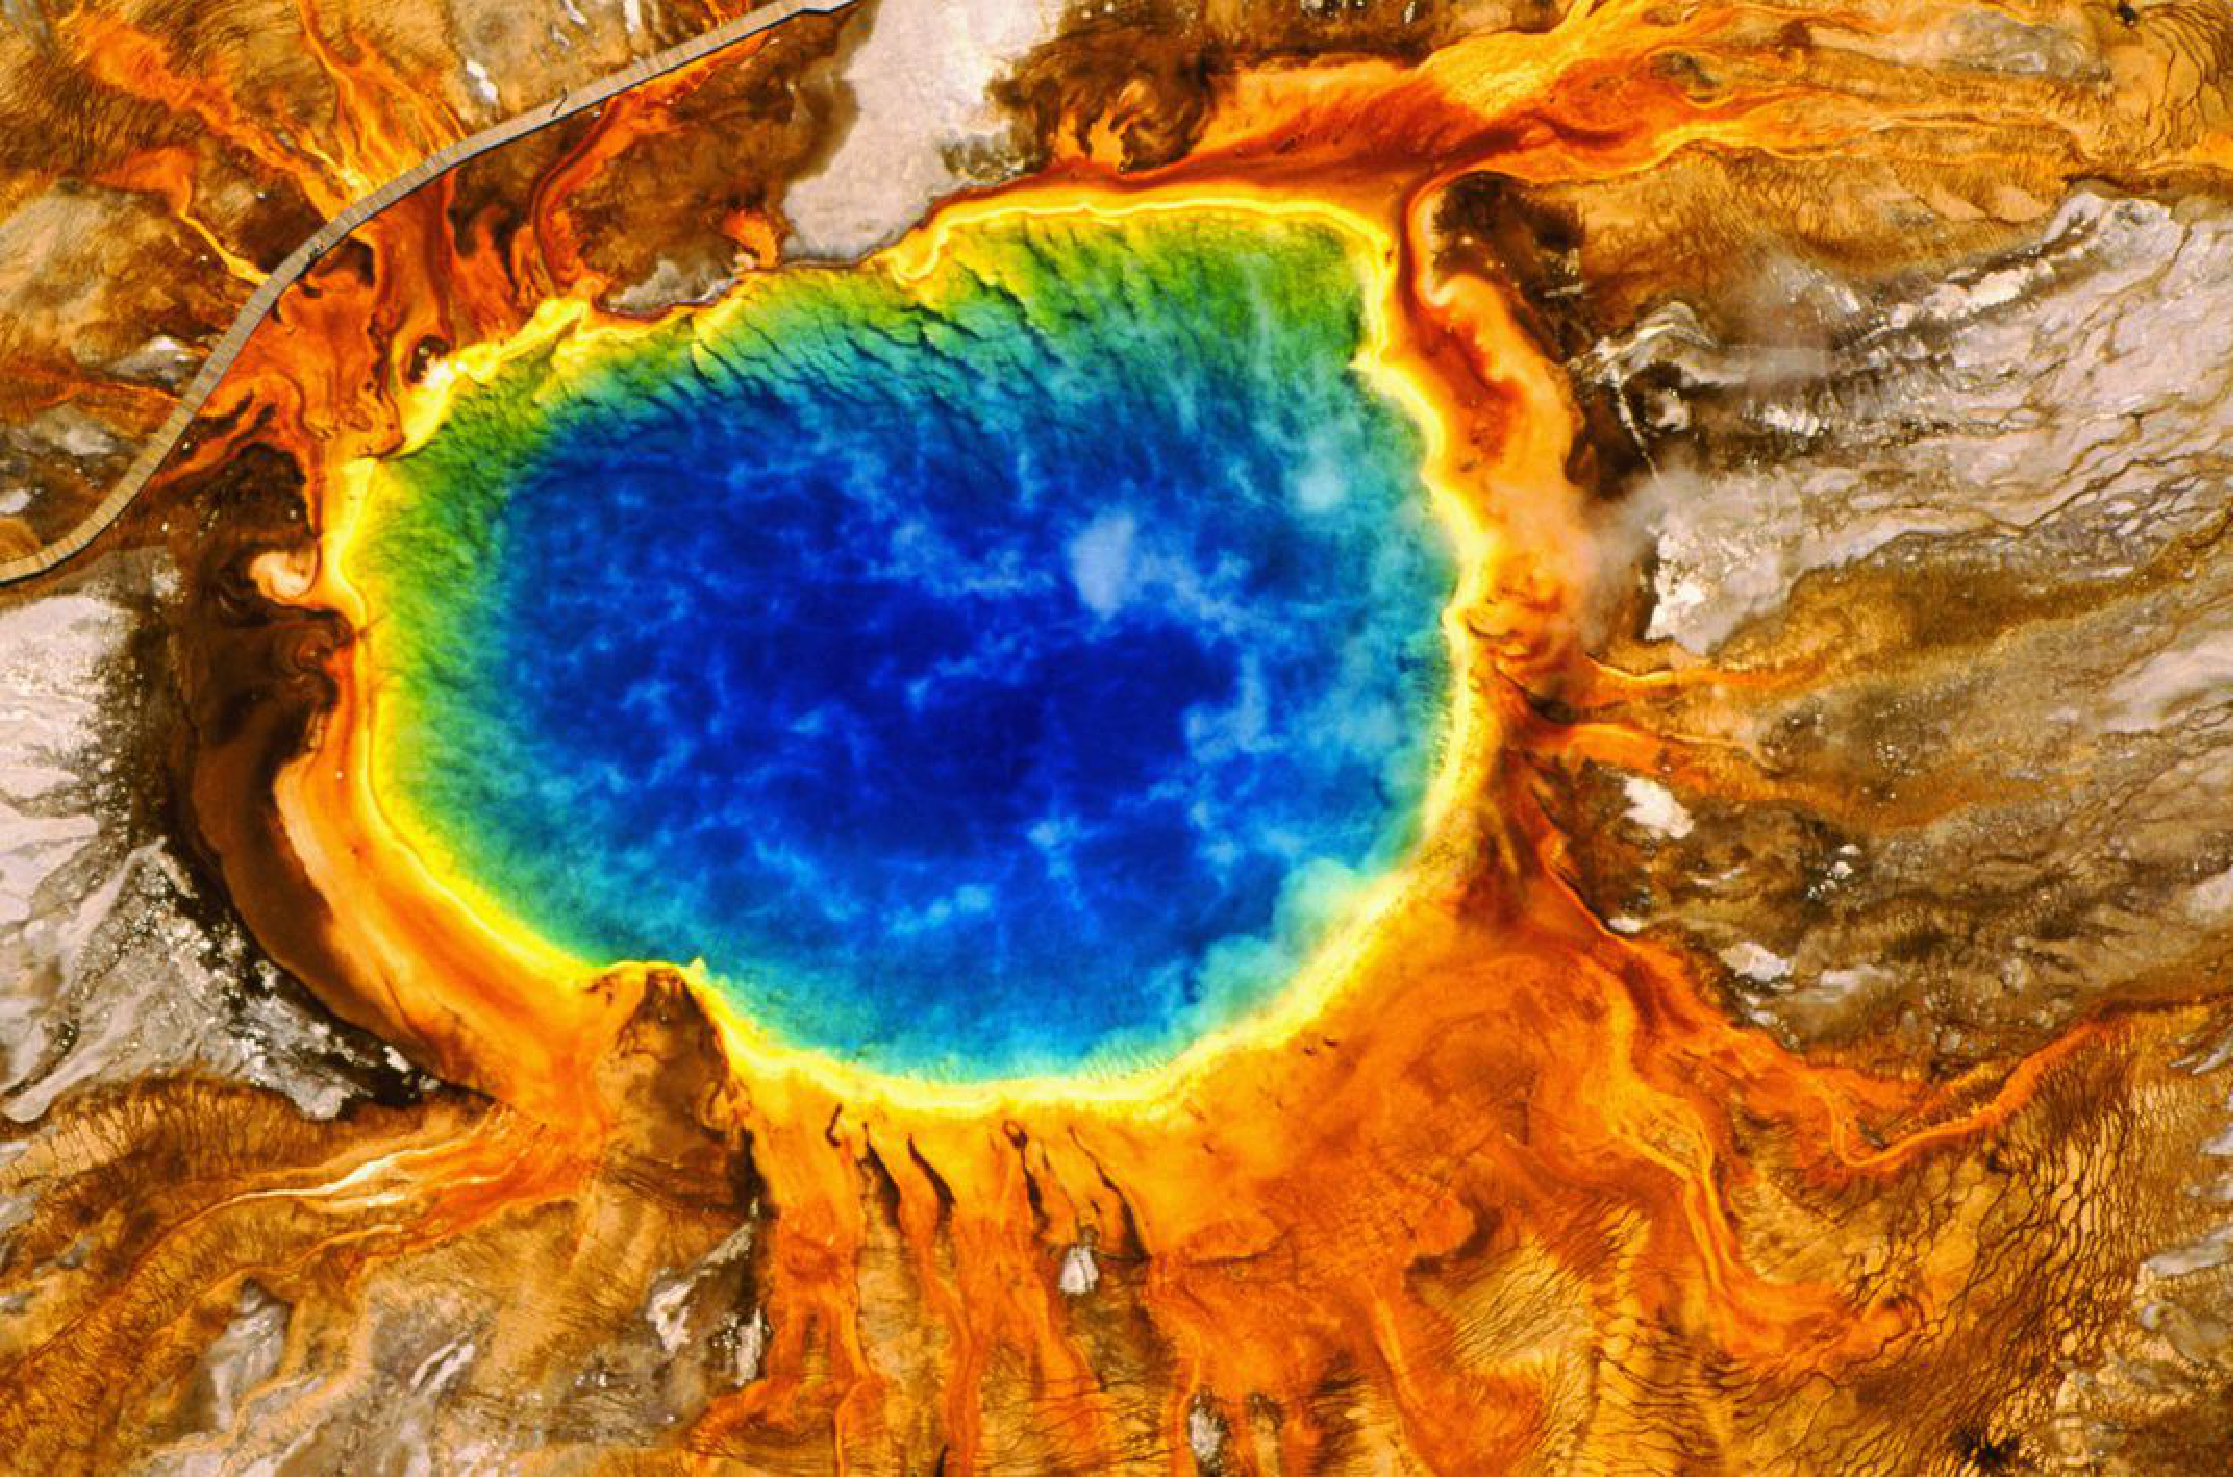
\includegraphics[height=0.5\columnwidth]{figures/applications/example-of-geochemical-reactions-in-yellowstone-geysers}
\caption*{Geochemical reaction calculations for thermal water analysis 
(Grand Prismatic, Midway Geyser Basin, Yellowstone, Wyoming, USA).}
\end{figure}
%
\end{singlespace}
%
\rcol
\begin{figure}
\vskip 5pt
\centering
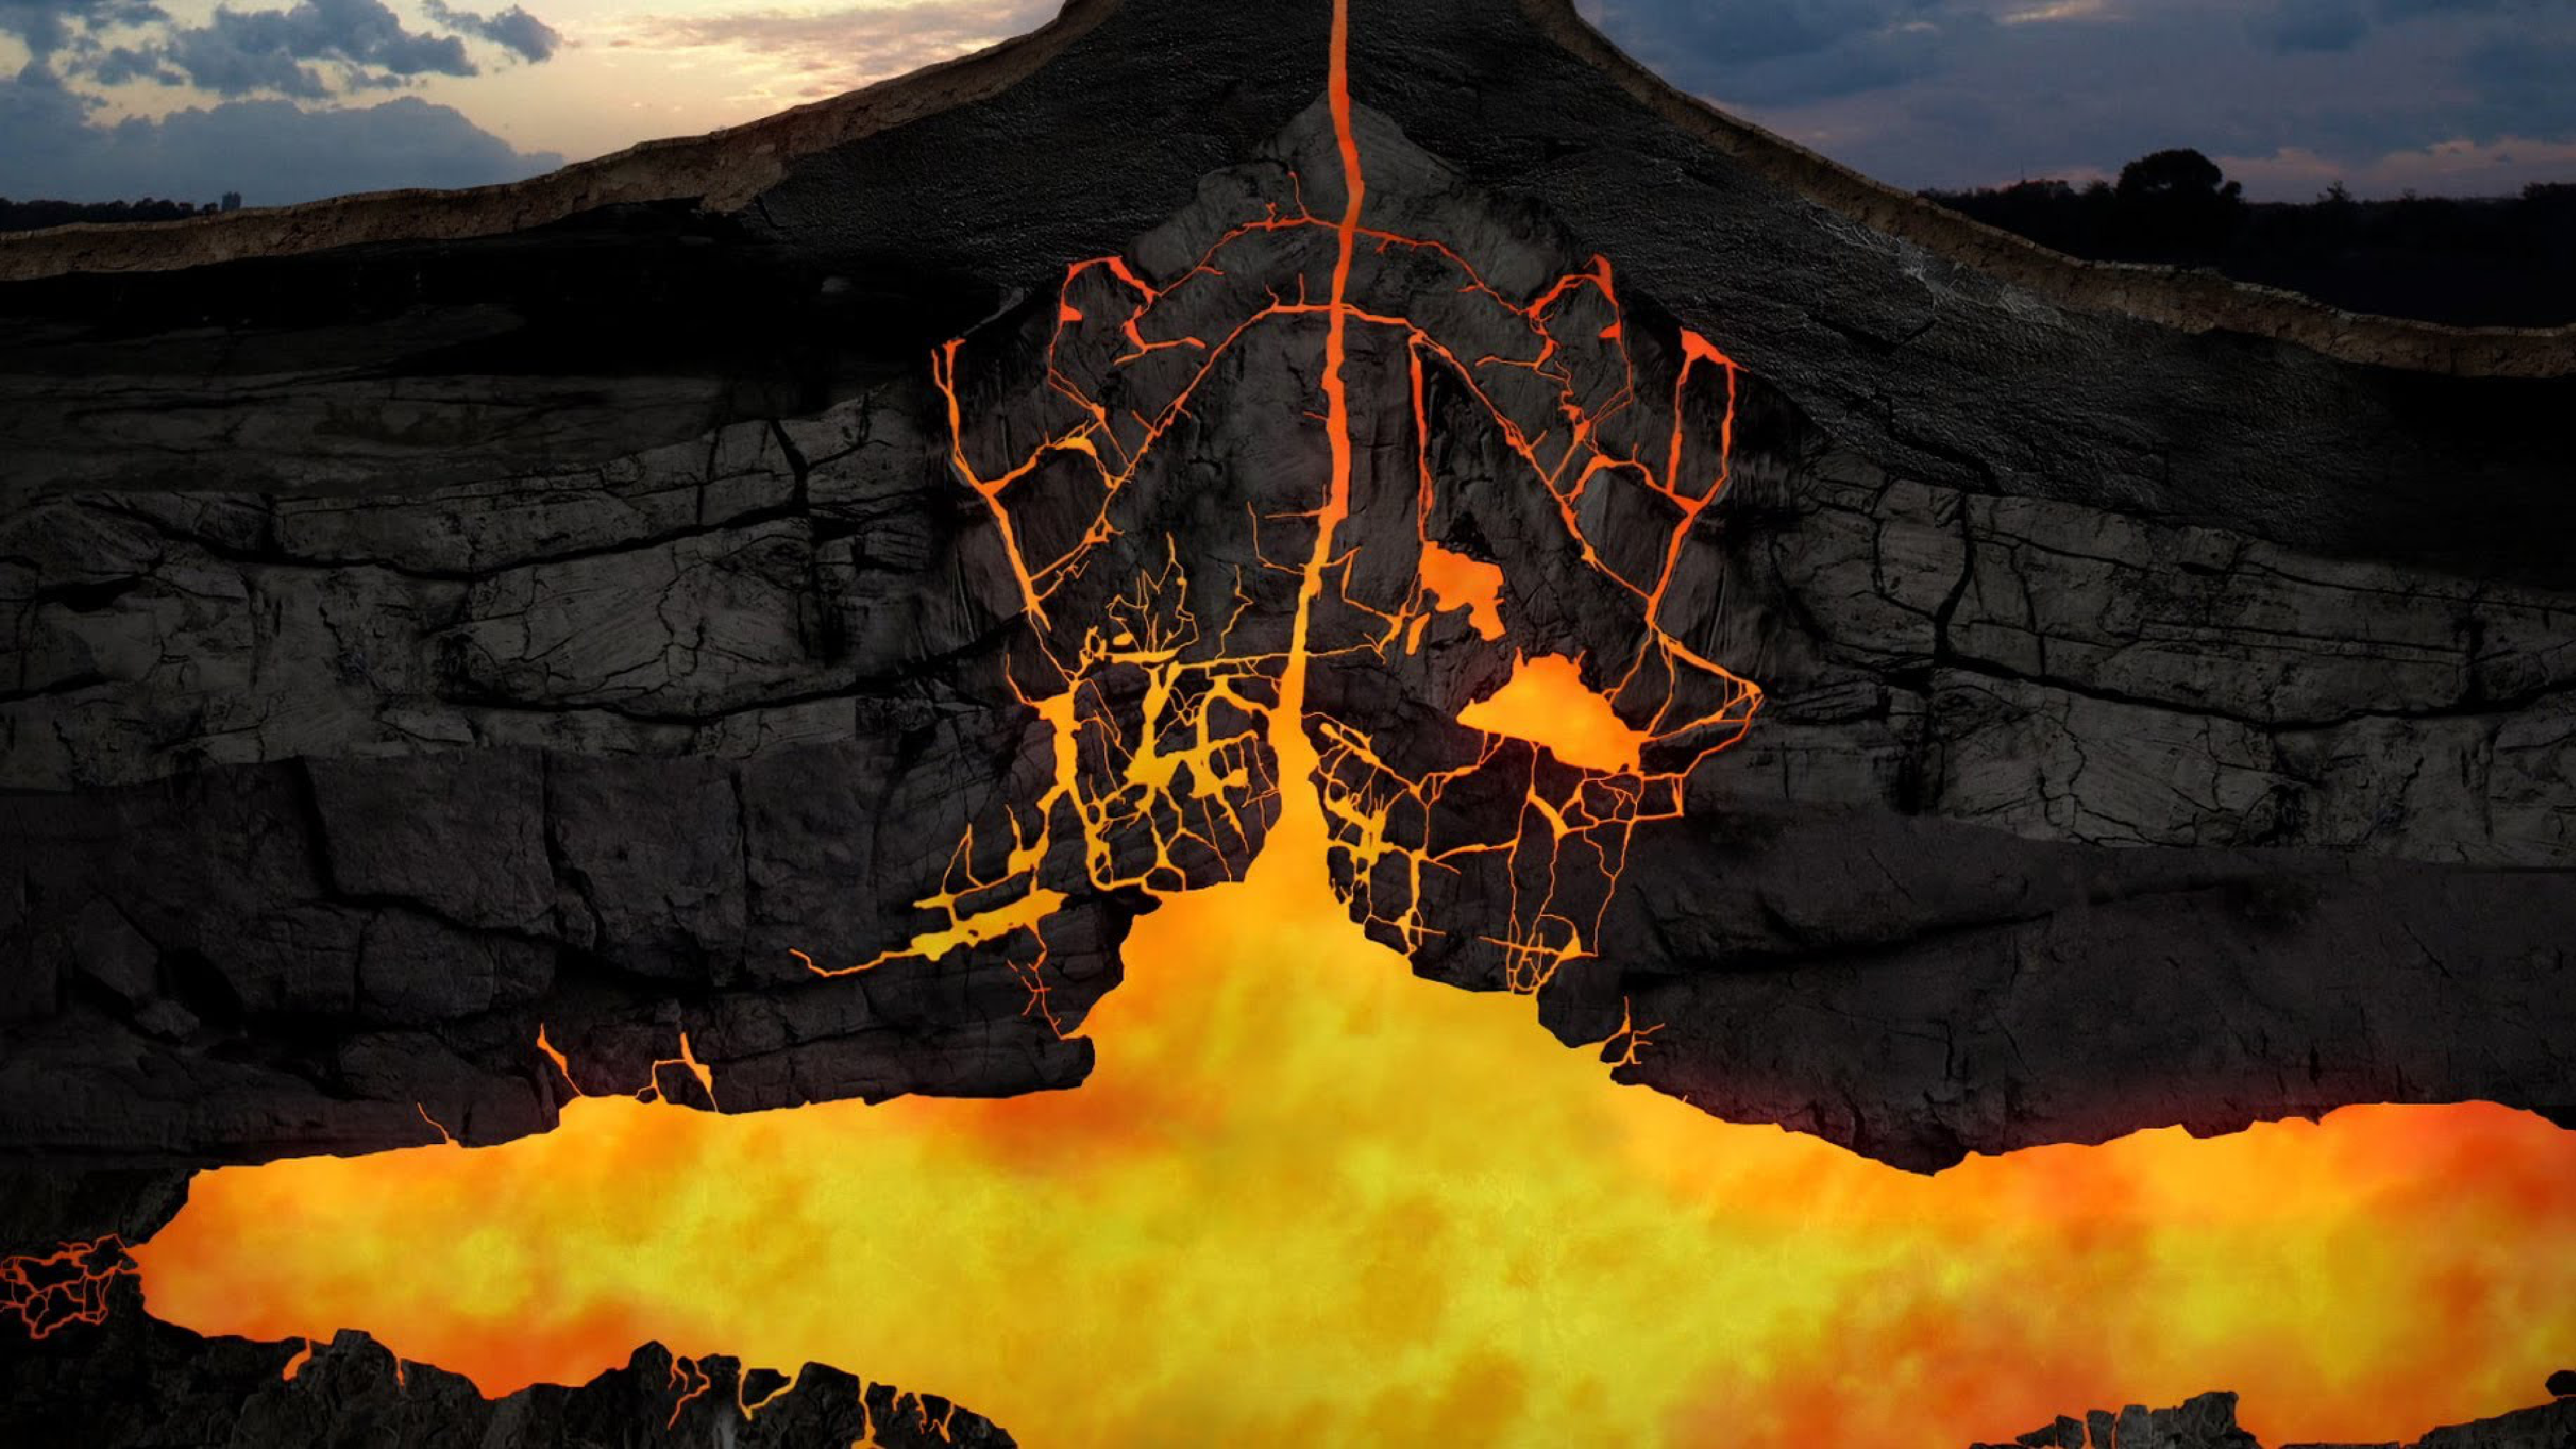
\includegraphics[height=0.5\columnwidth]{figures/applications/example-of-geochemical-reactions-in-a-volcano-magma-chamber}
\caption*{Geochemical reaction calculations for molten rocks as the magma flows
from the Earth's mantle upwards.}
\end{figure}
\ecol
\end{frame}

% --------------------------------------------------------------------------------------------------------------------%
% Geochemical modeling applications, Scaling prediction in wells
% --------------------------------------------------------------------------------------------------------------------%
%
\begin{frame}{Geochemical modeling applications, Scaling prediction in wells}
%
\lcol
%
\vskip 20pt
\begin{figure}
\centering
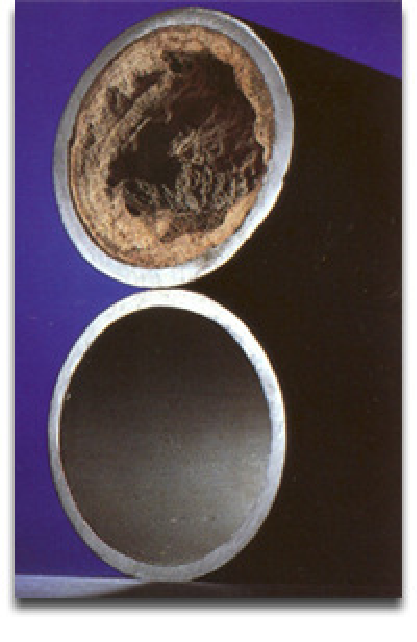
\includegraphics[height=0.6\textheight]{figures/applications/scaling-calcium-strontium-barium}
\caption*{Scale formation in a well as a result of geochemical reactions leading
to mineral precipitation.}
\end{figure}
%
\rcol
\vskip -20pt
\begin{itemize}[<+->]
\item Fluids coming from a reservoir experiences \textbf{temperature\slash pressure
changes along the wells}.
\item The decrease in temperature and/or pressure can lead to chemical reactions 
promoting precipitation of minerals and thus \textbf{scale formation} along the well.
\item Geochemical modeling can be used to \textbf{predict}, \textbf{understand},
and \textbf{assist }on the \textbf{\alert{\textbf{remediation of scale formation}}}.
\end{itemize}
\ecol
%
\end{frame}

% --------------------------------------------------------------------------------------------------------------------%
% Geochemical modeling applications: CO$_{\boldsymbol{2}}$ storage
% in geologic formations
% --------------------------------------------------------------------------------------------------------------------%
%
\begin{frame}{Geochemical modeling applications, 
CO$_{\boldsymbol{2}}$ storage in geologic formations}
%
\vskip 10pt
\lcol
%
\begin{figure}
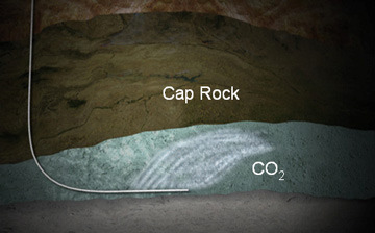
\includegraphics[height=3.8cm]{figures/applications/co2-storage-injection}
\caption*{Once CO$_{2}$ is injected in a deep saline aquifer, it starts to
\textbf{dissolve into the resident brine}. Geochemical calculations
can be used to calculate how much CO$_{2}$ dissolves and how much
CO$_{2}$ continues mobile as gas or supercritical fluid.}
\end{figure}
%
\rcol
%
\begin{figure}
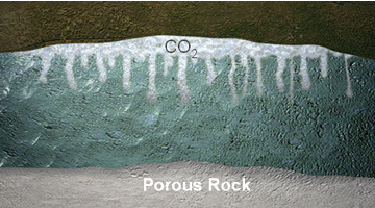
\includegraphics[height=3.8cm]{figures/applications/co2-storage-fingers}
\caption*{Brine with dissolved CO$_{2}$ becomes acidic. It can then more easily 
\textbf{react with rock minerals}. This change rock properties, such as \textbf{porosity} 
and \textbf{permeability}. Geochemical calculations can tell {\bf how much rock 
minerals dissolve}.}
\end{figure}
%
\ecol
%
\end{frame}
%
% --------------------------------------------------------------------------------------------------------------------%
% Geochemical modeling applications: Water analysis
% --------------------------------------------------------------------------------------------------------------------%
%
\begin{frame}{Geochemical modeling applications, Water analysis}
%
Given the following water analysis, with the concentration of many chemical elements and 
pH, \textbf{find the concentrations of all aqueous species in the water}:
\lcol
\begin{figure}
\centering
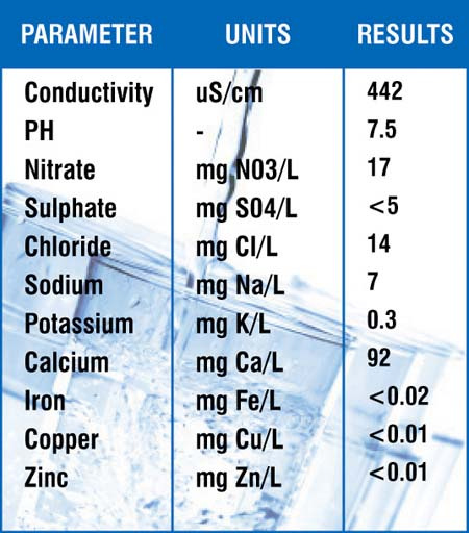
\includegraphics[height=0.6\textheight]{figures/applications/water-analysis}
\caption*{Water composition as a result of a water analysis.}
\end{figure}
\rcol
%
\begin{figure}
\centering
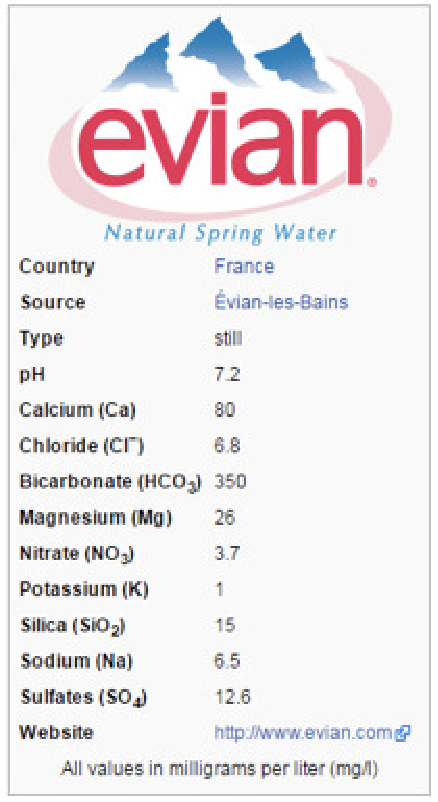
\includegraphics[height=0.6\textheight]{figures/applications/evian-chemical-water-composition}
\caption*{See Jupyter notebook tutorial \href{https://github.com/mtsveta/reaktoro-v2-workshop/blob/main/tutorials/applications/evian-water-analysis.ipynb}{\textcolor{indigo(dye)}{\it Analysis of the Evian water}}.}
\end{figure}
%
\ecol
%
\end{frame}

% --------------------------------------------------------------------------------------------------------------------%
% Geochemical modeling applications: Water analysis, Part II
% --------------------------------------------------------------------------------------------------------------------%
%
\begin{frame}{Geochemical modeling applications: Water analysis}
\textbf{Selected aqueous species} that could exist in that water sample:
\vskip 1pt
{\scriptsize%
\begin{tabular*}{1\columnwidth}{@{\extracolsep{\fill}}ccccccc}
Cl-(aq) & CuO(aq) & H2(aq) & HNO2(aq) & KSO4-(aq) & OH-(aq) & SO3-{}-(aq)
\tabularnewline
ClO-(aq) & CuO2-{}-(aq) & H2N2O2(aq) & HNO3(aq) & N2(aq) & S2-{}-(aq) & SO4-{}-(aq)\tabularnewline
ClO2-(aq) & CuOH+(aq) & H2O(aq) & HO2-(aq) & N2H5+(aq) & S2O3-{}-(aq) & Zn++(aq)\tabularnewline
ClO3-(aq) & Fe++(aq) & H2O2(aq) & HS-(aq) & N2H6++(aq) & S2O4-{}-(aq) & ZnCl+(aq)\tabularnewline
ClO4-(aq) & Fe+++(aq) & H2S(aq) & HS2O3-(aq) & N2O2-{}-(aq) & S2O5-{}-(aq) & ZnCl2(aq)\tabularnewline
Cu+(aq) & FeCl+(aq) & H2S2O3(aq) & HS2O4-(aq) & NH3(aq) & S2O6-{}-(aq) & ZnCl3-(aq)\tabularnewline
Cu++(aq) & FeCl++(aq) & H2S2O4(aq) & HSO3-(aq) & NH4+(aq) & S2O8-{}-(aq) & ZnO(aq)\tabularnewline
CuCl(aq) & FeCl2(aq) & HCl(aq) & HSO4-(aq) & NO2-(aq) & S3-{}-(aq) & ZnO2-{}-(aq)\tabularnewline
CuCl+(aq) & FeO(aq) & HClO(aq) & HSO5-(aq) & NO3-(aq) & S3O6-{}-(aq) & ZnOH+(aq)\tabularnewline
CuCl2(aq) & FeO+(aq) & HClO2(aq) & HZnO2-(aq) & Na+(aq) & S4-{}-(aq) & \tabularnewline
CuCl2-(aq) & FeO2-(aq) & HCuO2-(aq) & K+(aq) & NaCl(aq) & S4O6-{}-(aq) & \tabularnewline
CuCl3-(aq) & FeOH+(aq) & HFeO2(aq) & KCl(aq) & NaOH(aq) & S5-{}-(aq) & \tabularnewline
CuCl3-{}-(aq) & FeOH++(aq) & HFeO2-(aq) & KHSO4(aq) & NaSO4-(aq) & S5O6-{}-(aq) & \tabularnewline
CuCl4-{}-(aq) & H+(aq) & HN2O2-(aq) & KOH(aq) & O2(aq) & SO2(aq) & \tabularnewline
\end{tabular*}}

\pause
\vskip 5pt
\alert{\textbf{Questions}} we want to answer: 
\begin{itemize}
\item What are the \textbf{amounts of these species}? 
\item How \textbf{saturated} is the water \textbf{with respect to several minerals}? \\
\textbf{Note:}  \emph{saturation} is the tendency of the solution to dissolve/precipitate a mineral.
\end{itemize}
\end{frame}
%
% --------------------------------------------------------------------------------------------------------------------%
% Other applications for geochemical modeling
% --------------------------------------------------------------------------------------------------------------------%
%
\begin{frame}{Other applications for geochemical modeling}
\begin{itemize}
\item Geochemical reaction calculations can be used for a wide range of
\textbf{industrial and environmental applications}: 
\begin{itemize}
\item nuclear waste management to ensure radionuclides remain properly stored
for thousands\slash millions of years;
\item ore-forming processes;
\item geochemical reactions in geothermal and hydrothermal systems;
\item enhanced oil and gas recovery (prediction of gas and mineral solubility 
at the wide range of temperatures and pressures);
\item transport of reactive solution in porous and fractured media.
\end{itemize}
\end{itemize}

\begin{figure}
\centering
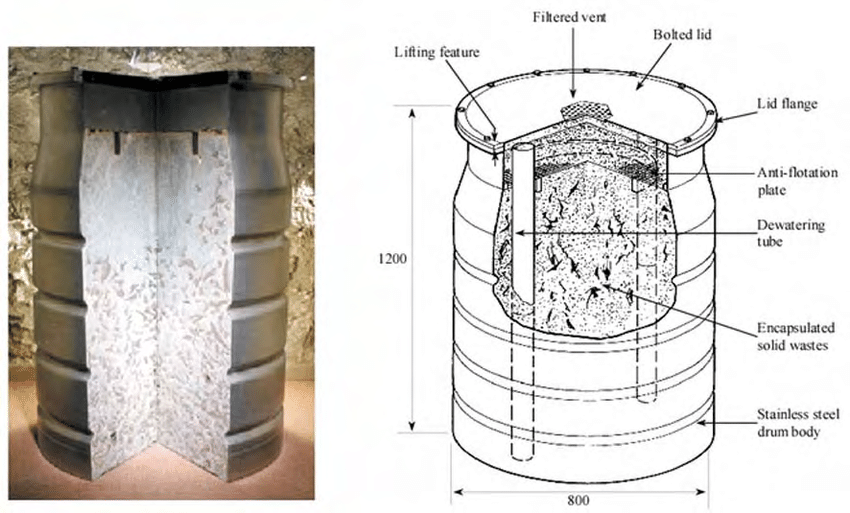
\includegraphics[height=0.2\columnwidth]{figures/applications/waste-storage.png} \quad %\caption*{Radioactive waste captured in cement.}
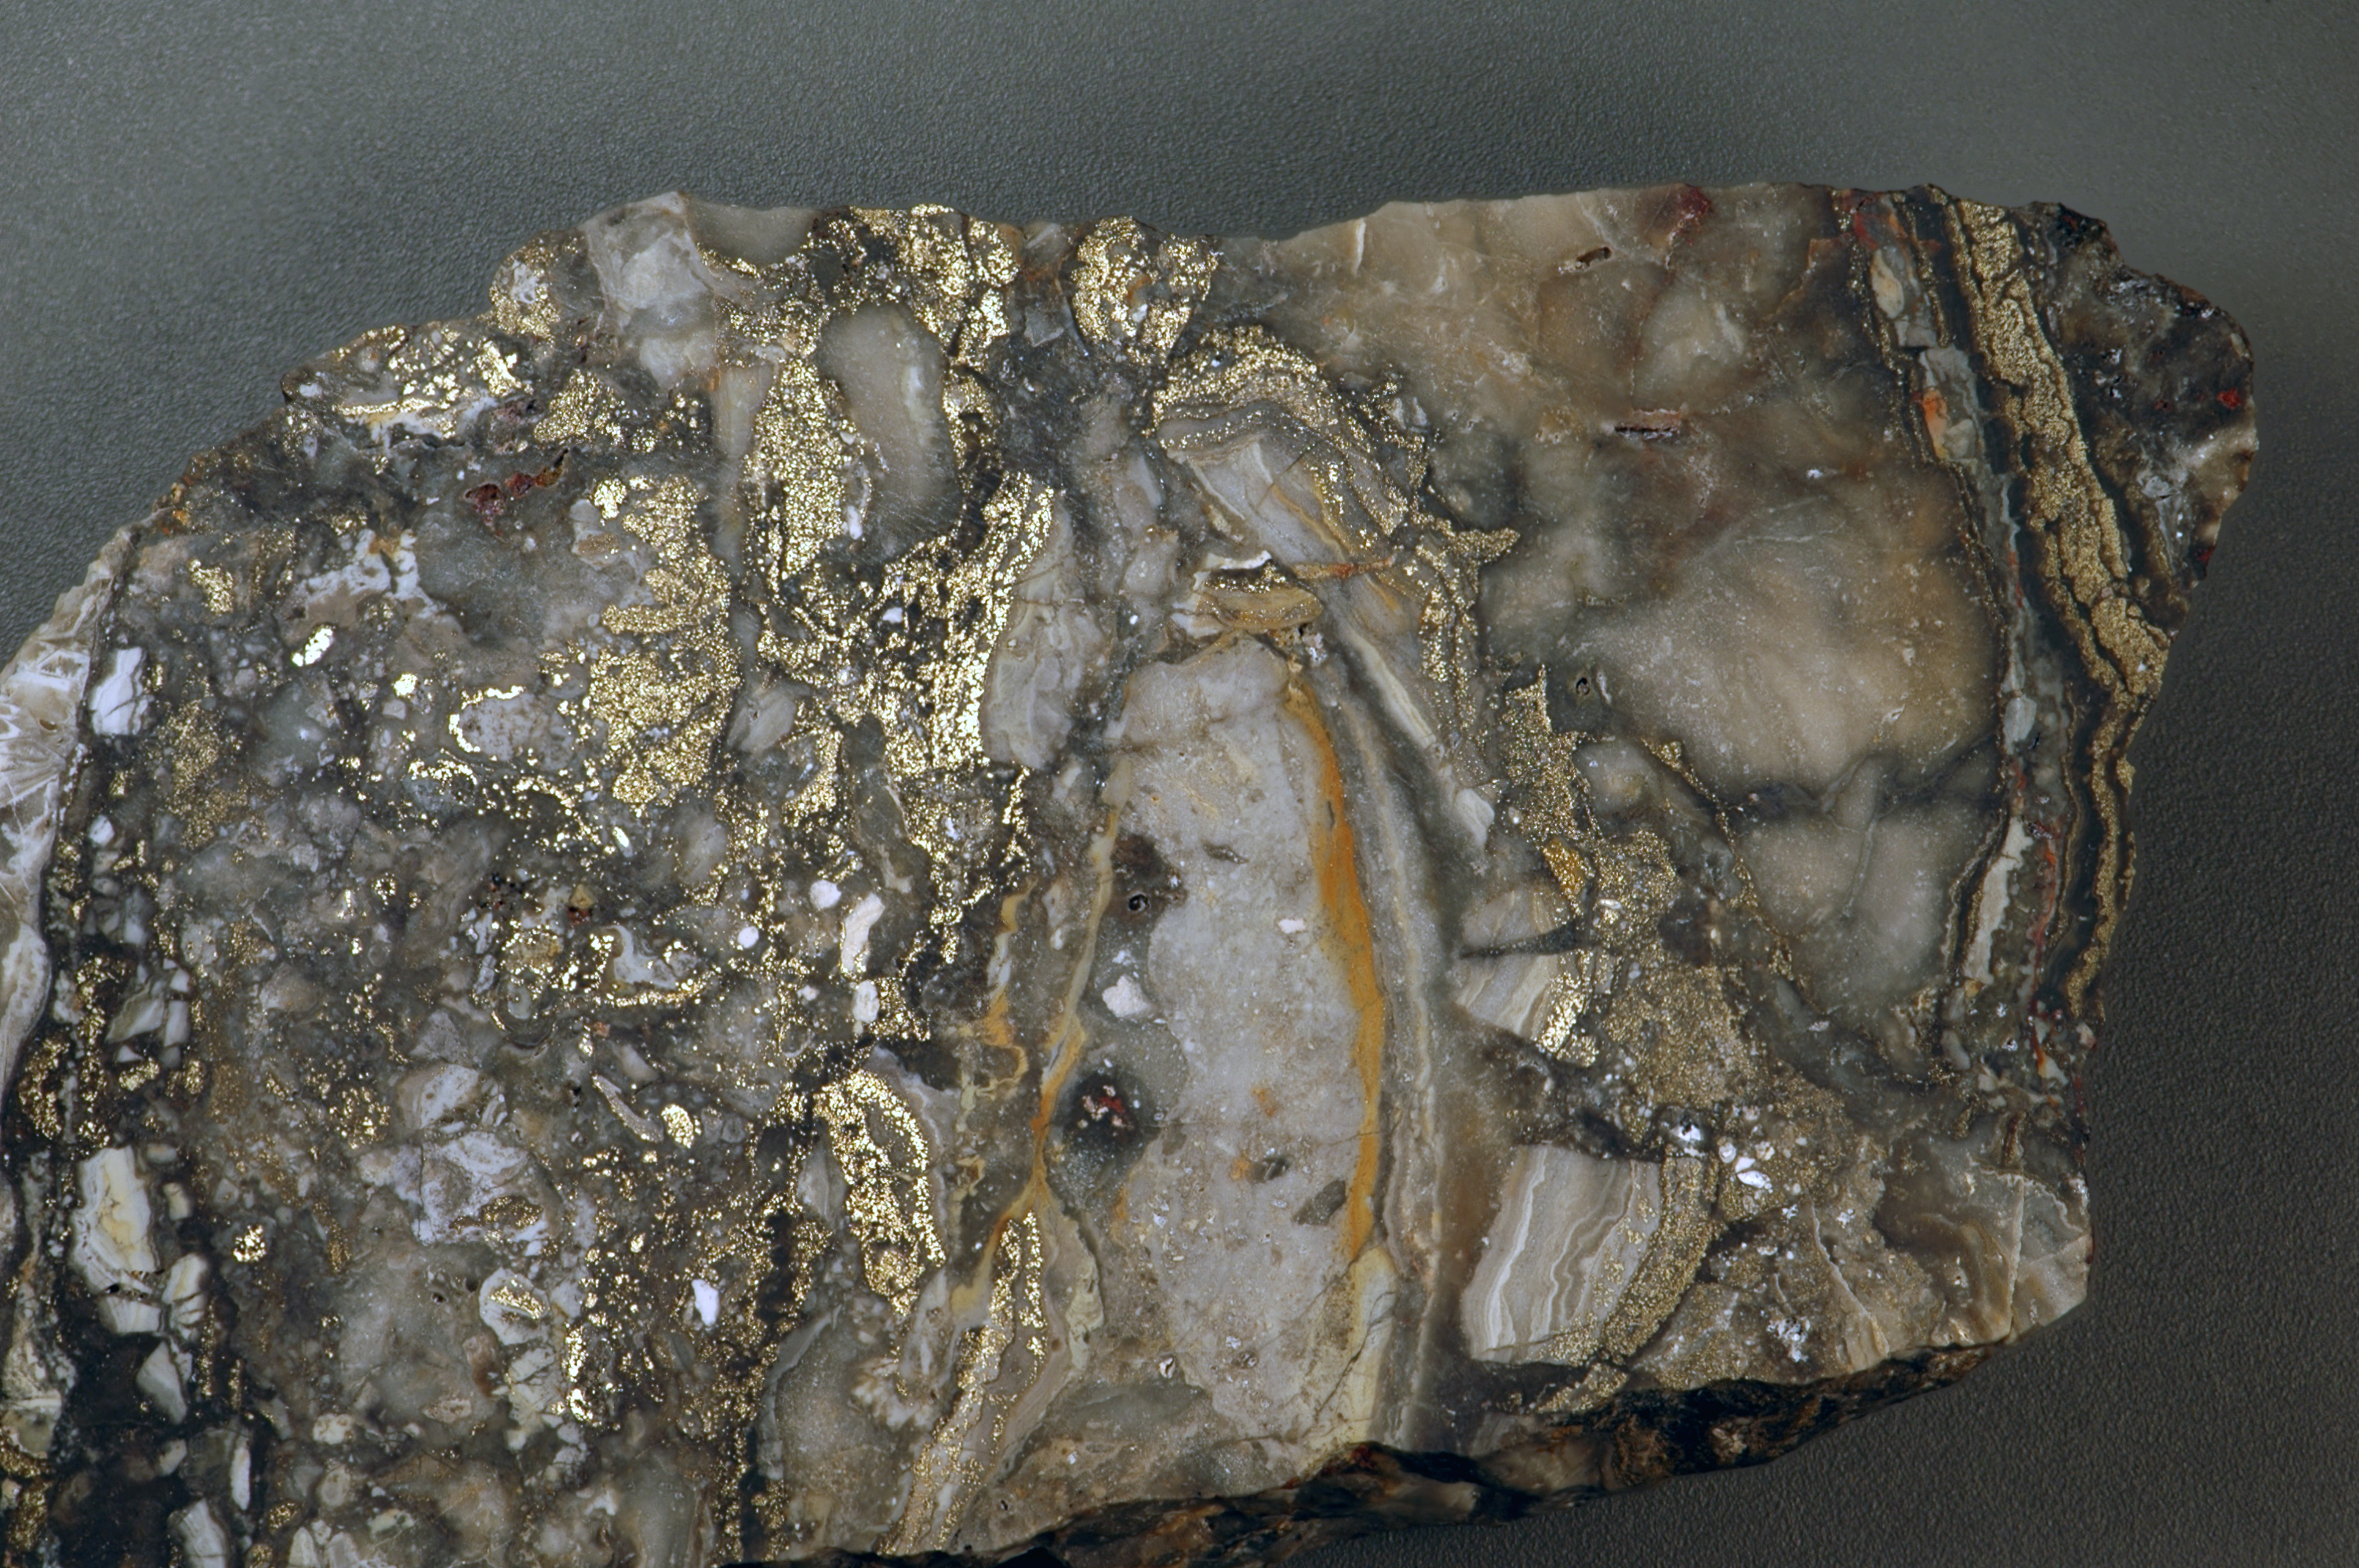
\includegraphics[height=0.2\columnwidth]{figures/applications/ore-forming.jpg}  \quad %\caption*{Ore forming processes.}
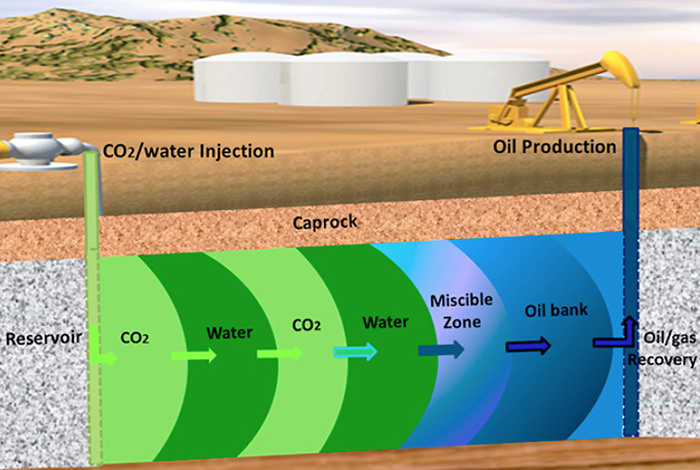
\includegraphics[height=0.2\columnwidth]{figures/applications/enhanced-oil-recovery.jpg}%\caption*{Enhanced oil and gas recovery.}
\end{figure}

\end{frame}

\subsection{Chemical equilibrium and chemical kinetics for modeling geochemical
systems}

% --------------------------------------------------------------------------------------------------------------------%
% Intuition about chemical reaction behavior
% --------------------------------------------------------------------------------------------------------------------%

\begin{frame}{Chemical reaction behavior,  Initial intuition}
	\vskip 5pt
\begin{itemize}
\item Consider 1 kg of H$_{2}$O mixed with 1 mg of NaCl (halite). 
\pause
\item Chemical reactions that occur among the species in the solution and the halite are as follows:\\[-30pt]
\begin{align*}
\mathsf{NaCl(halite, s)} & \rightleftharpoons\mathsf{Na^{+}+Cl^{-}}\\
\mathsf{Na^{+}+Cl^{-}} & \rightleftharpoons\mathsf{NaCl(aq)}\\
\mathsf{H_{2}O} & \rightleftharpoons\mathsf{H^{+}+OH^{-}}
\end{align*}
\vskip -5pt
\pause
\item Detailed steps: 
\begin{itemize}
\item \textbf{pure water} solution contains species: H$_2$O, H$^+$, OH$^-$, O$_2$(aq), H$_2$(aq)
\item \textbf{scale of the species} in water solution: 
55.508 mol of H$_2$O, 1e-7 mol of H$^+$, 1e-7 mol of OH$^-$ (to make sure the charge balance),
 1e-31 mol of O$_2$(aq),  1e-31 mol of H$_2$(aq) 
\item after \textbf{mixing} NaCl(s) we have in addition: Na$^{+}$, Cl$^{-}$, NaCl(aq), HCl(aq), NaOH(aq)
\item  \textbf{new ions} H$^+$ and Cl$^{-}$ produce $\mathsf{H^{+}+Cl^{-}} \rightleftharpoons \mathsf{HCl(aq)}$
\end{itemize}
\pause
\item What can we say about the \alert{\textbf{behavior and time-scale}} of the these species after 1 ms, 1 s, 1 min?
\end{itemize}
\end{frame}
%
% --------------------------------------------------------------------------------------------------------------------%
% Reaction classification
% --------------------------------------------------------------------------------------------------------------------%
%
\begin{frame}{Reaction classification}
	\begin{itemize}
		\item \alert{\bf Irreversible} or \alert{\bf reversible}:
		\begin{itemize}
			\item An {\bf irreversible} reaction is one that occurs in only one direction and continues in this direction until at least one of the reactants is depleted.
			\item A {\bf reversible} reaction can occur in both directions (with forward and backward reaction reaction coefficients $k_f$ and $k_b$, respectively):
			%
			\[	
			\mathsf{a\,A + b\,B} \xrightleftharpoons[k_b]{k_f} \mathsf{c\,C + d\,D}.
			%\quad 
			%\mbox{with equilibrium constant}
			\quad
			%K_e := \tfrac{k_f}{k_b} = \tfrac{\mathsf{[C]^c\, [D]^d}}{\mathsf{[A]^a\,[B]^b}}.
			\]
			%
		\end{itemize}
		%%%
		\item \alert{\bf Homogeneous} or \alert{\bf heterogeneous}:
		\begin{itemize}
			\item A {\bf homogeneous} reaction involves a single phase, e.g., 
			%
			\begin{alignat*}{2}
				\mbox{Formation of ammonia}:  \mathsf{N_2(g) + 3\,H_2(g) } & \mathsf{\xrightleftharpoons[]{} 2\,NH_3(g)}\\
				\mbox{Oxidation of sulfur dioxide}: \mathsf{2\,SO_2(g) + O_2(g) } & \mathsf{\xrightleftharpoons[]{} 2\,SO_3(g)} 
			\end{alignat*}
			%
			\item A {\bf heterogeneous} reaction involves more than one phase, e.g., 
			\begin{alignat*}{2}
				\mbox{Carbonation} : \mathsf{Ca(OH)_2(s) + CO_2(g)} & \mathsf{\xrightleftharpoons[]{} CaCO_3(s) + H_2O(l)}
			\end{alignat*}
		\end{itemize}
		
	\end{itemize}
\end{frame}
%
% --------------------------------------------------------------------------------------------------------------------%
% Chemical kinetics vs. chemical equilibrium
% --------------------------------------------------------------------------------------------------------------------%

\begin{frame}{Chemical kinetics vs. Chemical equilibrium}
%
\small
\lcol
\vskip 10pt
\begin{cbox}{Chemical Kinetics}
$\bullet$ Focuses on \alert{\textbf{pathways of reactions}} and  \alert{\textbf{its rate}}. \\
$\bullet$ Used to compute the amounts of the reacting species \alert{\textbf{over time}}. \\
\end{cbox}

\begin{cbox}{Chemical Equilibrium} 
$\bullet$ Focuses on the reactions with \alert{\textbf{net rates are zero}}. \\
$\bullet$ Used to directly compute the final composition of the species when
the reactions are \alert{\textbf{in equilibrium}}. 
\end{cbox}

\rcol

\vskip 10pt
\begin{figure}
\centering
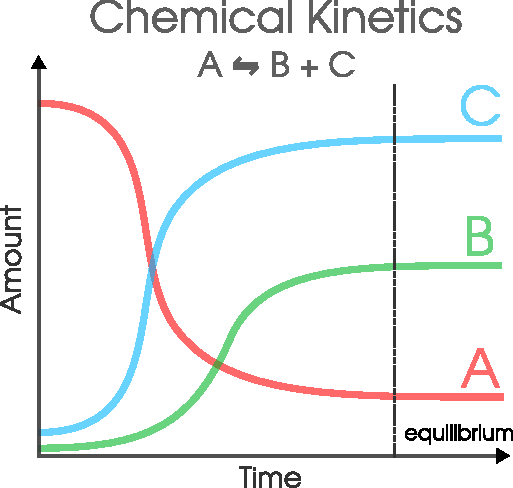
\includegraphics[width=0.8\columnwidth]{figures/applications/chemical-kinetics-equilibrium-illustration-evolution-plot}
\caption*{Chemical kinetics evolution of species A, B, and C over time.}
\end{figure}

\ecol

\end{frame}

% --------------------------------------------------------------------------------------------------------------------%
% Examples of chemical equilibrium reactions
% --------------------------------------------------------------------------------------------------------------------%

\begin{frame}{Examples of chemical equilibrium reactions}
%
\lcol

\begin{itemize}
	\item \alert{\textbf{Bottle with soda drink}}
	\begin{itemize}
		\item CO$_2$(g) dissolved in the liquid
		\item CO$_2$(g) is in the space between the liquid and the cap
		\item CO$_2$ is constantly moving from the liquid to the gas phase, and back
		\begin{align*}
			\mathsf{CO_2(g) + H2O(l)} & \rightleftharpoons \mathsf{H_2CO_3(aq)}
		\end{align*}
	\end{itemize}
%
	\pause
	\item \alert{\textbf{(Oxy)haemoglobin reactions in blood}}
	\begin{itemize}
		\item haemoglobin takes up oxygen and releases it
		\begin{align*}
			\mathsf{haemoglobin(aq) + 4 O_2(g) } & \rightleftharpoons 	
			\mathsf{haemoglobin(O_2)_4(aq)}
		\end{align*}
		\item oxyhaemoglobin goes through the blood stream to cells
	\end{itemize}
\end{itemize}      

\rcol

\begin{figure}
\centering
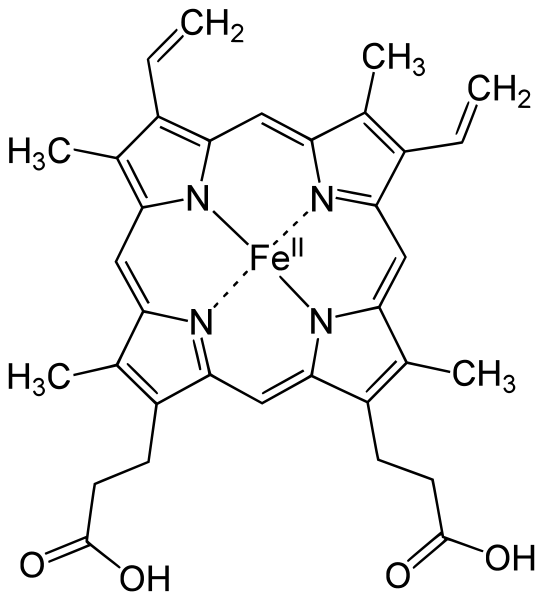
\includegraphics[width=0.8\columnwidth]{figures/applications/hemoglobin.png}
\caption*{Hemoglobin structure.}
\end{figure}

\ecol

\end{frame}

% --------------------------------------------------------------------------------------------------------------------%
% Examples of chemical kinetics reactions
% --------------------------------------------------------------------------------------------------------------------%

\begin{frame}{Examples of chemical kinetics reactions}
%
\lcol

\begin{itemize}
	\item \alert{\textbf{Corrosion}}, a natural process that converts a refined metal into a more chemically stable form such as oxide, hydroxide, or sulfide.
		\begin{itemize}
		\item galvanic corrosion 
		\item electrolytic corrosion
		\item microbial corrosion
		\item high temperature corrosion
	\end{itemize}
	%
	\pause
	\item \alert{\textbf{Fluid catalytic cracking (FCC)}}, a conversion process of petroleum crude oils into gasoline, olefinic gases, and other products. Used in petroleum refineries.
\end{itemize}      

\rcol

\begin{figure}
\centering
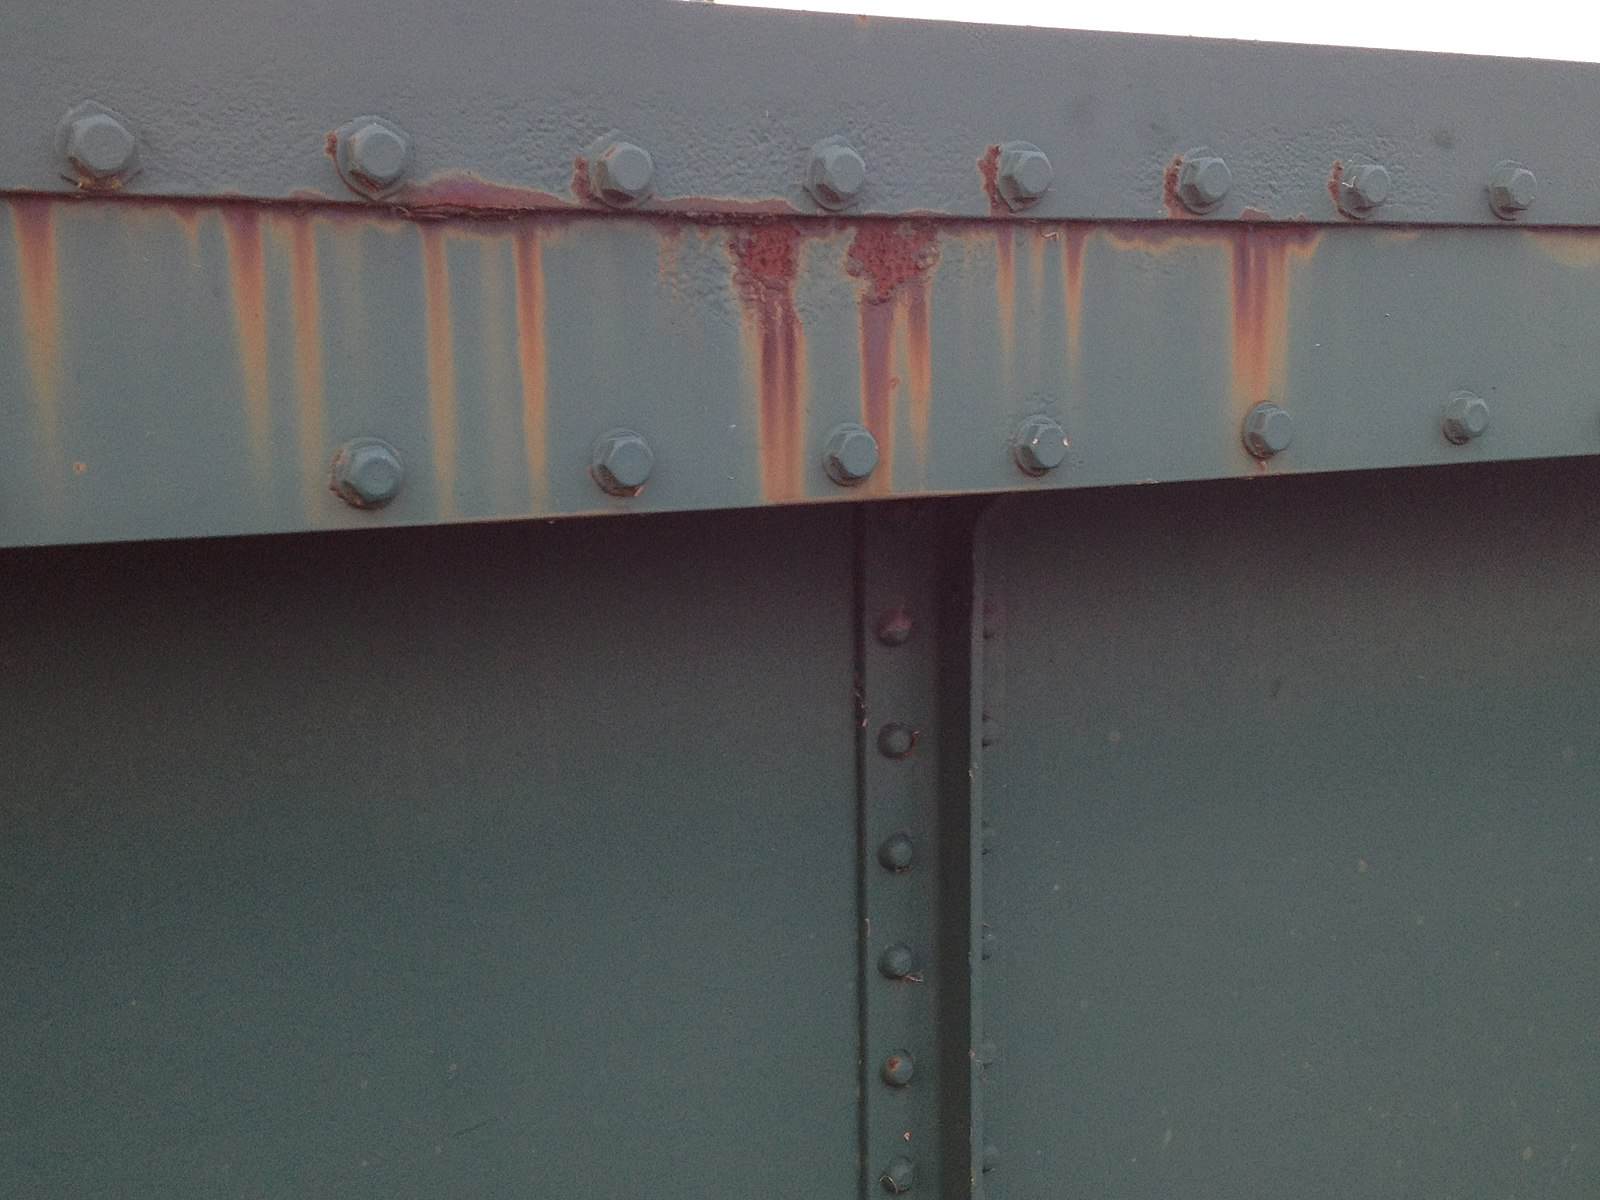
\includegraphics[width=0.45\columnwidth]{figures/applications/corrosion.jpg} \\[5pt]
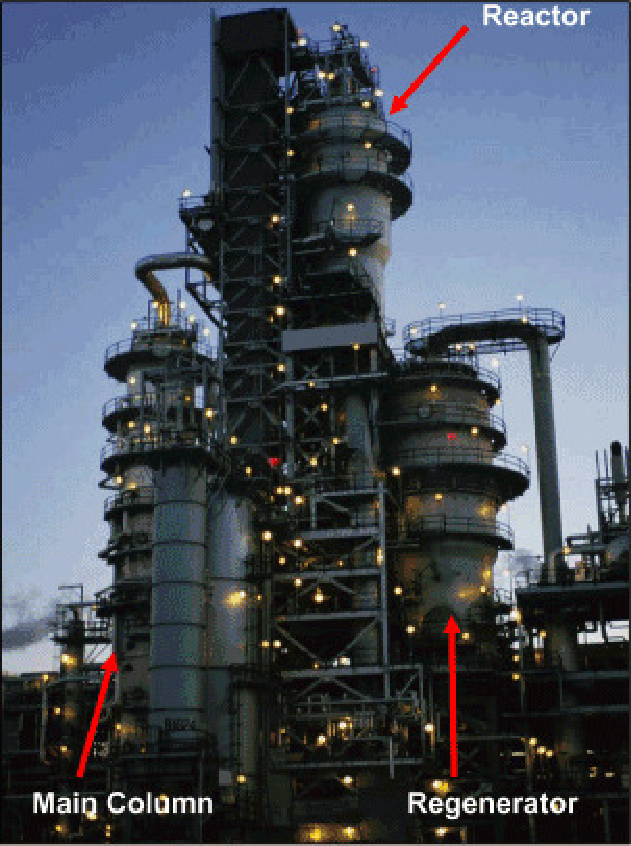
\includegraphics[width=0.45\columnwidth]{figures/applications/fluid-catalytic-cracker}
%\caption*{Hemoglobin structure.}
\end{figure}

\ecol

\end{frame}
%
% --------------------------------------------------------------------------------------------------------------------%
% Chemical equilibrium, Practical observations
% --------------------------------------------------------------------------------------------------------------------%
%
\subsection{Chemical equilibrium, Practical observations}
%
\begin{frame}{Chemical equilibrium, Practical observations}
	\vskip 10pt
\begin{itemize}
\item Chemical reactions \textbf{alter the amounts of species over time}, where species can be distributed among one or more phases (minerals, gaseous, mineral).
\pause
\item Each of these reactions have \textbf{forward and backward rates}. 
\pause
\item Consider the reaction
\[
\mathsf{A+B\rightleftharpoons C+2D,}
\]
\pause
\item Rate of the reaction is measured in mol/s.
\pause
\item Assume at some time $t$ this reaction has a \textbf{forward rate}
of \alert{\textbf{2 mol/s}} and a \textbf{backward rate}
of \alert{\textbf{1 mol/s}}.
\pause
\item \alert{\textbf{Net rate of the reaction}} = \textbf{forward rate} - \textbf{backward rate}. 
\end{itemize}
\end{frame}

\begin{frame}{Production and consumption rates}
	\vskip 10pt
Consider the reaction
	\[
	\mathsf{A+B\rightleftharpoons C+2D.}
	\]
%
\alert{\textbf{Question:}}  What is \textbf{rate of production\slash consumption}
of A, B, C and D (in mol/s)? \\
\begin{center}{ \href{http://etc.ch/M2Rp}{\textcolor{indigo(dye)}{\tt http://etc.ch/M2Rp}}} \quad
or \quad

\includegraphics[height=0.25\columnwidth]{figures/intro/poll.png}
\end{center}
\hiddenpause
\textbf{Answer:} \\
\qquad $\bullet$ production rates are 1 mol/s for C, 2 mol/s for D; \\
\qquad $\bullet$ consumption rates are -1 mol/s for A, -1 mol/s for B. 
\end{frame}
% --------------------------------------------------------------------------------------------------------------------%
% Chemical equilibrium of species
% --------------------------------------------------------------------------------------------------------------------%
%
\begin{frame}{Chemical equilibrium of species}
%
\alert{\textbf{Questions:}} What happens when this \textbf{net rate} is \alert{\textbf{zero}}? \\\textbf{Answer:} The amounts of each species in the system \textbf{no longer experience
any change}, and they are in \alert{\textbf{chemical equilibrium}}. \\[5pt]
%
\pause
\alert{\textbf{Example:}}
mixing 1 kg of H$_{2}$O with NaCl (halite):\\[-20pt] 
%
\begin{align*}
\mathsf{NaCl(halite, s)} & \rightleftharpoons\mathsf{Na^{+}+Cl^{-}}\\[-1pt]
\mathsf{Na^{+}+Cl^{-}} & \rightleftharpoons\mathsf{NaCl(aq)}\\[-1pt]
\mathsf{H_{2}O} & \rightleftharpoons\mathsf{H^{+}+OH^{-}}
\end{align*}
%
\vskip -5pt
\pause
\begin{itemize}
%
\item If we take \alert{\textbf{1 mg of NaCl}}, eventually, all salt fully dissolves, so the net rate of production of Na$^{+}$ and C$^-$ becomes zero.
%%\item we have reached the \textbf{chemical equilibrium} of the system. 
%\end{itemize}
%
\pause
\item If we take \alert{\textbf{100 mg of NaCl }}: eventually, water solution will be saturated with the salt, so Na$^{+}$ and C$^-$  is precipitating NaCl with the similar rate as it is dissolving.
%%\item we have reached the \textbf{chemical equilibrium} of the system. 
%\end{itemize}
\end{itemize}
\pause
\alert{\textbf{Note}}: See a Jupyter notebook \href{https://github.com/mtsveta/reaktoro-v2-workshop/blob/main/tutorials/solubility/solubility-tablesalt-water.ipynb}{\textcolor{indigo(dye)}{\it On mixing table salt with water}}.

\end{frame}
%
% --------------------------------------------------------------------------------------------------------------------%
% Example of aqueous-gaseous reaction in equilibrium
% --------------------------------------------------------------------------------------------------------------------%
%
\begin{frame}{Example of aqueous-gaseous reactions in equilibrium}
	%
	\begin{itemize}
		\item Consider the following \alert{\bf CO$_{2}$ dissolution/exsolution reaction}:
	\[
	\mathsf{H_2O(aq) + CO_{2}(g) \rightleftharpoons HCO^-_3(aq) + H^+(aq)}
	\]
\vskip -10pt
\pause
\item This reaction is in equilibrium when CO$_{2}$(g) is \textbf{dissolving
}(\emph{from gas to solution}) and \textbf{exsolving} (\emph{from
solution to gas}) at the same rate. 
	\pause
\item Alternatively, we can have the following \alert{\bf aqueous-gaseous reaction}:
%
\[
\mathsf{CO_{2}(g) \rightleftharpoons CO_2(aq)}
\]
\vskip -10pt
%
	\pause
\item \alert{\textbf{Good to know:}} The \textbf{solubility of
CO$_{2}$} (i.e., the maximum amount of CO$_{2}$ that the solution
can dissolve at given temperature, pressure, and fluid composition
conditions) can be calculated considering this reaction (and all others)
in equilibrium.
\end{itemize}
%
	\pause
\alert{\textbf{Note}}: See a tutorial \href{https://reaktoro.org/applications/miscellaneous/opening-bottle-with-sparkling-water.html}{\textcolor{indigo(dye)}{\it On mixing table salt with water}} with Jupyter notebook \href{https://github.com/mtsveta/reaktoro-v2-workshop/blob/main/tutorials/applications/opening-bottel-with-soda.ipynb}{\textcolor{indigo(dye)}{\it here}}.
%
\end{frame}
%
% --------------------------------------------------------------------------------------------------------------------%
% Example of aqueous-mineral reaction in equilibrium
% --------------------------------------------------------------------------------------------------------------------%
%
\begin{frame}[<+->]{Example of aqueous-mineral reaction in equilibrium}
\begin{itemize}
\item Consider the following calcite dissolution/precipitation \textbf{heterogeneous} reaction:
\[
\mathrm{\mathsf{CaCO_{3}(s,calcite) \rightleftharpoons Ca^{2+}(aq)+CO_{3}^{2-}(aq)}}
\]
\item This reaction is in equilibrium when calcite is \textbf{dissolving
}(\emph{from solid to solution}) and \textbf{precipitating} (\emph{from
solution to solid}) at the same rate. 
\item \textbf{\alert{\textbf{Good to know:}}} The \textbf{solubility of
calcite} (i.e., the maximum amount of calcite that the solution can
dissolve at given temperature, pressure, and fluid composition conditions)
can be calculated considering this reaction (and others) in equilibrium.
\end{itemize}
\end{frame}

% --------------------------------------------------------------------------------------------------------------------%
% Defining the chemical system in each geochemical modeling problem
% --------------------------------------------------------------------------------------------------------------------%
%
\subsection{Defining the chemical system in the geochemical modeling problem}
%
\begin{frame}{Defining the chemical system for the modeling problem}
\begin{itemize}
\item A chemical system is a collection of phases (one or more). Examples:
\begin{itemize}
\item a chemical system with only an aqueous phase;
\item a chemical system with aqueous and gaseous phase (CO$_2$(g));
\item a chemical system with aqueous, gaseous, and mineral phases.
\end{itemize}
\pause
\item Each phase has one or more chemical species:
\begin{itemize}
\item aqueous: H$_{2}$O(aq), H$^{+}$(aq), OH$^{-}$(aq), HCO$_{3}^{-}$(aq),
CO$_{3}^{2-}$(aq), CO$_{2}$(aq), Ca$^{2+}$(aq)
\item gaseous: H$_{2}$O(g), CO$_{2}$(g), O$_{2}$(g), H$_{2}$S(g)
\item calcite: CaCO$_{3}$(s)
\item solids: combination of several minerals, e.g., Granite: 30\% of Calcite, 33\% of Albite, 32\% of K-Feldspar, 5\% of Muscovite. 
\item oil
\item biomass (to simulate life of bacterias)
\end{itemize}
\pause
\item In geochemical modeling, suitable phases and their species need to
be considered. They must be added either: 
\begin{itemize}
\item manually (naming each species separately, e.g., [`H2O(l)', `H+', `OH-', `Na+', ...]) or 
\item automatically from databases (load all the species containing elements [`H', `O', `C']).
\end{itemize}
\end{itemize}
\end{frame}
%
% --------------------------------------------------------------------------------------------------------------------%
% Demonstration of chemical system definition
% --------------------------------------------------------------------------------------------------------------------%
%
\begin{frame}[fragile, allowframebreaks]{Demonstration of chemical system definition}
	
\begin{lstlisting}[language=Python, caption=Chemical system definition]
from reaktoro import *

# Define the SUPCRT database
db = SupcrtDatabase("supcrtbl")

# Define an aqueous solution
solution = AqueousPhase(speciate("H O Na Cl Ca C")) 

# Define gaseous phase
gas = GaseousPhase("CO2(g)")

# Define mineral phase
minerals = MineralPhases("Halite Calcite Dolomite Quartz")

# Create the chemical system
system = ChemicalSystem(db, solution, gas, minerals)

# Inspect species phases and species
for phase in system.phases():
    print(phase.name())
    for species in phase.species():
        print(":: " + species.name())
\end{lstlisting}
See also:
\begin{itemize}
    \item Reaktoro v2.0 Jupyter notebook tutorials on the Reaktoro website \href{https://reaktoro.org/tutorials/basics/index.html}{\textcolor{indigo(dye)}{\it Basics}} or
    \item similar Jupyter notebook  \href{https://github.com/mtsveta/reaktoro-v2-workshop/tree/main/tutorials/basics}{\textcolor{indigo(dye)}{\it Basics}} with interactive version available via \href{https://mybinder.org/v2/gh/mtsveta/reaktoro-v2-workshop/main?labpath=overview.ipynb}{\textcolor{indigo(dye)}{\it MyBinder Reaktoro v2.0}} or 
    \item \href{https://polybox.ethz.ch/index.php/s/qStBnxUnry648U5}{\textcolor{indigo(dye)}{\it explanation videos}} for Reaktoro v1.
\end{itemize}
%
\end{frame}


% --------------------------------------------------------------------------------------------------------------------%
% Example of the chemical system when substances H2O and CO2 are involved
% --------------------------------------------------------------------------------------------------------------------%
%
\begin{frame}{Example of the chemical system when H$_{2}$O and CO$_{2}$ are involved}

\lcol
\begin{itemize}
\item Assume water (H$_{2}$O) and carbon dioxide (CO$_{2}$), are mixed
at given T and P. 
\pause
\item To model the equilibrium state resulting from this process, the first
step is to think about:
\begin{itemize}
\item the possible phases of matter that could exist; and
\item the species in each phase. 
\end{itemize}
%
\pause
\item \alert{\textbf{Questions we are interested in}}: 
\begin{itemize}
\item Is CO$_{2}$ fully dissolved, or is it still present as a gas (water is already fully saturated with it)?
\item What are the amounts of each species in the chemical state after equilibration?
\end{itemize}
\end{itemize}
\rcol
\begin{itemize}
\item A simple (but reasonable) chemical system for this problem is:
\end{itemize}
\begin{center}
\begin{tabular}{cc}
\toprule 
\textbf{Aqueous Phase} & \textbf{Gaseous Phase}\tabularnewline
\midrule
H$_{2}$O(aq) & H$_{2}$O(g)\tabularnewline
H$^{+}$(aq) & CO$_{2}$(g)\tabularnewline
OH$^{-}$(aq) & \tabularnewline
HCO$_{3}^{-}$(aq) & \tabularnewline
CO$_{3}^{2-}$(aq) & \tabularnewline
CO$_{2}$(aq) & \tabularnewline
\bottomrule
\end{tabular}
\par\end{center}

\ecol
\end{frame}
%
% --------------------------------------------------------------------------------------------------------------------%
% Example of the chemical system when H2O and CaCO3 are involved
% --------------------------------------------------------------------------------------------------------------------%
%
\begin{frame}{Example of the chemical system when H$_{2}$O and CaCO$_{\boldsymbol{3}}$
are involved}
\begin{itemize}
\item Assume water (H$_{2}$O) and calcite (CaCO$_{3}$) are mixed at some
given temperature $T$ and pressure $P$.
\item A simple (but reasonable) chemical system for this problem is:
\end{itemize}
\begin{center}
\begin{tabular}{cc}
\toprule 
\multicolumn{1}{c}{\textbf{Aqueous Phase}} & \textbf{Calcite Phase}\tabularnewline
\midrule
H$_{2}$O(aq) & CaCO$_{3}$(s, calcite)\tabularnewline
H$^{+}$(aq) & \tabularnewline
OH$^{-}$(aq) & \tabularnewline
HCO$_{3}^{-}$(aq) & \tabularnewline
CO$_{3}^{2-}$(aq) & \tabularnewline
CO$_{2}$(aq) & \tabularnewline
Ca$^{2+}$(aq)  & \tabularnewline
\bottomrule
\end{tabular}
\par\end{center}

\end{frame}
%
% --------------------------------------------------------------------------------------------------------------------%
% Example of the chemical system when H2O, NaCl and CO2 are involved
% --------------------------------------------------------------------------------------------------------------------%
%
\begin{frame}{Example of the chemical system when H$_{2}$O, NaCl, and CO$_{2}$
are involved}
\begin{itemize}
\item Assume water (H$_{2}$O), carbon dioxide (CO$_{2}$), and sodium chloride
(NaCl), are mixed at some given temperature T and pressure P.
\pause 
\item A simple (but reasonable) chemical system for this problem is:
\end{itemize}
\begin{center}
\begin{tabular}{cccc}
\toprule 
\multicolumn{2}{c}{\textbf{Aqueous Phase}} & \multicolumn{1}{c}{\textbf{Gaseous Phase}} & \textbf{Halite Phase}\tabularnewline
\midrule
H$_{2}$O(aq) & CO$_{2}$(aq) & CO$_{2}$(g) & NaCl(s, halite)\tabularnewline
H$^{+}$(aq) & HCO$_{3}^{-}$(aq) & H$_{2}$O(g) & \tabularnewline
OH$^{-}$(aq) & CO$_{3}^{2-}$(aq) &  & \tabularnewline
Na$^{+}$(aq) &  NaCl(aq) &  & \tabularnewline
Cl$^{-}$(aq) &  &  & \tabularnewline
\bottomrule
\end{tabular}
\par\end{center}
\pause
\begin{itemize}
\item \alert{\textbf{We wan to know}}: 
\begin{itemize}
\item How does the salinity of the brine impact the solubility of the water? 
\item What happens if we put too much of the table salt? 
\item The phase of halite is significant to provide realistic estimation!
 because it has a point of solubility in water. 
\end{itemize}
\end{itemize}


\end{frame}
%
% --------------------------------------------------------------------------------------------------------------------%
% How many phases and species to consider for our chemical system?
% --------------------------------------------------------------------------------------------------------------------%
%
\begin{frame}{How many phases and species to consider for our chemical system?}

\lcol

\small
\begin{itemize}[<+->]
\item In general, the \textbf{number of phases and species} should be \textbf{as
large as possible} when \emph{defining a chemical system}.
\item However, the calculations get more expensive with increasing number
of species and phases.
\item \textbf{\alert{\textbf{Important:}}} Not all phases considered in
the calculation will actually exist in positive amounts. Their existence
depends on the input conditions.
\item The ternary phase diagram on the right shows conditions in which not
all phases are \textbf{stable at equilibrium}.
\end{itemize}
\rcol
\begin{figure}
\centering
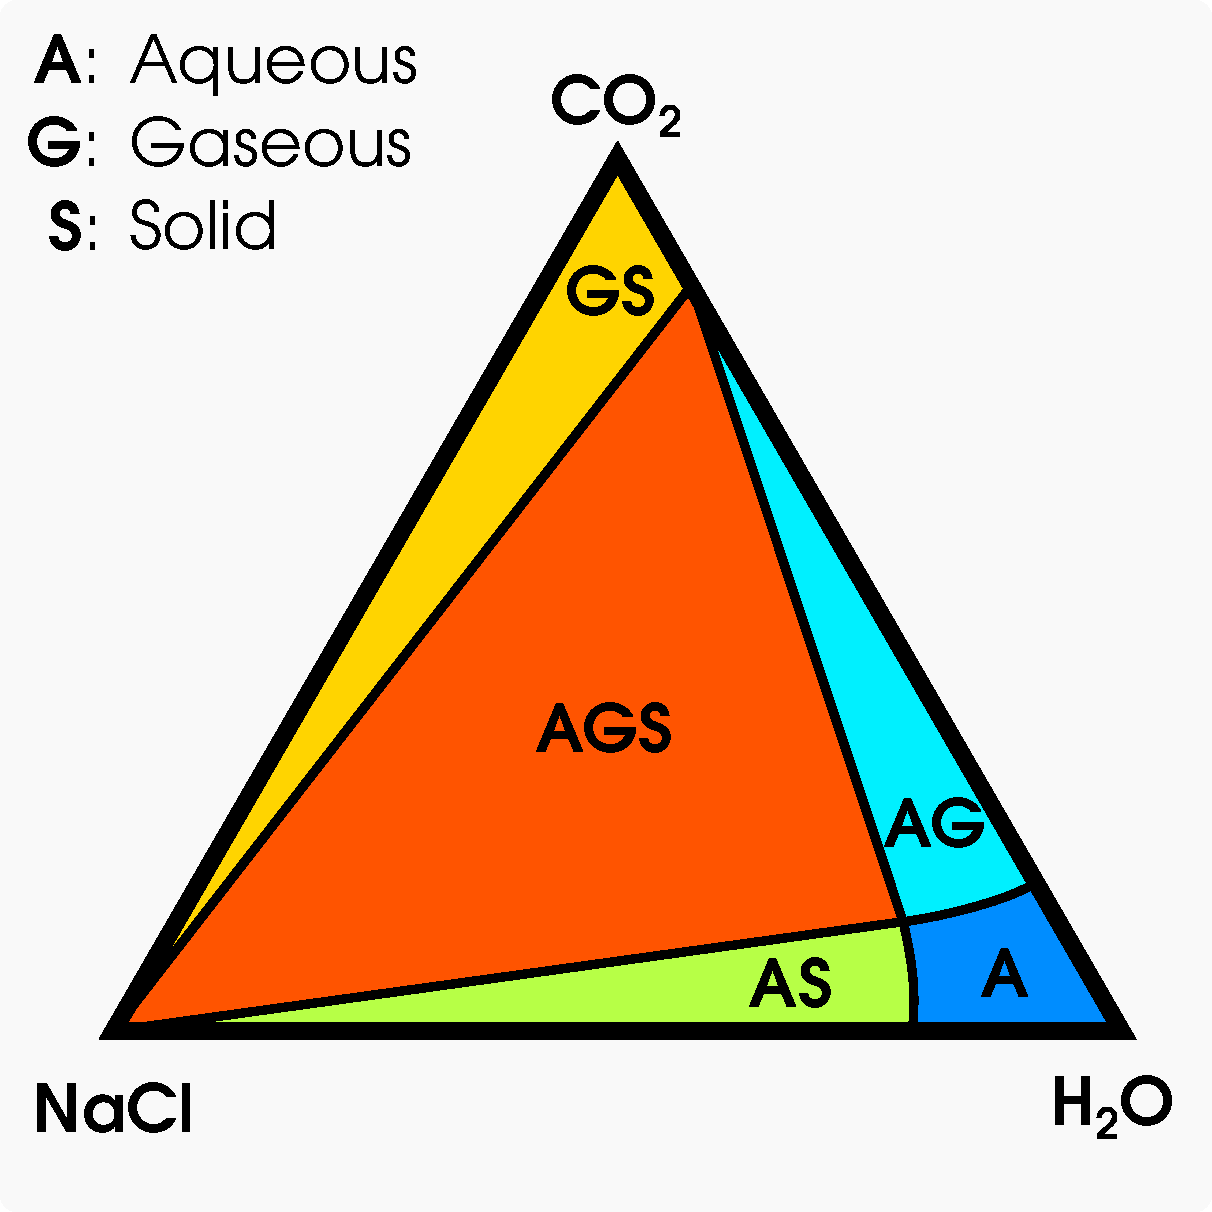
\includegraphics[width=0.9\columnwidth]{figures/applications/ternary-phase-diagram-h2o-co2-nacl}
\caption*{Ternary phase diagram.}
\end{figure}

\ecol
\end{frame}
%
% --------------------------------------------------------------------------------------------------------------------%
% Final considerations about defining the chemical system
% --------------------------------------------------------------------------------------------------------------------%
%
\begin{frame}{Final considerations about defining the chemical system}
	\vskip 10pt
\begin{itemize}
\item In most computer codes for modeling geochemical reactions, no manual
selection of phases and species are needed. 
\pause
\item These can be determined \textbf{automatically} by searching in \textbf{thermodynamic
databases} all possible species and phases that could exist for a
given model input. 
\pause
\item Depending on the available database, you can model different things: 
\begin{itemize}
\item supcrt98.xml
\item supcrt98-organics.xml (includes organic species)
\item thermofun.json (T = 200 °C, critical temperatures and pressures of gases used in Peng-Robinson's EOS) 
\item ColdChem.dat (a low-temperature aqueous thermodynamic model)
\end{itemize}

\end{itemize}
\end{frame}

%
\section{Chemical equilibrium from a thermodynamic and mathematical perspective}

% --------------------------------------------------------------------------------------------------------------------%
% Chemical equilibrium from a thermodynamic perspective
% --------------------------------------------------------------------------------------------------------------------%
\subsection{Gibbs energy minimization and its constraints}
%
\begin{frame}{Chemical equilibrium from a thermodynamic perspective}
\begin{itemize}
\item A system under prescribed temperature $T$ and pressure $P$ is \textbf{in
chemical equilibrium} if its \textbf{Gibbs energy} $G$ is at a minimum. 
\begin{itemize}
\item This results from the \emph{second law of thermodynamic} that says
that a system tends to a state of maximum entropy $S$. 
\item The minimum Gibbs energy condition arises because $G := H - T\,S$, where
$H$ is enthalpy. 
\item \textbf{Note}: \\
\quad (i) \; \alert{\textbf{Entropy}} $S$ is the measure of a system's thermal energy per unit temperature that is unavailable for doing useful work. \\ 
\quad (ii)\; \alert{\textbf{Enthalpy}} $H$ is a property of a thermodynamic system, defined as the sum of the system's internal energy and the product of its pressure and volume, i.e, $H = E + P\, V$, where $E$ is the internal energy.
\end{itemize}
\pause
\item Analogy to the \textbf{mechanical equilibrium}: a \emph{ball rolling down a hill}. 
We want to find the \textbf{final position} of the ball that results in a minimum for its 
\textbf{potential energy}.
\pause
\item In thermodynamics, we want to find the \textbf{composition (amounts of each species)}, in every phase, that \textbf{minimizes the Gibbs energy} of the chemical system.
\end{itemize}
\end{frame}
%
% --------------------------------------------------------------------------------------------------------------------%
% Constraints in a chemical equilibrium state
% --------------------------------------------------------------------------------------------------------------------%
%
\begin{frame}{Constraints in a chemical equilibrium state}
\begin{itemize}
\item In \alert{\textbf{mechanical equilibrium}}, a ball rolling down a hill is \textbf{constrained by its surface topology}. 
\pause
\item In \textbf{thermodynamics}, the species in a chemical system seeking a state of chemical
equilibrium is also \textbf{constrained by some conditions}: 
\begin{itemize}
\item \textbf{its non-negativity} (species amounts cannot be negative),
\item \alert{\textbf{mass conservation}}.
\end{itemize}
\end{itemize}
\end{frame}
%
%
% --------------------------------------------------------------------------------------------------------------------%
% Mass conservation constraints in chemical equilibrium
% --------------------------------------------------------------------------------------------------------------------%
%
\begin{frame}{Mass conservation constraints in chemical equilibrium \, i}
%
\vskip 10pt
To illustrate \alert{\textbf{mass conservation constraints}} the following problem: 
\begin{itemize}
\item we mix 100 moles of H$_{2}$O and 2 moles of CO$_{2}$
and \textbf{calculate the equilibrium state of the system}, 
\item these two substances will react and form several species (H$^{+}$,
HCO$_{3}^{-}$ etc).
\end{itemize}
\hiddenpause
\alert{\textbf{Quiz}}: at chemical equilibrium, what can we tell about 
the amounts of H, O, C?

\begin{center}
\href{http://etc.ch/bv5y}{\textcolor{indigo(dye)}{\tt http://etc.ch/bv5y}} 
\quad
or 
\quad

\includegraphics[height=0.21\columnwidth]{figures/chemical-equilibrium/poll.png}
\end{center}

\hiddenpause
\textbf{Answer}: 200 moles of H, 104 moles of O, and 2 moles of C,  Z = 0 (the final charge must be equal to the initial charge). 
\end{frame}
%
\begin{frame}{Mass conservation constraints in chemical equilibrium\, ii}
	%
\begin{itemize}
		\item Calculating chemical equilibrium requires finding a composition for
		the system (i.e., amount of species, usually defined by vector 
		$n = [n_{\sf H^{+}}, n_{\sf HCO_{3}^{-}}, \ldots]$) that 
		\textbf{minimizes its Gibbs energy} and simultaneously satisfies 
		\alert{\textbf{mass conservation}} of
		\begin{itemize}
			\item \textbf{chemical elements} and
			\item \textbf{electric charge}.
		\end{itemize}
		\pause
		\item \alert{\textbf{Note}}: we use the term \alert{\textbf{elements}} represented by vector $b$ 
		to denote both \emph{chemical elements} and \emph{electric charge}, i.e., 
		$b = [b_{\sf H}, b_{\sf O}, b_{\sf C}, b_{\sf Z}]$.
	\end{itemize}
\end{frame}
%
% --------------------------------------------------------------------------------------------------------------------%
% Chemical equilibrium problem for the H2O–CO2 system
% --------------------------------------------------------------------------------------------------------------------%
%
\begin{frame}{Chemical equilibrium problem for the H$_{\boldsymbol{2}}$O–CO$_{\boldsymbol{2}}$
system}

\lcol

Given \emph{temperature} $T$, \emph{pressure} $P$ and the \emph{amounts
of elements} H, O, C, determine \\
the \textbf{amounts of the species at equilibrium}:
\begin{center}
\begin{tabular}{cc}
\toprule 
\multicolumn{1}{c}{\textbf{Aqueous Phase}} & \multicolumn{1}{c}{\textbf{Gaseous Phase}}\tabularnewline
\midrule
H$_{2}$O(aq) & CO$_{2}$(g)\tabularnewline
H$^{+}$(aq) & H$_{2}$O(g)\tabularnewline
OH$^{-}$(aq) & \tabularnewline
CO$_{3}^{2-}$(aq) & \tabularnewline
HCO$_{3}^{-}$(aq) & \tabularnewline
CO$_{2}$(aq) & \tabularnewline
\bottomrule
\end{tabular} 
\par\end{center}

\rcol
\pause
\vskip 5pt
\alert{\textbf{Questions:}}
\begin{itemize}
\item What are the amounts of each chemical species at equilibrium? 
\item Which phases exist at equilibrium? 
\item How much carbon dioxide CO$_{2}$(g) has dissolved as carbon-bearing
aqueous species, turned into CO$_{2}$(aq)? 
\item How much solvent water H$_{2}$O(aq) evaporated to the gas phase
as vapor H$_{2}$O(g)? 
\item What is the concentration of H$^{+}$(aq), which is related to pH
(acidity)?
\end{itemize}
\ecol
\end{frame}
%
% --------------------------------------------------------------------------------------------------------------------%
% Mass conservation constraints for the H2O–CO2 system at equilibrium
% --------------------------------------------------------------------------------------------------------------------%
%
\begin{frame}[<+->]{Mass conservation constraints for the H$_{\boldsymbol{2}}$O–CO$_{\boldsymbol{2}}$
system at equilibrium}
 
\begin{itemize}
\item At equilibrium, the amounts of the species
\[
n=(n_{\mathsf{H_{2}O\text{(aq)}}},\;n_{\mathsf{H^{+}\text{(aq)}}},\;n_{\mathsf{OH^{-}\text{(aq)}}},\;n_{\mathsf{CO_{3}^{2-}\text{(aq)}}},\;n_{\mathsf{HCO_{3}^{-}}\text{(aq)}},\;n_{\mathsf{CO_{2}\text{(aq)}}},\;n_{\mathsf{CO_{2}\text{(g)}}},\;n_{\mathsf{H_{2}O\text{(g)}}})
\]
must satisfy the \textbf{mass conservation equations} for each element:{\small{}
\begin{alignat}{1}
2n_{\mathsf{H_{2}O\text{(aq)}}}+n_{\mathsf{H^{+}\text{(aq)}}}+n_{\mathsf{OH^{-}\text{(aq)}}}+n_{\mathsf{HCO_{3}^{-}\text{(aq)}}}+2n_{\mathsf{H_{2}O\text{(g)}}} & =b_{\mathsf{H}}\\
n_{\mathsf{H_{2}O\text{(aq)}}}+n_{\mathsf{OH^{-}\text{(aq)}}}+3n_{\mathsf{CO_{3}^{2-}\text{(aq)}}}+3n_{\mathsf{HCO_{3}^{-}}\text{(aq)}}+2n_{\mathsf{CO_{2}\text{(aq)}}}+2n_{\mathsf{CO_{2}\text{(g)}}}+n_{\mathsf{H_{2}O\text{(g)}}} & =b_{\mathsf{O}}\\
n_{\mathsf{CO_{3}^{2-}\text{(aq)}}}+n_{\mathsf{HCO_{3}^{-}\text{(aq)}}}+n_{\mathsf{CO_{2}\text{(aq)}}}+n_{\mathsf{CO_{2}\text{(g)}}} & =b_{\mathsf{C}}\\
n_{\mathsf{H^{+}\text{(aq)}}}-n_{\mathsf{OH^{-}\text{(aq)}}}-2n_{\mathsf{CO_{3}^{2-}\text{(aq)}}}-n_{\mathsf{HCO_{3}^{-}\text{(aq)}}} & =b_{\mathsf{Z}}
\end{alignat}
}{\small\par}
\item For this specific system, we can show that 
the {\bf equation for electrical charge Z is linearly dependent} on
the other equations.
%\item \alert{\textbf{Hint}}: Show that the last row 
%(4) = (1) - 2 (2) + 4 (3).

\end{itemize}
\end{frame} 
%
% --------------------------------------------------------------------------------------------------------------------%
% Mass conservation constraints written in matrix form
% --------------------------------------------------------------------------------------------------------------------%
%
\begin{frame}{Mass conservation constraints written in matrix form}

The {\bf mass balance equations} can be written in matrix form: \\[10pt]

\begin{cbox}{Mass conservation equation in matrix form}{\Large{}
\[
An=b
\]
}\end{cbox}where:
\begin{itemize}
\item $A$ is the \textbf{formula matrix} of the system
\item $n=(n_{1},\ldots,n_{\text{N}})$ is the \textbf{vector of species
amounts}
\item $b=(b_{1},\ldots,b_{\text{E}})$ is the \textbf{vector of element
amounts}
\end{itemize}
\end{frame}
%
% --------------------------------------------------------------------------------------------------------------------%
% Constructing the formula matrix for the H2O–CO2 system
% --------------------------------------------------------------------------------------------------------------------%
%
\begin{frame}[<+->]{Constructing the formula matrix for the H$_{\boldsymbol{2}}$O–CO$_{\boldsymbol{2}}$ system\; i}

Consider the following ordering for species and elements in the system:
\begin{center}
\begin{tabular*}{1\textwidth}{@{\extracolsep{\fill}}ccccc}
\toprule 
\textbf{Index} & \textbf{Species} &  & \textbf{Index} & \textbf{Element}\tabularnewline
\midrule
0 & H$_{2}$O(aq) &  & 0 & H\tabularnewline
1 & H$^{+}$(aq) &  & 1 & O\tabularnewline
2 & OH$^{-}$(aq) &  & 2 & C\tabularnewline
3 & CO$_{3}^{2-}$(aq) &  & 3 & Z\tabularnewline
4 & HCO$_{3}^{-}$(aq) &  &  & \tabularnewline
5 & CO$_{2}$(aq) &  &  & \tabularnewline
6 & CO$_{2}$(g) &  &  & \tabularnewline
7 & H$_{2}$O(g) &  &  & \tabularnewline
\bottomrule
\end{tabular*}
\par\end{center}

\alert{\textbf{Exercise:}} Construct the formula matrix $A$ for this system, where \\
\alert{\textbf{the coefficient $A_{ji}$ characterises the contribution of species 
$i$ into the element $j$}}. 
\end{frame}
%
% --------------------------------------------------------------------------------------------------------------------%
% Constructing the formula matrix for the H2O–CO2 system
% --------------------------------------------------------------------------------------------------------------------%

\begin{frame}{Constructing the formula matrix for the H$_{\boldsymbol{2}}$O-CO$_{\boldsymbol{2}}$ system\; ii}

\textbf{Answer:} {\small
$$A=\kbordermatrix{
& \mathclap{\mathsf{H_2O(aq)}} & \mathclap{\mathsf{H^+(aq)}} & \mathclap{\mathsf{OH^-(aq)}} & \mathclap{\mathsf{CO_3^{2-}(aq)}} & \mathclap{\mathsf{HCO_3^-(aq)}} & \mathclap{\mathsf{CO_2(aq)}} & \mathclap{\mathsf{CO_2(g)}}  & \mathclap{\mathsf{H_2O(g)}}\\
\mathsf{H} & \w{2} & \w{1} & \w{1} & \w{0} & \w{1} & \w{0} & \w{0} & \w{2}\\
\mathsf{O} & 1 & 0 & 1 & 3 & 3 & 2 & 2 & 1\\
\mathsf{C} & 0 & 0 & 0 & 1 & 1 & 1 & 1 & 0\\
\mathsf{Z} & 0 & 1 & \minus{1} & \minus{2} & \minus{1} & 0 & 0 & 0
}
$$}

\hiddenpause

\lcol

\alert{\textbf{Quiz:}} Which of the following linearly dependency relation
is true for the rows of $A$:

\vskip 5pt
\visible<2->{
\centering
\href{http://etc.ch/bv5y}{\textcolor{indigo(dye)}{\tt  http://etc.ch/bv5y}} \quad or \quad 

\includegraphics[height=0.35\columnwidth]{figures/chemical-equilibrium/poll.png}}

\rcol

\vspace{-4ex}
\visible<2->{
{\small{}
\begin{alignat*}{2}
\text{(1)} & \quad & \text{row(Z)} & =\text{row(H)}-2\,\text{row(O)}\\
\text{(2)} &  & \text{row(Z)} & =\text{row(H)}-2\,\text{row(O)}+2\,\text{row(C)}\\
\text{(3)} &  & \text{row(Z)} & =\text{row(H)}-2\,\text{row(O)}+4\,\text{row(C)}\\
\text{(4)} &  & \text{row(Z)} & =\text{row(H)}-2\,\text{row(O)}+6\,\text{row(C)}
\end{alignat*}
}{\small\par}
}
\visible<3->{
\textbf{Answer:} (3)
}
\ecol
\end{frame}

% --------------------------------------------------------------------------------------------------------------------%
% Calculating the amounts of elements from species amounts
% --------------------------------------------------------------------------------------------------------------------%
%
\begin{frame}{Calculating the amounts of elements from species amounts}

\vskip 10pt
\lcol[0.7]

\alert{\textbf{Exercise:}} Given 
\[
n=\left[\begin{array}{l}
n_{\mathsf{H_{2}O\text{(}aq\text{)}}}\\
n_{\mathsf{H^{+}\text{(}aq\text{)}}}\\
n_{\mathsf{OH^{-}\text{(}aq\text{)}}}\\
n_{\mathsf{CO_{3}^{2-}\text{(}aq\text{)}}}\\
n_{\mathsf{HCO_{3}^{-}\text{(}aq\text{)}}}\\
n_{\mathsf{CO_{2}\text{(}aq\text{)}}}\\
n_{\mathsf{CO_{2}\text{(}g\text{)}}}\\
n_{\mathsf{H_{2}O\text{(}g\text{)}}}
\end{array}\right]=\begin{bmatrix}n_{0}\\
n_{1}\\
n_{2}\\
n_{3}\\
n_{4}\\
n_{5}\\
n_{6}\\
n_{7}
\end{bmatrix}=\begin{bmatrix}55.4551\\
1.23485\cdot10^{-4}\\
8.39739\cdot10^{-11}\\
4.93648\cdot10^{-11}\\
1.23484\cdot10^{-4}\\
0.032861\\
1.96702\\
0.0531732
\end{bmatrix},
\]

\rcol[0.3]
calculate
\[
b=\left[\begin{array}{l}
b_{\mathsf{H}}\\
b_{\mathsf{O}}\\
b_{\mathsf{C}}\\
b_{\mathsf{Z}}
\end{array}\right] = A \, n.
\]
\ecol
\vskip 10pt
%\visible<2->{If we have vector $n$ and matrix $A$ we can compute $b = A n$.} \\
\visible<2->{Instead of doing such calculation manually (tedious and error prone), let's use \textbf{Python}: 
\begin{itemize}
\item for Python shell, you can use an online tool \href{http://repl.it/languages/python}{\textcolor{indigo(dye)}{\tt repl.it/languages/python}}
\item Python source code can be downloaded from \href{https://polybox.ethz.ch/index.php/s/ku86DyuR6nvW2Zl}{\textcolor{indigo(dye)}{\it mass-balance-with-blanks.py}}.
\end{itemize}
}
\end{frame}
%
% --------------------------------------------------------------------------------------------------------------------%
% Calculating the amounts of elements using Python
% --------------------------------------------------------------------------------------------------------------------%
%
\begin{frame}[fragile, allowframebreaks]{Calculating the amounts of elements using Python -- Source}

\lstinputlisting[language=Python, caption=Calculating the amounts of elements using Python]{python-files/mass-balance-with-blanks.py}	

% Source code: \href{https://polybox.ethz.ch/index.php/s/ku86DyuR6nvW2Zl}{\textcolor{indigo(dye)}{\it link}}.
\end{frame}
%
% --------------------------------------------------------------------------------------------------------------------%
% Calculating the amounts of elements using Python – Output
% --------------------------------------------------------------------------------------------------------------------%
%
\begin{frame}[fragile]{Calculating the amounts of elements using Python -- Output}

The Python code has to have the following output:

\begin{lstlisting}[language=Python, caption=Calculating the amounts of elements using Python -- Output]
Element H has 111.0168 moles and 111.8938 grams
Element O has 59.5084 moles and 952.0988 grams
Element C has 2.0000 moles and 24.0215 grams
Element Z has 0.0000 moles and 0.0000 grams

Species H2O(aq) has 5.5455e+01 moles and 9.9903e+02 grams
Species H+ has 1.2349e-04 moles and 1.2446e-04 grams
Species OH- has 8.3974e-11 moles and 1.4282e-09 grams
Species CO3-- has 4.9365e-11 moles and 2.9623e-09 grams
Species HCO3- has 1.2348e-04 moles and 7.5346e-03 grams
Species CO2(aq) has 3.2861e-02 moles and 1.4462e+00 grams
Species CO2(g) has 1.9670e+00 moles and 8.6568e+01 grams
Species H2O(g) has 5.3173e-02 moles and 9.5793e-01 grams
\end{lstlisting}

\textbf{Answer}: To check the correctness of the gaps in the code, use the  \href{https://polybox.ethz.ch/index.php/s/sVotdOJMkp740Lw}{\textcolor{indigo(dye)}{\it source code}}.

\end{frame}
%
% --------------------------------------------------------------------------------------------------------------------%
% Chemical equilibrium formulated as Gibbs energy minimization problem
% --------------------------------------------------------------------------------------------------------------------%
%
\begin{frame}{Chemical equilibrium formulated as Gibbs energy minimization problem}
%
\begin{cbox}{Gibbs energy minimization (GEM) problem}

Given temperature $T$, pressure $P$, and amounts of elements ${b=(b_{1},\ldots,b_{\text{E}})}$,
find the amounts of species ${n=(n_{1},\ldots,n_{\text{N}})}$ that
solve the \textbf{constrained minimization problem}:
\[
\min_{n}G(n;T,P)\qquad\text{subject to}\qquad An=b\quad\text{and}\quad n\geq0.
\]

\end{cbox}where:

\begin{itemize}
\item $G$ is the Gibbs energy of the system, a function of $n=(n_{1},\ldots,n_{\text{N}})$
as well as temperature $T$ and pressure $P$;
\item $An=b$ are the mass conservation constraints for each element;
\item $n\geq0$ are the non-negative constraints for the amounts of each
species.
\end{itemize}
\end{frame}
%
\begin{frame}{Gibbs energy function}

\begin{itemize}
\item 
\textbf{The Gibbs energy function}, $G$, is defined as: 
\[
\boxed{
G=\sum_{i=1}^{\text{N}}n_{i}\mu_{i},
}
\]
where $\mu_{i}$ is the \alert{\bf chemical potential} of the $i$th
species. \\[30pt]
%\hiddenpause
%\item \textbf{Question:} What is the dimension (in SI units) of $G$ and
%$\mu_{i}$? 
%\hiddenpause
\item $G$ has units of J, and $\mu_{i}$ units of J/mol.
\end{itemize}
\end{frame}
%
% --------------------------------------------------------------------------------------------------------------------%
% Chemical potential and its interpretation
% --------------------------------------------------------------------------------------------------------------------%
%
\subsection{Chemical potential of chemical species}
%
\begin{frame}{Chemical potential and its interpretation}

\begin{itemize}
\item The \textbf{chemical potential of a substance $\mu_{i}$} is a measure of
its tendency to transform into other substances.
\pause
\item In the following reaction:
\[
\mathsf{A\rightleftharpoons B},
\]

\begin{itemize}
\item $\mu_{\sf A}>\mu_{\sf B}$: substance A will tend to transform to B 
\item $\mu_{\sf A}=\mu_{\sf B}$: substances A and B are in equilibrium, no
transformation is happening
\item $\mu_{\sf A}<\mu_{\sf B}$: substance B will tend to transform to A
\end{itemize}
\pause
\item The higher the value of $\mu_{\sf A}$, the higher the tendency for A
to transform to B.
\end{itemize}
\end{frame}
%
% --------------------------------------------------------------------------------------------------------------------%
% Chemical potential and its interpretation – Example
% --------------------------------------------------------------------------------------------------------------------%
%
\begin{frame}{Chemical potential and its interpretation, Example}
\begin{itemize}
\item Consider the following reaction:
\[
\mathsf{CO_{2}\text{(g)}\rightleftharpoons CO_{2}\text{(aq)}}
\]
\vskip -50pt

\includegraphics[height=0.17\columnwidth,right]{figures/chemical-equilibrium/poll.png}
\pause
\vskip -40pt
\item We have the following three cases: 
{
\footnotesize{}
\begin{align*}
\text{\textbf{Case I}} &  & \textbf{Case II} &  & \textbf{Case III}\\
\mu_{\mathsf{CO_{2}\text{(g)}}} & = -390.347\,{\mathsf{kJ/mol}} & 
\mu_{\mathsf{CO_{2}\text{(g)}}} & = -390.347\,{\mathsf{kJ/mol}} & 
\mu_{\mathsf{CO_{2}\text{(g)}}} & = -389.185\,{\mathsf{kJ/mol}}\\
\mu_{\mathsf{CO_{2}\text{(aq)}}} & = -390.347\,{\mathsf{kJ/mol}} & \mu_{\mathsf{CO_{2}\text{(aq)}}} & = -517.800\,{{\mathsf{kJ/mol}}} & \mu_{\mathsf{CO_{2}\text{(aq)}}} & =-383.861\,{\mathsf{kJ/mol}}
\end{align*}
}{\footnotesize\par}
\vskip 10pt 
%
\pause
\item \alert{\textbf{Quiz}}: what is the tendency for CO$_{2}$(g) in each of cases?
%
\hiddenpause

\item \alert{\textbf{Answer}}:
\begin{itemize}
\item \textbf{Case I}: Since $\mu_{\mathsf{CO_{2}\text{(g)}}}=\mu_{\mathsf{CO_{2}\text{(aq)}}}$,
the reaction is in \textbf{equilibrium}.
\item \textbf{Case II}: Since $\mu_{\mathsf{CO_{2}\text{(g)}}}>\mu_{\mathsf{CO_{2}\text{(aq)}}}$,
CO$_{2}$(g) tends to \textbf{dissolve}.
\item \textbf{Case III}: Since $\mu_{\mathsf{CO_{2}\text{(g)}}}<\mu_{\mathsf{CO_{2}\text{(aq)}}}$,
CO$_{2}$(g) tends to form, \textbf{exsolve}. \setbeamercovered{transparent}
\end{itemize}
\end{itemize}

\end{frame}
%
% --------------------------------------------------------------------------------------------------------------------%
% Chemical potentials and direction of reactions
% --------------------------------------------------------------------------------------------------------------------%
%
\begin{frame}{Chemical potentials and direction of reactions}

\begin{itemize}[<+->]
\item The chemical potentials of substances $\mu_{i}$ can be used to
indicate which direction a reaction should proceed: 
\[
\mathsf{A+B\rightleftharpoons C+2\,D}
\]
\item $\mu_{\sf A}+\mu_{\sf B}>\mu_{\sf C}+2\,\mu_{\sf D}$: substances A and B will
tend to transform to C and D
\item $\mu_{\sf A}+\mu_{\sf B}=\mu_{\sf C}+2\,\mu_{\sf D}$: substances A, B, C,
and D are in equilibrium 
\item $\mu_{\sf A}+\mu_{\sf B}<\mu_{\sf C}+2\,\mu_{\sf D}$: substances C and D will
tend to transform to A and B
\item \alert{\bf Note:} the coefficients in the reactions are used
when checking the direction of the reaction!
\[
\mathsf{\underline{1}\,A+\underline{1}\,B\rightleftharpoons\underline{1}\,C+\underline{2}\,D}
\]
\end{itemize}
\end{frame}
%
% --------------------------------------------------------------------------------------------------------------------%
% Chemical potentials and direction of reactions
% --------------------------------------------------------------------------------------------------------------------%
%
\begin{frame}{Chemical potentials and direction of reactions, Exercise \; i}

Consider the following reaction and the subsequent
three cases:{
\[
\mathsf{H_{2}O(aq)+CO_{2}(g)\rightleftharpoons HCO_{3}^{-}(aq)+H^{+}(aq)}
\]
}\vspace{-4ex}
{\small{}
\begin{align*}
\text{\textbf{Case I}} &  & \textbf{Case II} &  & \textbf{Case III}\\
\mu_{\mathsf{H_{2}O\text{(aq)}}} & = -239.614\,{\mathsf{kJ/mol}} & 
\mu_{\mathsf{H_{2}O\text{(aq)}}} & = -239.614\,{\mathsf{kJ/mol}} & 
\mu_{\mathsf{H_{2}O\text{(aq)}}} & = -239.614\,{\mathsf{kJ/mol}}\\
\mu_{\mathsf{CO_{2}\text{(g)}}} & = -390.347\,{\mathsf{kJ/mol}} & 
\mu_{\mathsf{CO_{2}\text{(g)}}} & = -390.347\,{\mathsf{kJ/mol}} & 
\mu_{\mathsf{CO_{2}\text{(g)}}} & = -389.185\,{\mathsf{kJ/mol}}\\
\mu_{\mathsf{HCO_{3}^{-}\text{(aq)}}} & = -610.019\,{\mathsf{kJ/mol}} & 
\mu_{\mathsf{HCO_{3}^{-}\text{(aq)}}} & = -717.639\,{\mathsf{kJ/mol}} & 
\mu_{\mathsf{HCO_{3}^{-}\text{(aq)}}} & = -606.776\,{\mathsf{kJ/mol}}\\
\mu_{\mathsf{H^{+}\text{(aq)}}} & = -19.942\,{\mathsf{kJ/mol}} & 
\mu_{\mathsf{H^{+}\text{(aq)}}} & = -41.454\,{\mathsf{kJ/mol}} & 
\mu_{\mathsf{H^{+}\text{(aq)}}} & = -16.699\,{\mathsf{kJ/mol}}
\end{align*}
}{\small\par}
\pause
\alert{\textbf{Quiz}}:
\begin{itemize}
\item What is the direction of the reaction in each case?
\item In each case, is CO$_{2}$(g) tending to dissolve or exsolve? 
\end{itemize}
\vskip -45pt

\includegraphics[height=0.16\columnwidth,right]{figures/chemical-equilibrium/poll.png}
\end{frame}
%
% --------------------------------------------------------------------------------------------------------------------%
% Chemical potentials and direction of reactions
% --------------------------------------------------------------------------------------------------------------------%
%
\begin{frame}{Chemical potentials and direction of reactions, Exercise \; ii}

\textbf{Case I: }

\lcol
\begin{align*}
\mu_{\mathsf{H_{2}O\text{(aq)}}} & =\unit[-239.614]{\mathsf{kJ/mol}}\\
\mu_{\mathsf{CO_{2}\text{(g)}}} & =\unit[-390.347]{\mathsf{kJ/mol}}\\
\mu_{\mathsf{HCO_{3}^{-}\text{(aq)}}} & =\unit[-610.019]{\mathsf{kJ/mol}}\\
\mu_{\mathsf{H^{+}\text{(aq)}}} & =\unit[-19.942]{\mathsf{kJ/mol}}
\end{align*}
\rcol

\begin{align*}
\mu_{\mathsf{H_{2}O\text{(aq)}}}+\mu_{\mathsf{CO_{2}\text{(g)}}} & =-629.961\\
\mu_{\mathsf{HCO_{3}^{-}\text{(aq)}}}+\mu_{\mathsf{H^{+}\text{(aq)}}} & =-629.961
\end{align*}
\[
\boxed{\mu_{\mathsf{H_{2}O\text{(aq)}}}+\mu_{\mathsf{CO_{2}\text{(g)}}}=\mu_{\mathsf{HCO_{3}^{-}\text{(aq)}}}+\mu_{\mathsf{H^{+}\text{(aq)}}}}
\]

The reaction is in \textbf{equilibrium}.

\ecol
\end{frame}
%
% --------------------------------------------------------------------------------------------------------------------%
% Chemical potentials and direction of reactions, IV
% --------------------------------------------------------------------------------------------------------------------%
%
\begin{frame}{Chemical potentials and direction of reactions, Exercise \; iii}

\textbf{Case II: }

\lcol
\begin{align*}
\mu_{\mathsf{H_{2}O\text{(aq)}}} & =\unit[-239.614]{\mathsf{kJ/mol}}\\
\mu_{\mathsf{CO_{2}\text{(g)}}} & =\unit[-390.347]{\mathsf{kJ/mol}}\\
\mu_{\mathsf{HCO_{3}^{-}\text{(aq)}}} & =\unit[-717.639]{\mathsf{kJ/mol}}\\
\mu_{\mathsf{H^{+}\text{(aq)}}} & =\unit[-41.454]{\mathsf{kJ/mol}}
\end{align*}
\rcol

\begin{align*}
\mu_{\mathsf{H_{2}O\text{(aq)}}}+\mu_{\mathsf{CO_{2}\text{(g)}}} & =-629.961\\
\mu_{\mathsf{HCO_{3}^{-}\text{(aq)}}}+\mu_{\mathsf{H^{+}\text{(aq)}}} & =-759.093
\end{align*}
\[
\boxed{\mu_{\mathsf{H_{2}O\text{(aq)}}}+\mu_{\mathsf{CO_{2}\text{(g)}}}>\mu_{\mathsf{HCO_{3}^{-}\text{(aq)}}}+\mu_{\mathsf{H^{+}\text{(aq)}}}}
\]

The reaction is proceeding to the right, and CO$_{2}$ is tending
to \textbf{dissolve}.

\ecol
\end{frame}
%
% --------------------------------------------------------------------------------------------------------------------%
% Chemical potentials and direction of reactions, V
% --------------------------------------------------------------------------------------------------------------------%
%
\begin{frame}{Chemical potentials and direction of reactions , Exercise \; iv}

\textbf{Case III: }

\lcol
\begin{align*}
\mu_{\mathsf{H_{2}O\text{(aq)}}} & =\unit[-239.614]{\mathsf{kJ/mol}}\\
\mu_{\mathsf{CO_{2}\text{(g)}}} & =\unit[-390.347]{\mathsf{kJ/mol}}\\
\mu_{\mathsf{HCO_{3}^{-}\text{(aq)}}} & =\unit[-717.639]{\mathsf{kJ/mol}}\\
\mu_{\mathsf{H^{+}\text{(aq)}}} & =\unit[-41.454]{\mathsf{kJ/mol}}
\end{align*}
\rcol

\begin{align*}
\mu_{\mathsf{H_{2}O\text{(aq)}}}+\mu_{\mathsf{CO_{2}\text{(g)}}} & =-628.799\\
\mu_{\mathsf{HCO_{3}^{-}\text{(aq)}}}+\mu_{\mathsf{H^{+}\text{(aq)}}} & =-623.475
\end{align*}
\[
\boxed{\mu_{\mathsf{H_{2}O\text{(aq)}}}+\mu_{\mathsf{CO_{2}\text{(g)}}}<\mu_{\mathsf{HCO_{3}^{-}\text{(aq)}}}+\mu_{\mathsf{H^{+}\text{(aq)}}}}
\]
The reaction is proceeding to the left, and CO$_{2}$ is tending to
\textbf{exsolve}.

\ecol
\end{frame}
%
% --------------------------------------------------------------------------------------------------------------------%
% Chemical potentials and direction of reactions using Python
% --------------------------------------------------------------------------------------------------------------------%
%
\begin{frame}[fragile]{Chemical potentials and direction of reactions using Python}
\lstinputlisting[language=Python, caption=Chemical potentials and direction of reactions using Python]{python-files/chemical-potential.py}
%\begin{lstlisting}[language=Python, caption=Python example]
%mu_case1 = [-239.614, -390.347, -610.019, -19.942]
%mu_case2 = [-239.614, -390.347, -717.639, -41.454]
%mu_case3 = [-239.614, -389.185, -606.776, -16.699]
%
%def reaction_direction(mu):
%    diff = (mu[0] + mu[1]) - (mu[2] + mu[3])
%    if diff == 0.0:
%        return 'equilibrium'
%    elif diff > 0.0:
%        return 'right'
%    else:
%        return 'left'
%
%print( 'Case I:  ', reaction_direction(mu_case1) )
%print( 'Case II: ', reaction_direction(mu_case2) )
%print( 'Case III:', reaction_direction(mu_case3) )
%\end{lstlisting}
\textbf{Source code}: \href{https://polybox.ethz.ch/index.php/s/4kiqklmnBtXs3pG}{\textcolor{indigo(dye)}{\it chemical-potential.py}}.
\end{frame}
%
% --------------------------------------------------------------------------------------------------------------------%
% Chemical potential mu_i and Gibbs energy
% --------------------------------------------------------------------------------------------------------------------%
%
\begin{frame}[<+->]{Chemical potential $\mu_{i}$ and Gibbs energy}
\begin{itemize}
\item The \alert{\bf chemical potential of a species $\mu_{i}$} is equivalent to
\[
\mu_{i}\equiv\left[\frac{\partial G}{\partial n_{i}}\right]_{T,P}.
\]
%
\item Thus, the infinitesimal change in Gibbs energy $\mathrm{d}G$ following an infinitesimal change in the $i$th species amount $i$ 
%
\[
\mathrm{d}G=\mu_{i}\mathrm{d}n_{i}
\]
at constant temperature $T$ and pressure $P$.
\item The \textbf{equilibrium criterion} for a multi-component system with constant T and P is
\[
\sum_{i=1}^N \mu_i \, \mathrm{d}n_{i} = 0.
\]
At the equilibrium point, the \textbf{Gibbs free energy at its minimum}.
%
\end{itemize}
\end{frame}
%
% --------------------------------------------------------------------------------------------------------------------%
% Chemical potential mu_i and its definition
% --------------------------------------------------------------------------------------------------------------------%
%
\begin{frame}{Chemical potential $\mu_{i}$ and its definition}
\begin{itemize}
\item The \alert{\textbf{chemical potential $\mu_{i}$}} of a species $i$ is defined as
\[
\boxed{
\mu_{i}:=\mu_{i}^{\circ}+RT\ln a_{i}.
}
\]
\vskip -10pt
%
\pause
\item $\mu_{i}^{\circ}$ is the \alert{\bf standard chemical potential} of
the species at $(T,P)$;
\pause
\item $R$ is the \alert{\bf universal gas constant}, $R= 8.314 \, \mathsf{J/(mol \cdot K)}$;
\pause
\item $T$ and $P$ are given temperature and pressure;
\pause
\item $a_{i}$ is the \alert{\bf activity} of the species at $(T,P,n_{\Phi})$,
where $n_{\Phi}$ is the vector of amounts of species in the phase
where species $i$ lives. \\
\textbf{Note}: the activity of an aqueous species only depends on the
amounts of the aqueous species, and not on the amounts of gases, minerals,
etc.!

\end{itemize}
\end{frame}
%
% --------------------------------------------------------------------------------------------------------------------%
% Standard chemical potential
% --------------------------------------------------------------------------------------------------------------------%
%
\begin{frame}{Standard chemical potential $\mu_{i}^{\circ}$}
\begin{itemize}
\item The \textbf{standard chemical potential} $\mu_{i}^{\circ}$ of a
species is its chemical potential at a \alert{\bf{standard reference state}},
in which $a_{i}=1$ is assumed.
\pause
\item For a gas: 
\begin{itemize}
\item $\mu_{i}^{\circ}$ is the chemical potential
of the gas at a hypothetical ideal state with $P^{\circ}=\unit[1]{bar}$ $\Rightarrow$ \\
then, $\mu_{i}^{\circ}=\mu_{i}^{\circ}(T)$ (i.e., \textbf{dependence on the pressure is excluded}).
\end{itemize}
\pause
\item For aqueous and mineral species, ${\mu_{i}^{\circ}=\mu_{i}^{\circ}(T,P)}$ (\textbf{dependence on the pressure cannot be excluded}).
\pause
\item Values for $\mu_{i}^{\circ}$ are calculated using equations of state,
which can be computationally expensive.
\pause
\item Their values are then saved in tables that can be used for interpolation.
\end{itemize}
\end{frame}
%
% --------------------------------------------------------------------------------------------------------------------%
% Standard chemical potential tables
% --------------------------------------------------------------------------------------------------------------------%
%
\begin{frame}[allowframebreaks]{Standard chemical potential tables}
\begin{center}
{\footnotesize{}}%
\begin{tabular*}{1\columnwidth}{@{\extracolsep{\fill}}ccccc}
\toprule 
\multirow{2}{*}{$\mu_{i}^{\circ}$ {[}kJ/mol{]}} & \multirow{2}{*}{{\footnotesize{}$T$ {[}°C{]}}} & \multicolumn{3}{c}{{\footnotesize{}$P$ {[}bar{]}}}\tabularnewline
\cmidrule{3-5} \cmidrule{4-5} \cmidrule{5-5} 
 &  & {\footnotesize{}1} & {\footnotesize{}50} & {\footnotesize{}100}\tabularnewline
\midrule
\multirow{4}{*}{{\footnotesize{}H$_{2}$O(aq)}} & {\footnotesize{}25} & {\footnotesize{}-237.182} & {\footnotesize{}-237.093} & {\footnotesize{}-237.003}\tabularnewline
 & {\footnotesize{}50} & {\footnotesize{}-239.007} & {\footnotesize{}-238.917} & {\footnotesize{}-238.827}\tabularnewline
 & {\footnotesize{}75} & {\footnotesize{}-240.978} & {\footnotesize{}-240.887} & {\footnotesize{}-240.795}\tabularnewline
 & {\footnotesize{}100} & {\footnotesize{}—} & {\footnotesize{}-242.992} & {\footnotesize{}-242.899}\tabularnewline
\midrule 
\multirow{4}{*}{{\footnotesize{}H$^{+}$(aq)}} & {\footnotesize{}25} & {\footnotesize{}0} & {\footnotesize{}0} & {\footnotesize{}0}\tabularnewline
 & {\footnotesize{}50} & {\footnotesize{}0} & {\footnotesize{}0} & {\footnotesize{}0}\tabularnewline
 & {\footnotesize{}75} & {\footnotesize{}0} & {\footnotesize{}0} & {\footnotesize{}0}\tabularnewline
 & {\footnotesize{}100} & {\footnotesize{}—} & {\footnotesize{}0} & {\footnotesize{}0}\tabularnewline
\bottomrule
\end{tabular*}{\footnotesize\par}
\par\end{center}

\begin{center}
\framebreak
\par\end{center}

\begin{center}
{\footnotesize{}}%
\begin{tabular*}{1\columnwidth}{@{\extracolsep{\fill}}ccccc}
\toprule 
\multirow{2}{*}{$\mu_{i}^{\circ}$ {[}kJ/mol{]}} & \multirow{2}{*}{{\footnotesize{}$T$ {[}°C{]}}} & \multicolumn{3}{c}{{\footnotesize{}$P$ {[}bar{]}}}\tabularnewline
\cmidrule{3-5} \cmidrule{4-5} \cmidrule{5-5} 
 &  & {\footnotesize{}1} & {\footnotesize{}50} & {\footnotesize{}100}\tabularnewline
\midrule
\multirow{4}{*}{{\footnotesize{}CO$_{2}$(g)}} & {\footnotesize{}25} & {\footnotesize{}-394.359} & {\footnotesize{}-394.359} & {\footnotesize{}-394.359}\tabularnewline
 & {\footnotesize{}50} & {\footnotesize{}-399.741} & {\footnotesize{}-399.741} & {\footnotesize{}-399.741}\tabularnewline
 & {\footnotesize{}75} & {\footnotesize{}-405.198} & {\footnotesize{}-405.198} & {\footnotesize{}-405.198}\tabularnewline
 & {\footnotesize{}100} & {\footnotesize{}-410.727} & {\footnotesize{}-410.727} & {\footnotesize{}-410.727}\tabularnewline
\midrule 
\multirow{4}{*}{{\footnotesize{}CaCO$_{3}$(s,calcite)}} & {\footnotesize{}25} & {\footnotesize{}-1129.178} & {\footnotesize{}-1128.997} & {\footnotesize{}-1128.812}\tabularnewline
 & {\footnotesize{}50} & {\footnotesize{}-1131.580} & {\footnotesize{}-1131.399} & {\footnotesize{}-1131.214}\tabularnewline
 & {\footnotesize{}75} & {\footnotesize{}-1134.150} & {\footnotesize{}-1133.969} & {\footnotesize{}-1133.784}\tabularnewline
 & {\footnotesize{}100} & {\footnotesize{}-1136.883} & {\footnotesize{}-1136.702} & {\footnotesize{}-1136.517}\tabularnewline
\bottomrule
\end{tabular*}{\footnotesize\par}
\par\end{center}

\end{frame}
%
% --------------------------------------------------------------------------------------------------------------------%
% Mass action equation and equilibrium constant of reaction
% --------------------------------------------------------------------------------------------------------------------%
\subsection{Mass action equation and equilibrium constant of the reaction}
%
\begin{frame}{Mass action equation and equilibrium constant of the reaction}

\lcol
\begin{itemize}
\item Consider the following reaction
\[
\mathsf{A+2B\rightleftharpoons C+3D}.
\]
\vskip -10pt
\pause
\item At equilibrium, the following \alert{\textbf{mass action equation}} must be
satisfied:
\[
K :=\frac{a_{\sf C}a_{\sf D}^{3}}{a_{\sf A}a_{\sf B}^{2}},
\]
where $K=K(T,P)$ is the \alert{\textbf{equilibrium constant}} of the reaction.
\pause
\item We assume $n_{\mathsf{A}},n_{\mathsf{B}},n_{\mathsf{C}},n_{\mathsf{D}}>0$
(i.e., these species are \emph{stable at equilibrium}).

\end{itemize}
\rcol
\pause
\begin{itemize}
\item For a \textbf{general reaction}
\[
\sum_{r}^{\text{reactants}}\nu_{r}A_{r}\rightleftharpoons\sum_{p}^{\text{products}}\nu_{p}A_{p},
\]
where 
\begin{itemize}
\item $A_{r}, A_p$ are reactant and product species
\item $\nu_{r}, \nu_{p}$ are the stoichiometric coefficients,
\end{itemize}
%
the \alert{\textbf{general mass action equation}} is
\[
\boxed{
K := \dfrac{\prod_{p}a_{p}^{\nu_{p}}}{\prod_{r}a_{r}^{\nu_{r}}}.
}
\]
\pause
\vskip -5pt
\item Mass action equation is \alert{\textbf{strongly non-linear}}.
\end{itemize}
\ecol
\end{frame}
%
%% --------------------------------------------------------------------------------------------------------------------%
%% Mass action equation and equilibrium constant of reaction - Exercise
%% --------------------------------------------------------------------------------------------------------------------%
%%
%\begin{frame}{Mass action equation and equilibrium constant of reaction  -- Exercise }
%\begin{itemize}
%\item \textbf{Exercise:} At 25 °C and 1 bar, the reaction: 
%\[
%\mathsf{H_{2}O\text{(aq)}}\rightleftharpoons\mathsf{H^{+}\text{(aq)}+OH^{-}\text{(aq)}}
%\]
%has $K\approx10^{-14}$. If we have pure water, with no dissolved
%solutes other than H$^{+}$(aq) and OH$^{-}$(aq), then it follows
%that:
%\[
%a_{\mathsf{H^{+}\text{(aq)}}}\approx10^{-7}\qquad a_{\mathsf{OH^{-}\text{(aq)}}}\approx10^{-7}\qquad a_{\mathsf{H_{2}O\text{(aq)}}}\approx1.
%\]
%
%\begin{itemize}
%\item Show that the mass action equation above is satisfied with the above
%conditions.
%\item What is the pH of water at those conditions, where $\text{pH}\coloneqq-\log a_{\mathsf{H^{+}\text{(aq)}}}$?
%\end{itemize}
%\end{itemize}
%\end{frame}
%
% --------------------------------------------------------------------------------------------------------------------%
% Equilibrium constant of reactions from standard chemical potentials
% --------------------------------------------------------------------------------------------------------------------%
%
\begin{frame}[<+->]{Equilibrium constant of reactions from standard chemical potentials}
\begin{itemize}
\item The \textbf{\alert{equilibrium constant of a reaction $K$}} is
defined as
\[
\boxed{
\ln K=-\frac{1}{RT}\left[\sum_{p}\nu_{p}\mu_{p}^{\circ}-\sum_{r}\nu_{r}\mu_{r}^{\circ}\right],
}
\]
where $R=\unit[8.314]{\mathsf{J/(mol\cdot K)}}$ is the universal
gas constant, and $T$ is temperature (in K). 
%
\vskip 10pt
\item \alert{\textbf{Quiz:}} At 100 °C and 50 bar, ${\mu_{\mathsf{H_{2}O\text{(aq)}}}^{\circ}=\unit[-242.992]{\mathsf{kJ/mol}}}$,
${\mu_{\mathsf{H^{+}\text{(aq)}}}^{\circ}=\unit[0.0]{\mathsf{kJ/mol}}}$,
and ${\mu_{\mathsf{OH^{-}\text{(aq)}}}^{\circ}=\unit[-155.559]{\mathsf{kJ/mol}}}$.
Calculate $\ln K$ and $\log K$ for the reaction:
\[
\mathsf{H_{2}O\text{(aq)}}\rightleftharpoons\mathsf{H^{+}\text{(aq)}+OH^{-}\text{(aq)}}.
\]
\textbf{Hint}: $\log_{10} K = \ln K \cdot \log_{10} e$.
\onslide<3->{
	\vskip 10pt
\item \textbf{Answer}: $\ln K=-28.18$ and $\log K=-12.18$.
}
\end{itemize}
\centering
\vskip -73pt

\includegraphics[height=0.22\columnwidth, right]{figures/chemical-equilibrium/poll.png}


\end{frame}
%
\begin{frame}[fragile]{Equilibrium constant of reactions from standard chemical potentials, Exercise}
%	
\begin{lstlisting}[language=Python, caption=Calculating equilibrium constant of reactions using Python]
from math import *

R = 8.314
T = 100 + 273.15
mu_H2O = -242.992 * 1e3
mu_OH = -155.559 * 1e3

lnK = -1/R/T *(mu_OH - mu_H2O)

print("lnK = ", lnK)
print("log10K = ", lnK * log10(e))
\end{lstlisting}
\end{frame}
%
% --------------------------------------------------------------------------------------------------------------------%
% Exercise: Mass action and mass conservation equations
% --------------------------------------------------------------------------------------------------------------------%
%
\begin{frame}{Exercise, Mass action and mass conservation equations \, i}
Consider the following \emph{species}, \emph{elements}, and\emph{
reactions}:

\footnotesize
\lcol[0.3]

\begin{center}
\begin{tabular}{cc}
\toprule 
\textbf{Index} & \textbf{Species}\tabularnewline
\midrule
1 & \textrm{$\mathsf{CO_{2}(aq)}$}\tabularnewline
2 & \textrm{$\mathsf{CO_{3}^{-2}(aq)}$}\tabularnewline
3 & \textrm{$\mathsf{Cl^{-}(aq)}$}\tabularnewline
4 & \textrm{$\mathsf{H^{+}(aq)}$}\tabularnewline
5 & \textrm{$\mathsf{H_{2}O(l)}$}\tabularnewline
6 & \textrm{$\mathsf{HCO_{3}^{-}(aq)}$}\tabularnewline
7 & \textrm{$\mathsf{Na^{+}(aq)}$}\tabularnewline
8 & \textrm{$\mathsf{OH^{-}(aq)}$}\tabularnewline
9 & \textrm{$\mathsf{CO_{2}(g)}$}\tabularnewline
10 & \textrm{$\mathsf{NaCl(s)}$}\tabularnewline
\bottomrule
\end{tabular}
\par\end{center}

\rcol[0.1]
\begin{center}
\begin{tabular}{cc}
\toprule 
\textbf{Index} & \textbf{Element}\tabularnewline
\midrule
1 & C\tabularnewline
2 & Cl\tabularnewline
3 & H\tabularnewline
4 & Na\tabularnewline
5 & Z\tabularnewline
\bottomrule
\end{tabular}
\par\end{center}

\rcol[0.6]

\begin{align*}
\mathsf{H_{2}O(aq)} & \mathsf{\rightleftharpoons H^{+}(aq)+OH^{-}(aq)}\tag{1}\\
\mathsf{HCO_{3}^{-}(aq)+H^{+}(aq)} & \mathsf{\rightleftharpoons CO_{2}(aq)+H_{2}O(aq)}\tag{2}\\
\mathsf{H_{2}O(aq)+CO_{2}(aq)} & \mathsf{\rightleftharpoons CO_{3}^{-2}(aq)+2H^{+}(aq)}\tag{3}\\
\mathsf{CO_{2}(g)} & \mathsf{\rightleftharpoons CO_{2}(aq)}\tag{4}\\
\mathsf{NaCl(s)} & \mathsf{\rightleftharpoons Na^{+}(aq)+Cl^{-}(aq)}\tag{5}
\end{align*}

\ecol
\end{frame}
%
% --------------------------------------------------------------------------------------------------------------------%
% Exercise: Mass action and mass conservation equations
% --------------------------------------------------------------------------------------------------------------------%
%
\begin{frame}{Exercise, Mass action and mass conservation equations \, ii}
\textbf{Tasks}:
\begin{itemize}
\item Write the \textbf{mass action equation }for each reaction.
\item Write the \textbf{mass conservation equation }for each element (start from formula matrix).
%\item Discuss whether this system of equations are enough to compute $n=(n_{1},\ldots,n_{10})$
%and, if so, what kind of algorithm would you use for this.
\end{itemize}
%Considerations:
%\begin{itemize}
%\item Use $n_{1}$, ..., $n_{10}$ to denote the amounts of the species;
%\item Use $b_{1}$, ..., $b_{5}$ to denote the amounts of the elements;
%\item Use $a_{1}$, ..., $a_{10}$ to denote the activities of the species;
%\item Use $K_{1}$, ..., $K_{5}$ to denote the equilibrium constants of the reactions.
%\end{itemize}
\pause
\textbf{Help materials}: 
\begin{itemize}
%\item pdf with further exercise clarification can be found using the 
%\href{https://polybox.ethz.ch/index.php/s/EPMn4pJtIOL7VFS}{\textcolor{indigo(dye)}{\it polybox-link}}.
\item Jupyter notebook tutorial \href{https://github.com/mtsveta/reaktoro-v2-workshop/blob/main/tutorials/geofluids/mass-balance-mass-action.ipynb}{\textcolor{indigo(dye)}{\it Mass balance and mass action equation}}.
\end{itemize}
\end{frame}
%
%
% --------------------------------------------------------------------------------------------------------------------%
% Summary on the calculation of Gibbs energy
% --------------------------------------------------------------------------------------------------------------------%
%
\begin{frame}{Summary on the calculation of Gibbs energy}
	\begin{columns}[t]
		
		\column{0.5\textwidth}
		\begin{itemize}[<+->]
			\item The \alert{\bf Gibbs energy} is defined as
			\[
			G(n)=\sum_{i=1}^{\mathsf{N}}n_{i}\mu_{i},
			\]
			where $n=(n_{1},\ldots,n_{\mathsf{N}})$ is the vector of molar amounts
			of the species. 
			\item The \alert{\bf chemical potential} of the $i$th species is defined as
			\[
			\mu_{i}=\mu_{i}^{\circ}+RT\ln a_{i}(n, T, P).
			\]
		\end{itemize}
		
		\column{0.5\textwidth}
		\begin{itemize}[<+->]
			\item The \alert{\bf standard chemical potentials} of the species $\mu_{i}^{\circ}$
			depend on temperature $T$ and pressure $P$ and can be interpolated
			from a table of values over several temperature and pressure points.
			%
			\item The \alert{\bf activities} of the species $a_{i}$ depend on temperature
			$T$, pressure $P$, and the concentrations of the species in the
			same phase $n_{\Phi}$. \\
			%
			{\bf Note}: Activities are very important as they account for the non-ideal behavior of the species. 
		\end{itemize}
	\end{columns}
	
\end{frame}
%
\subsection{Other important chemical properties}
%
% --------------------------------------------------------------------------------------------------------------------%
% Solubility of aqueous species, gases, and minerals
% --------------------------------------------------------------------------------------------------------------------%
%
\begin{frame}{Solubility of aqueous species, gases, and minerals}

The \alert{\textbf{solubility}} is the maximum amount of a substance that can be dissolved in a solution. 

\begin{itemize}
	\pause
\item Depends on 
\begin{itemize}
\item the {physical and chemical properties of the solute and solvent} 
\item temperature, 
\item pressure, and 
\item presence of other chemicals (including changes to the pH) of the solution
\end{itemize}
%
\pause
\item May be stated in various \textbf{units of concentration}: molarity, molality, mole fraction, mole ratio, mass (solute) per volume (solvent), etc.
%. 
%\textbf{Aqueous species} do not occur in pure form because their solubility in water is limited.
\pause
\item The \textbf{solubility of most solids} in liquid generally increases with \textbf{increasing temperature}.
\pause
\item The \textbf{solubility of most gases} decreases with \textbf{increasing temperature}. 
\pause
\item Solubility ranges:
%
\begin{itemize}
\item \textbf{infinitely soluble} (miscible), e.g., ethanol in water,
\item \textbf{insoluble/poorly soluble}, e.g., silver chloride in water.
\end{itemize}

% widely, from infinitely soluble (without limit) (miscible[3]) such as ethanol in water, to poorly soluble, such as silver chloride in water. The term insoluble is often applied to poorly or very poorly soluble compounds. A number of other descriptive terms are also used to qualify the extent of solubility for a given application.
%\item Most \textbf{reactions rates} are duplicated or triplicated with \textbf{increasing temperature} of 10 \textdegree C. 

\end{itemize}

\end{frame}
%
% --------------------------------------------------------------------------------------------------------------------%
% Calculation of solubility of calcite -- Example
% --------------------------------------------------------------------------------------------------------------------%
%
\begin{frame}{Solubility product}
	%
	\small
	\begin{itemize}
		\item The \alert{\bf solubility product constant $K_{\sf sp}$} is the {\bf equilibrium constant} $K$ for \underline{a solid substances} 
		dissolving in an aqueous solution.
		%
		\pause
		\item It represents the {\bf level/limit at which a solute dissolves in aqueous solution}.
		%
		\pause
		\item {\bf More soluble} a substance is, the {\bf higher the $K_{\sf sp}$} value it has.
		%
		\pause
		\item Consider the general dissolution reaction below (in aqueous solutions)
		%
		\[
		\mathsf{a\, A(s) \rightleftharpoons c\, C(aq) + d\, D (aq)}.
		\]
		\vskip -10pt
		%
		\pause
		\item If $\mathsf{[C]}$ and  $\mathsf{[D]}$ denote the molarities  (mol/Lw) or concentrations (mol/kgw) of the products (or activities), then $K_{\sf sp} $ is defined as
		\[
		K_{\sf sp} = [\mathsf{C}]^c \cdot [\mathsf{D}]^d,
		\] 
		%
		{\bf Note}: \\
		\quad $\bullet$ the reactant A is not included in the $K_{\sf sp}$  equation, because its concentrations do not change the expression
		due to $\mathsf{[A(s)]}$=1 \\
		\quad $\bullet$ water ${\sf H_2O}$ would be excluded as well.	
	\end{itemize}
	%
\end{frame}
%
% --------------------------------------------------------------------------------------------------------------------%
% Calculation of solubility of calcite -- Example
% --------------------------------------------------------------------------------------------------------------------%
%
\begin{frame}{Calculation of solubility of calcite, Example}
%
\footnotesize
\vskip 5pt
\begin{itemize}
\item The balanced chemical equation of {\bf calcite dissolving in water} is
\[
\mathsf{CaCO_3(s) + H_2O(l) \rightleftharpoons Ca^{2+} + HCO^{-}_3 + OH^{-} }.
\]
\vskip -5pt
%
\pause
\item The \alert{\bf solubility product} (the limit of how much calcite can be dissolved in a given volume of water) is
%
\[
K_{\sf sp} = [\mathsf{Ca^{2+}}]^1 \cdot [\mathsf{HCO^-_3}]^1 \cdot [\mathsf{OH^{-}}]^1 \approx 10^{-12},
\] 
where $[\cdot]$ denotes molarity (activity) of the species (mol/L). 
%{\bf Note}: $K_{\sf sp}$ is \textbf{independent} of solids and H$_2$O(l).
\pause
%\item For calcite, $K_{\sf sp} \approx 10^{-12}$. 
%
%\item \textbf{Equilibrium expression of reaction} reads as  
%$K_{\sp} = [\mathsf{Ca^{2+}}] \cdot [\mathsf{HCO^-_3}] \cdot [\mathsf{OH^{-}}]$, where $[\cdot]$ denotes concentration of the species. {\bf Note}:
%
%
%\pause
\item Assume that the molarity of each species increased by equal amount, 
and the molar ratio of products is $1 : 1 : 1$:
%
\[
[\mathsf{Ca^{2+}}] \approx (10^{-12})^{1/3} \mbox{mol/L} = 10^{-4} \mbox{mol/L}.
\] 
\vskip -10pt
%
\pause
\item \textbf{Solubility of calcite} = the \textbf{amount of Ca$^{2+}$}, and the molar ratio of calcite and Ca$^{2+}$ is $1 : 1$:
\[
[\mathsf{CaCO_3(aq)}] = [\mathsf{Ca^{2+}}] = 10^{-4} \mbox{mol/L} 
\]
%
or, using the molar mass of calcite 100.09 g/mol,
%
\[
[\mathsf{CaCO_3(aq)}] \approx 10^{-4}  \mbox{mol/L} \cdot 100 \, \mbox{g/mol} \approx 10^{-2} \,\mbox{g/L} = 10 \, \mbox{mg/L},
\]
%
which is relatively small in comparison to other minerals.
\end{itemize}
\end{frame}
%
% --------------------------------------------------------------------------------------------------------------------%
% Dependence of calcite solubility on different factors
% --------------------------------------------------------------------------------------------------------------------%
%
\begin{frame}{Dependence of calcite solubility on different factors}
%https://www.sciencelearn.org.nz/resources/469-carbonate-chemistry#:~:text=Solubility,of%20more%20soluble%20calcium%20bicarbonate.
\small
\begin{itemize}
\item Calcite has a \textbf{very low solubility} in \textbf{pure water} (we saw an analytic estimation is 10 \mbox{mg/L}) and it \textbf{increases} together with the temperature of water.
\pause
\item Solubility of $\mathsf{CaCO_3}$ \textbf{increases} as the pressure of the water \textbf{increases}.
\pause
\item \textbf{In rainwater/seawater}, however, saturated with carbon dioxide (which decreases pH), its \textbf{solubility is way higher}.
\pause
\item Solubility of calcite \textbf{decreases} in the CO$_2$-saturated water  as the temperature \textbf{increases} ({\bf unusual}!).
\pause
\item Demonstration of these properties can be found in website example 
\href{https://reaktoro.org/applications/solubility/solubility-calcite-on-acidity-and-temperature.html}{\textcolor{indigo(dye)}{\it Calcite solubility in water and CO$_2$-saturated rainwater}} with \href{https://github.com/mtsveta/reaktoro-v2-workshop/blob/main/tutorials/solubility/solubility-calcite-in-water-rainwater.ipynb}{\textcolor{indigo(dye)}{\it Jupyter notebook tutorial}}.
%
%$\Rightarrow$
%
%driving force behind the {\bf erosion of limestone rocks}.
%
\end{itemize}

\begin{figure}\centering
	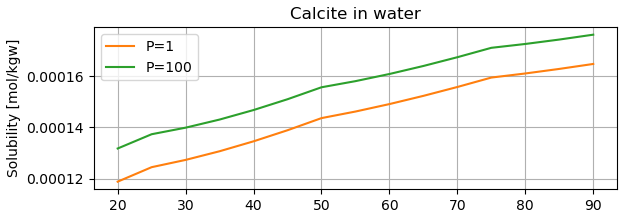
\includegraphics[height=2.2cm]{figures/chemical-equilibrium/calcite-solubility-water.png} \quad
	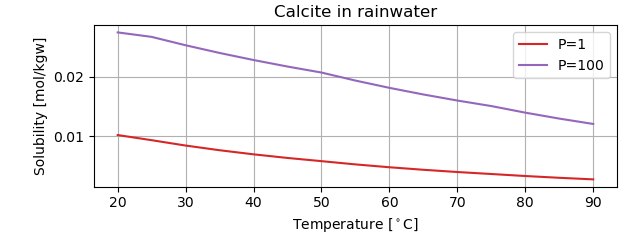
\includegraphics[height=2.2cm]{figures/chemical-equilibrium/calcite-solubility-rainwater.png}
	\caption*{\footnotesize Calcite solubility in water and rain water w.r.t. temperature.}
\end{figure}
\end{frame}

%
% --------------------------------------------------------------------------------------------------------------------%
% Calcite solubility example -- Stalagmites and stalactites
% --------------------------------------------------------------------------------------------------------------------%
%
\begin{frame}{Calcite solubility example, Stalagmites and stalactites}

The increased solubility of calcium carbonate in rainwater saturated with carbon dioxide is the {\bf driving force behind the erosion of limestone rocks}, leading to the formation over long periods of time of caverns, caves, stalagmites and stalactites.

\[\mathsf{CaCO_3(s) + CO_2(g) + H_2O(l) \rightleftharpoons Ca(HCO_3)_2(aq)}\]

\vskip -10pt
\begin{columns}[t]
\column{0.4\textwidth}
\vskip 10pt
$\rightarrow$ Rainwater meets with limestone to form a solution of calcium bicarbonate. \\[5pt]
$\leftarrow$ The bicarbonate-rich water drips from the ceiling of the cave and partially evaporates, leaving behind a calcium carbonate deposit.

\column{0.6\textwidth}

\begin{figure}\centering
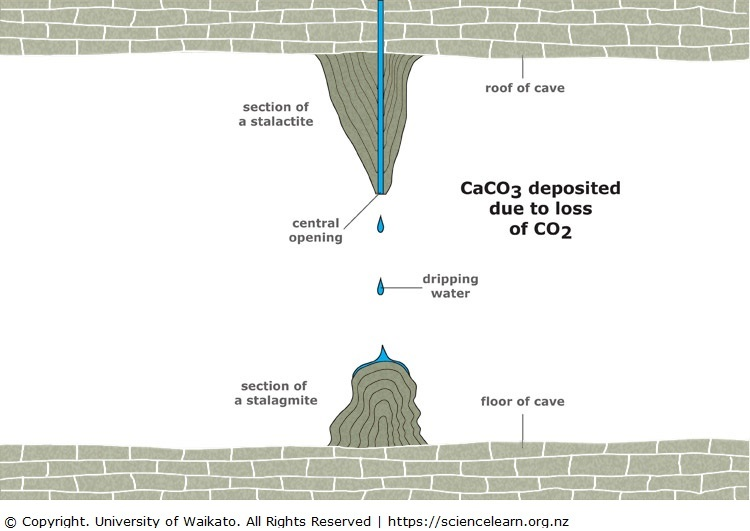
\includegraphics[width=0.6\textwidth]{figures/chemical-equilibrium/stalagmites-stalactities.jpg}
\caption*{\footnotesize
Diagram of cave showing formation of stalagmites and stalactites.}
\end{figure}

\end{columns}

\end{frame}
%
% --------------------------------------------------------------------------------------------------------------------%
% Calcite solubility example -- Limestone fizzing
% --------------------------------------------------------------------------------------------------------------------%
%
\begin{frame}{Calcite solubility example, Limestone fizzing}

\vskip 10pt
\begin{figure}
\centering
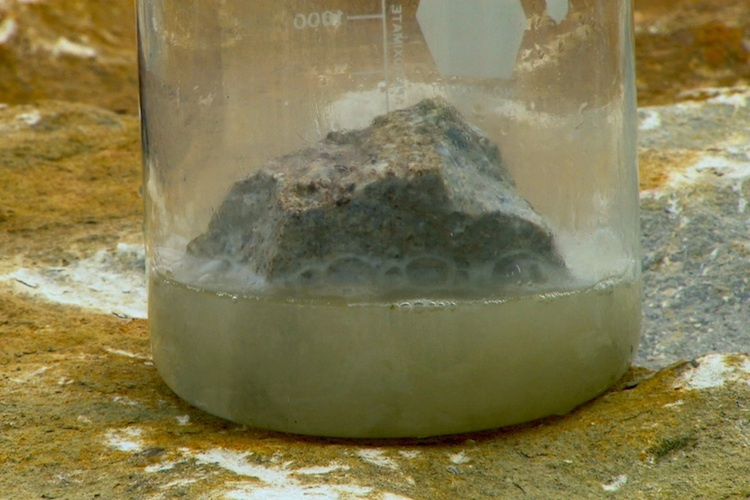
\includegraphics[width=0.6\textwidth]{figures/chemical-equilibrium/limestone-fizzing.jpg}
\caption*{Limestone fizzes when dilute acid is placed on its surface. The calcium carbonate present in the limestone is reacting with the acid to produce carbon dioxide gas.
}
% When dilute acid is placed on a sample of limestone rock, it fizzes. 
% The calcium carbonate present in the limestone is reacting with the acid to produce carbon dioxide gas.
\end{figure}

\end{frame}
%
% --------------------------------------------------------------------------------------------------------------------%
% Solubility of chlorargyrite, Example
% --------------------------------------------------------------------------------------------------------------------%
%
\begin{frame}{Solubility of chlorargyrite, Quiz}
	%
	\begin{itemize}
		\item Consider dissolution reaction of chlorargyrite 
		\[
		\mathsf{AgCl(s) \rightleftharpoons Ag^{+}(aq) + Cl^{-}(aq)}
		\]
		%
		\item  \alert{\bf Quiz}: What is solubility of AgCl(s) in 1 liter of water, where $K_{\sf sp} = 1.8 \cdot 10^{-10}$?
		\begin{center}
			\href{http://etc.ch/bv5y}{\textcolor{indigo(dye)}{\tt http://etc.ch/bv5y}} 
			\quad
			or 
			\quad
			
\includegraphics[height=0.2\columnwidth]{figures/chemical-equilibrium/poll.png}
		\end{center}
		\hiddenpause
		\item {\bf Answer}: 1 liter of water can dissolve $1.34 \cdot 10^{-5}$ mol/L of AgCl(s) at room temperature. \\
		%
		{\bf Note}: Compared with other types of salts, AgCl is also poorly soluble in water. \\
		In contrast, table salt NaCl has a higher $K_{\sf sp}$ and is, therefore, more soluble.
	\end{itemize}
\end{frame}		
%
\begin{frame}{Solubility of lead(II) chloride, Quiz}
	%
	\begin{itemize}
		\item Consider dissolution reaction of lead(II) chloride 
		\[
		\mathsf{PbCl_2(s) \rightleftharpoons Pb^{+}(aq) + 2\, Cl^{-}(aq)}
		\]
		% 
		with initial concentration of $\mathsf{PbCl_2(s)}$ = 0.1 mol.
		%
		\item  \alert{\bf Quiz}: What is solubility product $K_{\sf sp}$ of $\mathsf{PbCl2(s)}$ in 1 liter of water?
		\begin{center}
			\href{http://etc.ch/bv5y}{\textcolor{indigo(dye)}{\tt http://etc.ch/bv5y}} 
			\quad
			or 
			\quad
			
\includegraphics[height=0.3\columnwidth]{figures/chemical-equilibrium/poll.png}
		\end{center}
		\hiddenpause
		\item {\bf Answer}:  0.004.
	\end{itemize}
\end{frame}	
% \begin{frame}{Solubility of chlorargyrite, Quiz}
% 	%
% 	\begin{itemize}
% 		\item Consider dissolution reaction of chlorargyrite 
% 		\[
% 		\mathsf{AgCl(s) \rightleftharpoons Ag^{+}(aq) + Cl^{-}(aq)}
% 		\]
% 		%
% 		\item  \alert{\bf Quiz}: What is solubility of AgCl(s) in 1 liter of water, where $K_{\sf sp} = 1.8 \cdot 10^{-10}$?
% 		\begin{center}
% 			\href{http://etc.ch/bv5y}{\textcolor{indigo(dye)}{\tt http://etc.ch/bv5y}} 
% 			\quad
% 			or 
% 			\quad
% 			
\includegraphics[height=0.2\columnwidth]{figures/chemical-equilibrium/poll.png}
% 		\end{center}
% % 		\hiddenpause
% % 		\item {\bf Answer}: 1 liter of water can dissolve $1.34 \cdot 10^{-5}$ mol/L of AgCl(s) at room temperature. \\
% % 		%
% % 		{\bf Note}: Compared with other types of salts, AgCl is also poorly soluble in water. \\
% % 		In contrast, table salt NaCl has a higher $K_{\sf sp}$ and is, therefore, more soluble.
% 	\end{itemize}
% \end{frame}
% --------------------------------------------------------------------------------------------------------------------%
% Saturation index
% --------------------------------------------------------------------------------------------------------------------%
%
\begin{frame}{Saturation index}

The \alert{\textbf{saturation index}} indicates the saturation state of
a solution w.r.t. a other phase (e.g., mineral or gaseous), which is given by
%
\[
\boxed{ \mathsf{SI
= \log_{10} \frac{Q}{K_{\sf sp}} 
= \log_{10} \frac{IAP}{K_{\sf sp}}
= \log_{10} \frac{\prod_i [A_i]}{K_{\sf sp}}}},
\] 
where 
\begin{itemize}
\item Q is the \emph{ion activation product (IAP) / reaction quotient} of activities of the dissolved species (characteristic of non-equilibrium solution), 
and 
\item $\mathsf{K}_{\sf sp}$ is the \emph{solubility product / equilibrium constant}. 
\end{itemize}
%
\[
\mathrm{SI} \quad 
\begin{cases}
< 0& \mbox{solution is \textbf{undersaturated} $\Rightarrow$ the mineral may be dissolved }\\
= 0& \mbox{solution is \textbf{saturated} \qquad \; $\Rightarrow$ the mineral in equilibrium with solution}\\
> 0 & \mbox{solution is \textbf{supersaturated} $\Rightarrow$ the mineral may be precipitated}
\end{cases}
\]
%
%The solubility of a given solute can be determined with the solubility product.

\end{frame}
%
% --------------------------------------------------------------------------------------------------------------------%
% Saturation index, Example
% --------------------------------------------------------------------------------------------------------------------%
%
\begin{frame}{Saturation index, Exercise}
	
%	BaSO4(s)↽−−⇀Ba2+(aq)+SO2−4(aq)
%	Barium sulfate is used in medical imaging of the gastrointestinal tract. Solubility product of barium sulfate is 1.08×1e-10 at 25°C
%	
%	Will barium sulfate precipitate if 10.0 mL of 0.0020 M Na2SO4 is added to 100 mL of 3.2 × 10−4 M BaCl2? 
%	[Ba2+]=2.9×10−4 molal
%	[SO2−4]=1.8×10−4 molal
%	IAP = 5.2×10−8
%	IAP > Ksp: we predict that BaSO4 will precipitate when the two solutions are mixed. In fact, BaSO4 will continue to precipitate until the system reaches equilibrium, which occurs when 1.08×1e-10 is reached.

	\begin{itemize}
		\item Consider dissolution reaction of barium sulfate 
		%
		$\mathsf{BaSO_4(s) \rightleftharpoons Ba^{2+}(aq) + SO_4^{2-}(aq).}$
		%
		%
		\item Solubility product $K_{\sf sp}$ of barium sulfate is 1.08e-10 at 25 ${\rm ^\circ}$C.
		%
		\item  \alert{\bf Quiz}: What can be said about the water w.r.t. to barium sulfate if
		${\sf [Ba^{2+}}]=2.9 \cdot$ 1e-4 molal and 
		${\sf [SO_4^{2-}]}=1.8 \cdot$ 1e-4 molal
		%
		using formula
		%
		{\footnotesize
		\[
            \mathrm{SI} 
            = \log_{10} \frac{Q}{K_{\sf sp}} \quad 
            \begin{cases}
            < 0& \mbox{solution is \textbf{undersaturated} $\Rightarrow$ the mineral may be dissolved }\\
            = 0& \mbox{solution is \textbf{saturated} \qquad \:\,$\Rightarrow$ the mineral in equilibrium with solution}\\
            > 0 & \mbox{solution is \textbf{supersaturated} $\Rightarrow$ the mineral may be precipitated}
            \end{cases}
        \] 
        }
		%
		\begin{center}
			\href{http://etc.ch/bv5y}{\textcolor{indigo(dye)}{\tt http://etc.ch/bv5y}} 
			\quad
			or 
			\quad
			
\includegraphics[height=0.18\columnwidth]{figures/chemical-equilibrium/poll.png}
		\end{center}
		\hiddenpause
		\vskip 5pt
		\item {\bf Answer}: Water will be supersaturated with ${\sf BaSO_4(s)}$.
	\end{itemize}

\end{frame}
%
% --------------------------------------------------------------------------------------------------------------------%
% Saturation index, Demonstration
% --------------------------------------------------------------------------------------------------------------------%
%
\begin{frame}{Saturation index, Demonstration}
	\lcol
	\vskip -5pt
	\begin{itemize}
		\item Demonstration of gypsum/anhydrite solubility: 
		%
		Jupyter notebook tutorial 
		\href{https://github.com/mtsveta/reaktoro-v2-workshop/blob/main/tutorials/solubility/solubility-anhydrite.ipynb}{\textcolor{indigo(dye)}{\it Gypsum/anhydrite solubility in water}}.
		%
		\item Investigation on how saturated the Evian water with carbonates can be found in 
		Jupyter notebook tutorial \href{https://reaktoro.org/applications/miscellaneous/evian-water-analysis.html}{\textcolor{indigo(dye)}{\it Analysis of the Evian water}}.
		%
		\item Barite precipitation in the water flooding reactive transport example:
		%
		Jupyter notebook tutorial 
		\href{https://github.com/mtsveta/reaktoro-jupyter/blob/master/tutorial/rt.scaling.ipynb}{\textcolor{indigo(dye)}{\it One-dimensional reactive transport modeling of scaling (without oil)}}.
	\end{itemize}
	%
	\rcol
	\begin{figure}
		\centering
		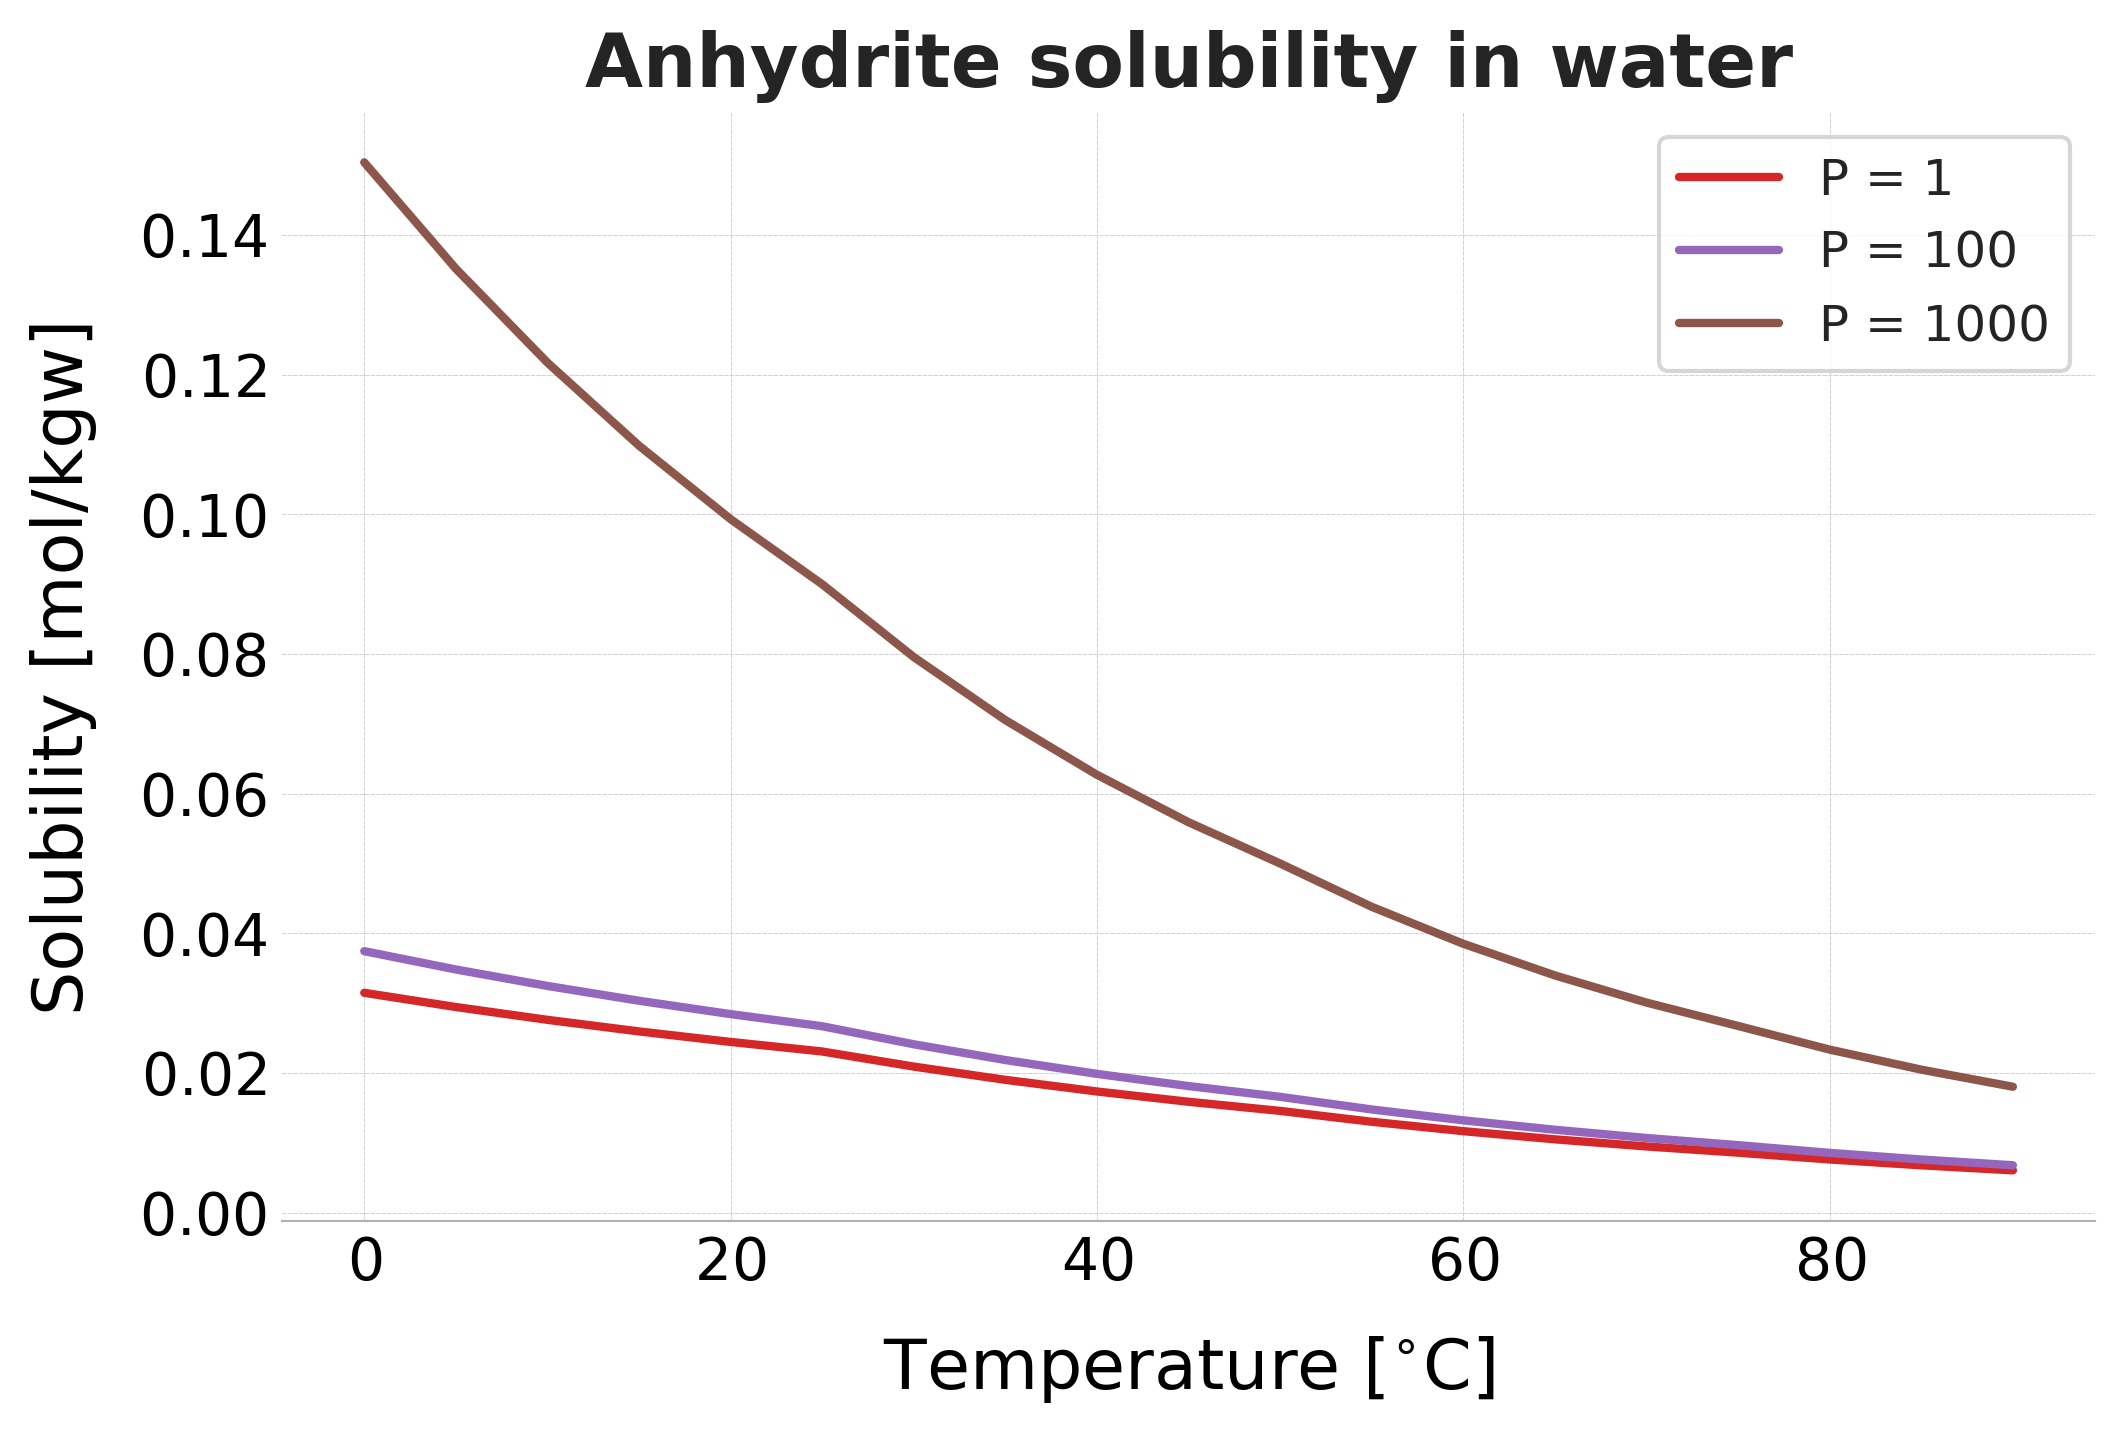
\includegraphics[width=0.75\columnwidth]{figures/chemical-equilibrium/anhydrite-solubility.png}
		%\caption{}
	\end{figure}
	\vskip -10pt
	\begin{figure}
		\centering
		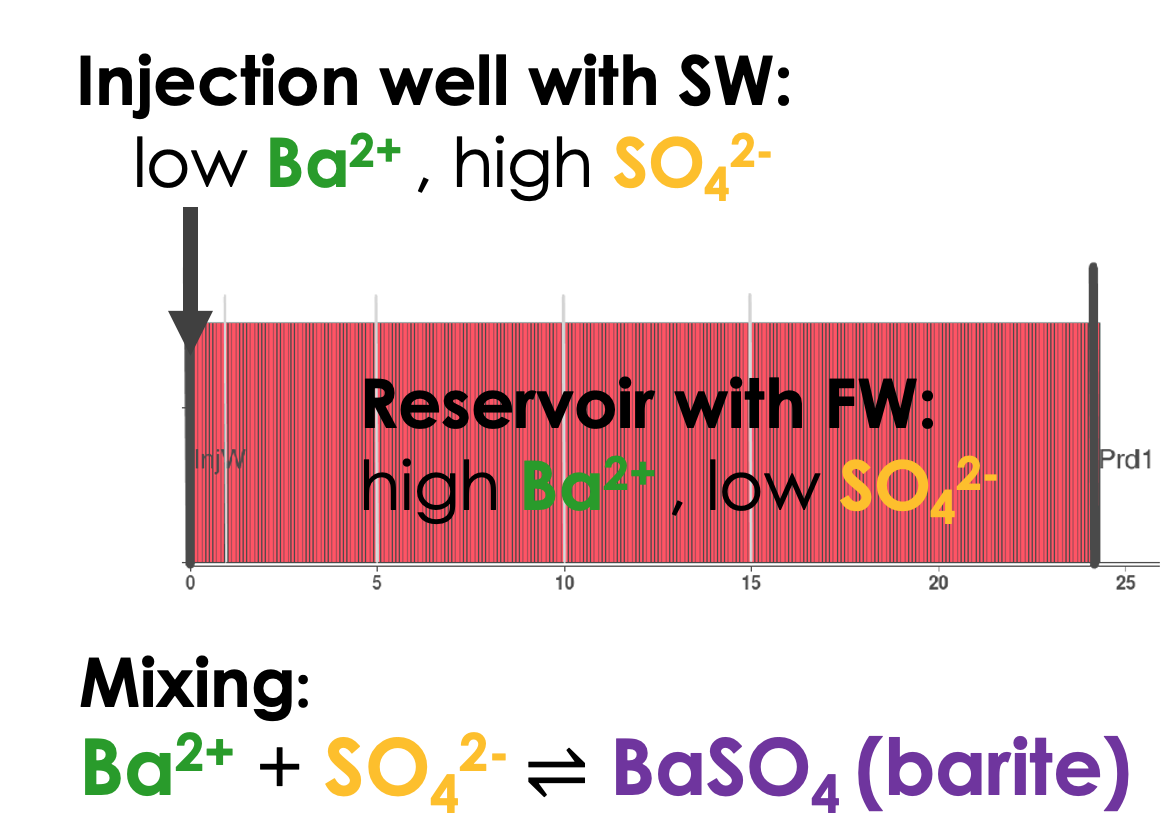
\includegraphics[width=0.7\columnwidth]{figures/chemical-equilibrium/barite-scaling.png}
		%\caption{}
	\end{figure}
	\ecol
	
	%\begin{itemize}
	%\item Demonstration of gypsum solubility: 
	%%
	%Jupyter notebook tutorial 
	%\href{}{\textcolor{indigo(dye)}{\it }}.
	%%
	%%
	%\item Barite precipitation in the water flooding RT example 
	%%
	%Jupyter notebook tutorial 
	%\href{}{\textcolor{indigo(dye)}{\it Calcite solubility in water and CO$_2$-saturated rainwater}}.
	%\end{itemize}
\end{frame}
	
%\begin{frame}{Barite scaling model illustration}
%	\centering
%	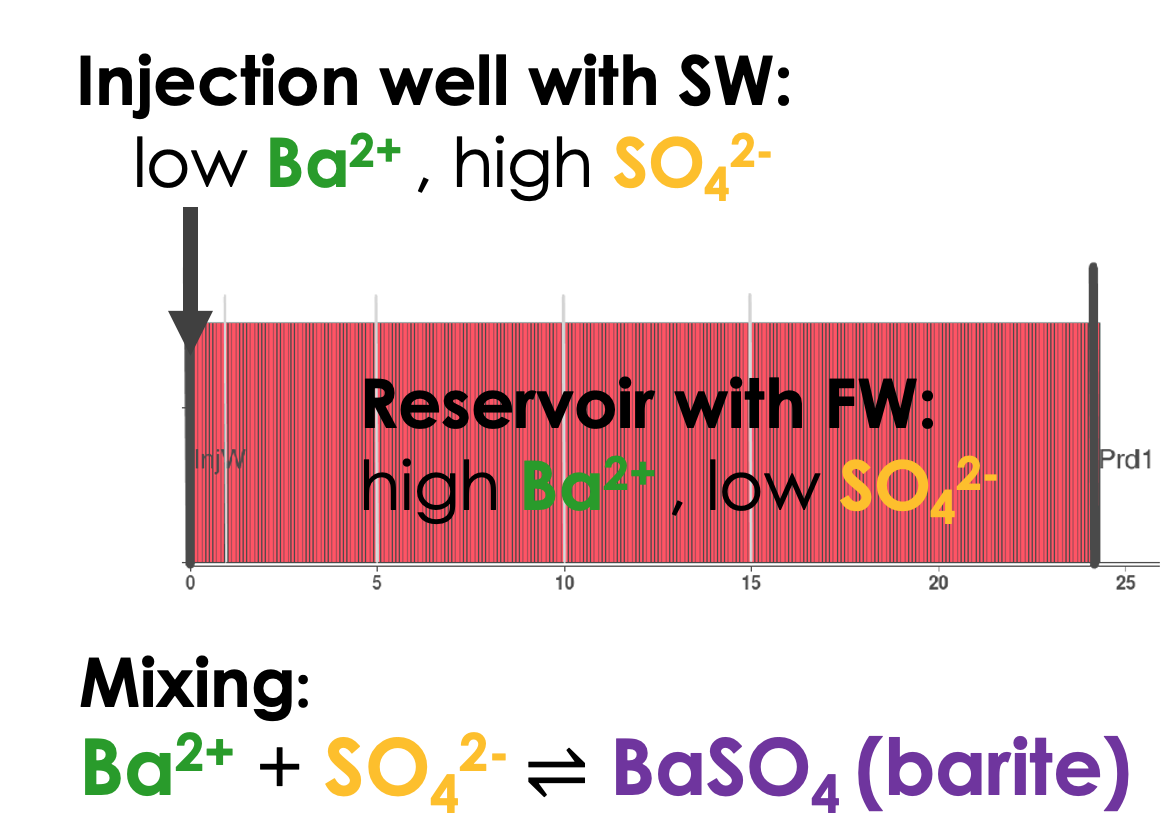
\includegraphics[width=0.75\columnwidth]{figures/chemical-equilibrium/barite-scaling.png}
%\end{frame}

%
%
% --------------------------------------------------------------------------------------------------------------------%
% Electroneutrality principle
% --------------------------------------------------------------------------------------------------------------------%
%
\begin{frame}{Electroneutrality principle}

\begin{itemize}
\item \alert{\textbf{Electroneutrality principle}} (Pauling, 1948) states that 
the ionic species in the electrolyte solution have equilibrium of charges on a macroscopic scale.
\pause
\item It can be expressed by the charge equilibrium between the species in solution
%
\[
\boxed {\sum_i Z_i m_i = 0,}
\]
%
where $Z_i$ are the ionic charges and 
$m_i$ are the molalities of species.
%
\pause 
\item \alert{\bf Example}: 
When mixing 0.1 molal of NaCl, it dissolves to 0.1 molal Na$^+$ and 0.1 molal Cl$^-$.

\end{itemize}
%
\end{frame}
%
% --------------------------------------------------------------------------------------------------------------------%
% Reduction/oxidation potential, pE
% --------------------------------------------------------------------------------------------------------------------%
%
\begin{frame}{Reduction/oxidation potential, pE}
\begin{itemize}
	\item  \alert{\textbf{Oxidation / reduction}} are the reactions, where species esquire / lose electrons, e.g., 
	%
	%\item Species in an aqueous solution can {\bf donate or accept electrons}, for example:
	%
	\[
	\mathsf{e^- + \tfrac{1}{4} \, O_2(aq) + H^+ = \tfrac{1}{2} \, H_2O.}
	\]
	\vskip -10pt
	%
	\pause
\item \alert{\textbf{Oxidation / reduction potential}} is a {\bf measure of the tendency} of a species to acquire/lose electrons from/to an electrode and thereby {\bf be reduced or oxidised}. 
%But such reaction is rather used as a {\bf half-reaction}. Additional half-reaction must be written to result into {\bf a charge-balanced equation}.
%. 
%
	\pause
\item The \alert{\textbf{reduction/oxidation potential}} $\mathsf{pE}$ is defined as
%
\[
\boxed{ \mathsf{pE} = - \log_{10} (a_{e^{\scalebox{0.75}[1.0]{-}}}) = -\tfrac{1}{n_e} \log \tfrac{Q^{\scalebox{0.75}[1.0]{-}}_e}{K^{\scalebox{0.75}[1.0]{-}}_e} }
\]
\vskip -5pt
%
where 
\begin{itemize}
	\item $K^{\scalebox{0.75}[1.0]{-}}_e \approx 25.5$ (at 25 \textdegree C), 
	\item $n_e$ is the number of consumed/generated electrons, and 
	\item $Q^{\scalebox{0.75}[1.0]{-}}_e$ is the product of the activities of the reaction. 
\end{itemize}
%
	\pause
\item A solution with a {\bf higher pE} /  {\bf lower pE} will have a tendency to {\bf gain electrons from} / {\bf lose electrons to} the new species.
%
\end{itemize}

\end{frame}
%
% --------------------------------------------------------------------------------------------------------------------%
% Hydrogen potential, pH
% --------------------------------------------------------------------------------------------------------------------%
%
\begin{frame}{Hydrogen potential, pH}

\begin{itemize}
	\item The \alert{\textbf{pH}} of a solution is an indication of the \textbf{tendency} of the solution \textbf{to donate hydrogen ions}
	or measure of the \textbf{relative amount of free hydrogen ions} in the solution. 
	%
		\pause
	
\item The \alert{\textbf{hydrogen potential}} $\mathsf{pH}$ is defined as
%
\[
\boxed{ 
\mathsf{pH} = - \log_{10} (a_{\mathsf{H^+}}) = - \log_{10} ([H^+]). 
}
\]
%
\vskip -10pt
	\pause
\item $\mathsf{pH}$ is a measure of how \textbf{acidic/basic} solution is in the scale from 0 till 14: 
%
%\begin{alignat*}{2}
%\mathsf{pH} < 7: & \qquad \mbox{solution is \textbf{acidic}}\\
%\mathsf{pH} = 7: & \qquad \mbox{solution is \textbf{neutral}}\\
%\mathsf{pH} > 7: & \qquad  \mbox{solution is \textbf{alkali/base}}
%\end{alignat*}
%
%\[
%\mathsf{pH} < 7: \; \mbox{solution is \textbf{acidic}} \qquad
%\mathsf{pH} = 7: \; \mbox{solution is \textbf{neutral}} \qquad
%\mathsf{pH} > 7: \; \mbox{solution is \textbf{alkali/base}}
%\]
\end{itemize}
\begin{figure}
\centering
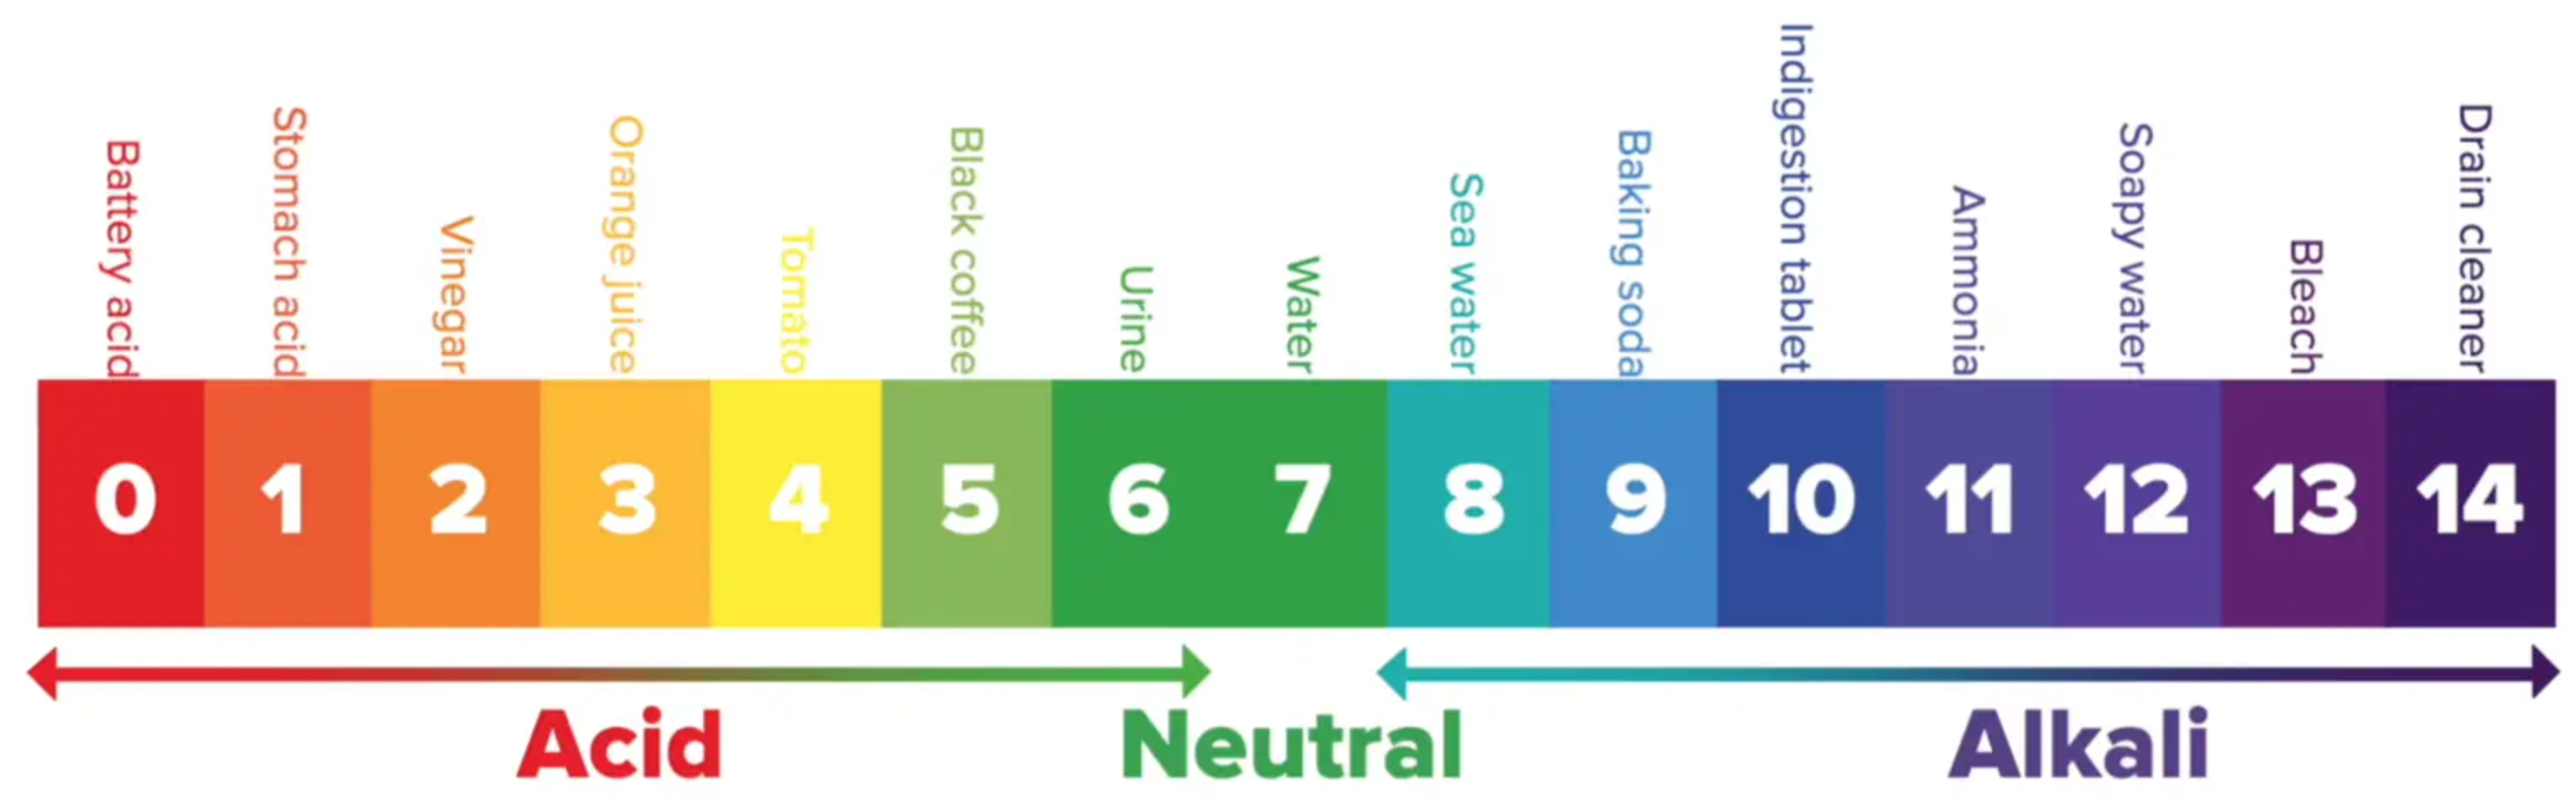
\includegraphics[width=0.9\columnwidth]{figures/chemical-equilibrium/ph-scale.png}
\end{figure}
\end{frame}

\begin{frame}{Examples with negative pH}

%$\bullet$ pH can be defined and measured below zero. \\
$\bullet$ The \alert{\bf waters of such low pH exist in nature} with the following sources of extreme acidity: \\
\quad - {\bf magmatic gases} %that contribute HCl, HF, and
%$\mathsf{H_2SO_4}$ to 
in vents, fumaroles, crater lakes, and hot springs in active geothermal areas \\
\quad - the {\bf oxidation of pyrite} which produces sulfuric acid. \\ 

\begin{columns}[t]
\column{0.3\textwidth}
\begin{figure}
\centering
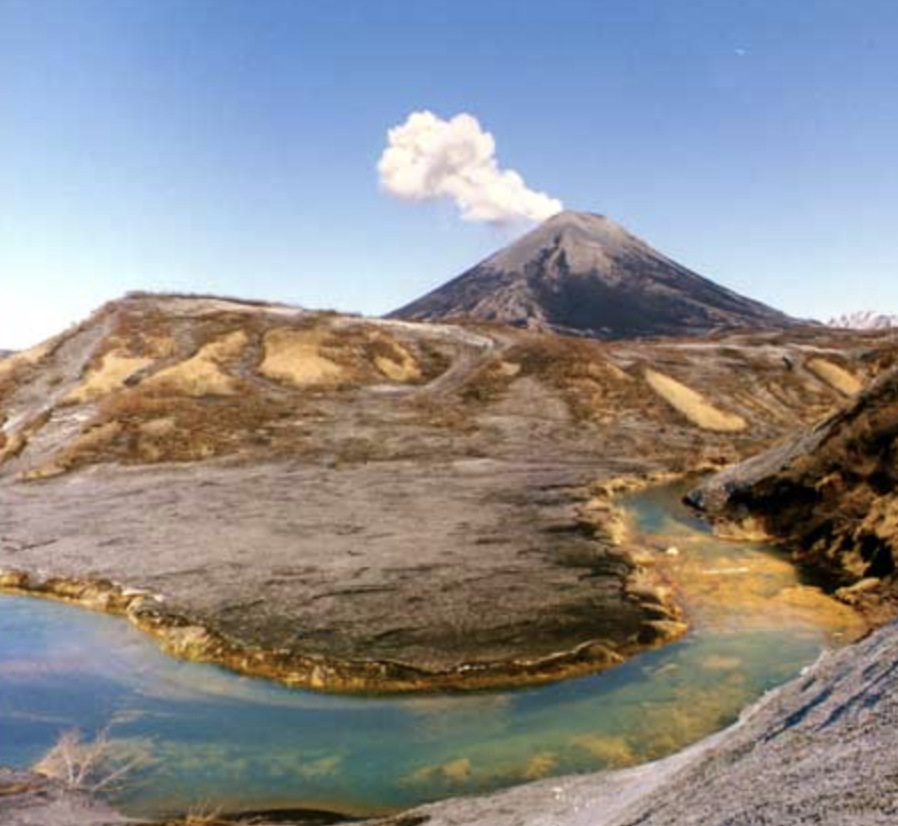
\includegraphics[width=0.9\columnwidth]{figures/chemical-equilibrium/ebeko.png}
\caption*{The $\mathsf{HCl-H_2SO_4}$ hot springs 
near Ebeko volcano with {\bf pH as low as -1.7}.}
\end{figure}
\column{0.3\textwidth}
\begin{figure}
\centering
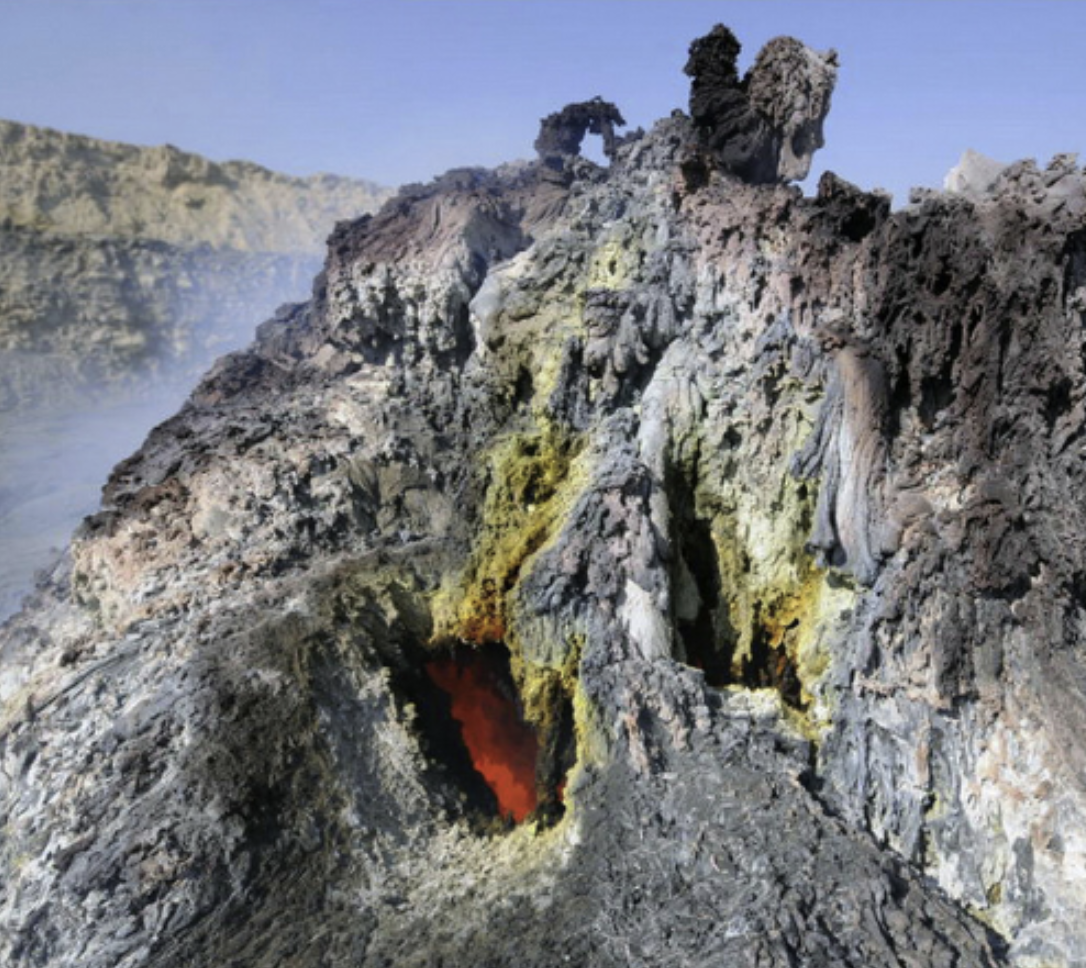
\includegraphics[width=0.9\columnwidth]{figures/chemical-equilibrium/kilauea.png}
\caption*{The HCl-HF fumarolic condensates from Kilauea Iki with {\bf pH = -0.3}.}
\end{figure}
\column{0.3\textwidth}
\centering
\begin{figure}
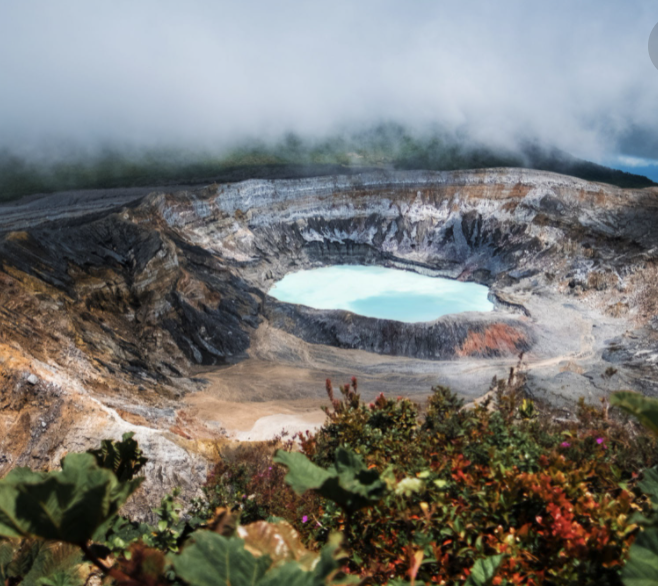
\includegraphics[width=0.9\columnwidth]{figures/chemical-equilibrium/poas.png}
\caption*{The lake waters from Poas crater, Costa Rica with {\bf pH of -0.89}.}
\end{figure}
\end{columns}

% \footnotesize
% \begin{columns}[t]\column{0.7\textwidth}
% \vskip 10pt
% The most acidic pH values reported for environmental
% samples: 
% \begin{itemize}
% \item the $\mathsf{HCl-H_2SO_4}$ hot springs
% near Ebeko volcano with estimated {\bf pH as low as -1.7}
% %
% \pause
% \vskip 10pt
% \pause 
% \item the HCl-HF fumarolic condensates from Kilauea Iki estimated to have a pH = -0.3
% %
% \pause
% \vskip 10pt
% \pause 
% \item the lake waters from Poas crater, Costa Rica with an estimated pH of -0.89.
% \end{itemize}
% %
% \column{0.3\textwidth}
% \vskip -10pt
% \begin{figure}
% \centering
% 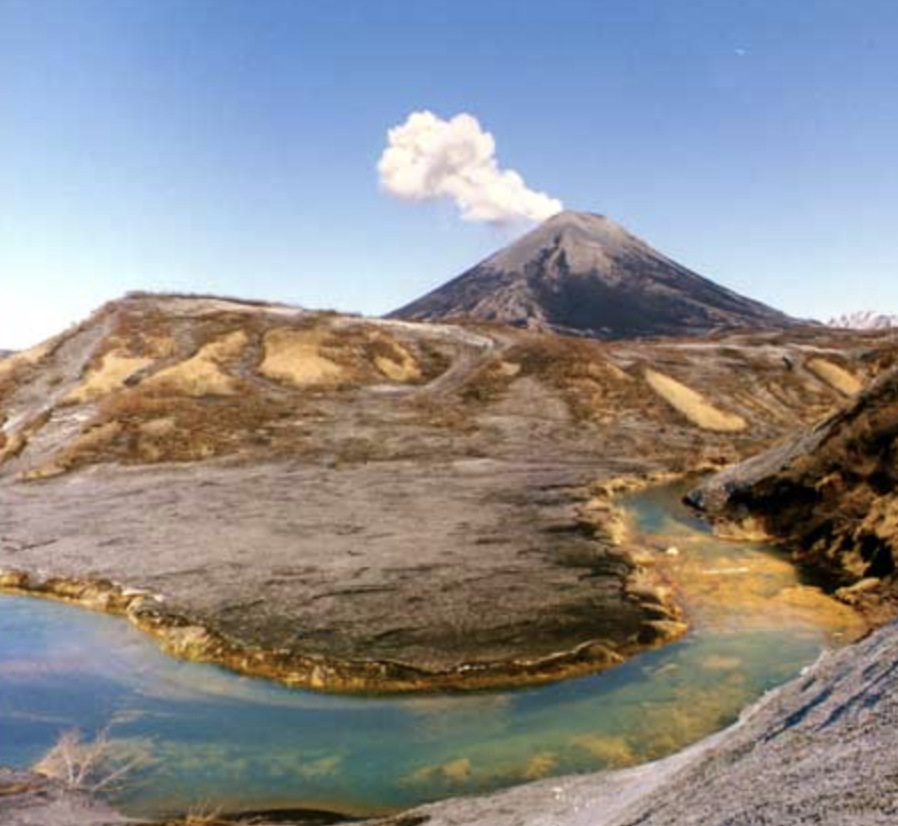
\includegraphics[width=0.6\columnwidth]{figures/chemical-equilibrium/ebeko.png}
% %\caption{}
% \end{figure}
% \vskip -10pt
% \begin{figure}
% \centering
% 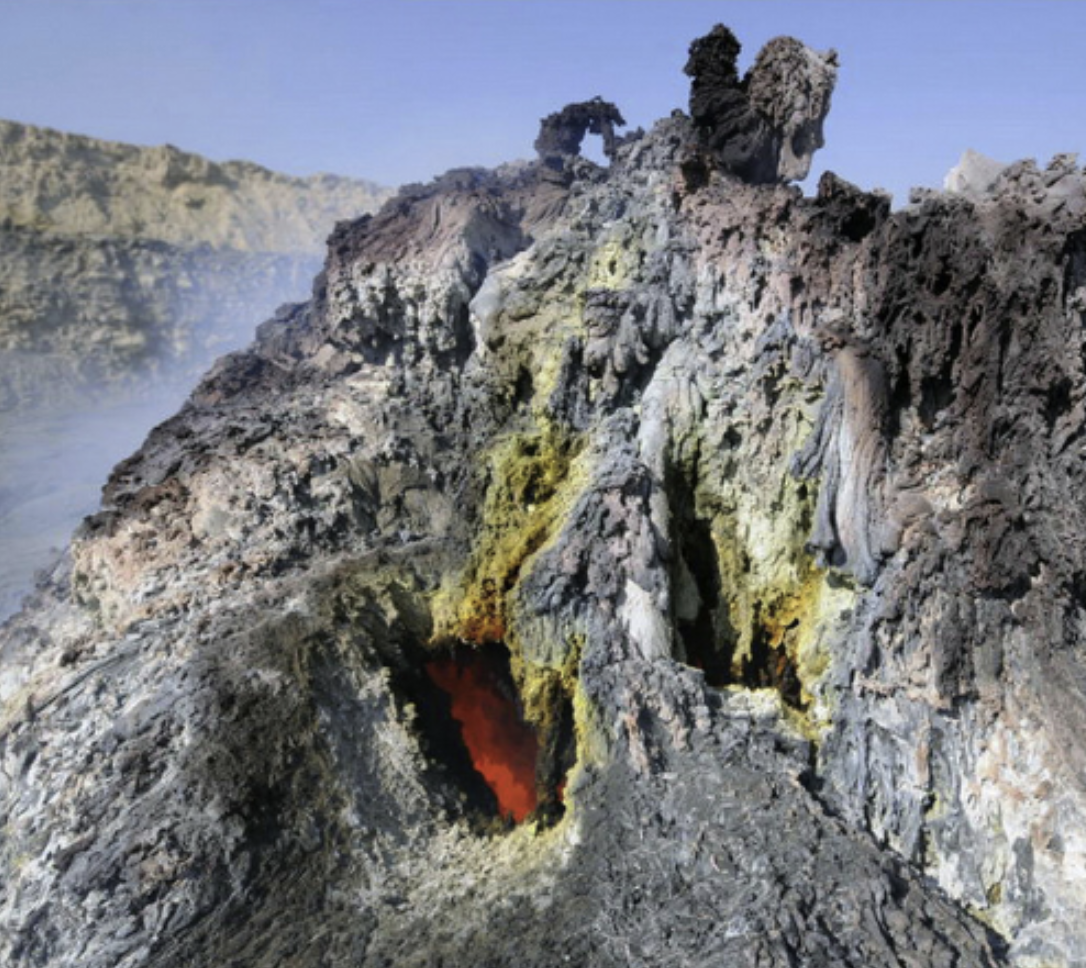
\includegraphics[width=0.6\columnwidth]{figures/chemical-equilibrium/kilauea.png}
% %\caption{}
% \end{figure}
% \vskip -10pt
% \begin{figure}
% \centering
% 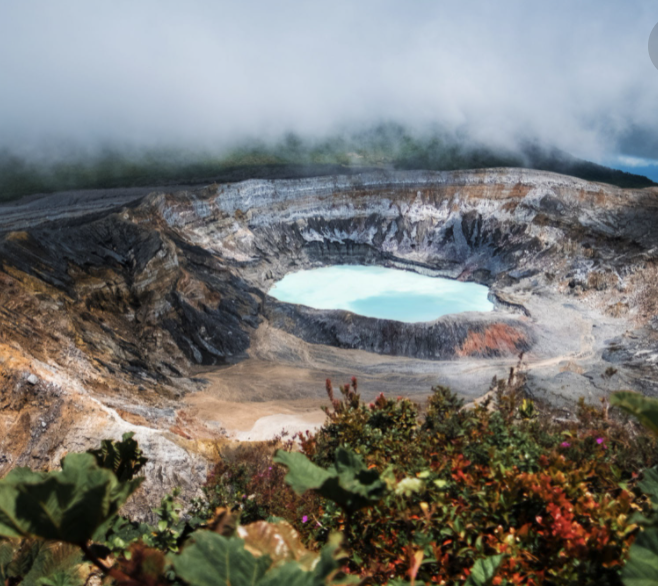
\includegraphics[width=0.6\columnwidth]{figures/chemical-equilibrium/poas.png}
% %\caption{}
% \end{figure}

% \end{columns}

\end{frame}
%
% --------------------------------------------------------------------------------------------------------------------%
% Saturation index, Example
% --------------------------------------------------------------------------------------------------------------------%
%
\begin{frame}{pH, Quiz \: i}

\alert{\bf Quiz}: which of the following properties indicates a low pH of hot springs near the Ebeko volcano in the Pacific Ocean?
%
\vskip 10pt
\begin{center}
	\href{http://etc.ch/bv5y}{\textcolor{indigo(dye)}{\tt http://etc.ch/bv5y}} 
	\quad
	or 
	\quad
	\includegraphics[height=0.2\columnwidth]{figures/chemical-equilibrium/poll.png}
\end{center}
\vskip 10pt
\hiddenpause
{\bf Answer}: it has high concentrations of $\mathsf{H^+}$ ions.
\end{frame}

\begin{frame}{pH, Quiz \: ii}
	\small
	\begin{itemize}
		\item We have completely dissolved HCl in the 300 ml of water  
		%
		$\mathsf{HCl(aq) \rightleftharpoons H^+(aq) + Cl^-(aq)}$
		%
		%
		 and it produced the solution with pH = 1. 
		%
		\pause
		\item {\bf Hint 1}: let the concentration $[\mathsf{H^+}]$ (measured in mol/L) and $a_{\mathsf{H^+}}$ be the same (i.e., activity is considered as effective concentration). 
		%
		\item {\bf Hint 2}: $m_{\mathsf{HCl}} = M_{\mathsf{HCl}}  \cdot n_{\mathsf{HCl}},$ 
		%
		where $m$ is the mass of species (in kg), 
		$M$ is the molar mass (in kg / mol), and 
		$n$ is the molar amount (in mol). 
		%
		\item {\bf Hint 3}: molar amount of $M_{\mathsf{HCl}} = $ 36.458 g/mol .
		%
		\pause
		\item  \alert{\bf Quiz}: What was the mass of dissolved HCl?
		%
		\begin{center}
			\href{http://etc.ch/bv5y}{\textcolor{indigo(dye)}{\tt http://etc.ch/bv5y}} 
			\quad
			or 
			\quad
			\includegraphics[height=0.13\columnwidth]{figures/chemical-equilibrium/poll.png}
		\end{center}
 		\hiddenpause
 		\item {\bf Answer}: 
        1) find concentration of hydrogen ions: 
        $\mathsf{[H^+] = 10^{-pH}}$ = 0.1 mol/L \\
        2) amount of hydrogen per 0.3 L: 
        $\mathsf{n(H^+) = [H^+] mol/L \cdot V_{H_2O}}$ 
        = 0.1 $\cdot$ 0.3 = 0.03 mol \\
        3) mass of HCl: 
        $m_{\mathsf{HCl}}$ = 0.03 mol $\cdot$ 36.458 g/mol = 1.09374 
	\end{itemize}
\end{frame}
% --------------------------------------------------------------------------------------------------------------------%
% pH, Examples i
% --------------------------------------------------------------------------------------------------------------------%
%
\begin{frame}{pH, Examples \, i}
	
	\lcol
	\vskip -5pt
	\begin{itemize}
		\item Too high or too low pH effect aquatic / fish life (see explanation of \href{https://www.sciencelearn.org.nz/videos/1961-ph}{\textcolor{indigo(dye)}{\it Dr E. Ryan, Waikato Regional Council}}). 
		\pause
		\item 
	Large \alert{\textbf{algae blooms}} can affect the pH as they photosynthesise: 
	\begin{itemize}
		\item during the day that \textbf{drives the pH down} and 
		\item at night when they respire, it \textbf{drives the pH up}.
		%
	\end{itemize}
	%
	\alert{\textbf{The results}}: \textbf{huge pH fluctuations} in water, which can affect fish quite negatively. 
	\end{itemize}
	%
	\rcol
	%\vskip -30pt
	\begin{figure}
		\centering
		\includegraphics[width=0.85\columnwidth]{figures/chemical-equilibrium/toxic_algae_bloom_lake_erie.jpg}
		\caption{\small The worst algae bloom that Lake Erie has experienced in decades resulting from the record torrential spring rains washed fertilizer into the lake, promoting the growth of microcystin-producing cyanobacteria blooms.}
	\end{figure}

	\ecol
	
\end{frame}
%
% --------------------------------------------------------------------------------------------------------------------%
% pH, Examples ii
% --------------------------------------------------------------------------------------------------------------------%
%
\begin{frame}{pH, Examples \, ii}
\footnotesize
\lcol

\begin{itemize}
\item $\mathsf{CO_2}$ added to the seawater influences the $\mathsf{pH}$ according to the reaction
%
\[
\mathsf{CO_2(g) + H_2O(l) = H^+ + HCO_3^-.}
\]
% 
See tutorial \href{https://reaktoro.org/applications/miscellaneous/ph-dependence-on-co2-addition-in-seawater.html}{\textcolor{indigo(dye)}{\it Dependence of the pH on the $\mathsf{CO_2(g)}$ amount in seawater}}.
%
\pause
\vskip 10pt
\pause
\item Adding HCl into water increases free $\mathsf{H^+}$ ions and decreases pH according to the reaction 
%
\[
\mathsf{HCl(aq) + H_2O(l) = H_3O^+ + Cl^-,}
\]
%
whereas 
%Water and HCl combine to form \textbf{hydrochloric acid} ($\mathsf{H_3O^+}$ and $\mathsf{Cl^-}$):
%
%\[
%\mathsf{HCl(aq) + H_2O(l) = H_3O^+ + Cl^-.}
%\]
%
adding ammonia \textbf{removes} $\mathsf{H^+}$ from water and increases it to produce ammonium and hydroxide, i.e., 
%to produce ammonium and hydroxide:
%
\[
\mathsf{NH_3 + H_2O = NH_4^+ + OH^-.}
\]
%
%
%By adding acid, we decrease the $\mathsf{pH}$ of water
%%
%\[
%\mathsf{HCl(aq) + H_2O(l) = 2\, H^+ + HO^- + Cl^-.}
%\]
% 
See tutorial \href{https://reaktoro.org/applications/miscellaneous/ph-dependence-on-contaminants-in-water.html}{\textcolor{indigo(dye)}{\it Dependence of the pH on added contaminant in water}}.

\end{itemize}
%
\rcol
\begin{figure}
\centering
\includegraphics[width=0.82\columnwidth]{figures/chemical-equilibrium/ph-dependence-on-co2-amount-in-seawater.png}
%\caption{}
\end{figure}
\vskip -10pt
\begin{figure}
\centering
\includegraphics[width=0.82\columnwidth]{figures/chemical-equilibrium/ph-dependence-on-contaminants-in-water.png}
%\caption{}
\end{figure}
\ecol

\end{frame}




%\section{Thermodynamic models of aqueous, gaseous, and mineral phases}
%
% --------------------------------------------------------------------------------------------------------------------%
% Activities - the effective concentrations of the species
% --------------------------------------------------------------------------------------------------------------------%
%
\begin{frame}{Activities -- the effective concentrations of the species}
\begin{itemize}
\item Let $c_{i}$ denote concentration of species $i$ (\textbf{Note}: sometime in literature it is denoted by $[i]$, 
but i$[i] \neq n_i$).
\pause
\item If we would use $c_{i}$ instead of activities $a_{i}$ to calculate the chemical potentials, then
\[
\mu_{i}=\mu_{i}^{\circ}+RT\ln a_{i} \qquad\text{can be reformulated by} \qquad \mu_{i}=\mu_{i}^{\circ}+RT\ln(c_{i}/c_{i}^{\circ})
\]
where $c_{i}^{\circ}$ is a reference concentration
%
\pause
\item \alert{\textbf{But!}} This simplification provides \textbf{accurate predictions only in some limited cases}:
%
\begin{itemize}
\item gases at low pressures and high temperatures \alert{(close to ideal gas behavior)}
\item very dilute electrolyte solutions \alert{(close to ideal solution behavior)}
\end{itemize}
\end{itemize}
\end{frame}
%
% --------------------------------------------------------------------------------------------------------------------%
% Activities -- corrected species “concentrations” in non-ideal mixtures
% --------------------------------------------------------------------------------------------------------------------%
%
\begin{frame}{Activities -- corrected species “concentrations” in non-ideal mixtures}
\begin{itemize}
\item Because of the \textbf{non-ideal behavior of the mixtures}, the concentrations
of the species must be corrected:
%
\[
a_{i}=\gamma_{i}(T,P,c) \tfrac{c_i}{c_i^0},
\]
%
where $\gamma_{i}$ is an \alert{\textbf{activity coefficient}}, a function
of $(T,P,c)$, with $c$ denoting a {\bf vector of concentrations of all species in the solution}. 
\pause
\item $\gamma_i$ depends on the whole vector $c$, not just its $i$th component $c_i$.
\pause
\item To calculate $\gamma_{i}$, there are different (theoretical) \alert{\textbf{activity models}}:
\begin{itemize}
\item Davies equation,
\item Debye-H\"uckel equation,
%\item HKF
\item Pitzer equations, etc.
\end{itemize}
\end{itemize}
\end{frame}
%
% --------------------------------------------------------------------------------------------------------------------%
% Aqueous phase
% --------------------------------------------------------------------------------------------------------------------%
\subsection{Aqueous phase}
%
%{\begin{frame}{}
%\centering
%\Large
%\textbf{Aqueous phase}
%\end{frame}}
%
% --------------------------------------------------------------------------------------------------------------------%
% Activities of aqueous solute species
% --------------------------------------------------------------------------------------------------------------------%
%
\begin{frame}{Activities of aqueous solute species}
%
\lcol
\begin{itemize}
\item The \alert{\textbf{activity of aqueous solute species}}, such as H$^{+}$(aq), HCO$_{3}^{-}$(aq),
CO$_{2}$(aq), is defined as:
\[
a_{i}=\gamma_{i}m_{i},
\]
where:
\begin{itemize}
\item $\gamma_{i}$ is the \textbf{activity coefficient} of solute species
$i$; and
\item $m_{i}$ is the \textbf{molality} of solute species $i$.	
\end{itemize}
\end{itemize}
\rcol
\pause
\begin{itemize}
\item The  \alert{\textbf{molality}} $m_{i}$ of the $i$th aqueous species is form of describing concentrations and is defined as follows:
\[
m_{i}=\tfrac{n_{i}}{\text{mass of solvent species H\ensuremath{_{2}}O(aq)}},
\]
or equivalently:
\begin{alignat*}{2}
m_{i} & =  \tfrac{n_{i}}{\mbox{molar mass}(\mathsf{H_{2}O\text{(aq)}}) \cdot n_{\mathsf{H_{2}O\text{(aq)}}}} \\
         & =  \tfrac{n_{i}}{18.01528 \cdot 10^{-3} \cdot  n_{\mathsf{H_{2}O\text{(aq)}}}} \\
         & = 55.508\tfrac{n_{i}}{n_{\mathsf{H_{2}O\text{(aq)}}}}.
\end{alignat*}
\end{itemize}
\ecol
\end{frame}
%
% --------------------------------------------------------------------------------------------------------------------%
% Molarity vs. molality
% --------------------------------------------------------------------------------------------------------------------%
%
\begin{frame}{Molarity vs. molality}
%
\lcol
\vskip 20pt
\begin{itemize}
\item The \textbf{molarity} $c_{i}$ of the $i$th species is:
\begin{alignat*}{2}
c_{i} & = \tfrac{n_{i}}{\text{volume of solvent species H\ensuremath{_{2}}O(aq)}} \\
	& = \tfrac{n_{i} \cdot \rho_{\sf H{_{2}}O(aq)}}{\text{mass of solvent species H\ensuremath{_{2}}O(aq)}},
\end{alignat*}
where $\rho_{\sf H{_{2}}O(aq)}$ is \textbf{water density} at given $T$ and $P$.
\item Measured in units of {\bf \alert{molar} = mol/L (or mol/Lw or  $10^3$mol/m$^3$)}. 
\end{itemize}
\rcol
\begin{itemize}
\item The \textbf{molality} $m_{i}$ of the $i$th species is:
\[
m_{i}=\tfrac{n_{i}}{\text{mass of solvent species H\ensuremath{_{2}}O(aq)}}.
\]
\item Measured in units of {\bf \alert{molal} = mol/kg (or mol/kgw)}. 
\end{itemize}
\ecol
\end{frame}
%
% --------------------------------------------------------------------------------------------------------------------%
% Ionic strength of aqueous solutions
% --------------------------------------------------------------------------------------------------------------------%
%
\begin{frame}{Ionic strength of aqueous solutions}
%
\lcol
\begin{itemize}
\item Most activity models for aqueous solutions depends on the  \alert{\textbf{ionic strength}}:
\[
\boxed{I=\tfrac{1}{2}\sum_{i=1}^{\text{solutes}}m_{i}Z_{i}^{2}},
\]
where:
\begin{itemize}
\item $m_{i}$ is the \textbf{molality} of species $i$; and
\item $Z_{i}$ is the \textbf{electric charge }of species $i$.
\end{itemize}
\pause
\item $I$ is a measure (in molal) of \emph{how much concentrated is the solution with ionic
species}, 
\item \textbf{Note}: \alert{Neutral species} play no role in $I$, just the ions.
\end{itemize}
\rcol
\begin{itemize}
	\pause
\item \alert{\textbf{Question:}} What is the ionic strength $I$ of a solution obtained
by mixing 1 kg of H$_{2}$O and:
\begin{itemize}
\item[a)] 2 mol of NaCl?
\item[b)] 1 mol of CaCl$_{2}$?
\end{itemize}
\vskip 5pt
\begin{center}
\href{http://etc.ch/qjLF}{\textcolor{indigo(dye)}{\tt http://etc.ch/qjLFhttp://etc.ch/qjLF}} or 
\includegraphics[height=0.45\columnwidth]{figures/activity-models/poll-ionic-strength.png}
\end{center}
\hiddenpause
\item \textbf{Answer:}
a) 2 molal, 
b) 3 molal
\end{itemize}
\ecol
\end{frame}
%
% --------------------------------------------------------------------------------------------------------------------%
% Calculating species molalities and ionic strength, Exercise
% --------------------------------------------------------------------------------------------------------------------%
%
\begin{frame}{Calculating species molalities and ionic strength,  Exercise}

\lcol
\begin{center}
\begin{tabular}{ccc}
\toprule 
\textbf{Index} & \textbf{Species} & \textbf{Amount (mol)}\tabularnewline
\midrule
1 & \textrm{$\mathsf{H_{2}O(aq)}$} & 55.4551\tabularnewline
2 & \textrm{$\mathsf{H^{+}(aq)}$} & $1.23485\cdot10^{-4}$\tabularnewline
3 & \textrm{$\mathsf{OH^{-}(aq)}$} & $8.39739\cdot10^{-11}$\tabularnewline
4 & \textrm{$\mathsf{Na^{+}(aq)}$} & 0.92\tabularnewline
5 & \textrm{$\mathsf{Cl^{-}(aq)}$} & 0.92\tabularnewline
6 & \textrm{$\mathsf{CO_{3}^{-2}(aq)}$} & $4.93648\cdot10^{-11}$\tabularnewline
7 & \textrm{$\mathsf{HCO_{3}^{-}(aq)}$} & $1.23484\cdot10^{-4}$\tabularnewline
8 & \textrm{$\mathsf{CO_{2}(aq)}$} & 0.032861\tabularnewline
9 & \textrm{$\mathsf{CO_{2}(g)}$} & 1.96702\tabularnewline
10 & H$_{2}$O(g) & 0.0531732\tabularnewline
\bottomrule
\end{tabular}
\par\end{center}

\rcol

\textbf{Exercise:}
\begin{itemize}
\item Calculate the mass $M_{w}$ of solvent water H$_{2}$O(aq) (in kg).
Use 18.0154 g/mol as an approximated molar mass of water.
\item Calculate the molalities $m_{i}$ of the aqueous solute species (in
molal).
\item Calculate the ionic strength $I$ of aqueous solution (in molal).
\end{itemize}

\ecol
\end{frame}
%
% --------------------------------------------------------------------------------------------------------------------%
% Calculating species molalities and ionic strength using Python
% --------------------------------------------------------------------------------------------------------------------%
%
\begin{frame}[fragile, allowframebreaks]{Calculating species molalities and ionic strength using Python}

\lstinputlisting[language=Python, caption=Calculating species molalities and ionic strength using Python]{python-files/species-molalities-and-ionic-strength-with-blanks.py}

\textbf{Source code}: \href{https://polybox.ethz.ch/index.php/s/xmvAZqB9bcGvEz3}{\textcolor{indigo(dye)}{\it polybox}}.

\end{frame}
%
% --------------------------------------------------------------------------------------------------------------------%
% Calculating species molalities and ionic strength using Python -- Output
% --------------------------------------------------------------------------------------------------------------------%
%
\begin{frame}[fragile]{Calculating species molalities and ionic strength using Python -- Output}

\begin{lstlisting}[language=Python, caption=Calculating species molalities and ionic strength using Python -- Output]
Ionic strength of solution is 0.921001 molal.
Molality of H2O(aq)  is 5.5508e+01 molal.
Molality of H+       is 1.2360e-04 molal.
Molality of OH-      is 8.4054e-11 molal.
Molality of Na+      is 9.2088e-01 molal.
Molality of Cl-      is 9.2088e-01 molal.
Molality of CO3--    is 4.9412e-11 molal.
Molality of HCO3-    is 1.2360e-04 molal.
Molality of CO2(aq)  is 3.2892e-02 molal.
\end{lstlisting}

\textbf{Answer}: To check the correctness of gaps in the code, use the  \href{https://polybox.ethz.ch/index.php/s/o0tt6lPtd8TBhoG}{\textcolor{indigo(dye)}{\it source code}}.

\end{frame}
%
\subsubsection{Activity coefficient model for aqueous ionic species, Davies model}
%
% --------------------------------------------------------------------------------------------------------------------%
% Activity coefficient model for aqueous ionic species: Davies model
% --------------------------------------------------------------------------------------------------------------------%
%
\begin{frame}{Activity coefficient of aqueous species, Structure}
\begin{figure}
\centering{}\includegraphics[height=0.9\textheight]{figures/activity-models/activity-aqueous-species-1}
\end{figure}


\end{frame}

\begin{frame}{Activity coefficient of aqueous ionic species, Davies model}
\begin{itemize}[<+->]
\item The \alert{\textbf{Davies activity coefficient model} } calculates $\gamma_{i}$
using:
\[
\boxed{\log_{10}\gamma_{i}=-A_{\gamma}Z_{i}^{2}\left(\dfrac{\sqrt{I}}{1+\sqrt{I}}-0.3I\right),}
\]
where $A_{\gamma}$ is the \textbf{Debye–Hückel parameter} defined as
\[
A_{\gamma}=1.824928\cdot10^{6}\rho_{\mathsf{H_{2}O}}^{1/2}(\epsilon_{\mathsf{H_{2}O}}T)^{-3/2},
\]
%
where $\rho_{\mathsf{H_{2}O}}$ and $\epsilon_{\mathsf{H_{2}O}}$
are the \textbf{density} and \textbf{dielectric constant of pure water} resp. 
\item For 25~°C and 1~bar, $A_{\gamma}=0.5095$.
\item \textbf{Limitations of the model}: 
It is accurate for $I$ is in the range 0.1–0.7 molal, which is equivalent to 1 kg of water mixed with 5.8–40.9 grams of NaCl (0.5-4 teaspoons of table salt).
\end{itemize}
\end{frame}
%
% --------------------------------------------------------------------------------------------------------------------%
% Activity coefficient model for aqueous ionic species: Davies model 
% --------------------------------------------------------------------------------------------------------------------%
%
\begin{frame}{Activity coefficient of aqueous ionic species, Davies model, Exercise}

%\vskip 10pt
\begin{itemize}
\item \alert{\textbf{Quiz:}} What is the activity coefficient of species Na$^{+}$ in an aqueous solution with ionic strength $I=\unit[0.1]{molal}$ using the \emph{Davies activity coefficient model}:
\[
\log_{10}\gamma_{\mathrm{Na^{+}}}=-A_{\gamma}Z_{\mathrm{Na^{+}}}^{2}\left(\dfrac{\sqrt{I}}{1+\sqrt{I}}-0.3I\right), \quad \mbox{where} \quad A_{\gamma}=0.5095?
\]
%
\begin{center}
\href{http://etc.ch/qjLF}{\textcolor{indigo(dye)}{\tt http://etc.ch/qjLF}} \quad or \quad 
\includegraphics[height=0.18\columnwidth]{figures/activity-models/poll-ionic-strength.png}
\end{center}
%
\vskip 10pt
\hiddenpause
\item \textbf{Answer}: 0.7814.
\pause
\item \textbf{Question}: Based on the calculated-above $\gamma_{\mathrm{Na^{+}}}$, is an \emph{ideal solution assumption} with $\gamma_{i}=1$ a reasonable one?
\end{itemize}
\end{frame}
%
% --------------------------------------------------------------------------------------------------------------------%
% Activity coefficient model for aqueous ionic species: Davies model
% --------------------------------------------------------------------------------------------------------------------%
%
\begin{frame}{Activity coefficient as a function of $I$, Davies model}

\begin{figure}
\centering{}\includegraphics[height=0.7\textheight]{figures/activity-models/activity-coefficient-davies}
\caption*{Activity coefficient $\gamma_{i}$ for aqueous ions with charge $Z_{i}=1,2,3$ as a function of $I$.}
\end{figure}
%
\textbf{Question:} How would these curves look like if the charges would be $Z_i$= -1, -2, -3?

\end{frame}
%
% --------------------------------------------------------------------------------------------------------------------%
% Activity coefficient calculation in Python: Davies model
% --------------------------------------------------------------------------------------------------------------------%
%
\begin{frame}[fragile, allowframebreaks]{Activity coefficient calculation in Python, Davies model}

\lstinputlisting[language=Python, caption=Davies activity model calculation in Python]{python-files/davies-activity-model.py}

Source code: \href{https://polybox.ethz.ch/index.php/s/D0gfkcE1KBiFVxD}{\textcolor{indigo(dye)}{\it davies-activity-model.py}}

\end{frame}
%
\subsubsection{Activity coefficient model for H$_2$O(aq), Davies model}
%
% --------------------------------------------------------------------------------------------------------------------%
% Activity coefficient model for H2O: Davies model
% --------------------------------------------------------------------------------------------------------------------%
%
\begin{frame}{Activity model for H$_{\boldsymbol{2}}$O(aq), Davies model}
\begin{itemize}
\item The \textbf{activity of H$_{2}$O(aq)} can be calculated
using the following \alert{\textbf{Davies model}}:
\[
\boxed{\ln a_{\mathsf{H_{2}O\text{(aq)}}}=\tfrac{\ln10}{55.5084}A_{\gamma}\left[2\left(\tfrac{I+2\sqrt{I}}{1+\sqrt{I}}\right)-4\ln(1+\sqrt{I})-0.3I^{2}\right]-\tfrac{1-x_{\mathsf{\mathsf{H_{2}O\text{(aq)}}}}}{x_{\mathsf{\mathsf{H_{2}O\text{(aq)}}}}}},
\]
where $x_{\mathsf{H_{2}O\text{(aq)}}}$ is the mole fraction of H$_{2}$O(aq):{\small{}
\[
x_{\mathsf{H_{2}O\text{(aq)}}}=\tfrac{n_{\mathsf{H_{2}O\text{(aq)}}}}{\text{sum of moles of all aqueous species}}.
\]
}{\small\par}
\pause
\item \alert{\textbf{Question}}: Consider pure water as a solution.
What is the value of ionic strength $I$ and the activity of water $a_{\sf H_2O}$ ?  
\begin{center}
	\href{http://etc.ch/qjLF}{\textcolor{indigo(dye)}{\tt http://etc.ch/qjLF}} \quad or \quad 
	\includegraphics[height=0.1\columnwidth]{figures/activity-models/poll-ionic-strength.png}
\end{center}
\hiddenpause
\item \textbf{Answer}: $I$ = 0, $a_{\sf H_2O}$ = 1.
%\item \textbf{Note}: The above activity equation can be derived using \alert{\textbf{Gibbs–Duhem equation}}
%\[
%%\sum n_{i}\text{d}\mu_{i}=0\qquad\text{or}\qquad
%\sum n_{i}\text{d}\ln a{}_{i}=0
%\]
%when the Davies model is used for the activities of ionic species.
\end{itemize}
\end{frame}
%
%
% --------------------------------------------------------------------------------------------------------------------%
% Activity coefficient model for H2O: Ideal model
% --------------------------------------------------------------------------------------------------------------------%
%
\begin{frame}{Activity model for H$_{\boldsymbol{2}}$O(aq),  Ideal model}
\begin{itemize}[<+->]
\item For an \alert{\textbf{ideal solution}}, all contribution arising from ionic strength
can be eliminated:
\begin{alignat*}{2}
\ln a_{\mathsf{H_{2}O\text{(aq)}}} 
& =\cancel{\tfrac{\ln10}{55.5084}A_{\gamma}\left[2\left(\tfrac{I+2\sqrt{I}}{1+\sqrt{I}}\right)-4\ln(1+\sqrt{I})-0.3I^{2}\right]}-\tfrac{1-x_{\mathsf{\mathsf{H_{2}O\text{(aq)}}}}}{x_{\mathsf{\mathsf{H_{2}O\text{(aq)}}}}} \\ 
&=-\tfrac{1-x_{\mathsf{\mathsf{H_{2}O\text{(aq)}}}}}{x_{\mathsf{\mathsf{H_{2}O\text{(aq)}}}}}.
\end{alignat*}
%\item This results in the following simpler activity model for $a_{\mathsf{H_{2}O\text{(aq)}}}$:
%\[
%\ln a_{\mathsf{H_{2}O\text{(aq)}}}=-\tfrac{1-x_{\mathsf{\mathsf{H_{2}O\text{(aq)}}}}}{x_{\mathsf{\mathsf{H_{2}O\text{(aq)}}}}}.
%\]
\item \textbf{Let's investigate how accurate this approximation is?} 
\item \textbf{Source code}: \href{https://polybox.ethz.ch/index.php/s/cAmnV8dKZH7AMcK}{\textcolor{indigo(dye)}{\it activity-water-davies-vs-ideal.py}}.
\end{itemize}
\end{frame}
%
% --------------------------------------------------------------------------------------------------------------------%
% Activity coefficient model for H2O: Davies vs. Ideal model
% --------------------------------------------------------------------------------------------------------------------%
%
\begin{frame}{Activity model for H$_{\boldsymbol{2}}$O(aq): Davies vs. Ideal model}
%
 \lcol
\begin{figure}
\centering
\includegraphics[height=0.73\columnwidth]{figures/activity-models/activity-water-davies-vs-ideal}
\caption{Activities of aqueous solvent species H$_{2}$O(aq) as a function of
ionic strength $I$ calculated using the Ideal and Davies models.}
\end{figure}
\rcol

\begin{figure}
\centering
\includegraphics[height=0.73\columnwidth]{figures/activity-models/activity-water-davies-vs-ideal-diff}
\caption{Relative difference between the Ideal and Davies models for activity
of water as a function of ionic strength, $I$.}
\end{figure}
\ecol

\end{frame}
%
\subsubsection{Activity coefficient model for CO$_2$(aq), Drummond model}
%
% --------------------------------------------------------------------------------------------------------------------%
% Activity coefficient model for CO$_{2}$(aq), Drummond model
% --------------------------------------------------------------------------------------------------------------------%
%
\begin{frame}{Activity coefficient model for CO$_{2}$(aq), Drummond model}
\begin{itemize}[<+->]
\item The \textbf{activity of the aqueous species CO$_{2}$(aq)} can be calculated
using
\[
a_{\mathsf{CO_{2}\text{(aq)}}}=\gamma_{\mathsf{CO_{2}\text{(aq)}}}m_{\mathsf{CO_{2}\text{(aq)}}},
\]
with $\gamma_{\mathsf{CO_{2}\text{(aq)}}}$ calculated using the \alert{\textbf{Drummond model}}
\[
\boxed{\ln\gamma_{\mathsf{CO_{2}\text{(aq)}}}=\left(c_{1}+c_{2}T+\tfrac{c_{3}}{T}\right)I-(c_{4}+c_{5}T)\tfrac{I}{I+1}},
\]
where $T$ is temperature,  
$I$ is the ionic strength of the aqueous solution, and 
${c_{1}=-1.0312}$, ${c_{2}=1.2806\cdot10^{-3}}$, ${c_{3}=255.9}$,
${c_{4}=0.4445}$ and ${c_{5}=-1.606\cdot10^{-3}}$. 
\item \textbf{Limitations of the model}: This equation is valid within the temperature and salinity ranges
20–400~°C and 0–6.5~molal, respectively.
\end{itemize}
\end{frame}
%
% --------------------------------------------------------------------------------------------------------------------%
% Calculating the activity coefficient of CO2(aq) in Python
% --------------------------------------------------------------------------------------------------------------------%
%
\begin{frame}[fragile, allowframebreaks]{Calculating CO$_{2}$(aq) activity coefficient using Drummond model in Python}

\lstinputlisting[language=Python, caption=Calculating CO$_{2}$(aq) activity coefficient in Python]{python-files/activity-coefficient-co2-drummond.py}

\textbf{Source code}: \href{https://polybox.ethz.ch/index.php/s/Cg91f6PR1xIuKzY}{\textcolor{indigo(dye)}{\it  activity-coefficient-co2-drummond.py}}.

\end{frame}
%
% --------------------------------------------------------------------------------------------------------------------%
% Drummond activity coefficient model for CO$_{2}$(aq)
% --------------------------------------------------------------------------------------------------------------------%
%
\begin{frame}{Activity coefficient model for CO$_{2}$(aq), Drummond model}

\begin{figure}
\centering{}\includegraphics[height=0.8\textheight]{figures/activity-models/activity-coefficient-co2-drummond}
\caption{Activity coefficient of CO$_{2}$(aq) calculated using Drummond model
at temperatures 50, 150, and 250 °C as a function of ionic strength.}
\end{figure}

\end{frame}
%
%
% --------------------------------------------------------------------------------------------------------------------%
% Salting-out effect
% --------------------------------------------------------------------------------------------------------------------%
%
\begin{frame}[<+->]{Salting-out effect}

\small
\begin{itemize}
\item Consider the dissolution reaction for CO$_{2}$(g):
\[
\mathsf{CO_{2}\text{(g)}}\rightleftharpoons\mathsf{CO_{2}\text{(aq)}}.
\]
\item At equilibrium, the following \textbf{mass action equation} is satisfied, i.e., 
%
$K(T, P) := \tfrac{a_{\mathsf{CO_{2}\text{(aq)}}}}{a_{\mathsf{CO_{2}\text{(g)}}}}$.
%\]
\item Combining $a_{\mathsf{CO_{2}\text{(aq)}}} = K(T, P) \, a_{\mathsf{CO_{2}\text{(g)}}}$ and 
$a_{\mathsf{CO_{2}\text{(aq)}}}=\gamma_{\mathsf{CO_{2}\text{(aq)}}}m_{\mathsf{CO_{2}\text{(aq)}}}$, we obtain 
\[
m_{\mathsf{CO_{2}\text{(aq)}}}=\tfrac{1}{\gamma_{\mathsf{CO_{2}\text{(aq)}}}} \, K(T, P) \, a_{\mathsf{CO_{2}\text{(g)}}}(T, P)
\approx \tfrac{1}{\gamma_{\mathsf{CO_{2}\text{(aq)}}}} \, f(T, P).
\]
\item \alert{\textbf{Quiz}}: What happens to $m_{\mathsf{CO_{2}\text{(aq)}}}$ when $\gamma_{\mathsf{CO_{2}\text{(aq)}}}$
increases with $I$ for constant $(T, P)$?
\begin{center}
	\href{http://etc.ch/qjLF}{\textcolor{indigo(dye)}{\tt http://etc.ch/qjLF}} \quad or \quad 
	\includegraphics[height=0.14\columnwidth]{figures/activity-models/poll-ionic-strength.png}
\end{center}
\hiddenpause
\item \textbf{Answer:} $m_{\mathsf{CO_{2}\text{(aq)}}}$ decrease. 
\end{itemize}
\end{frame}
%
% --------------------------------------------------------------------------------------------------------------------%
% Summary on the calculation of activities of gaseous species
% --------------------------------------------------------------------------------------------------------------------%
%
\begin{frame}[shrink=10]{Summary on the calculation of activities of aqueous species}
	\begin{columns}[t]
		\column{0.5\textwidth}
		\vskip 20pt
		\begin{itemize}[<+->]
			\item  The \alert{activities} of aqueous solute species 
			\[
			a_{i}=\gamma_{i}m_{i}.
			\]
			\item The \alert{molality} of the species 
			\[
			m_{i}=55.508\tfrac{n_{i}}{n_{\mathsf{H_{2}O(aq)}}}.
			\]
			\item The \alert{ionic strength} of the aqueous solution 
			\[
			I=\tfrac{1}{2}\sum_{i}m_{i}Z_{i}^{2}.
			\]
		\end{itemize}
		
		\column{0.5\textwidth}
		\begin{itemize}[<+->]
			\item  The \alert{activity coefficient} $\gamma_{i}$  for  \alert{ionic species} according to the Davies model:
			\[
			\log_{10}\gamma_{i}=-A_{\gamma}Z_{i}^{2}\left(\tfrac{\sqrt{I}}{1+\sqrt{I}}-0.3I\right).
			\]
			\item The \alert{activity of H$_{2}$O(aq)} according to the Davies model:
			\[
			\ln a_{\mathsf{H_{2}O\text{(aq)}}}=-\tfrac{1-x_{\mathsf{\mathsf{H_{2}O\text{(aq)}}}}}{x_{\mathsf{\mathsf{H_{2}O\text{(aq)}}}}}.
			\]
			\item The \alert{activity coefficient} $\gamma_{i}$ for  \alert{CO$_{2}$(aq)} according to the Drummond model:
			\[
			\ln\gamma_{i}=\left(c_{1}+c_{2}T+\tfrac{c_{3}}{T}\right)I-(c_{4}+c_{5}T)\tfrac{I}{I+1}.
			\]
			
		\end{itemize}
	\end{columns}
	
\end{frame}
%
% --------------------------------------------------------------------------------------------------------------------%
% Gaseous phase
% --------------------------------------------------------------------------------------------------------------------%
%
\subsection{Gaseous phase}
%\begin{frame}{}
%\centering
%\Large
%\textbf{Gaseous phase}
%\end{frame}
%
% --------------------------------------------------------------------------------------------------------------------%
% Activities of species in a gaseous solution
% --------------------------------------------------------------------------------------------------------------------%
%
\begin{frame}{Activities of species in a gaseous solution}
\begin{itemize}
\item The \alert{\textbf{activity of gaseous species $i$}} can be calculated using:
\[
\boxed{a_{i}=\varphi_{i}x_{i}\tfrac{P}{P^{\circ}}},
\]
where 
\begin{itemize}
\item $\varphi_{i}$ is the \textbf{fugacity coefficient} of the gaseous species,
\item $x_{i}$ is the \textbf{mole fraction} of the gaseous species,
\item $P$ is pressure (in units of bar, with $\unit[1]{\mathsf{bar}}=\unit[10^{5}]{\mathsf{Pa}}$),
and 
\item $P^{\circ}$ is a reference pressure, $P^{\circ}=\unit[1]{\mathsf{bar}}$.
\end{itemize}
\pause
\item The \textbf{fugacity coefficients of ideal gases} are $\varphi_{i}=1$. \textbf{But}: the gases rarely behaving ideal.  
\end{itemize}
\end{frame}
%
% --------------------------------------------------------------------------------------------------------------------%
% Activity of CO2(g) using a cubic equation of state
% --------------------------------------------------------------------------------------------------------------------%
%
\begin{frame}{Activity of CO$_{\boldsymbol{2}}$(g) using a cubic equation of state}
\begin{itemize}
\item An \textbf{ideal gas} solution has \alert{\textbf{a $PVT$ behavior}} defined by the equation:
\[
\tfrac{PV}{RT}=1,
\]
where $P$ is pressure (in units of Pa), $T$ is temperature (in units
of K), $V$ is molar volume (in units of m$^{3}$/mol), and $R=\unit[8.314]{\mathsf{J/(mol\cdot K)}}$.
\pause
\item For \textbf{real gases}, we introduce a \alert{\textbf{compressibility factor}} $Z$ defined as
%
\[
Z=\tfrac{PV}{RT} < 1.
\]
\pause
\item For \textbf{real gases}, $Z \to 1$ only when
\begin{itemize}
\item temperatures are very high or
\item pressures are very low.
\end{itemize}
\end{itemize}
\end{frame}
%
% --------------------------------------------------------------------------------------------------------------------%
% Compressibility factor of gases
% --------------------------------------------------------------------------------------------------------------------%
%
\begin{frame}{Compressibility factor of gases \, i}

\begin{figure}
\begin{centering}
\includegraphics[height=0.8\textheight]{figures/activity-models/compressibility-factor-several-gases}
\par\end{centering}
\caption{{\footnotesize{}The compressibility factor $Z$ as a function of reduced pressure $P_{R} = P/P_{\mathsf{critical}}$
for several reduced temperatures $T_{R} = T/T_{\mathsf{critical}}$ (Cengel and Boles, 2011).}}
\end{figure}

\end{frame}
%
% --------------------------------------------------------------------------------------------------------------------%
% Compressibility factor of gases
% --------------------------------------------------------------------------------------------------------------------%
%
\begin{frame}{Compressibility factor of gases \, ii}

\begin{itemize}
\item Different gases have similar thermodynamic behavior when
$T$ and $P$ are normalized by their critical values $T_{\mathsf{critical}}$ and $P_{\mathsf{critical}}$, respectively.
\item This allows us to use \textbf{single equation of state} to model the $PVT$ behavior of a gas.
\end{itemize}
%
\begin{figure}
\centering
\includegraphics[height=0.6\textheight]{figures/activity-models/phase-diagram-pt}
\caption{{\footnotesize{}A typical phase diagram of a substance. The critical
point is the limit point in the liquid-vapor saturation curve.}}
\end{figure}

%\begin{SCfigure}
%  \centering
%  \caption{A typical phase diagram of a substance. The critical point is the limit point in the liquid-vapor saturation curve.}
%  \includegraphics[height=0.6\textheight]{figures/activity-models/phase-diagram-pt}
%  % picture filename
%\end{SCfigure}

%\begin{itemize}
%\end{itemize}

\end{frame}
%
% --------------------------------------------------------------------------------------------------------------------%
% Supercritical carbon dioxide
% --------------------------------------------------------------------------------------------------------------------%
%
\begin{frame}{Supercritical carbon dioxide CO$_{\mathsf{2}}$(g)}
\vskip 5pt
\begin{figure}
\centering
\includegraphics[height=0.45\textheight]{figures/activity-models/subcritical-to-supercritical-co2}
\caption{CO$_{2}$ initially existing in two phases: liquid and gas. As temperature
and pressure increase, it transitions to a state in which there is
only one phase in the \textbf{supercritical state}.}
\end{figure}

\begin{itemize}
\item As a \alert{\textbf{supercritical fluid}}, the substance flows like a gas (less viscous
than liquid) and is dense like a liquid. 
\item In geologic CO$_{2}$ sequestration, the supercritical state is more
advantageous because of its \textbf{high mobility and high density}.
\end{itemize}

\end{frame}
%
% --------------------------------------------------------------------------------------------------------------------%
% Activity of CO2(g) using a cubic equation of state
% --------------------------------------------------------------------------------------------------------------------%
%
\begin{frame}{Cubic equation of state}

\begin{itemize}
\item A \alert{\textbf{general cubic equation of state}} can be written in terms
of $Z$ \citep{Smith2005} as
\[
\boxed{1=\tfrac{1}{Z-\beta}-q\beta\tfrac{1}{(Z+\epsilon\beta)(Z+\sigma\beta)}},
\]
where  
\begin{itemize}
\item $\epsilon$ and $\sigma$ are pure numbers (same for all substances),  
\item $\beta$ and $q$ are  parameters specific to substances and defined as
\[
\beta=\Omega\tfrac{P_{\mathsf{r}}}{T_{\mathsf{r}}} \qquad \mbox{and} \qquad
q=\tfrac{\Psi}{\Omega}\tfrac{\alpha(T_{\mathsf{r}},\omega)}{T_{\mathsf{r}}}
\]
%
with specific to \textbf{a particular equation of state} $\Omega$, $\Psi$, and $\alpha(T)$, 
\item the \textbf{reduced temperature and pressure} $T_{\mathsf{r}} = \tfrac{T}{T_{\mathsf{c}}}$ and
$P_{\mathsf{r}} = \tfrac{P}{P_{\mathsf{c}}}$ are defined via \textbf{critical temperature and pressure} 
$T_{\mathsf{c}}$ and $P_{\mathsf{c}}$, and 
\item $\omega$ is a \alert{acentric factor} that depends on the substance.
\end{itemize}
%
%\item \textbf{Exercise:} Show that the above equation is cubic in $Z$
%by finding the coefficients $A$, $B$, $C$ and $D$ in terms of
%$\beta$, $q$, $\epsilon$ and $\sigma$ of the cubic polynomial:
%\[
%AZ^{3}+BZ^{2}+CZ+D=0.
%\]
%\item \textbf{Note:} more commonly can be found in the form
%%
%\[
%\boxed{P=\tfrac{RT}{V-\beta}-q(T)\beta\tfrac{1}{(V+\epsilon\beta)(V+\sigma\beta)}}.
%\]
\item \textbf{Note:} For CO$_{2}$(g), ${T_{\mathsf{c}}=304.2\;\mathsf{K}}$, ${P_{\mathsf{c}}=73.83\;\mathsf{bar}}$,
${\omega=0.224}$. 
\end{itemize}

\end{frame}
%
%% --------------------------------------------------------------------------------------------------------------------%
%% Activity of CO2(g) using a cubic equation of state 
%% --------------------------------------------------------------------------------------------------------------------%
%%
%\begin{frame}{Activity of CO$_{\boldsymbol{2}}$(g) using a cubic equation of state \, ii}
%\begin{columns}[c]
%
%\column{0.5\textwidth}
%\begin{itemize}
%\item In addition, the \alert{reduced temperature} $T_{\mathsf{r}}$ and
%\alert{reduced pressure} $P_{\mathsf{r}}$ are defined as:
%\[
%T_{\mathsf{r}}=\tfrac{T}{T_{\mathsf{c}}}\qquad\text{and}\qquad P_{\mathsf{r}}=\tfrac{P}{P_{\mathsf{c}}},
%\]
%where $T_{\mathsf{c}}$ and $P_{\mathsf{c}}$ are, respectively, the
%\textbf{critical temperature and pressure} of the substance.
%\item The \alert{acentric factor} $\omega$ is a number that depends on
%the substance.
%\item For CO$_{2}$, ${T_{\mathsf{c}}=304.2\;\mathsf{K}}$, ${P_{\mathsf{c}}=73.83\;\mathsf{bar}}$,
%${\omega=0.224}$. 
%\end{itemize}
%
%\column{0.5\textwidth}
%\begin{overprint}
%\onslide<2>  
%\begin{figure}
%\begin{centering}
%\includegraphics[width=1\textwidth]{figures/activity-models/phase-diagram-pt}
%\par\end{centering}
%\caption{The phase diagram of a substance.}
%\end{figure}
%\end{overprint}
%\end{columns}
%
%\end{frame}
%
% --------------------------------------------------------------------------------------------------------------------%
% Activity of CO2(g) using a cubic equation of state 
% --------------------------------------------------------------------------------------------------------------------%
%
\begin{frame}{Cubic equation of state, Different models \, i}

\begin{table}
\begin{tabular*}{1\textwidth}{@{\extracolsep{\fill}}lcccc}
\toprule 
Equation of State & $\epsilon$ & $\sigma$ & $\Omega$ & $\Psi$\tabularnewline
\midrule 
Ideal Gas & 0 & 0 & 0 & 0\tabularnewline
van der Waals (vdW) $^{1}$ \citeyearpar{VanderWaals1873} & 0 & 0 & 1/8 & 27/64\tabularnewline
Redlich/Kwong (RK) $^{2}$ \citeyearpar{Redlich1949} & 0 & 1 & 0.08664 & 0.42748\tabularnewline
Soave/Redlich/Kwong (SRK) $^{3}$ \citeyearpar{Soave1972} & 0 & 1 & 0.08664 & 0.42748\tabularnewline
\textbf{Peng/Robinson (PR)} $^{4}$ \citeyearpar{Peng1976} & $\mathbf{1-\sqrt{2}}$ & $\mathbf{1+\sqrt{2}}$ & \textbf{0.07780} & \textbf{0.45724} \tabularnewline
\bottomrule
\end{tabular*}

\footnotesize

$^{1}$\citet{VanderWaals1873}; 
$^{2}$\citet{Redlich1949};
$^{3}$\citet{Soave1972}, commonly known as Soave--Redlich--Kwong;
$^{4}$\citet{Peng1976}.

\caption{\normalsize The parameters $\epsilon$, $\sigma$, $\Omega$, and $\Psi$ for different
equation of states.}
\end{table}

\end{frame}
\begin{frame}{Activity of CO$_{\boldsymbol{2}}$(g) using a cubic equation of state \, iii}
	
	\begin{table}
		\begin{tabular*}{1\textwidth}{@{\extracolsep{\fill}}cc}
			\toprule 
			Equation of State & $\alpha(T_{\mathsf{r}},\omega)$\tabularnewline
			\midrule 
			Ideal Gas & 0$\vphantom{\left[T_{\mathsf{r}}^{1/2}\right]^{2}}$\tabularnewline
			van der Waals (vdW) $^{1}$ \citeyearpar{VanderWaals1873} & 1$\vphantom{\left[T_{\mathsf{r}}^{1/2}\right]^{2}}$\tabularnewline
			Redlich/Kwong (RK)$^{2}$ \citeyearpar{Redlich1949} & $T_{\mathsf{r}}^{-1/2}$$\vphantom{\left[T_{\mathsf{r}}^{1/2}\right]^{2}}$\tabularnewline
			Soave/Redlich/Kwong (SRK)$^{3}$ \citeyearpar{Soave1972} & $\left[1+(0.480+1.574\omega-0.176\omega^{2})(1-T_{\mathsf{r}}^{1/2})\right]^{2}$\tabularnewline
			\textbf{Peng/Robinson (PR)} $^{4}$ \citeyearpar{Peng1976} & $\mathbf{\left[1+(0.37464+1.54226\omega-0.26992\omega^{2})(1-T_{\mathsf{r}}^{1/2})\right]^{2}}$\tabularnewline
			\bottomrule
		\end{tabular*}
		
		\footnotesize
		
		\textbf{$^{1}$}\citet{VanderWaals1873}; $^{2}$\citet{Redlich1949};
		$^{3}$\citet{Soave1972}, commonly known as Soave–Redlich–Kwong;
		$^{4}$\citet{Peng1976}.
		
		\caption{The function $\alpha(T_{\mathsf{r}},\omega)$ for different equations of state.}
	\end{table}
	
\end{frame}
%
\begin{frame}{PV phase diagram with isotherms}

\lcol
\begin{itemize}
\item The area in \textbf{green} is a region
in which \textbf{\alert{liquid and vapour coexist}}.
\item There are three \textbf{isothermals}: \alert{\textbf{subcritical}},
\alert{\textbf{critical}}, and \alert{\textbf{supercritical}}. 
\item The horizontal  \textbf{blue segment} corresponds to the fluid change from liquid to vapour at a constant $T$ and $P$. 
\end{itemize}
\rcol

\begin{figure}
\centering 
\includegraphics[width=1\textwidth]{figures/activity-models/phase-diagram-pv}
\caption*{\footnotesize Illustration of a $PV$ \textbf{phase diagram} of a substance.}
\end{figure}

\ecol
\end{frame}
%
\begin{frame}{PV phase diagram with isotherms, Roots of cubic EOS \, i}

\lcol
\begin{itemize}
\item Because we are modeling the $PVT$ behavior of a substance
using a \alert{\bf cubic equation of state}:
\[
Z^{3}+AZ^{2}+BZ+C=0,
\]
where $Z=\tfrac{PV}{RT}$ is compressibility factor, 
\textbf{“spurious”} behavior can happen as shown on the next figure.
\item This equation of state has \textbf{utmost three roots}. 
\end{itemize}
\rcol

\begin{figure}
\centering 
\includegraphics[width=1\textwidth]{figures/activity-models/phase-diagram-pv-cubic-eos}
\caption{\footnotesize Illustration of a $PV$ \textbf{phase diagram} of a substance.}
\end{figure}
\ecol
\end{frame}
%
\begin{frame}{PV phase diagram with isotherms, Roots of cubic EOS \, ii}
\footnotesize
\lcol
\begin{itemize}[<+->]
\item When three real roots exists for cubic equation of state
\begin{itemize}
\item the \textbf{smallest real value} possibly corresponds to the \textbf{liquid state} and 
\item the \textbf{largest real value} possibly corresponds to the \textbf{gaseous state}.
\end{itemize}
\item Any \textbf{root inside the green region} is a \textbf{mathematical artefact} of the cubic model.
%\item Since we are interested in vapour (CO$_{2}$(g)) properties, we will be rather looking at \textbf{the largest 
%root of cubic equation}. 
\item \alert{\textbf{Quiz}}: Which value of $Z$ are we interested
in for CO$_{2}$(g)?
\begin{center}
	\href{http://etc.ch/qjLF}{\textcolor{indigo(dye)}{\tt http://etc.ch/qjLF}} \quad or \quad 
	\includegraphics[height=0.18\columnwidth]{figures/activity-models/poll-ionic-strength.png}
\end{center} 
\only<6->{
\textbf{Answer}: as we are interested in vapor (CO$_{2}$(g)) properties, we need \textbf{the largest root of cubic EOS}. }
%$T_{\mathrm{cr}}\approx\unit[31.04]{^{\circ}C}$
\end{itemize}
\rcol
\begin{figure}
\centering 
\includegraphics[width=1\textwidth]{figures/activity-models/phase-diagram-pv-cubic-eos-roots}
\caption{\footnotesize Illustration of a $PV$ \textbf{phase diagram} of a substance with roots of cubic equation of state.}
\end{figure}
\ecol
\end{frame}
%
\begin{frame}{Calculating the compressibility factor of CO$_{\boldsymbol{2}}$, Fixed point iteration}
\begin{itemize}
\item The equation of state is non-linear in $Z$, so that its solution requires an \textbf{iterative procedure}.
%
\pause
\item We rearrange it to a more convenient form for \textbf{the largest root} computation \citep{Smith2005}
\[
\boxed{Z = f(Z) = 1+\beta-q\beta\tfrac{Z-\beta}{(Z+\epsilon\beta)(Z+\sigma\beta)}}
\]
and apply simplest iterative approach, the so-called \alert{\textbf{fixed-point iteration method}}: 
\begin{itemize}
\item the \textbf{initial guess} 
\[
Z^{0}=1,
\]
\item the $\boldsymbol{i^{\text{th}}}$ \textbf{iteration}
\[
Z^{i+1} =f(Z^{i})= 1+\beta-q\beta\tfrac{Z^{i}-\beta}{(Z^{i}+\epsilon\beta)(Z^{i}+\sigma\beta)}, 
\]
%
\item the \textbf{acceptance criterion} $|Z^{i+1}-Z^{i}|<\varepsilon$, where $\varepsilon$ is selected tolerance.
\end{itemize}
\end{itemize}
\end{frame}
%
% --------------------------------------------------------------------------------------------------------------------%
% Calculating the compressibility factor of CO2 -- Python code
% --------------------------------------------------------------------------------------------------------------------%
%
\begin{frame}[fragile, allowframebreaks]{Calculating the compressibility factor of CO$_{\boldsymbol{2}}$, Python code}

\lstinputlisting[language=Python, caption=Calculating the compressibility factor of CO2 using fixed point method in Python]{python-files/co2-compressibility-factor-fixed-point.py}

\textbf{Source code}: \href{https://polybox.ethz.ch/index.php/s/39Sznpv0Eirt45B}{\textcolor{indigo(dye)}{\it co2-compressibility-factor-fixed-point.py}}.

\end{frame}
%
\begin{frame}{Calculating the compressibility factor of CO$_{\boldsymbol{2}}$, Fixed point iteration \, i}

\begin{figure}
\begin{centering}
\includegraphics[height=0.8\textheight]{figures/activity-models/co2-compressibility-factor-fixed-point}
\par\end{centering}
\caption*{The compressibility factor $Z$ of CO$_{2}$ for temperatures
60–300 °C and 1–400 bar calculated using \textbf{fixed point iteration method}. }
\end{figure}

\end{frame}
%
% --------------------------------------------------------------------------------------------------------------------%
% Calculating the compressibility factor of CO2 -- Fixed point iteration
% --------------------------------------------------------------------------------------------------------------------%
%
\begin{frame}[fragile]{Calculating the compressibility factor of CO$_{\boldsymbol{\sf 2}}$, Fixed point iteration \, ii}
\begin{columns}[t]

\column{0.5\textwidth}
\begin{itemize}
\item \textbf{Disadvantages} of the fixed point method:\\[-2pt]
\begin{itemize}
\item \textbf{slow}, requiring many iterations; and 
\item \textbf{unstable}, failing to converge. 
\end{itemize}
\pause
\item The fixed point method \textbf{failed at regions close
to the liquid-vapor saturation curve}, for temperatures below
$T_{\sf cr} = $  31.04 °C and pressures close to the saturation pressure (i.e., near the blue curve).
\pause
\item This is due to discontinuity of derivative in the function of Z at $T = T_{\sf cr}$, 
whereas fixed point requires its \alert{\textbf{continuity}}.
\pause
\item \textbf{Solution}: Newton's method.
\end{itemize}

\column{0.5\textwidth}

\begin{figure}
\begin{centering}
\includegraphics[width=1\columnwidth]{figures/activity-models/phase-diagram-pt}
\par\end{centering}
\caption{The phase diagram of a substance.}
\end{figure}

\end{columns}

\end{frame}
%
% --------------------------------------------------------------------------------------------------------------------%
% Compressibility factor of CO2 -- Newton vs. Fixed point method
% --------------------------------------------------------------------------------------------------------------------%
%
\begin{frame}{Compressibility factor of CO$_{\boldsymbol{2}}$, Newton vs. Fixed point method}
\begin{columns}[t]

\column{0.5\textwidth}

\begin{figure}
\centering
\includegraphics[width=1.05\columnwidth]{figures/activity-models/co2-compressibility-factor-fixed-point}
\caption{The compressibility factor $Z$ of CO$_{2}$ for temperatures
60–300 °C and 1–400 bar using \textbf{fixed point iteration method}.
\alert{\textbf{Failed computations for temperatures 0 and 30 °C!}}}
\end{figure}

\column{0.5\textwidth}

\begin{figure}
\centering
\includegraphics[width=1.05\columnwidth]{figures/activity-models/co2-compressibility-factor-newton}
\caption{The compressibility factor $Z$ of CO$_{2}$ for temperatures
0–300 °C and 1–400 bar using \textbf{Newton's method}. 
\alert{\textbf{Newton's method had no trouble for temperatures 0 and 30 °C!}}}
\end{figure}

\end{columns}
\end{frame}
%
% --------------------------------------------------------------------------------------------------------------------%
% Compressibility factor of CO2 -- Newton's method
% --------------------------------------------------------------------------------------------------------------------%
%
\begin{frame}{Calculating the compressibility factor of CO$_{\boldsymbol{2}}$, Newton's method}
\begin{itemize}
\item In \alert{\textbf{Newton's method}}, we transform the non-linear equation
$Z=1+\beta-q\beta\tfrac{Z-\beta}{(Z+\epsilon\beta)(Z+\sigma\beta)}$
into the form $r(Z)=0$, where $r$ is the \textbf{residual function} 
\[
\boxed{r(Z) 
	= f(Z) - Z 
	= 1+\beta-q\beta\tfrac{Z-\beta}{(Z+\epsilon\beta)(Z+\sigma\beta)}-Z}.
\]
\item Newton's method requires \textbf{first order derivative} of $r(Z)$ in its iterative process:
\begin{itemize}
\item the \textbf{initial guess} 
\[
Z^{0}=1,
\]
\item $\boldsymbol{i^{\text{th}}}$ \textbf{iteration}
\[
Z^{i+1} =Z^{i}-r(Z^{i})/r^{\prime}(Z^{i}),
\]
where 
%
\[
r^{\prime}(Z)=-\tfrac{q\beta}{(Z+\epsilon\beta)(Z+\sigma\beta)}\left\{ 1-(Z-\beta)\tfrac{2Z+(\epsilon+\sigma)\beta}{(Z+\epsilon\beta)(Z+\sigma\beta)}\right\} -1,
\]
%
\item and \textbf{acceptance criterion} $|r(Z^{i+1})|<\varepsilon$, where $\varepsilon$ is selected tolerance.
\end{itemize} 
\end{itemize}
\end{frame}
%
% --------------------------------------------------------------------------------------------------------------------%
% Compressibility factor of CO2 -- Newton's method
% --------------------------------------------------------------------------------------------------------------------%
%
\begin{frame}[fragile, allowframebreaks]{Calculating the compressibility factor of CO$_{\boldsymbol{2}}$, Python code}

\lstinputlisting[language=Python, caption=Calculating the compressibility factor of CO$_{\boldsymbol{2}}$ using Newton's method in Python]{python-files/co2-compressibility-factor-newton.py}

\textbf{Source code}: \href{}{\textcolor{indigo(dye)}{\it polybox}}.

\end{frame}
%
% --------------------------------------------------------------------------------------------------------------------%
% Compressibility factor of CO2 -- Newton's method
% --------------------------------------------------------------------------------------------------------------------%
%
\begin{frame}{Calculating the compressibility factor of CO$_{\boldsymbol{2}}$, Newton's method}
\begin{columns}[t]

\footnotesize
\column{0.61\textwidth}

\begin{figure}
\centering
\includegraphics[width=0.8\columnwidth]{figures/activity-models/co2-compressibility-factor-newton}
\caption{For $T < T_{\sf cr} (\mathsf{CO_2})= $ 31.04~°C, the increase in pressure results in a phase transition from vapor to liquid.}
\end{figure}

\column{0.42\textwidth}

\begin{figure}
\centering
\includegraphics[width=0.8\columnwidth]{figures/activity-models/phase-diagram-pt-with-lines.png}
\caption{The phase diagram of a substance. $T_{\mathrm{cr}}(\mathsf{CO_2})=$  31.04~°C.}
\end{figure}

\end{columns}

\pause
\alert{\textbf{Quiz}}: To which part of the phase diagram does the blue lines correspond to, \\ 
if we are increasing P1 to P2?
\vskip -30pt
\includegraphics[height=0.12\columnwidth, right]{figures/activity-models/poll-ionic-strength.png}
\hiddenpause
\vskip -20pt
\textbf{Answer:} to the middle. 
\end{frame}
%
% --------------------------------------------------------------------------------------------------------------------%
% Activity of CO2 using a cubic equation of state
% --------------------------------------------------------------------------------------------------------------------%
%
\begin{frame}{Activity of CO$_{\boldsymbol{2}}$(g) using a cubic equation of state}
\begin{itemize}
\item Once $Z$ is calculated, the \alert{\textbf{fugacity coefficient of the gas}} is computed
using:
\[
\boxed{\ln\varphi_{i}\coloneqq Z-1-\ln(Z-\beta)-q\theta},
\]
where $\theta$ is defined as:\[
\theta\coloneqq\begin{cases}
{\displaystyle \tfrac{1}{\sigma-\epsilon}\ln\left(\tfrac{Z+\sigma\beta}{Z+\epsilon\beta}\right)} & \epsilon\neq\sigma\\
{\displaystyle \tfrac{\beta}{Z+\epsilon\beta}} & \epsilon=\sigma
\end{cases}
\]
dependent on the equation of state.
\item The \alert{\textbf{activity of CO$_{2}$(g)}} is calculated using:
\[
a_{\mathsf{CO_{2}\text{(g)}}}=\varphi_{\mathsf{CO_{2}\text{(g)}}}\tfrac{P}{P^{\circ}},
\]
with $P$ measured in bar and $P^{\circ}=\unit[1]{\mathsf{bar}}$.
\end{itemize}
\end{frame}
%
% --------------------------------------------------------------------------------------------------------------------%
% Fugacity coefficient of CO2 following the calculation of Z
% --------------------------------------------------------------------------------------------------------------------%
%
\begin{frame}{Fugacity coefficient of CO$_{\boldsymbol{2}}$ following the calculation of $Z$}

\begin{figure}
\begin{centering}
\includegraphics[height=0.8\textheight]{figures/activity-models/fugacity-coefficient-co2-peng-robinson}
\par\end{centering}
\caption{The fugacity coefficient of CO$_{2}$ using Peng--Robinson equation
of state (EOS) for temperatures 0–300 °C and 1–400 bar. }
\end{figure}

\end{frame}
%
% --------------------------------------------------------------------------------------------------------------------%
% Summary on the calculation of activities of gaseous species
% --------------------------------------------------------------------------------------------------------------------%
%
\begin{frame}{Summary on the calculation of activities of gaseous species}
\begin{columns}[t]

\column{0.5\textwidth}
\begin{itemize}[<+->]
\item  The \alert{activities of gaseous species}:
\[
a_{i}=\tfrac{\varphi_{i}x_{i}P}{P^{\circ}}.
\]
%\item We will only consider CO$_{2}$(g) in the gaseous phase, so that the
%\alert{mole fraction} $x_{i}=1$.
\item The \alert{fugacity coefficient} of the CO$_{2}$(g):
\[
\ln\varphi_{i}=Z-1-\ln(Z-\beta)-q\theta
\]
\end{itemize}

\column{0.5\textwidth}
\begin{itemize}[<+->]
\item  The \alert{compressibility factor} 
\[
Z=\tfrac{PV}{RT} < 1
\]
with $Z\equiv1$ \textbf{only} when the substance is an \textbf{ideal gas}.
%
\item Calculation of $Z$ requires the solution of the \alert{cubic equation of state}
\[
Z=\tfrac{Z}{Z-\beta}-q\beta\tfrac{Z}{(Z+\epsilon\beta)(Z+\sigma\beta)}
\]
by \emph{fixed point method} or \emph{Newton's method}.
\end{itemize}
\end{columns}

\end{frame}
%
\subsection{Mineral phase}
%
% --------------------------------------------------------------------------------------------------------------------%
% Summary on the calculation of activities of mineral species
% --------------------------------------------------------------------------------------------------------------------%
%
\begin{frame}{Summary on the calculation of activities of mineral species}
\begin{itemize}
\item The activities of pure minerals (e.g., mineral phases composed by
a single mineral only) is
%
\[
a_{i}=1.
\]
\end{itemize}
\end{frame}

%\section{Numerical method for chemical equilibrium calculation}
%
% --------------------------------------------------------------------------------------------------------------------%
% Recap of a chemical equilibrium problem
% --------------------------------------------------------------------------------------------------------------------%
%
\begin{frame}{Recap of a chemical equilibrium problem}

\lcol
\begin{itemize}
\item Calculate the amounts of the species in each phase at equilibrium
at given:
\begin{itemize}
\item \textbf{temperature} (e.g., 100 ~ °C);
\item \textbf{pressure} (e.g, 300 bar); and 
\item \textbf{amounts of elements H, O, C, Na, Cl} 
\item \textbf{Note}: the latter is rather given as a recipe that determine the values of H, O, C, Na, Cl by formula matrix b = A n, e.g., 
\begin{itemize}
\item 1 kg of H$_{2}$O,
\item 1 mol CO$_{2}$, 
\item 0.1 mol of NaCl.
\end{itemize}
% 

\end{itemize}
\end{itemize}
\rcol
\begin{center}
\begin{table}
\centering
\scriptsize%
\begin{tabular}{ccc}
\toprule 
\multicolumn{1}{c}{\textbf{Aqueous Phase}} & \textbf{Gaseous Phase} & \textbf{Mineral Phases}\tabularnewline
\midrule
H$_{2}$O(aq) & CO$_{2}$(g) & NaCl(s, halite)\tabularnewline
H$^{+}$(aq) & H$_{2}$O(g) & \tabularnewline
OH$^{-}$(aq) &  & \tabularnewline
Na$^{+}$(aq) &  & \tabularnewline
Cl$^{-}$(aq) &  & \tabularnewline
\multicolumn{1}{c}{CO$_{2}$(aq)} &  & \tabularnewline
HCO$_{3}^{-}$(aq) &  & \tabularnewline
\multicolumn{1}{c}{CO$_{3}^{2-}$(aq)} &  & \tabularnewline
\bottomrule
\end{tabular}
\end{table}
\par\end{center}

\ecol
\end{frame}
% --------------------------------------------------------------------------------------------------------------------%
% Chemical equilibrium equations, Fundamental condition
% --------------------------------------------------------------------------------------------------------------------%
%
\begin{frame}{Chemical equilibrium equations, Fundamental condition}

\alert{\textbf{Fundamental condition for chemical equilibrium}} reads as follows:
\vskip 5pt
%
\begin{cbox}{Gibbs energy minimization (GEM) problem}

Given temperature $T$, pressure $P$, and elements amounts ${b=(b_{1},\ldots,b_{\text{E}})}$,
find the amounts of the species ${n=(n_{1},\ldots,n_{\text{N}})}$
that solve the \textbf{constrained minimization problem}:
\[
\min_{n}G(n)\qquad\text{subject to (s.t.)}\qquad An=b\quad\text{and}\quad n\geq0.
\]

\end{cbox}
\vskip 5pt
%
\begin{center}
How do we transform it into a system of equations from which species amounts $n=(n_{1},\ldots,n_{\text{N}})$ can be calculated?
\end{center}

\end{frame}
% --------------------------------------------------------------------------------------------------------------------%
% Chemical equilibrium equations, Finding the minimum
% --------------------------------------------------------------------------------------------------------------------%
%
\subsection{Unconstrained minimization}
%
\begin{frame}{Chemical equilibrium equations, Finding the minimum}

\small
\begin{itemize}[<+->]
\item Assume there were \textbf{no constraints} of mass conservation and non-negative bounds.
%\[
%An=b\qquad\text{and}\qquad n\geq0.
%\]
%
\item Then, the \alert{\textbf{chemical equilibrium equations}} would result from
the condition
\[
\frac{\partial G}{\partial n_{i}}=0\qquad(i=1,\ldots,\text{N}),
\]
%
which corresponds to a state in which the {\bf Gibbs energy does not change with infinitesimal changes in the amounts of the species}. 
%
\item {\bf But!} some care would still be needed to ensure that a \textbf{minimum is found}, and not a \alert{\bf maximum} or \alert{\bf saddle point}.
\end{itemize}
\end{frame}
%
% --------------------------------------------------------------------------------------------------------------------%
% Example of minimization problem
% --------------------------------------------------------------------------------------------------------------------%
%
\begin{frame}{Example of finding the minimum}
\small
\begin{columns}[t]
	
\column{0.4\textwidth}
\vskip 20pt
\begin{itemize}
\item Consider the function $f$ defined as:
\[
f(x,y)=(x-1)^{2}+(y+1)^{2}.
\]
\vskip -5pt
\includegraphics[width=1\columnwidth]{figures/numerical-methods-chemical-equilibrium/parabolic-plot}
\end{itemize}
\column{0.6\textwidth}

\vskip -10pt
\pause
\begin{itemize}
\item The values of $(x,y)$ that minimizes $f$ can be found using:
\begin{alignat*}{3}
\frac{\partial f}{\partial x} & =0 \; & \implies & \; & 2(x-1) & = 0 \; \implies  \; x = 1\\
\frac{\partial f}{\partial y} & =0 & \implies &  & 2(y+1) & =0 \; \implies  \; y = -1.
\end{alignat*}
\pause
%\begin{itemize}
\item \alert{\textbf{Question}}: How can we tell, mathematically, that the solution
above corresponds to a minimum?
\begin{center}
	\href{http://etc.ch/cKvh}{\textcolor{indigo(dye)}{\tt http://etc.ch/cKvh}} \quad or \quad 
	\includegraphics[height=0.15\columnwidth]{figures/numerical-methods-chemical-equilibrium/polls.png}
\end{center}
\hiddenpause
\vskip 5pt
\item \textbf{Answer:} Check if the derivatives $\partial^{2}f/\partial x^{2}$
and $\partial^{2}f/\partial y^{2}$ at $(1,-1)$ are non-negative.
%\end{itemize}
\end{itemize}
\end{columns}
\end{frame}
%
% --------------------------------------------------------------------------------------------------------------------%
% Distinguishing between minimum, maximum, saddle-point values
% --------------------------------------------------------------------------------------------------------------------%
%
\begin{frame}{Distinguishing between minimum, maximum, saddle point values}
\begin{itemize}
\item In general, one checks 
the \alert{\bf eigenvalues of Hessian matrix} 
\[
H=\begin{bmatrix}\dfrac{\partial^{2}f}{\partial x^{2}} & \dfrac{\partial^{2}f}{\partial x\partial y}\\
\dfrac{\partial^{2}f}{\partial y\partial x} & \dfrac{\partial^{2}f}{\partial y^{2}}
\end{bmatrix}
\]
at obtained stationary point $(x_\star, y_\star)$.
%
\item If {\bf the eigenvalues are non-negative} at the $(x_\star, y_\star)$ (or Hessian is a positive semi-definite matrix at $(x_\star, y_\star)$), this point is indeed a {\bf local minimum}.
%
\item If {\bf the eigenvalues are negative} at the $(x_\star, y_\star)$ (or Hessian is negative-definite at $(x_\star, y_\star)$), this  point is a {\bf local maximum}.
%
\item If {\bf the eigenvalues are of different signs} at the $(x_\star, y_\star)$, this point is a {\bf saddle point}.
\end{itemize}
\end{frame}
%
% --------------------------------------------------------------------------------------------------------------------%
% Example of saddle point problem
% --------------------------------------------------------------------------------------------------------------------%
%
	\begin{frame}{Example of saddle point problem}
	\begin{columns}[t]
	
	\column{0.5\textwidth}
	\begin{itemize}
	\item Consider the function $f$ defined as:
	\[
	f(x,y)=x^{2}-y^{2}.
	\]
	\includegraphics[width=1\columnwidth]{figures/numerical-methods-chemical-equilibrium/saddle-point-with-axis.png}
	\end{itemize}
	
	\column{0.5\textwidth}
	\pause
	\begin{itemize}
	\item At $(x,y)=(0,0)$: 
	\[
	{\displaystyle \frac{\partial f}{\partial x}=\frac{\partial f}{\partial y}=0,}
	\]
	but $f(0,0)=0$ is \textbf{neither a minimum nor a maximum}. 
	%
	\pause
	\item \alert{\textbf{Quiz:}} What are the signs of $\partial^{2}f/\partial x^{2}$ and $\partial^{2}f/\partial y^{2}$ for this example?
	%
	\begin{center}
		\href{http://etc.ch/cKvh}{\textcolor{indigo(dye)}{\tt http://etc.ch/cKvh}} \quad or \quad 
		\includegraphics[height=0.15\columnwidth]{figures/numerical-methods-chemical-equilibrium/polls.png}
	\end{center}
	%
	\hiddenpause
	\item {\textbf{Answer:}} The values of $\partial^{2}f/\partial x^{2}>0$
	and $\partial^{2}f/\partial y^{2}<0$ at $(0,0)$, which implies a \alert{\bf saddle point}.
	\end{itemize}
	\end{columns}
	
	\end{frame}
%
% --------------------------------------------------------------------------------------------------------------------%
% Lagrangian function of chemical equilibrium problem 
% --------------------------------------------------------------------------------------------------------------------%
\subsection{Constrained minimization}
%
\begin{frame}{Lagrangian function of chemical equilibrium problem}
\begin{itemize}
\item Because of the {\bf mass conservation constraints}, $An=b$, and
the {\bf non-negative constraints}, $n\geq0$, we need to write
the \alert{\textbf{Lagrange function}} $L$ for the Gibbs energy minimization problem:
\[
L(n,y,z):=G(n)-(An-b)^{T}y-n^{T}z,
\]
where the \alert{unknowns} $n$, $y$, and $z$ correspond to
%
\begin{itemize}
\item the vector of \emph{species amounts} $n=(n_{1},\ldots,n_{\text{N}})$, 
\item the vector of \emph{Lagrange multipliers} $y=(y_{1},\ldots,y_{\text{E}})$, and 
\item the vector of \emph{complementary variables} $z=(z_{1},\ldots,z_{\text{N}})$ that satisfy 
%	
\[
n_{i}\, z_{i}=0,\qquad n_{i}\geq0,\qquad z_{i}\geq0.
\]
\end{itemize}
\pause
\item {\bf Note}: The above form of the Lagrangian function is called {\bf matrix form} but one can write it explicitly for each unknown $n_{i}$, $y_{j}$, and $z_{i}$. 
\end{itemize}
\end{frame}
%
% --------------------------------------------------------------------------------------------------------------------%
% System of equation corresponding to minimization of Lagrangian
% --------------------------------------------------------------------------------------------------------------------%
%
\begin{frame}{System of equation corresponding to minimization of Lagrangian}
\begin{itemize}
\item Instead of finding \alert{only} $n=(n_{1},\ldots,n_{\text{N}})$ that solves 
\begin{alignat*}{2}
\frac{\partial G}{\partial n_{i}} & =0 & \qquad & (i=1,\ldots,\text{N}),
\end{alignat*}
\pause
 we find \alert{$n=(n_{1},\ldots,n_{\text{N}})$}, \alert{$y=(y_{1},\ldots,y_{\text{E}})$},
and \alert{$z=(z_{1},\ldots,z_{\text{N}})$} that solves 
\begin{alignat*}{2}
\frac{\partial L}{\partial n_{i}} & =0 & \qquad\vphantom{\frac{\partial L}{\partial y_{j}}} & (i=1,\ldots,\text{N}),\\
\frac{\partial L}{\partial y_{j}} & =0 & \vphantom{\frac{\partial L}{\partial y_{j}}} & (j=1,\ldots,\text{E}),\\
n_{i}z_{i} & =0 & \vphantom{\frac{\partial L}{\partial y_{j}}} & (i=1,\ldots,\text{N}),\\
n_{i},z_{i} & \geq0 & \vphantom{\frac{\partial L}{\partial y_{j}}} & (i=1,\ldots,\text{N}).
\end{alignat*}
\end{itemize}
\end{frame}
%
% --------------------------------------------------------------------------------------------------------------------%
% System of equation corresponding to minimization of Lagrangian \, ii
% --------------------------------------------------------------------------------------------------------------------%
%
\begin{frame}{System of equation corresponding to minimization of Lagrangian \, ii}

\small
\begin{columns}[c]
%
\column{0.5\textwidth}
%
We rewrite the system of equations \\[10pt]
%
\begin{alignat*}{2}
\frac{\partial L}{\partial n_{i}} & =0 & \qquad\vphantom{\frac{\partial L}{\partial y_{j}}} & (i=1,\ldots,\text{N}),\\[10pt]
\frac{\partial L}{\partial y_{j}} & =0 & \vphantom{\frac{\partial L}{\partial y_{j}}} & (j=1,\ldots,\text{E}),\\
n_{i}z_{i} & =0 & \vphantom{\frac{\partial L}{\partial y_{j}}} & (i=1,\ldots,\text{N}),\\
n_{i},z_{i} & \geq0 & \vphantom{\frac{\partial L}{\partial y_{j}}} & (i=1,\ldots,\text{N}),
\end{alignat*}
\column{0.5\textwidth}
%
using the definition of $\mu_{i}\coloneqq\partial G/\partial n_{i}$: 
\pause
\begin{overprint}
\onslide<2-> 
\begin{alignat*}{2}
\mu_{i}-\sum_{j=1}^{\text{E}}A_{ji}y_{j} & -z_{i}=0 & \qquad\vphantom{\frac{\partial L}{\partial y_{j}}} & (i=1,\ldots,\text{N}),\\
\sum_{i=1}^{\text{N}}A_{ji}n_{i}-b_{j} & =0 & \vphantom{\frac{\partial L}{\partial y_{j}}} & (j=1,\ldots,\text{E}),\\
n_{i}z_{i} & =0 & \vphantom{\frac{\partial L}{\partial y_{j}}} & (i=1,\ldots,\text{N}),\\
n_{i},z_{i} & \geq0 & \vphantom{\frac{\partial L}{\partial y_{j}}} & (i=1,\ldots,\text{N}).
\end{alignat*}
\end{overprint}
\end{columns}
\pause
\vskip 10pt
\alert{\bf Note}: Since $\mu_{i}$ is a function of unknown $n_{i}$, we obtain {\bf non-linear system of equation}.

\end{frame}

\section{Interior-point method for constrained minimization}
%
% --------------------------------------------------------------------------------------------------------------------%
% General minimization formulation representing the GEM problem
% --------------------------------------------------------------------------------------------------------------------%
%
\begin{frame}{Abstract constrained minimization formulation}
	\small
\begin{itemize}
\item Solve the following general \alert{\bf constrained minimization problem}:
\[
\min_{x}f(x)\qquad\text{subject to}\qquad Ax=b\quad\text{and}\quad x\geq0.
\]
\vskip -10pt
\pause
\item \alert{\textbf{Quiz}}: What would be $f(x)$ and $x$ in a context of chemical equilibrium problem?
%
\begin{center}
	\href{http://etc.ch/cKvh}{\textcolor{indigo(dye)}{\tt http://etc.ch/cKvh}} \quad or \quad 
	\includegraphics[height=0.13\columnwidth]{figures/numerical-methods-chemical-equilibrium/polls.png}
\end{center}
\hiddenpause
\item \alert{\textbf{Answer}}: We will define $f$ as our Gibbs energy function
\[
f(x)=G(x;T,P),
\]
\vskip -10pt
where 
\begin{itemize}
\item $x=(x_{1},\ldots,x_{\text{n}})$ represents the \alert{unknown
species amounts}, ${n=(n_{1},\ldots,n_{\text{N}})}$, 
\item $A$ specifies the \alert{formula matrix of the system}, and 
\item $b$ stands for the \alert{vector of element amounts}.
\end{itemize}
\end{itemize}
\end{frame}
%
% --------------------------------------------------------------------------------------------------------------------%
% Lagrangian of general minimization formulation
% --------------------------------------------------------------------------------------------------------------------%
%
\begin{frame}{Lagrangian of general minimization formulation}

\small
\begin{itemize}[<+->]
\item First, we write the {\bf Lagrange function for the general minimization problem}:
\[
L(x,y,z)=f(x)-(Ax-b)^{T}y-x^{T}z.
\]
\item Then, we formulate its \textbf{first-order necessary conditions for the minimum}:
%
\begin{alignat*}{2}
\partial f/\partial x-A^{T}y-z & =0, & \qquad\\
Ax-b & =0,\\
x_{i}z_{i} & =0 &  & (i=1,\ldots,n),\\
x_{i},z_{i} & \geq0 &  & (i=1,\ldots,n).
\end{alignat*}
%
%where $g=\partial f/\partial x$.
\end{itemize}
\end{frame}
%
% --------------------------------------------------------------------------------------------------------------------%
% Complementarity conditions
% --------------------------------------------------------------------------------------------------------------------%
%
\begin{frame}{Complementarity conditions}

%\lcol
\begin{itemize}
\item The \alert{\bf complementarity conditions}
\begin{align*}
x_{i}z_{i} & =0\\
x_{i} & \geq0\\
z_{i} & \geq0
\end{align*}
 are {\bf challenging to solve numerically}.
%\rcol
\item They are sharp conditions, in which
\begin{alignat*}{3}
x_{i} & \geq0 & \qquad\text{and}\qquad & z_{i} & =0\\
\shortintertext{or}x_{i} & =0 & \qquad\text{and}\qquad & z_{i} & \geq0.
\end{alignat*}
%\item \textbf{Question:} What is the value of $\partial x_{i}/\partial z_{i}$
%when 
%\begin{itemize}
%\item $x_{i}=0$ and $z_{i}\geq0$?
%\item $x_{i}\geq0$ and $z_{i}=0$?
%\end{itemize}

\end{itemize}
%\ecol
\end{frame}
%
% --------------------------------------------------------------------------------------------------------------------%
% Interior-point perturbation approach
% --------------------------------------------------------------------------------------------------------------------%
\subsection{Interior-point perturbation approach}
%
\begin{frame}{Interior-point perturbation approach}
\small 
\lcol
\begin{itemize}
\item Perturb $x_{i}z_{i}=0$ with a \alert{\textbf{small and constant number}}
%
\[
x_{i}z_{i}=\tau.
\]
\item \textbf{Note:} the choice of $\tau$ affects the smallest amount a
species that can exist in equilibrium. 
\item \textbf{Example:} the choice $\tau=10^{-20}$ causes species in
\textbf{unstable phases} to have amounts around this value.  
\end{itemize}
\rcol

\begin{figure}
\centering{}\includegraphics[width=0.8\columnwidth]{figures/numerical-methods-chemical-equilibrium/smoothing-complementarity-condition}
\end{figure}

\ecol

\begin{itemize}
	\item \alert{\bf Quiz}: What can we say about the amount of mineral dissolved in water?
	%
	\begin{center}
		\href{http://etc.ch/cKvh}{\textcolor{indigo(dye)}{\tt http://etc.ch/cKvh}} \quad or \quad 
		\includegraphics[height=0.1\columnwidth]{figures/numerical-methods-chemical-equilibrium/polls.png}
	\end{center}
	\hiddenpause
	\item \alert{\bf Answer}: The amount will be of order $\tau$.
\end{itemize}
\end{frame}
%
% --------------------------------------------------------------------------------------------------------------------%
% Interior-point Newton method
% --------------------------------------------------------------------------------------------------------------------%
%
\begin{frame}{Interior-point Newton method}
\begin{columns}[t]

\column{0.5\textwidth}
\begin{itemize}
\item We'll use \alert{\bf Newton's method} to solve 
the obtained system of non-linear equations:
%
\begin{alignat*}{2}
\frac{\partial f}{\partial x} - A^{T}y-z & =0, & \qquad\\
Ax-b & =0,\\
x_{i}z_{i} & =\tau &  & (i=1,\ldots,n),\\
x_{i},z_{i} & \geq0 &  & (i=1,\ldots,n).
\end{alignat*}
%
%where $g(x) = \partial f / \partial x$.
\end{itemize}

\column{0.5\textwidth}
\begin{itemize}
\item Define the \alert{\bf residual function} $F$ as follows:
\[
F(x,y,z)\coloneqq
%\begin{bmatrix}F_{1}\\
%F_{2}\\
%F_{3}
%\end{bmatrix}
\begin{bmatrix}
\frac{\partial f}{\partial x} - A^{T}\,y-z\\
Ax-b\\
XZe-\tau
\end{bmatrix}, 
\]
%
where 
\begin{itemize}
\item $e=(1,\ldots,1)^{T}$,
\item $X=\text{diag}(x)$, and 
\item $Z=\text{diag}(z)$.
\end{itemize}
\end{itemize}
\end{columns}
\vskip 10pt
\begin{tcolorbox}
	The resulting problem: find $(x,y,z)$, with $x,z\geq0$, so that: 
	\[
	F(x,y,z)=0.
	\]
\end{tcolorbox}

\end{frame}
%
% --------------------------------------------------------------------------------------------------------------------%
% Jacobian matrix for the interior-point Newton method
% --------------------------------------------------------------------------------------------------------------------%
%
% TODO : either solve the issue with items, \pause, and \onslide or separate this slide to two!
\begin{frame}{Jacobian matrix for the interior-point Newton method}
%
\lcol
\begin{itemize}
\item Newton's method require the Jacobian $J$ of the residual function:
\[
F(x,y,z)
%\coloneqq
%\begin{bmatrix}
%F_{1}\\
%F_{2}\\
%F_{3}
%\end{bmatrix}
\coloneqq\begin{bmatrix}
\frac{\partial f}{\partial x}-A^{T}y-z\\
Ax-b\\
XZe-\tau
\end{bmatrix},
\]
which is defined as  
\[
J :=\begin{bmatrix}
\frac{\partial F_1}{\partial x} & \frac{\partial F_1}{\partial y} & \frac{\partial F_1}{\partial z}\\
\frac{\partial F_2}{\partial x} & \frac{\partial F_2}{\partial y} & \frac{\partial F_2}{\partial z}\\
\frac{\partial F_3}{\partial x} & \frac{\partial F_3}{\partial y} &\frac{\partial F_3}{\partial z}
\end{bmatrix}.
\]
%
\pause
\item \alert{\textbf{Exercise}}: derive the matrix blocks in Jacobian of $J$.
\end{itemize}
\rcol
\hiddenpause
\begin{itemize}
	\item {\bf Answer}:
	\[
	J
	=\begin{bmatrix}
			H & -A^{T} & -I\\
			A & 0 & 0\\
			Z & 0 & X
		\end{bmatrix}.
	\]
where 
\begin{itemize}
	\item $I$ be the identity matrix and
	%
	\item $H$ represent the Hessian matrix of $f$ (second derivatives of $f$)
	%
	\[
	H :=
	%\frac{\partial g}{\partial x}=
	\frac{\partial^{2}f}{\partial x^{2}}.
	\]
\end{itemize}
%
\pause
\item \alert{\bf How can we calculate Hessian matrix $H$?}
\end{itemize}

\ecol
\end{frame}
%
\subsection{Hessian matrix of the Gibbs energy function}
%
% --------------------------------------------------------------------------------------------------------------------%
% Hessian matrix of the Gibbs energy function
% --------------------------------------------------------------------------------------------------------------------%
\begin{frame}{Hessian matrix of the Gibbs energy function}
\begin{itemize}
\item The \alert{\bf Hessian matrix of the Gibbs energy} is
\[
H :=\frac{\partial^{2}G}{\partial n^{2}} 
\qquad\text{or in element-wise notation}\qquad 
H :=\big\{ H_{ij} \big\}_{ij} 
:= \Bigg\{ \frac{\partial^{2}G}{\partial n_{i}\partial n_{j}}\Bigg\}_{ij} 
\]
\item Recall that
\[
\frac{\partial G}{\partial n_{i}}=\mu_{i}\qquad\text{and}\qquad\mu_{i}=\mu_{i}^{\circ}+RT\ln a_{i}.
\]
\item Thus, 
\[
H_{ij}=\frac{\partial\mu_{i}}{\partial n_{j}}=\frac{\partial}{\partial n_{j}}\left(\mu_{i}^{\circ}+RT\ln a_{i}\right)=RT\frac{\partial\ln a_{i}}{\partial n_{j}}.
\]
\item Expressions for $\partial\ln a_{i}/\partial n_{j}$ can be derived
for all previous activity models.
\end{itemize}
\end{frame}
%
% --------------------------------------------------------------------------------------------------------------------%
% Partial molar derivatives of activities
% --------------------------------------------------------------------------------------------------------------------%
\begin{frame}{Partial molar derivatives of activities}
\begin{itemize}[<+->]
\item Instead of exact calculation of partial molar derivatives, 
we {\bf derive  them for ideal models}.
\item We use activity models to {\bf correct for the non-ideal behavior}
of the aqueous and gaseous solutions.
\item We use the partial molar derivatives of ideal activity models as it is {\bf simpler to derive}. 
%
\item So, in\\[-30pt]
%
\begin{alignat*}{2}
	\mu_{i}-\sum_{j=1}^{\text{E}}A_{ji}y_{j} & -z_{i}=0 & \qquad\vphantom{\frac{\partial L}{\partial y_{j}}} & (i=1,\ldots,\text{N}),\\[-10pt]
	\sum_{i=1}^{\text{N}}A_{ji}n_{i}-b_{j} & =0 & \vphantom{\frac{\partial L}{\partial y_{j}}} & (j=1,\ldots,\text{E}),\\[-15pt]
	n_{i}z_{i} & =0 & \vphantom{\frac{\partial L}{\partial y_{j}}} & (i=1,\ldots,\text{N}),\\[-10pt]
	n_{i},z_{i} & \geq0 & \vphantom{\frac{\partial L}{\partial y_{j}}} & (i=1,\ldots,\text{N}),
\end{alignat*}
%
\alert{\bf $\mu_{i}$ will be calculated exactly}. But the {\bf Jacobian will be approximated}.
%
\item Ideally, an \alert{\bf automatic differentiation} scheme should be used
to compute these derivatives (beyond the scope of this course).
\end{itemize}

\end{frame}
%
% --------------------------------------------------------------------------------------------------------------------%
% Partial molar derivatives of activities -- aqueous solutes
% --------------------------------------------------------------------------------------------------------------------%
%
\begin{frame}{Partial molar derivatives of activities of aqueous solutes}
\begin{itemize}
\item Recall that the {\bf activity of an aqueous solute} is
\[
a_{i}=\gamma_{i}m_{i},\text{ where }m_{i}=55.508\frac{n_{i}}{n_{w}}.
\]
\pause
\item Its ideal activity model is $a_{i}=m_{i}$, with $\gamma_{i}=1$.
\hiddenpause
\item Thus, 
%
\begin{alignat*}{2}
\frac{\partial\ln a_{i}}{\partial n_{j}}
\approx\frac{\partial\ln m_{i}}{\partial n_{j}} 
& = \mathsf{\alert{Exercise}} \\
& \onslide<4->{
	= \frac{\partial55.508}{\partial n_j} 
   + \frac{\partial\ln n_{i}}{\partial n_{j}}
   - \frac{\partial\ln n_{w}}{\partial n_{j}}
         = \begin{cases}
         	\dfrac{1}{n_{i}} & j=i,\\
         	-\dfrac{1}{n_{w}} & j=w,\\
         	0 & \text{otherwise}.
         \end{cases}}
\end{alignat*}
\end{itemize}
\end{frame}
%
%\begin{frame}{Partial molar derivatives of activities -- aqueous solutes \, ii}
%\[
%\frac{\partial\ln a_{i}}{\partial n_{j}}\approx\frac{\partial\ln m_{i}}{\partial n_{j}}=\frac{\partial55.508}{\partial n_{j}}+\frac{\partial\ln n_{i}}{\partial n_{j}}-\frac{\partial\ln n_{w}}{\partial n_{j}
%}=\begin{cases}
%\dfrac{1}{n_{i}} & j=i\\
%-\dfrac{1}{n_{w}} & j=w\vphantom{^{^{^{^{^{^{^{^{^ {}}}}}}}}}}\\
%0 & \text{otherwise}\vphantom{^{^{^{^{^{^{^{^{^ {}}}}}}}}}}
%\end{cases}.
%\]
%\end{frame}
%
% --------------------------------------------------------------------------------------------------------------------%
% Partial molar derivatives of activities -- aqueous solvent, H2O(aq)
% --------------------------------------------------------------------------------------------------------------------%
%
\begin{frame}{Partial molar derivatives of activities of aqueous solvent, H$_{\boldsymbol{2}}$O(aq)}
%
\begin{itemize}
\item Recall that the {\bf ideal activity of water}, H$_{2}$O(aq), is
\[
a_{w}=-\frac{1-x_{w}}{x_{w}}, \qquad \text{where} \qquad 
x_{w}=\frac{n_{w}}{\sum n_{i}}.
\]
\hiddenpause
\item Thus, 
%
\begin{alignat*}{2}
\frac{\partial\ln a_{w}}{\partial n_{j}} & =\mathsf{\alert{Exercise}} \\
%
& \onslide<3->{= \frac{\partial\ln(x_{w}-1)}{\partial n_{j}}-\frac{\partial\ln x_{w}}{\partial n_{j}}=\begin{cases}
	-\dfrac{1}{n_{w}} & j=w,\\
	-\dfrac{1}{n_{w}}\dfrac{x_{w}}{x_{w}-1} \qquad \qquad & j\neq w.
\end{cases}}
\end{alignat*}
%
\end{itemize}

\end{frame}
%
% --------------------------------------------------------------------------------------------------------------------%
% Partial molar derivatives of activities -- aqueous solvent, H2O(aq) \, ii
% --------------------------------------------------------------------------------------------------------------------%
%
%\begin{frame}{Partial molar derivatives of activities — aqueous solvent, H$_{\boldsymbol{2}}$O(aq) \, ii}
%
%\[
%\frac{\partial\ln a_{w}}{\partial n_{j}}\approx
%\frac{\partial\ln(x_{w}-1)}{\partial n_{j}}-\frac{\partial\ln x_{w}}{\partial n_{j}}=\begin{cases}
%-\dfrac{1}{n_{w}} & j=w\\
%-\dfrac{1}{n_{w}}\dfrac{x_{w}}{x_{w}-1} & j\neq w\vphantom{^{^{^{^{^{^{^{^{^ {}}}}}}}}}}
%\end{cases}.
%\]
%
%\end{frame}
%
% --------------------------------------------------------------------------------------------------------------------%
% Partial molar derivatives of activities -- CO2(aq)
% --------------------------------------------------------------------------------------------------------------------%
%
\begin{frame}{Partial molar derivatives of activities of CO$_{\boldsymbol{2}}$(g)}

%\lcol
\vskip 10pt
\begin{itemize}
\item Recall that the {\bf activity of CO$_{2}$(g)} was calculated using
%
\[
a_{\mathsf{CO_{2}\text{(g)}}}=\varphi_{\mathsf{CO_{2}\text{(g)}}}\frac{P}{P^{\circ}},
\]
%
where the fugacity coefficient $\varphi_{\mathsf{CO_{2}\text{(g)}}}$
was only a function of $T$ and $P$, i.e., 
\[
\varphi_{\mathsf{CO_{2}\text{(g)}}}=\varphi_{\mathsf{CO_{2}\text{(g)}}}(T,P).
\]
\end{itemize}
%\rcol
\begin{itemize}
\hiddenpause
\item Thus, the value of the following derivative
%
\begin{alignat*}{2}
\frac{\partial\ln a_{\mathsf{CO_{2}\text{(g)}}}}{\partial n_{j}} & =\mathsf{\alert{Exercise}} \\
&\onslide<3->{ = 0.}
\end{alignat*}
%\item \textbf{Answer:}
%\[
%\frac{\partial\ln a_{\mathsf{CO_{2}\text{(g)}}}}{\partial n_{j}}=0.
%\]
\end{itemize}
%\ecol
\end{frame}
%
% --------------------------------------------------------------------------------------------------------------------%
% Partial molar derivatives of activities --  pure minerals
% --------------------------------------------------------------------------------------------------------------------%
%
\begin{frame}{Partial molar derivatives of activities -- pure minerals}
\begin{itemize}
\item Recall that the {\bf activities of pure minerals} 
(e.g., mineral phases with only one mineral end-member),
\[
a_{i}=1.
\]
\item Thus, for mineral species, 
\[
\frac{\partial\ln a_{i}}{\partial n_{j}}=0.
\]
\end{itemize}
\end{frame}
%
% --------------------------------------------------------------------------------------------------------------------%
% Calculation of the Hessian matrix of the Gibbs energy function in Python 
% --------------------------------------------------------------------------------------------------------------------%
%
\begin{frame}[fragile,allowframebreaks]{Calculation of the Hessian matrix of the Gibbs energy function in Python}
\begin{itemize}
\item Have a look in the Python code of the project to see the implementation
of these formulas for when calculating the Hessian matrix $H$ with
entry $H_{ij}$ given by:
\[
H_{ij}=RT\frac{\partial\ln a_{i}}{\partial n_{j}} 
\quad
\mbox{used in}
\quad
J=\begin{bmatrix}
	H & -A^{T} & -I\\
	A & 0 & 0\\
	Z & 0 & X
\end{bmatrix}.
\]
\end{itemize}

\begin{lstlisting}[language=Python, caption=Calculating Jacobian using Python]
# Define the function that calculates:
#  - G, the Gibbs energy of the system;
#  - u, the gradient of the Gibbs energy, or chemical potentials of the species
#  - H, the Hessian of the Gibbs energy, or partial molar derivatives of activities
# These quantities are normalized by RT for numerical reasons.
def gibbs_energy(T, P, n):
	RT = R*T
	u = chemical_potentials(T, P, n)/RT
	H = chemical_potentials_ddn(T, P, n)/RT
	G = n.dot(u)/RT
	return G, u, H

# Define the function that calculates the partial molar derivatives of the
# chemical potentials of the species.
def chemical_potentials_ddn(T, P, n):
	return R*T*ln_activities_ddn(T, P, n)
	
# Define the function that calculates the partial molar derivatives of the
# ln activities of all species
def ln_activities_ddn(T, P, n):
	# Create an array with the entries in n corresponding to aqueous species
	n_aqueous = n[slice_aqueous]
	
	# The matrix with partial molar derivatives of the activities
	ln_a_ddn = zeros((num_species, num_species))
	
	ln_a_ddn[slice_aqueous, slice_aqueous] = ln_activities_aqueous_species_ddn(T, P, n_aqueous)
	
	return ln_a_ddn

# Define the function that calculates the activities of the aqueous species.
# Parameters:
#   - T is temperature in units of K
#   - P is pressure in units of Pa
#   - nphase is an array with the mole amounts of the aqueous species
# Return:
#   - an array with the ln activities of aqueous species
def ln_activities_aqueous_species_ddn(T, P, nphase):
	# The molar amount of H2O(l)
	nH2O = nphase[iH2O]
	
	# The mole fraction of H2O(l)
	xH2O = nH2O/sum(nphase)
	
	# Calculate the partial molar derivatives of the solute activities
	ddn = diag(1.0/nphase) 		 #  1/ni, j = i
	ddn[:, iH2O] = -1.0/nH2O	 # -1/nw, j = w
	
	# Calculate the partial molar derivatives of the solvent water activity
	ddn[iH2O, :] = -1.0/nH2O * xH2O/(xH2O - 1.0) 	# -1/nw, j = w
	ddn[iH2O, iH2O] = -1.0/nH2O								 		#  1/nw*xw/(xw -1), j<>w
	
	return ddn
\end{lstlisting}
% TODO: provide here the links! 
\end{frame}
%
% --------------------------------------------------------------------------------------------------------------------%
% Numerical solution by the interior-point Newton method
% --------------------------------------------------------------------------------------------------------------------%
\subsection{Numerical solution by the interior-point Newton method}
%
\begin{frame}{Numerical solution by the interior-point Newton method}
%\begin{columns}[t]

%\column{0.5\textwidth}
\alert{\bf Newton method algorithm} at step 1: 
%
\begin{itemize}
%\item We now know how to calculate $H$ in the Jacobian matrix
%%
%\[
%J=\part{\begin{bmatrix}}
%	H & -A^{T} & -I\\
%	A & 0 & 0\\
%	Z & 0 & X
%\end{bmatrix}
%\]
%%
%in the Newton method.
\item At the first Newton iteration, start with {\bf initial guess} \\
${x^{0}=(x_{1}^{0},\ldots,x_{\text{n}}^{0})}$,
${y^{0}=(y_{1}^{0},\ldots,y_{\text{m}}^{0})}$ and ${z^{0}=(z_{1}^{0},\ldots,z_{\text{n}}^{0})}$. 
\end{itemize}

%\column{0.5\textwidth}
\begin{itemize}
\item Compute ${x^{1}=(x_{1}^{1},\ldots,x_{\text{n}}^{1})}$, ${y^{1}=(y_{1}^{1},\ldots,y_{\text{m}}^{1})}$
and ${z^{1}=(z_{1}^{1},\ldots,z_{\text{n}}^{1})}$ using
\begin{align*}
x^{1} & =x^{0}+\alpha_{x}^{0}\Delta x^{0}\\
y^{1} & =y^{0}+\Delta y^{0}\\
z^{1} & =z^{0}+\alpha_{z}^{0}\Delta z^{0}
\end{align*}
where $\alpha_{x}$ and $\alpha_{z}$ are introduced parameters to ensure $x_{i}^{1}>0$ and $z_{i}^{1}>0$. 
\item How do we calculate variations 
$\Delta x^{0}$, $\Delta y^{0}$, $\Delta z^{0}$?
\end{itemize}
%\end{columns}

\end{frame}
%
% --------------------------------------------------------------------------------------------------------------------%
% Numerical solution by the interior-point Newton method
% --------------------------------------------------------------------------------------------------------------------%
%
\begin{frame}{Numerical solution by the interior-point Newton method \, ii}
\begin{itemize}
\item To calculate the Newton variations ${\Delta x^{0}=(\Delta x_{1}^{0},\ldots,\Delta x_{\text{n}}^{0})}$,
${\Delta y^{0}=(\Delta y_{1}^{0},\ldots,\Delta y_{\text{m}}^{0})}$
and ${\Delta z^{0}=(\Delta z_{1}^{0},\ldots,\Delta z_{\text{n}}^{0})}$,
we solve the matrix equation 
%
\[
\underset{J^{0}}{\underbrace{\begin{bmatrix}H^{0} & -A^{T} & -I\\
A & 0 & 0\\
Z^{0} & 0 & X^{0}
\end{bmatrix}}}\begin{bmatrix}\Delta x^{0}\\
\Delta y^{0}\\
\Delta z^{0}
\end{bmatrix}=-\underset{F^{0}}{\underbrace{\begin{bmatrix}g^{0}-A^{T}y^{0}-z^{0}\\
Ax^{0}-b\\
X^{0}Z^{0}e-\tau
\end{bmatrix}}}
\]
%
where $J^{0}$, $F^{0}$, $H^{0}$, $Z^{0}$, $X^{0}$ represent to evaluation of respective matrices using the values of $x$, $y$, $z$ at the 0th iteration, i.e., 
\begin{itemize}
	\item $J^{0} := J(x^0, y^0, z^0)$, 
	\item $F^{0} := F(x^0, y^0, z^0)$, etc.
\end{itemize}
%$J^{0} := J(x^0, y^0, z^0)$ and $F^{0} := F(x^0, y^0, z^0)$.
%
%\item Here, terms with superscript $0$, for example $H^{0}$ and $g^{0}$, means evaluation using the values of $x$, $y$, $z$ at the 0th iteration.
\end{itemize}
\end{frame}
%
% --------------------------------------------------------------------------------------------------------------------%
% Numerical solution by the interior-point Newton method
% --------------------------------------------------------------------------------------------------------------------%
%
\begin{frame}{Numerical solution by the interior-point Newton method \, iii}
%
\vskip 10pt
\alert{\bf Newton method algorithm} at the step $k+1$: 
%	
\begin{itemize}
\item The vector steps $\Delta x^{k}$, $\Delta y^{k}$,
$\Delta z^{k}$ at the iteration $k$ is calculated by 
%
\[
J^k \, 
\begin{bmatrix}
	\Delta x^{k}\\
	\Delta y^{k}\\
	\Delta z^{k}
\end{bmatrix}
=- F^k
\]
%
\item New approximations $x^{k+1}$, $y^{k+1}$,
$z^{k+1}$ is obtained by
\begin{align*}
x^{k+1} & =x^{k}+\alpha_{x}^{k}\Delta x^{k},\\
y^{k+1} & =y^{k}+\Delta y^{k},\\
z^{k+1} & =z^{k}+\alpha_{z}^{k}\Delta z^{k}.
\end{align*}
\item How do we calculate $\alpha_{x}^{k}$ and $\alpha_{z}^{k}$ 
reassuring positivity of $x_{i}^{k+1}$ and $z_{i}^{k+1}$?
\end{itemize}
\end{frame}
%
% --------------------------------------------------------------------------------------------------------------------%
% Numerical solution by the interior-point Newton method
% --------------------------------------------------------------------------------------------------------------------%
%
\begin{frame}{Numerical solution by the interior-point Newton method \, iv}
%\begin{columns}[t]

%\column{0.6\textwidth}
\begin{itemize}
\item Start with $\alpha_{x}^{k}\gets1$.
\item Check if 
\[
x_{i}^{k}+\Delta x_{i}^{k}\leq0 \quad \text{for} \quad i=1,\ldots, n
\]
%
\begin{itemize}
\item if so, ${\displaystyle \alpha_{x}^{k}\gets(\delta-1)\frac{x_{i}^{k}}{\Delta x_{i}^{k}},}$
where $\delta\in(0,1)$, e.g., $\delta=10^{-4}$;
\item otherwise, go to next component with index $i$.
\end{itemize}
\item It results into either 
%\begin{itemize}
%\item 
a \alert{\bf full Newton step} (for $\alpha_{x}^{k}=1$) or
%\item 
a \alert{\bf partial Newton step}  (for $\alpha_{x}^{k}<1$).
%\end{itemize}
%\end{itemize}

%\column{0.4\textwidth}
%\begin{itemize}
\item If for certain index $i$, parameter $\alpha_{x}^{k}<1$, then
%
\[
x_{i}^{k+1}=\delta x_{i}^{k},
\]
and for all other indices
% 
\[
x_{j}^{k+1}=x_{j}^{k}+\alpha_{x}^{k}\Delta x_{j}^{k}, \quad j=1,\ldots, n, j\neq i.
\]
\end{itemize}
%\end{columns}

\end{frame}
%
% --------------------------------------------------------------------------------------------------------------------%
% Numerical solution by the interior-point Newton method
% --------------------------------------------------------------------------------------------------------------------%
%
\begin{frame}{Numerical solution by the interior-point Newton method \, v}
%\begin{columns}[t]
%\column{0.5\textwidth}
\vskip 10pt
\alert{\bf Summary of the Newton method algorithm}: \\[5pt]

\begin{itemize} 
%
\item With initial guess $x^{0}$, $y^{0}$, and $z^{0}$, repeat
%
\begin{alignat*}{2}
x^{k+1} & =x^{k}+\alpha_{x}^{k}\Delta x^{k}\\
y^{k+1} & =y^{k}+\Delta y^{k} & \qquad & \text{iteration }k\\
z^{k+1} & =z^{k}+\alpha_{z}^{k}\Delta z^{k}
\end{alignat*}
%
%\column{0.5\textwidth}
%
until
\[
\|F^{k}\|_{\infty}=\|F(x^{k},y^{k},z^{k})\|_{\infty}<\epsilon_{\mathrm{tol}},
\]
where
% 
\begin{itemize} 
\item $\epsilon_{\text{tol}}=10^{-6}$ is {\bf selected tolerance} and \item the {\bf norm of a vector $v$} is defined by
%
$
\|v\|_{\infty}=\max(|v_{i}|).
$
\end{itemize} 

\end{itemize} 
%\end{columns}

\end{frame}
%
%\section{Computational project}
%%
%\begin{frame}{Quiz on standard potentials}
%	
%	\begin{itemize}
%		\item \alert{\textbf{Quiz:}} what can we do alternatively to taking reference values of mu0, if we want to find standard potentials for pressures and temperatures lying in between the reference values?
%		%
%		\begin{center}
%			\href{http://etc.ch/cKvh}{\textcolor{indigo(dye)}{\tt http://etc.ch/cKvh}} \quad or \quad 
%			\includegraphics[height=0.2\columnwidth]{figures/numerical-methods-chemical-equilibrium/polls.png}
%		\end{center}
%		%
%		\hiddenpause
%		\vskip 10pt
%		\item {\textbf{Answer:}} we interpolate between neighboring values of standard potentials.   
%		
%	\end{itemize}
%\end{frame}
%%
%\begin{frame}{Quiz on variable of EquilibriumState providing information on the solubility}
%	
%	\begin{itemize}
%		\item \alert{\textbf{Quiz:}} out of all these properties stored in the class EquilibriumState, which one will tell us the solubility of gas or mineral? 
%		%
%		\begin{center}
%			\href{http://etc.ch/cKvh}{\textcolor{indigo(dye)}{\tt http://etc.ch/cKvh}} \quad or \quad 
%			\includegraphics[height=0.2\columnwidth]{figures/numerical-methods-chemical-equilibrium/polls.png}
%		\end{center}
%		%
%		\hiddenpause
%		\vskip 10pt
%		\item {\textbf{Answer:}} to make sure that we reach its solubility point, to dissolve the {\bf maximum} amount of CO$_2$(g) in the brine.
%	\end{itemize}
%	
%\end{frame}
%%
%\begin{frame}{Quiz on adding NaCl into the recipe}
%	
%	\begin{itemize}
%		\item \alert{\textbf{Quiz:}} what does happen to the solubility of CO$_2$(g) if we add NaCl into the recipe?
%		%
%		\begin{center}
%			\href{http://etc.ch/cKvh}{\textcolor{indigo(dye)}{\tt http://etc.ch/cKvh}} \quad or \quad 
%			\includegraphics[height=0.2\columnwidth]{figures/numerical-methods-chemical-equilibrium/polls.png}
%		\end{center}
%		%
%		\hiddenpause
%		\item {\textbf{Answer:}} it decreases, salting-out effect.
%	\end{itemize}
%	
%\end{frame}
%%
%\begin{frame}{Quiz on the amount of CO$_2$ amount}
%		
%		\begin{itemize}
%			\item \alert{\textbf{Quiz:}} why do we add so much initial CO$_2$(g)?
%			%
%			\begin{center}
%				\href{http://etc.ch/cKvh}{\textcolor{indigo(dye)}{\tt http://etc.ch/cKvh}} \quad or \quad 
%				\includegraphics[height=0.2\columnwidth]{figures/numerical-methods-chemical-equilibrium/polls.png}
%			\end{center}
%			%
%			\hiddenpause
%			\vskip 10pt
%			\item {\textbf{Answer:}} to make sure that we reach its solubility point, to dissolve the {\bf maximum} amount of CO$_2$(g) in the brine.
%		\end{itemize}
%	
%\end{frame}
%\begin{frame}{Acidity of recipes}
%	\small
%	\begin{itemize}
%		\item Given three mixture: \\
%			\begin{itemize}
%				\item  {\bf Mixture 1} :  1kg of water, 0.6 mol of NaCl, 1 mol of calcite \\
%				\item  {\bf Mixture 2} :  1kg of water, 0.6 mol of NaCl, 1 mol of calcite, 5 mol of CO$_2$(g)\\
%				\item  {\bf Mixture 3} :  1kg of water, 5 mol of CO$_2$(g)\\
%			\end{itemize}
%		\item \alert{\textbf{Quiz:}} sort out these mixture w.r.t increasing acidity (decreasing pH).\\[5pt]
%		%
%		\begin{center}
%			\href{http://etc.ch/cKvh}{\textcolor{indigo(dye)}{\tt http://etc.ch/cKvh}} \quad or \quad 
%			\includegraphics[height=0.18\columnwidth]{figures/numerical-methods-chemical-equilibrium/polls.png}
%		\end{center}
%		%
%		\hiddenpause
%		\vskip 10pt
%		\item {\textbf{Answer:}} 1, 2, 3 because \\
%		\begin{itemize}
%			\item pH (Mixture 1) $\approx$ 10 \\
%			\item pH (Mixture 2) $\approx$ 6 \\
%			\item pH (Mixture 3) $\approx$ 4 \\
%		\end{itemize}
%	\end{itemize}
%
%	%b = element_amounts(kgH2O=1, molCO2=0.0, molNaCl=0.6, molCaCO3=1.0) -> pH = 10 (alkaline) 
%	%b = element_amounts(kgH2O=1, molCO2=5.0, molNaCl=0.6, molCaCO3=1.0) -> pH = 6 (slightly acidic)
%	%b = element_amounts(kgH2O=1, molCO2=5.0, molNaCl=0.0, molCaCO3=0.0) -> pH = 3.9 (acidic)
%\end{frame}
%
%\begin{frame}{pH dependence on the added amount of added CO$_2$(g)}
%	\small
%	\begin{itemize}
%
%		\item \alert{\textbf{Quiz:}} what happens around the point of added CO$_2$(g) equal 0.8 mols?\\[5pt]
%		%
%		\begin{center}
%			\href{http://etc.ch/cKvh}{\textcolor{indigo(dye)}{\tt http://etc.ch/cKvh}} \quad or \quad 
%			\includegraphics[height=0.18\columnwidth]{figures/numerical-methods-chemical-equilibrium/polls.png}
%		\end{center}
%		%
%		\hiddenpause
%		\vskip 10pt
%		\item {\textbf{Answer:}} we have reached the saturation point of CO$_2$(g) in water, i.e., the aqueous solution cannot dissolve more CO$_2$ gas.
%		\end{itemize}
%\end{frame}
%
%\begin{frame}{Calcite solubility dependence on the added CO$_2$(g)}
%	\small
%	\begin{itemize}
%		
%		\item \alert{\textbf{Quiz:}} what does this plato with dissolved calcite indicate? \\[5pt]
%		%
%		\begin{center}
%			\href{http://etc.ch/cKvh}{\textcolor{indigo(dye)}{\tt http://etc.ch/cKvh}} \quad or \quad 
%			\includegraphics[height=0.18\columnwidth]{figures/numerical-methods-chemical-equilibrium/polls.png}
%		\end{center}
%		%
%		\hiddenpause
%		\vskip 10pt
%		\item {\textbf{Answer:}} we have reached the saturation point of CO$_2$(g) in water, which does not effect the solubility of calcite.
%	\end{itemize}
%\end{frame}
%project descriptions
%\section{Chemical kinetic calculation}
%
% --------------------------------------------------------------------------------------------------------------------%
% Chemical kinetics
% --------------------------------------------------------------------------------------------------------------------%
%
\begin{frame}{Chemical kinetics}
	
	\begin{itemize}
		\item \alert{\bf Chemical kinetics / reaction kinetics} studies \alert{\textbf{the rate of chemical reactions}} and \alert{\textbf{factors that influence them}}.
		\pause
		\item Chemical processes can be described by detailed \alert{\textbf{kinetic reaction mechanisms}} consisting of several hundreds or even thousands of reaction steps. 
	\end{itemize}

	\vskip 5pt
	\begin{figure}
		\centering
		\includegraphics[height=0.35\columnwidth]{figures/chemical-kinetics/chemical-kinetics-intro}
	\end{figure}
\end{frame}
%
% --------------------------------------------------------------------------------------------------------------------%
% Application of kinetic reactions
% --------------------------------------------------------------------------------------------------------------------%
%
\begin{frame}{Application of kinetic reactions}
	
 \alert{\bf Reaction mechanisms} are used in many fields of science and technology: 

%\vskip -10pt
\lcol
{
\begin{itemize}
	\item combustion (turbulent combustion modeling),
	\item atmospheric chemistry,
	\item environmental/ecological modeling (e.g., Lotka--Volterra model describing the dynamics of the biological predator–prey interactions model), 
	\item process engineering, and 
	\item systems biology (with biological and biochemical processes such as cell cycle, metabolism networks and molecular signal transfer).
\end{itemize}
}

\rcol

\begin{figure}
	\vskip 10pt
	\centering
	\includegraphics[height=0.6\columnwidth]{figures/chemical-kinetics/lotka-volterra}
	%\caption{Periodic solutions of the linearized the Lotka--Volterra equation.}
\end{figure}

\ecol
\end{frame}
%
% --------------------------------------------------------------------------------------------------------------------%
% Global and elementary chemical kinetics reaction
% --------------------------------------------------------------------------------------------------------------------%
%
\begin{frame}[<+->][shrink]{Global and elementary chemical kinetics reaction}
	
	\begin{itemize}
		\item Quite often kinetic mechanisms are described in a \textbf{single global step}. 
		\item \textbf{But!} In reality, such reaction happen in a series of elementary steps, \textbf{sequence of one or more
			elementary reactions}:
		\begin{itemize}
			\item {\it unimolecular reaction}: dissociation of one reagent molecule;
			\item {\it bimolecular reaction}: collisions between two molecules; or
			\item{ \it trimolecular reaction}: collision of three reactant molecules (occurs less frequently).
		\end{itemize}
		\item \alert{\textbf{Elementary chemical reactions}} is a transition between two atomic / molecular states. 
		%
		$$\mbox{State A} \xrightarrow[]{\text{Activation Energy}, \;E_a} \mbox{State B}$$
		%
		\item The \textbf{activation energy} between these two states determines \alert{the rate at which reactions occur}: 
		%
		\begin{itemize}
			\item for \it{low activation energy} $\Rightarrow$ reaction is rapid, 
			\item for \it{higher activation energy} $\Rightarrow$ reaction is slower.
		\end{itemize}
		%
	\end{itemize}
	
\end{frame}
%
% --------------------------------------------------------------------------------------------------------------------%
% Factors affecting reaction rates
% --------------------------------------------------------------------------------------------------------------------%
%
\begin{frame}[<+->]{Factors affecting reaction rates}
	
	\begin{itemize}
		\item {\bf Nature of the reactants} (strength of bonds, size of the product)
		\item {\bf Physical state} (solid, gas, or liquid phase)
		\item {\bf Surface area of solid state} (surface that can be involved in a reaction)
		\item {\bf Concentration} (higher the concentration $\Rightarrow$ higher the rate of reaction)
		\item {\bf Temperature} (higher the temperature $\Rightarrow$ higher the molecule thermal energy $\Rightarrow$ higher )
		\item {\bf Catalysts}, a substance that alters the rate of a chemical reaction but remains unchanged itself (increases the rate of the reaction)
		\item {\bf Pressure} (higher the pressure $\Rightarrow$ higher the number of collisions between reactants $\Rightarrow$ higher the rate of reaction)
		\item {\bf Absorption of light} (light absorption provide activation energy)
		%
	\end{itemize}
	
\end{frame}
%
% --------------------------------------------------------------------------------------------------------------------%
% Time scale of kinetics reactions, Examples
% --------------------------------------------------------------------------------------------------------------------%
%
\begin{frame}[<+->]{Time scale of kinetics reactions, Examples}
	\small
	\begin{itemize}
		%
		\item \textbf{\alert{The time scale}}, on which the chemical reactions occur, spans many orders of magnitude (from microseconds to years).
		%
		\item Reactions are characterized by the so-called  \textbf{\alert{half-time}} (dependent on the nature and the order of reaction).
		%
		\item The range of time scales can differ by several orders of magnitude:
		
		\begin{itemize}
			\item[$\bullet$]
			\[\mathsf{H_2CO_3(aq) \rightleftharpoons H^+ + HCO_3^-}\] 
			is acid–base reaction involving only solutes has \textbf{half-time of about $10^{-6}$ s}
			%
			\item[$\bullet$]
			\[\mathsf{CO_2(aq) + H_2O(l) \rightleftharpoons H_2CO_3(aq)}\] 
			is a solute–water hydration reaction has a \textbf{half-time of 0.1 s}
			
			\item[$\bullet$]
			\[\mathsf{CaCO_3(s, calcite) + H^{+} \rightleftharpoons Ca^{2+} + HCO_3^{-}}\] 
			mineral dissolution reaction can be in the\textbf{ order of weeks at low temperatures}
		\end{itemize}
	\end{itemize}
	
\end{frame}
%
% --------------------------------------------------------------------------------------------------------------------%
% Half-times of some reactions
% --------------------------------------------------------------------------------------------------------------------%
%
\begin{frame}{Half-times of some reactions}
	\begin{center}
		\includegraphics[height=0.85\textheight]{figures/reactive-transport/langmuir-reaction-half-times}{\scriptsize{}}\\
		{\tiny{}Langmuir, D., Aqueous Environmental Geochemistry, Prentice
			Hall, 1997}{\tiny\par}
		\par\end{center}
	
\end{frame}
%
\subsection{Reaction stoichiometry, rates, and orders}
%
% --------------------------------------------------------------------------------------------------------------------%
% Reaction stoichiometry
% --------------------------------------------------------------------------------------------------------------------%
%
\begin{frame}[<+->]{Reaction stoichiometry}
%
\vskip 5pt
\small
\begin{itemize}
	\item Chemical process can be described by the \alert{\textbf{single stoichiometric equation}}, also called  \alert{\textbf{overall reaction equation}}. 
	\item \alert{\textbf{Stoichiometric equation}} defines the molar ratio of the reacting species and the reaction products / the number of moles of each reactant and the product that appears in the overall reaction equation.
	\item {\bf Example}: the overall reaction equation for the \alert{combustion (oxidation) of hydrogen}: %/ water production:
	%
	\[\mathsf{2 H_2 + O_2 \rightleftharpoons 2H_2O},\] 
	%	
	where $\mathsf{H_2}$ has stoichiometric coefficient 2, 
	$\mathsf{O_2}$ has coefficient 1, 
	and $\mathsf{H_2O}$ has coefficient 2.
	%
	\item Chemical systems described by a single chemical reaction (reactants $\rightarrow$ products) are {\bf very rare}. 
	\item In reality, we are dealing with a network of {\bf elementary reactions}
	%
	\begin{multline*}
		\mbox{reactants} 
		\xrightarrow[]{\text{elem. react. 1}} \mbox{intermetiade 1} \xrightarrow[]{\text{elem. react. 2}} \ldots \\
		\xrightarrow[]{\text{elem. react i}} \mbox{intermetiade i} \xrightarrow[]{\text{elem. react. i+1}} \ldots \xrightarrow[]{\text{elem. react. N}} \mbox{products}
	\end{multline*}
	%
\end{itemize}
%
\end{frame}
%
% --------------------------------------------------------------------------------------------------------------------%
% Reaction stoichiometry, generalization
% --------------------------------------------------------------------------------------------------------------------%
%
\begin{frame}{Reaction stoichiometry, generalization}
	%
	\footnotesize
	\vskip 5pt
	\begin{itemize}
		\item Equation $\mathsf{2 H_2 + O_2 \rightleftharpoons 2H_2O}$ can be rearranged as follows
		%	
	    \[\mathsf{0 = - 2 H_2 - O_2 + 2H_2O},\] 
	    %
	    \vskip -5pt
	    \pause
	    \item If $ \mathsf{A = (A_1, A_2, A_3) =(H_2, O_2, H_2O)}$ is a vector of species, and 
	     $\mathsf{\nu = (\nu_1, \nu_2, \nu_3) = (-2, -1, 2)}$ is a vector of multiplication factors, 
	     then we obtain
	     %
	    \[0 = \sum_{i=1}^{3} \nu_i \,  \mathsf{A_i}.\]
	    \vskip -5pt
	    \pause
		\item The \alert{\textbf{general stoichiometric equation of chemical reaction}} is defined by
		%
		\[\boxed{0 = \sum_{i=1}^{N} \nu_i \, A_i,}\]
		\vskip -5pt
		%
		where 
			\begin{itemize}
			\item $N$ is the number of species, 
			\item $\nu_i$ is the stoichiometric coefficient of the $i$th species 
			($\nu_i < 0$ for reactants and $\nu_i >0$ for products), and 
		    \item  $ \mathsf{A_i}$ is s the formula of the $i$th species in the overall reaction equation.
	    	\end{itemize}
	%
	\end{itemize}
	%
\end{frame}
%
% --------------------------------------------------------------------------------------------------------------------%
% Complexity of finding single overall reaction equation
% --------------------------------------------------------------------------------------------------------------------%
%
\begin{frame}[<+->]{Complexity of finding single overall reaction equation}
	%
	\small
	There are {\bf many chemical processes} for which a {\bf single overall reaction equation}
	that describes the stoichiometry of the process \alert{{\bf cannot be found}}.
	%
	\lcol
		\begin{itemize}
		\item {\bf Example}: \alert{oxidation of hydrocarbons sourced from exhaust gases in the troposphere}, 
		with the sequence of reactions \\[5pt]
		{
			\scriptsize
			$\bullet$ hydrocarbon + OH $\rightarrow$ alkyl radical + H$_2$O, \\[3pt]
			$\bullet$ alkyl radical + O$_2$ ($^3\sum$) $\rightarrow$ alkylperoxy radical, \\[3pt]
			$\bullet$ alkylperoxy radical + NO $\rightarrow$ alkoxy radical + NO$_2$, \\[3pt]
			$\bullet$ alkoxy radical + O$_2$($^3\sum$) $\rightarrow$ aldehyde + HO. \\[10pt]
		}
		%
		\item The atmospheric {\bf lifetimes of hydrocarbons} are determined by their {\bf reactivity towards OH} as well as by the {\bf average OH concentration level} $\Rightarrow$ these lifetimes {\bf vary from several hours to several years}.
		\end{itemize}

	
	\rcol
	
	\begin{figure}
		\vskip 5pt
		\centering
		\includegraphics[height=0.5\columnwidth]{figures/chemical-kinetics/methane-sources.png}
		\caption{Diagram showing the main sources of methane for the decade 2008-2017, 
			produced by a global report on global methane emissions by the Global Carbon Project 
			(source \href{https://en.wikipedia.org/wiki/Atmospheric_methane}{\textcolor{indigo(dye)}{\tt Wikipedia}}).}
	\end{figure}
	
	\ecol
\end{frame}
%
% --------------------------------------------------------------------------------------------------------------------%
% Reaction rate as production/consumption rate
% --------------------------------------------------------------------------------------------------------------------%
%
\begin{frame}{Reaction rate as production/consumption rate}
	\small 
%	
\begin{itemize}
	\item \textbf{\alert{The reaction rate}} is the rate at which reactants are consumed, 
		or the rate at which products are formed, 
		%$\mathsf{\frac{mol}{s}}$.
		$\mathsf{\frac{mol}{m^3 \cdot s}}$.
	\pause
	\item The reaction rate can be defined as \textbf{\alert{the rate of change of concentration}} of a
reactant/product divided by its stoichiometric coefficient. 
\end{itemize}
%
\lcol
{
	\small
	\begin{itemize}
		\pause
		\item {\bf Example}: for hydrogen oxidation 
		%
		$\mathsf{2 \,H_2 + O_2 \rightleftharpoons 2\, H_2O},$
		%
		the reaction rate is defined as
		%
		\[r = \tfrac{1}{2}  \tfrac{d \mathsf{[H_2O]}}{dt} = \alert{-} \tfrac{1}{2}  \tfrac{d \mathsf{[H_2]}}{dt} = \alert{-}\tfrac{d \mathsf{[O_2]}}{dt}.\] 
		\vskip -10pt
		%
		\pause
		\item For more \textbf{\alert{general reaction}} $0 \rightleftharpoons \sum_{i=1}^{N} \nu_i \,  \mathsf{A_i}$, 
		%
		we obtain
		% 
		\[\boxed{ r = \tfrac{1}{\nu_i}  \tfrac{d [ \mathsf{A_i}]}{dt}.}\] 
	\end{itemize}
}
\rcol
%
\vskip -20pt
\begin{figure}[th]
	    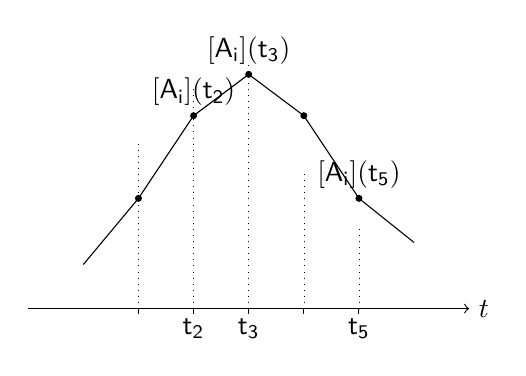
\begin{tikzpicture}[scale=0.7]
			
			\draw[->] (-1,0) -- (7,0) node[anchor=west] {$t$}; % t-axis
			
			% vertical lines
			\draw[line width=0.2pt,dotted] (1,0) -- (1,3);
			\draw[line width=0.2pt,dotted] (2,0) -- (2,4);
			\draw[line width=0.2pt,dotted] (3,0) -- (3,4.5);
			\draw[line width=0.2pt,dotted] (4,0) -- (4,2.5);
			\draw[line width=0.2pt,dotted] (5,0) -- (5,1.5);
			
			% draw ticks
			\foreach \x in {1,2,3,4,5}
			\draw (\x,0) -- (\x,-0.1);
			
			% averaged function
			\draw[line width=0.4pt] (0,0.8) -- (1,2);
			\draw[line width=0.4pt] (1,2) -- (2,3.5);
			\draw[line width=0.4pt] (2,3.5) -- (3,4.25);
			\draw[line width=0.4pt] (3,4.25) -- (4,3.5);
			\draw[line width=0.4pt] (4,3.5) -- (5,2);
			\draw[line width=0.4pt] (5,2) -- (6,1.2);
			
			\filldraw [black] (1,2) circle (1.5pt);
			\filldraw [black] (2,3.5) node[anchor=south] {$\mathsf{[A_i](t_2)}$} circle (1.5pt);
			\filldraw [black] (3,4.25) node[anchor=south] {$\mathsf{[A_i](t_3)}$} circle (1.5pt);
			\filldraw [black] (4,3.5) circle (1.5pt);
			\filldraw [black] (5,2) node[anchor=south] {$\mathsf{[A_i](t_5)}$} circle circle (1.5pt);]
			
			% time marks
			\filldraw [black] (2,0) node[anchor=north] {$\mathsf{t_2}$} circle (0.1pt);
			\filldraw [black] (3,0) node[anchor=north] {$\mathsf{t_3}$} circle (0.1pt);
		    \filldraw [black] (5,0) node[anchor=north] {$\mathsf{t_5}$} circle (0.1pt);
			
		\end{tikzpicture}
	\caption{Time-dependent behaviour of the chemical system: the molar concentrations of species $\mathsf{A_i}$ measured at consecutive time points.}
	\end{figure}
\ecol
%
\end{frame}

\begin{frame}{Quiz, Production/consumption rate}
	
	\begin{itemize}
		\item Consider the reaction 
		%
		$$\mathsf{a\, A + b\, B \rightleftharpoons c \, C + d \, D}.$$
		%
		\item Knowing that $r = \tfrac{1}{\nu_i}  \, \tfrac{d [ \mathsf{A_i}]}{dt} = \tfrac{1}{\nu_i} \, r(\mathsf{A_i}),$ where $\nu_i > 0$ for products and $\nu_i < 0$ for reactants. 
		%
		\pause
		\alert{\bf Quiz} (multiple choice): which statements about reaction/production rates are correct?
		%
		\vskip 5pt
		\begin{center}
    	\href{http://etc.ch/wsKw}{\textcolor{indigo(dye)}{\tt http://etc.ch/wsKw}} \quad
			or 
		    \quad	\includegraphics[height=0.12\columnwidth]{figures/chemical-kinetics/polls.png}
		\end{center}
		\hiddenpause 
		\vskip 10pt
		\item \alert{\bf Answer}: the correct relations on the reaction/production rates are
		%
		\begin{alignat*}{2}
		- \tfrac{1}{a} \, r(\mathsf{A}) & = \tfrac{1}{d}\,  r(\mathsf{D}) \quad \Rightarrow \quad r(\mathsf{A}) = - \tfrac{a}{d} \,  r(\mathsf{D}), \\[-3pt]
		- \tfrac{1}{b} \, r(\mathsf{B}) &  = \tfrac{1}{d} \,  r(\mathsf{D}), \\[-3pt]
		\tfrac{1}{c} \,  r(\mathsf{C})  & = \tfrac{1}{d} \,  r(\mathsf{D}) \quad \Rightarrow \quad r(\mathsf{C}) = \tfrac{c}{d} \,  r(\mathsf{D}).
		\end{alignat*}	
	\end{itemize}
\end{frame}
%
% --------------------------------------------------------------------------------------------------------------------%
% Reaction rate via concantrations of reactants
% --------------------------------------------------------------------------------------------------------------------%
%
\begin{frame}[shrink]{Reaction rate via concentrations of reactants}
%
\begin{itemize}
\item \alert{\bf Reaction rate for general equation}
%
\[0 \rightleftharpoons \sum_{i=1}^{N} \nu_i \, \mathsf{A_i},\]
%
can be defined {\bf proportional to the concentrations of the reactants raised to a power}:
%
\[r := k \prod_{i=1}^{N} [\mathsf{A_i}]^{\alpha_i},\]
%
where
%
\begin{itemize}
	\item $k > 0$ is the {\bf rate coefficient}, 
	\item $[\mathsf{A_i}]$ is a molar concentrations ($\mathsf{\tfrac{mol}{m^3}}$), 
	\item $\alpha_i > 0$ is the {\bf order of reaction with respect to species $\mathsf{A_i}$}, %such that $\alpha := \sum_{i}^{N} \alpha_i$ is the overall order of reaction, 
	and 
	\item $N$ is the number of species.
\end{itemize}
%
\end{itemize}
%
\end{frame}
%
\begin{frame}{Quiz, Reaction rate via concentration of reactants}
	
	\begin{itemize}
		\item Consider the elementary reaction 
		%
		$$\mathsf{a\, A + b\, B \rightleftharpoons c \, C + d \, D}.$$
		%
		\item 
		\alert{\bf Quiz}: what is the reaction rate of this reaction?
		%
		\vskip 5pt
		\begin{center}
    	\href{http://etc.ch/wsKw}{\textcolor{indigo(dye)}{\tt http://etc.ch/wsKw}} \quad
			or 
		    \quad	\includegraphics[height=0.12\columnwidth]{figures/chemical-kinetics/polls.png}
		\end{center}
		%
		\hiddenpause 
		\vskip 10pt
 		\item \alert{\bf Answer}: the correct reaction rate is 
 		$\mathsf{r = k {[A]}^a {[B]}^b}$.
	\end{itemize}
\end{frame}
% --------------------------------------------------------------------------------------------------------------------%
% Order of reaction vs. stoichiometry
% --------------------------------------------------------------------------------------------------------------------%
%
\begin{frame}{Order of reaction vs. stoichiometry}
	%
	\small
	\begin{itemize}
	\item The sum of the powers is \alert{\bf the overall order of the reaction}, i.e., 
	%
	\[\mathsf{\alpha = \sum_{i=1}^{N} \alpha_i}.\]
	%
	\pause
	\item For the overall reaction equation, \alert{\bf the order does not necessarily reflect the stoichiometry}, i.e., 
	%
	$\alpha_i \neq \nu_i$,
	%
	because of the {\bf intermediate steps} hidden in the overall reaction.\\[5pt]
	%
	{\bf Example}: in the reaction $\mathsf{CO + Cl_2 \xrightleftharpoons[]{r} COCl_2}$, the reaction rate $r = \mathsf{[CO]^2 \cdot [Cl_2]^{3/2}}$.
	%
%	\begin{itemize}
%		\item for $\mathsf{2\,NO + O_2 \xrightleftharpoons[]{k} 2\,NO_2}$: $k = \mathsf{[NO]^2 \cdot [O_2]}$;
%	    \item for $\mathsf{CO + Cl_2 \xrightleftharpoons[]{k} COCl_2}$: $k = \mathsf{[CO]^2 \cdot [Cl_2]^{3/2}}$.
%    \end{itemize}
	%
	\pause
	\vskip -5pt
	\pause
	\item For elementary reactions, {\bf the reaction orders and the absolute value of the stoichiometric
coefficients} of the reactants are \alert{\bf commonly the same}. \\[5pt]
%
    {\bf Example}:
	\begin{itemize}
	\item for unimolecular decomposition $\mathsf{A \xrightleftharpoons[]{r} B}$: $r = \mathsf{[A]}$
	%
	\item for bimolecular reaction \\[5pt]
 	$\bullet$ $\mathsf{A + B \xrightleftharpoons[]{r} C}$: $r = \mathsf{[A] \cdot [B]}$, or \\
	$\bullet$ $\mathsf{A + A \xrightleftharpoons[]{r} C}$: $r = \mathsf{[A]^2}$.
	\end{itemize}
\end{itemize}
	%
\end{frame}
%
\begin{frame}{Quiz, Order of reaction}
	
	\begin{itemize}
		\item Consider the reaction 
		%
		$$\mathsf{
		C_{6}H_{5}N_{2}Cl(aq) + H_{2}O (l) 
        \rightleftharpoons
        C_{6}H_{5}OH(aq) + N_{2}(g) + HCl(aq)}.$$
		%
		\item 
		\alert{\bf Quiz}: given that $\mathsf{r = k [C_{6}H_{5}N_{2}Cl(aq)]^1 [H_{2}O(l)]^0}$, what is the overall order of this reaction?
		%
		\vskip 5pt
		\begin{center}
    	\href{http://etc.ch/wsKw}{\textcolor{indigo(dye)}{\tt http://etc.ch/wsKw}} \quad
			or 
		    \quad	\includegraphics[height=0.12\columnwidth]{figures/chemical-kinetics/polls.png}
		\end{center}
		%
		\hiddenpause 
		\vskip 10pt
 		\item \alert{\bf Answer}: the overall order is 1.
	\end{itemize}
\end{frame}
% --------------------------------------------------------------------------------------------------------------------%
% Stoichometry in intermediate reactions
% --------------------------------------------------------------------------------------------------------------------%
%
\begin{frame}{Stoichiometry in intermediate reactions}
	%
	\small
	\begin{itemize}
		\item 
	The overall \alert{\bf reaction of hydrogen combustion} $\mathsf{2 \, H_2 + O_2 \rightleftharpoons 2\, H_2O}$ should contain the following intermediate steps (among total 30-40 steps):
	{\small
		\lcol
		\begin{alignat*}{2}
			R_1:  & \quad \mathsf{H_2 + O_2 \xrightleftharpoons[]{k_1} H + HO_2} \\
			R_2: & \quad \mathsf{O_2 + H \xrightleftharpoons[]{k_2} OH + O} \\
			R_3: & \quad \mathsf{H_2 + OH \xrightleftharpoons[]{k_3} H + H_2O} \\
		\end{alignat*}
	  \rcol
	  \vskip -30pt
	  \begin{alignat*}{2}
	  	R_4: & \quad \mathsf{H_2 + O \xrightleftharpoons[]{k_4} H + OH} \\
	  	R_5: & \quad \mathsf{O_2 + H + M \xrightleftharpoons[]{k_5} HO_2 + M} \\
	  	R_6: & \quad \mathsf{HO_2 + OH \xrightleftharpoons[]{k_6} H_2O + OH}.
	  \end{alignat*}
	  \ecol
	}
	%where $M$ is any species present in the mixture.
	%
	\pause
	\item Each {\bf elementary reaction step $j$} can be characterized by the stoichiometric equation
	%
	\[
	\sum_{i} \nu^R_{ji}	\mathsf{A_i} \xrightleftharpoons[]{k_j} \sum_{i} \nu^P_{ji} \mathsf{A_i}
	\]
	%
	\vskip -10pt
	\pause
	\item The \alert{\bf stoichiometric coefficient belonging to species $\mathsf{A_i}$ in a reaction step $j$} can be calculated by
	%
	\[
	\nu_{ji} = \nu^P_{ji} - \nu^R_{ji}.
	\]
\end{itemize}
	%
\end{frame}
%
% --------------------------------------------------------------------------------------------------------------------%
% Differential \& integral forms for the reaction rate, Half-time
% --------------------------------------------------------------------------------------------------------------------%
%
\begin{frame}[<+->]{Differential \& integral forms for the reaction rate, Half-time}
%
\footnotesize
\begin{itemize}
	\item To establish the relationship between the {\bf rate of change of the concentration of a reactant/product}  and  {\bf reaction rate} over time, i.e., 
	$$r := \tfrac{1}{\nu_i}  \, \tfrac{d [ \mathsf{A_i}]}{dt} \quad \mbox{and} \quad 
		r := k \prod_{i=1}^{N} [\mathsf{A_i}]^{\alpha_i},$$
	the {\bf differential equation} is used.
	\item For simple cases, it may be analytically integrated (see Table \ref{tab:differential-integral-forms}) to obtain \alert{\bf the integral form}.
	\item \alert{\bf The half-life of the reaction} is the time required for the reagent concentration be reduced to half of its initial
value.
\end{itemize}
\begin{table}
\footnotesize
	\begin{tabular*}{1\textwidth}{@{\extracolsep{\fill}}lcccc}
		\toprule 
		Reaction & Order & Differential Form & Integrated form & Half-time \\[5pt]
		\midrule 
		A $\rightarrow$ B & 0 & $-\tfrac{d \mathsf{[A]}}{dt} = k_0$ & $\mathsf{[A]} = \mathsf{[A]_0} - k_0\,t$ & 
		$t_{1/2} = \tfrac{\mathsf{[A]_0}}{2\,k_0}$ \\[5pt]
		A $\rightarrow$ B + C & 1 & $-\tfrac{d \mathsf{[A]}}{dt} = k_1\, \mathsf{[A]}$ & $\ln \mathsf{[A]} = \ln \mathsf{[A]_0} - k_1\,t$ & $t_{1/2} = \tfrac{\ln 2}{k_1}$ \\[5pt]
		A + B  $\rightarrow$ C & 2 & $-\tfrac{d \mathsf{[A]}}{dt} = k_2\, \mathsf{[A]}\, \mathsf{[B]}$ & 
		$k_2\,t = \tfrac{1}{\mathsf{[B]_0} + \mathsf{[A]_0}} \ln \tfrac{\mathsf{[B]_0} \mathsf{[A]}}{\mathsf{[B]} \mathsf{[A]_0}}$ & $t_{1/2} = \tfrac{1}{k_2 \, \mathsf{[A]_0}}$ (B = A) \\[5pt]
		\bottomrule
	\end{tabular*}
	%
	\caption{\label{tab:differential-integral-forms} \footnotesize Differential and integral forms for the reaction rate as well as half-time, where $\mathsf{[A]_0}$ and $\mathsf{[B]_0}$ correspond to the initial concentrations of A and B, respectively.}
\end{table}
%
\end{frame}
%
% --------------------------------------------------------------------------------------------------------------------%
% Example, Differential \& integral forms for the reaction rate, Half-time
% --------------------------------------------------------------------------------------------------------------------%
%
\begin{frame}{Quiz, Differential \& integral forms for the reaction rate, Half-time}
	%
	\begin{itemize}
		\item \alert{\bf Quiz}: Given a first-order reactant and rate constant  $k_1$ = 1.5e-4 1/min, what is the the half-life of the reactant if the time is defined by  $t_{1/2} = \tfrac{\ln 2}{k_1}$?
		%
		\begin{center}
			\href{http://etc.ch/wsKw}{\textcolor{indigo(dye)}{\tt http://etc.ch/wsKw}} 
			\quad or \quad  
			\includegraphics[height=0.2\columnwidth]{figures/chemical-kinetics/polls.png}
		\end{center}
 		\hiddenpause 
 		\vskip 10pt
 		\item {\bf Answer}: ln(2) / 1.5e-4 min = 
 		ln2 / 0.0000025 s $\approx$ 27.73e4 s
	\end{itemize}
	%
\end{frame}
%
\begin{frame}{Quiz, Reaction rate for the different order reactions}
	%
	\begin{itemize}
		\item \alert{\bf Quiz} (multi-choice): Knowing formulation of the reactions rate for different order reactions
		
		\begin{table}
\footnotesize
	\begin{tabular*}{1\textwidth}{@{\extracolsep{\fill}}lcccc}
		\toprule 
		Reaction & Order & Differential Form & Integrated form & Half-time \\[5pt]
		\midrule 
		A $\rightarrow$ B & 0 & $-\tfrac{d \mathsf{[A]}}{dt} = k_0$ & $\mathsf{[A]} = \mathsf{[A]_0} - k_0\,t$ & 
		$t_{1/2} = \tfrac{\mathsf{[A]_0}}{2\,k_0}$ \\[5pt]
		A $\rightarrow$ B + C & 1 & $-\tfrac{d \mathsf{[A]}}{dt} = k_1\, \mathsf{[A]}$ & $\ln \mathsf{[A]} = \ln \mathsf{[A]_0} - k_1\,t$ & $t_{1/2} = \tfrac{\ln 2}{k_1}$ \\[5pt]
		A + B  $\rightarrow$ C & 2 & $-\tfrac{d \mathsf{[A]}}{dt} = k_2\, \mathsf{[A]}\, \mathsf{[B]}$ & 
		$k_2\,t = \tfrac{1}{\mathsf{[B]_0} + \mathsf{[A]_0}} \ln \tfrac{\mathsf{[B]_0} \mathsf{[A]}}{\mathsf{[B]} \mathsf{[A]_0}}$ & $t_{1/2} = \tfrac{1}{k_2 \, \mathsf{[A]_0}}$ (B = A) \\[5pt]
		\bottomrule
	\end{tabular*}
	%
\end{table}
		\vskip 10pt
		%
		Which statements below are correct?
		%
		\begin{center}
			\href{http://etc.ch/wsKw}{\textcolor{indigo(dye)}{\tt http://etc.ch/wsKw}} 
			\quad or \quad  
			\includegraphics[height=0.1\columnwidth]{figures/chemical-kinetics/polls.png}
		\end{center}
		\hiddenpause 
		\vskip 10pt
		\item {\bf Answer}: Normally, the greater the concentration of reactants, the faster the reaction rate will occur. But this is not true of zero order reactions! 
	\end{itemize}
	%
\end{frame}
\begin{frame}
\centering
\includegraphics[height=0.6\textwidth]{figures/chemical-kinetics/maren-brener-slide.png}

\end{frame}
% --------------------------------------------------------------------------------------------------------------------%
% Mass action kinetics and corresponding kinetic system of ODEs
% --------------------------------------------------------------------------------------------------------------------%
%
\begin{frame}{Mass action kinetics and corresponding kinetic system of ODEs}
	%
	\footnotesize
	\begin{itemize}
		\item \alert{\bf The law of mass action kinetics} for elementary reactions can be formulated as
		%
		\[r_j := k_j \, \prod_{i=1}^{\mathsf{N}} \mathsf{[A_i]}^{\nu_{ji}}, \quad j = 1, \ldots, \mathsf{M}, \]
		\vskip -10pt
		%
		%
		where 
		\begin{itemize}
			\item $r_j $ is the kinetic rate of $j$th reaction step and $k_j$ is the $j$th rate coefficient, 
			\item $\mathsf{N}$ and $\mathsf{M}$ are the number of species and  the number of reactions, respectively, 
			\item $\nu_{ji}$ is the stoichiometric coefficient of the $i$th species, and 
			\item  $\mathsf{A_i}$ is the formula of the $i$th species, and $[\mathsf{A_i}]$ is its corresponding concentration.
		\end{itemize} 
	%
	\pause
	\item \alert{\bf Kinetic system of ordinary differential equations ODEs} defines the relationship between 
	{\bf production rates of the species} $\tfrac{d \mathsf{[A_i]}}{dt}$ and {\bf reaction rates} $r_j$:
	%
	\[
	\tfrac{d \mathsf{[A_i]}}{dt} = \sum_{j=1}^{\mathsf{M}} \nu_{ji} r_j, \quad i = 1, \ldots, \mathsf{N}.
	\]
	\vskip -5pt
	\pause
	\item The {\bf kinetic system of ODEs} and {\bf its initial values} together provide the following
	\alert{\bf initial value problem}
	%
	\[
	\tfrac{d \mathsf{[A_i]}}{dt} = \sum_{j=1}^{\mathsf{M}} \nu_{ji} r_j, 
	\quad [A_i](0) = [A_i]_0,
	\quad i = 1, \ldots, \mathsf{N}.
	\]
	\end{itemize}
	%
\end{frame}
%
% --------------------------------------------------------------------------------------------------------------------%
% Example: kinetics law of mass action for hydrogen combustion
% --------------------------------------------------------------------------------------------------------------------%
%
\begin{frame}{Example, Kinetics law of mass action for hydrogen combustion}
		\begin{itemize}
		\item The overall reaction $\mathsf{2 \, H_2 + O_2 \rightleftharpoons 2\, H_2O}$ can be 
		decomposed into the following $M=6$ elementary steps with corresponding 
		the stoichiometry matrix $\nu \in \mathbb{R}^{6 \times 8}$, $\nu = \{\nu_{i, j}\}_{i = 1, ...,6; j = 1, ..., 8}$
			\lcol
			{\scriptsize
			\begin{alignat*}{4}
				R_1:  & \quad \mathsf{H_2 + O_2 \xrightleftharpoons[]{k_1} H + HO_2}    & \quad & r_1 = k_1  \mathsf{[H_2][O_2] } \\[-5pt]
				R_2: & \quad \mathsf{O_2 + H \xrightleftharpoons[]{k_2} OH + O}           && r_2 = k_2  \mathsf{[O_2][H] } \\[-5pt]
				R_3: & \quad \mathsf{H_2 + OH \xrightleftharpoons[]{k_3} H + H_2O}     && r_3 = k_3  \mathsf{[H_2][OH] } \\[-5pt]
				R_4: & \quad \mathsf{H_2 + O \xrightleftharpoons[]{k_4} H + OH}           && r_4 = k_4  \mathsf{[H_2][O] } \\[-5pt]
				R_5: & \quad \mathsf{O_2 + H + M \xrightleftharpoons[]{k_5} HO_2 + M} && r_5 = k_5  \mathsf{[O_2][H][M] } \\[-5pt]
				R_6: & \quad \mathsf{HO_2 + OH \xrightleftharpoons[]{k_6} H_2O + O_2} && r_6 = k_6  \mathsf{[HO_2][OH] }
			\end{alignat*}
			}
			\rcol
			{\small
				\vskip -30pt
			\only<1	>{
			\vskip 15pt
			\[
			\nu = 
			\kbordermatrix{
				& \mathsf{H} & \mathsf{H_2} & \mathsf{HO_2} & \mathsf{H_2O} & \mathsf{O} & \mathsf{O_2} & \mathsf{OH} & \mathsf{M} \\
				R_1 &   1 & -1 & 1 & 0 & 0 & \alert{*} & 0 & 0\\[10pt]
				R_2 & -1 &  0 & 0 & 0 & 1 & \alert{*} & 1 & 0\\[10pt]
				R_3 &   1 & -1 & 0 & 1 & 0 & \alert{*} & -1 & 0\\[5pt]
				R_4 &  1 & -1 & 0 & 0 & -1 & \alert{*} & 1 & 0\\[5pt]
				R_5 & -1 &  0 & 1 & 0 & 0 & \alert{*} & 0 & 0\\[5pt]
				R_6 &  0 &  0 & -1 & 1 & 0 & \alert{*} & -1 & 0\\[5pt]
			}
			\]
			}
			\only<2>{
			\vskip 15pt
			\[
			\nu = 
			\kbordermatrix{
				& \mathsf{H} & \mathsf{H_2} & \mathsf{HO_2} & \mathsf{H_2O} & \mathsf{O} & \mathsf{O_2} & \mathsf{OH} & \mathsf{M} \\
				R_1 &   1 & -1 & 1 & 0 & 0 & \alert{-1} & 0 & 0\\[10pt]
				R_2 & -1 &  0 & 0 & 0 & 1 & \alert{-1} & 1 & 0\\[10pt]
				R_3 &   1 & -1 & 0 & 1 & 0 & \alert{0} & -1 & 0\\[5pt]
				R_4 &  1 & -1 & 0 & 0 & -1 & \alert{0} & 1 & 0\\[5pt]
				R_5 & -1 &  0 & 1 & 0 & 0 & \alert{-1} & 0 & 0\\[5pt]
				R_6 &  0 &  0 & -1 & 1 & 0 & \alert{1} & -1 & 0\\[5pt]
			}
			\]
			}
			}
			\ecol
	%
	\vskip 5pt 
	\item \alert{\bf Quiz}: What are the coefficients in the column with the O$_2$? \\[5pt]
	\begin{center}
		\href{http://etc.ch/wsKw}{\textcolor{indigo(dye)}{\tt http://etc.ch/wsKw}} \quad or \quad
		\includegraphics[height=0.09\columnwidth]{figures/chemical-kinetics/polls.png}
	\end{center}
%	\item The production rates can be formulated as follows: 
%	{\footnotesize
%	\begin{alignat*}{2}
%		\tfrac{d\mathsf{H}}{dt} = & 1 \, r_1 - 1 \, r_2 + 1 \, r_3 + 1 \, r_4 -  1 \, r_5 + 0 \, r_6\\
%								  = &  k_1  \mathsf{[H_2][O_2] } - k_2  \mathsf{[O_2][H] } + k_3  \mathsf{[H_2][OH]}  + k_4  \mathsf{[H_2][O] } -  k_5  \mathsf{[H][O_2][M]} + 0 \, k_6  \mathsf{[HO_2][OH] }\\
%		\tfrac{d\mathsf{H_2O}}{dt} = & 1 \, r_3 + 1 \, r_6 
%		= k_3  \mathsf{[H_2][OH]} + k_6  \mathsf{[HO_2][OH] }\\
%	\end{alignat*}
%	}
	%
	\end{itemize}
\end{frame}
%
\begin{frame}{Example, Kinetics law of mass action for hydrogen combustion}
	\lcol
	{\scriptsize
		\begin{alignat*}{4}
			R_1:  & \quad \mathsf{H_2 + O_2 \xrightleftharpoons[]{k_1} H + HO_2}    & \quad & r_1 = k_1  \mathsf{[H_2][O_2] } \\[-5pt]
			R_2: & \quad \mathsf{O_2 + H \xrightleftharpoons[]{k_2} OH + O}           && r_2 = k_2  \mathsf{[O_2][H] } \\[-5pt]
			R_3: & \quad \mathsf{H_2 + OH \xrightleftharpoons[]{k_3} H + H_2O}     && r_3 = k_3  \mathsf{[H_2][OH] } \\[-5pt]
			R_4: & \quad \mathsf{H_2 + O \xrightleftharpoons[]{k_4} H + OH}           && r_4 = k_4  \mathsf{[H_2][O] } \\[-5pt]
			R_5: & \quad \mathsf{O_2 + H + M \xrightleftharpoons[]{k_5} HO_2 + M} && r_5 = k_5  \mathsf{[O_2][H][M] } \\[-5pt]
			R_6: & \quad \mathsf{HO_2 + OH \xrightleftharpoons[]{k_6} H_2O + O_2} && r_6 = k_6  \mathsf{[HO_2][OH] }
		\end{alignat*}
	}
	\rcol
	{\small
		\vskip -30pt
		\[
		\nu = 
		\kbordermatrix{
			& \mathsf{H} & \mathsf{H_2} & \mathsf{HO_2} & \mathsf{H_2O} & \mathsf{O} & \mathsf{O_2} & \mathsf{OH} & \mathsf{M} \\
			R_1 &   1 & -1 & 1 & 0 & 0 & -1 & 0 & 0\\[10pt]
			R_2 & -1 &  0 & 0 & 0 & 1 & -1 & 1 & 0\\[10pt]
			R_3 &   1 & -1 & 0 & 1 & 0 & 0 & -1 & 0\\[5pt]
			R_4 &  1 & -1 & 0 & 0 & -1 & 0 & 1 & 0\\[5pt]
			R_5 & -1 &  0 & 1 & 0 & 0 & -1 & 0 & 0\\[5pt]
			R_6 &  0 &  0 & -1 & 1 & 0 & 1 & -1 & 0\\[5pt]
		}
		\]
	}
	\ecol
	\vskip 5pt
	\begin{itemize}
		\item The production rates can be formulated as follows: 
		{\footnotesize
			\begin{alignat*}{2}
				\tfrac{d\mathsf{H}}{dt} = & 1 \, r_1 - 1 \, r_2 + 1 \, r_3 + 1 \, r_4 -  1 \, r_5 + 0 \, r_6\\
				= &  k_1  \mathsf{[H_2][O_2] } - k_2  \mathsf{[O_2][H] } + k_3  \mathsf{[H_2][OH]}  + k_4  \mathsf{[H_2][O] } -  k_5  \mathsf{[H][O_2][M]} + 0 \, k_6  \mathsf{[HO_2][OH] }\\[-15pt]
				%\tfrac{d\mathsf{H_2O}}{dt} = & 1 \, r_3 + 1 \, r_6 
				%= k_3  \mathsf{[H_2][OH]} + k_6  \mathsf{[HO_2][OH] }\\
			\end{alignat*}
		}
		%\vskip -35pt
		\item \alert{\bf Quiz}: What is the right-hand side for the $\tfrac{d\mathsf{HO_2}}{dt}$?
		%\begin{right}
			\href{http://etc.ch/wsKw}{\textcolor{indigo(dye)}{\tt http://etc.ch/wsKw}} \quad or \quad
			\includegraphics[height=0.08\columnwidth]{figures/chemical-kinetics/polls.png}
		%\end{right}
		%
		\vskip 10pt
		\hiddenpause
		\item {\bf Answer}:  $\tfrac{d\mathsf{HO_2}}{dt} = 1 \, r_1  + 1 \, r_5 -1  \, r_6 = k_1  \mathsf{[H_2][O_2] } + k_5  \mathsf{[H][O_2][M]}  - \, k_6  \mathsf{[HO_2][OH] }.$
	\end{itemize}
\end{frame}
%
% --------------------------------------------------------------------------------------------------------------------%
% Exercises: mass action and production rates
% --------------------------------------------------------------------------------------------------------------------%
%
%\begin{frame}{Exercises}
%	\begin{itemize}
%		\item 
%		Consider the overall reaction of hydrogen combustion $\mathsf{2 \, H_2 + O_2 \rightleftharpoons 2\, H_2O}$ that is decomposed into the following $M$ ementary steps $M = 6$:
%		\begin{alignat*}{4}
%			R_1:  & \quad \mathsf{H_2 + O_2 \xrightleftharpoons[]{k_1} H + HO_2    && r_1 = k_1  \mathsf{[H_2][O_2] } \\
%			R_2: & \quad \mathsf{O_2 + H \xrightleftharpoons[]{k_2} OH + O           && r_1 = k_1  \mathsf{[H_2][O_2] } \\
%			R_3: & \quad \mathsf{H_2 + OH \xrightleftharpoons[]{k_3} H + H_2O     && r_1 = k_1  \mathsf{[H_2][O_2] } \\
%			R_4: & \quad \mathsf{H_2 + O \xrightleftharpoons[]{k_4} H + OH           && r_1 = k_1  \mathsf{[H_2][O_2] } \\
%			R_5: & \quad \mathsf{O_2 + H + M \xrightleftharpoons[]{k_5} HO_2 + M && r_1 = k_1  \mathsf{[H_2][O_2] } \\
%			R_6: & \quad \mathsf{HO_2 + OH \xrightleftharpoons[]{k_6} H_2O + OH && r_1 = k_1  \mathsf{[H_2][O_2] }
%		\end{alignat*}
%		%
%		\item {\bf Exercises}: 
%		\begin{itemize}
%			\item Using the kinetics law of mass action, formulate the rates $r_j$, where $j = 1, \ldots, M$.
%			\item Assume that $N$ species (where $N = 8$) are ordered as H, $\mathsf{H_2}, \mathsf{HO_2}, \mathsf{H_2O},  \mathsf{O}, \mathsf{O_2}, \mathsf{OH}$ and M.  
%			\item Using stoichometry matrix $\nu \in \mathbb{R}^{6 \times 8}$, 
%			formulate production rates of the species, i.e., $\tfrac{\mathsf{H}}{dt}$, ..., $\tfrac{\mathsf{M}}{dt}$.
%		\end{itemize}
%	\end{itemize}
%\end{frame}
%
% --------------------------------------------------------------------------------------------------------------------%
% Temperature dependence of rate coefficients, Arrhenius equation
% --------------------------------------------------------------------------------------------------------------------%
%
\subsection{Reaction rate and its dependence on temperature and pressure}
\begin{frame}{Temperature dependence of rate coefficients, Arrhenius equation}
	\begin{itemize}
		\item {\bf The temperature dependence of rate coefficient} $k$ is	described by the \alert{\bf (classic) Arrhenius equation}:
		%
		\[
		k := A\, e^{-\tfrac{E_a}{R\, T}},\]
		%
		where 
		\begin{itemize}
			\item $A$ is the pre-exponential factor or A-factor,
			\item $E_a$ is the activation energy ($\tfrac{\rm J}{\rm mol}$), 
			\item $R = 8.314$ is the gas constant ($\tfrac{\rm J}{\rm mol \, K}$), and 
			\item $T$ is the temperature (K).
		\end{itemize}
		%
		\pause
		\item $E_a$ is is the {\bf minimum energy} that the reactant molecules must possess before the reaction can occur (bigger $E_a$ is $\Rightarrow$ smaller is the reaction rate $\Rightarrow$ slower the reaction will proceed).
		\pause
		\item $E_a$ is {\bf determined experimentally} by performing the reaction at several temperatures. 
		%\pause
		%\item The dimension of quantity $E/R$ is temperature and it is called the \alert{\bf activation temperature}. 
	\end{itemize}
\end{frame}
%
% --------------------------------------------------------------------------------------------------------------------%
% Temperature dependence of rate coefficients, Arrhenius plot
% --------------------------------------------------------------------------------------------------------------------%
%
% Important thing to mention after we have introduced the reaction rate is actually how it depends on the temperature. 
%
\begin{frame}{Temperature dependence of rate coefficients, Arrhenius plot}
	\begin{itemize}
		\item After taking the {\bf natural logarithm of the Arrhenius equation}, one obtains
		%
		\[
		\underbrace{\ln k}_\text{$y$} := \ln A - \tfrac{E_a}{R} \, \underbrace{\tfrac{1}{T}}_\text{$x$},
		\]
		%
		\item Then, the  graph of $y = \ln A - \tfrac{E_a}{R} \, x$ is a \alert{\bf linear function}
		with slope $\tan \alpha = - \tfrac{E_a}{R}$ and intersect $ \ln A$:
		%
		  \begin{figure}
		  	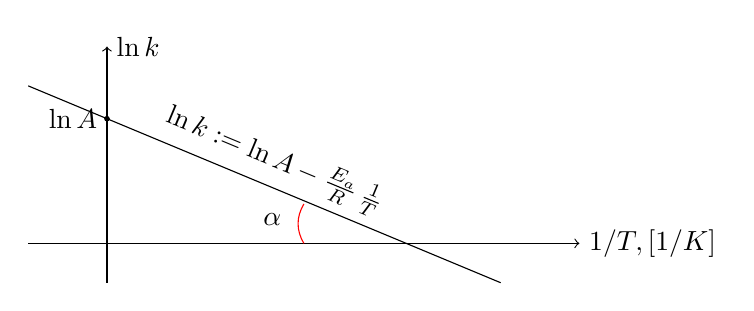
\begin{tikzpicture}
		  		
		  		% coordinate axis
		  		\draw[->] (-1,0) -- (6,0) node[anchor=west] {$1/T, [1/K]$};
		  		\draw[->] (0,-0.5) -- (0,2.5) node[anchor=west] {$\ln k$};
		  		
		  		% intersection with vertical axis
		  		\filldraw[black] (intersection cs: first line={(-1,2)--(5,-0.5)},
		  		                         second line={(0,-1) -- (0,4)}) node[anchor=east] {$\ln A$} circle (0.8pt);
		  		
		  		% linear function
		  		\draw (-1,2) to node  [sloped,above] {$\ln k := \ln A - \tfrac{E_a}{R} \, \tfrac{1}{T}$} (5,-0.5);
		  		
		  		%
		  		\draw[red] (2.5,0) to[bend left] (2.5, 0.5);
		  		\draw (2.1,0.3) node {$\alpha$};
		  	\end{tikzpicture}
	  	  \caption{Linear function $\ln k := \ln A - \tfrac{E_a}{R} \, \tfrac{1}{T}$.}
		  \end{figure}

	\end{itemize}
\end{frame}
%
% --------------------------------------------------------------------------------------------------------------------%
% Temperature dependence of rate coefficients, alternative forms of Arrhenius equation
% --------------------------------------------------------------------------------------------------------------------%
%
\begin{frame}{Alternative forms of Arrhenius equation}
	\begin{itemize}
		\item In {\bf high-temperature gas-phase kinetic systems} (e.g., combustion systems) the temperature dependence of the rate coefficient is described by the 
		\alert{\bf modified / extended Arrhenius equation}:
		%
		\[
		k := B\,\alert{T^n} e^{-\tfrac{C}{R\, T}},
		\]
		%
		where $B \neq A$ and $C \neq E_a$.
		%
%		\item If the temperature dependence of the rate coefficient is described by the modified Arrhenius equation, 
%		then the activation energy $E_a$ changes linearly  with temperature.
%		{\bf Exercises}: show that %, if $E_a(T)$ can be calculated 
%		%as the derivative of the temperature function with respect to $1/T$, i.e.,
%	    \[ E_a(T):=\frac{d \ln k}{d (1/T)} = n\,R\,T + C.\]%, where $\ln k := \ln B + n\, \ln T - \tfrac{C}{R} \, \tfrac{1}{T}$.
		%
		\item For some {\bf gas-phase kinetic elementary reactions}, the temperature dependence of 
		the rate coefficient is described by a 	\alert{\bf truncated form of the extended Arrhenius equation}
		%
		\[
		k= A\,T^n.
		\]
	\end{itemize}

\end{frame}
%
% --------------------------------------------------------------------------------------------------------------------%
% Rate coefficient, methan reaction example
% --------------------------------------------------------------------------------------------------------------------%
%
\begin{frame}{Example of methane reaction, Arrhenius plots comparison}
	\lcol
	\begin{itemize}
			\item Reaction of {\bf methane consumption in the troposphere} $\mathsf{CH_4+OH  \xrightleftharpoons[]{} CH_3+H_2O}$, 
			happens in a range between 220 K (-53 \textdegree C) and 320 K (+47 \textdegree C). 
		%where the rate coefficient can be described by $k := A\, e^{-\tfrac{E}{R\, T}}$.
	\end{itemize}
	\rcol
	\begin{itemize}
		\item In {\bf methane flames}, it is one of the main consuming reactions of the {\bf fuel molecules}, where 
		$T$ ranges between 300 K (27 \textdegree C) and 2,200 K (maximum temperature of a laminar
		premixed methane-air flame). %Then, $k := A\,T^n\, e^{-\tfrac{E}{R\, T}}$.
		%When representing the temperature dependence of the
		%rate coefficient within this wide temperature range in an Arrhenius plot, the
		%obtained function is clearly curved (see Fig. 2.2b).
	\end{itemize}
	\ecol
	\begin{figure}[!t]
		\centering
		\subfloat[Arrhenius plot]{\includegraphics[width=0.4\textwidth]{figures/chemical-kinetics/arrhenius-plot}} \qquad \qquad
 		\subfloat[Extended Arrhenius plot]{\includegraphics[width=0.38\textwidth]{figures/chemical-kinetics/extended-arrhenius-plot}}
	\end{figure}
\end{frame}
%
% --------------------------------------------------------------------------------------------------------------------%
% Pressure dependence of rate coefficients, Lindemann model
% --------------------------------------------------------------------------------------------------------------------%
%
\begin{frame}{Pressure dependence of rate coefficients, Lindemann model \, i}
	\begin{itemize}
		\item According to \alert{\bf Lindemann model}, a unimolecular decomposition is only possible if {\bf the energy in the molecule is 
		sufficient to break the bond}.
		\item Before decomposition, the energy must be added to A by means of collision with M (representation of the pressure) to obtain excited molecule A$^\star$:
		 \begin{alignat*}{2}
			\mbox{Activation} : & \quad \mathsf{A + M \xrightleftharpoons[]{k_1} A^\star + M} \\
			\mbox{Deactivation}: & \quad \mathsf{A^\star + M \xrightleftharpoons[]{k_2} A + M} \\
			\mbox{Unimolecular reaction}: & \quad \mathsf{A^\star \xrightleftharpoons[]{k_3} C}
		 \end{alignat*}
		\item The {\bf production rates} can be written as: 
		%
		 \begin{alignat*}{2}
			\tfrac{d\mathsf{[C]}}{dt}          & = k_3 \, \mathsf{[A^\star]} \\
			\tfrac{d\mathsf{[A^\star]}}{dt} & 
			= \sum_{i = 1, \ldots, 3} \nu_i r_i 
			=  r_1 - r_2 - r_3 
			= k_1 \, \mathsf{[A][M]} - k_2 \, \mathsf{[A^\star][M]} + k_3 \, \mathsf{[A^\star]}
		\end{alignat*}
	\end{itemize}
\end{frame}
%
% --------------------------------------------------------------------------------------------------------------------%
% Pressure dependence of rate coefficients, Lindemann model \, ii
% --------------------------------------------------------------------------------------------------------------------%
%
\begin{frame}{Pressure dependence of rate coefficients, Lindemann model \, ii}
	\begin{itemize}
		\item Assuming steady-state for $\mathsf{[A^\star]}$, meaning that $\tfrac{d[\mathsf{A^\star}]}{dt} = 0$, we obtain
		%
		\[
		\mathsf{[A^\star]} = \tfrac{k_1 \, \mathsf{[A]\, [M]}}{\alert<2>{k_2 \, [M]} + k_3} \qquad \mbox{and}  \qquad
		\tfrac{d\mathsf{[C]}}{dt} = \tfrac{k_1 \, k_3 \, \mathsf{[A]\, [M]}}{\alert<2>{k_2 \, [M]}  + k_3}, 
		\]
		where M represents applied pressure.\\[5pt]
	\end{itemize}
% 	\begin{itemize}
% 		%
% 		\item {\bf Under low pressure}, [M] is very small ($k_2\, \mathsf{M} \ll k_3$), then 
% 		%
% 		\[	
% 		\tfrac{d\mathsf{[C]}}{dt} = k_{\sf low} \, \mathsf{[A]\, [M]},
% 		\]
% 		%
% 		where $k_{\sf low}$ is the {\bf reaction rate coefficient at low pressure}.\\[5pt]
% 		%
% 		\pause
% 		\item {\bf For high pressure}, [M] is large  ($k_2\, \mathsf{M} \gg k_3$), then 
% 		%
% 		\[	
% 		\tfrac{d\mathsf{[C]}}{dt} = k_{\sf high} \, \mathsf{[A]},
% 		\]
% 		%
% 		where $k_{\sf high} $ is the {\bf reaction rate coefficient at high pressure}.
% 	\end{itemize}
    \vskip 20pt
	\lcol
	%\vskip 5pt
	{\bf For low pressure}: [M] is small ($k_2\, \mathsf{M} \ll k_3$), then 
	%
	\[	
	\tfrac{d\mathsf{[C]}}{dt} = k_{\sf low} \, \mathsf{[A]\, [M]},
	\]
	%
	where $k_{\sf low}$ is the {\bf reaction rate coefficient at low pressure}.
	\rcol
	{\bf For high pressure}: [M] is large  ($k_2\, \mathsf{M} \gg k_3$), then 
	%
	\[	
	\tfrac{d\mathsf{[C]}}{dt} = k_{\sf high} \, \mathsf{[A]},
	\]
	%
	where $k_{\sf high} $ is the {\bf reaction rate coefficient at high pressure}.
	\ecol
\end{frame}
%
% --------------------------------------------------------------------------------------------------------------------%
%% Reaction classification
%% --------------------------------------------------------------------------------------------------------------------%
%%
%\begin{frame}{Reaction classification}
%	\begin{itemize}
%		\item \alert{\bf Homogeneous} or \alert{\bf heterogeneous}:
%		\begin{itemize}
%			\item A {\bf homogeneous} reaction involves a single phase, e.g., 
%			%
%			\begin{alignat*}{2}
%			\mbox{Formation of ammonia}:  \mathsf{N_2(g) + 3\,H_2(g) } & \mathsf{\xrightleftharpoons[]{} 2\,NH_3(g)}\\
%			\mbox{Oxidation of sulfur dioxide}: \mathsf{2\,SO_2(g) + O_2(g) } & \mathsf{\xrightleftharpoons[]{} 2\,SO_3(g)} 
%			\end{alignat*}
%		    %
%			\item A {\bf heterogeneous} reaction involves more than one phase, e.g., 
%			\begin{alignat*}{2}
%			\mbox{Carbonatation} : \mathsf{Ca(OH)_2(s) + CO_2(g)} & \mathsf{\xrightleftharpoons[]{} CaCO_3(s) + H_2O(l)}
%	    	\end{alignat*}
%		\end{itemize}
% 	 	\item \alert{\bf Irreversible} or \alert{\bf reversible}:
%		\begin{itemize}
%			\item An {\bf irreversible} reaction is one that occurs in only one direction and continues in this direction until at least one of the reactants is depleted.
%			\item A {\bf reversible} reaction can occur in both directions (with forward and backward reaction reaction coeff. $k_f$ and $k_b$, respectively):
%			%
%			\[	
%			\mathsf{a\,A + b\,B} \xrightleftharpoons[k_f]{k_b} \mathsf{c\,C + d\,D} 
%			\quad 
%			\mbox{with equilibrium constant}
%			\quad
%			K_e := \tfrac{k_f}{k_b} = \tfrac{\mathsf{[C]^c\, [D]^d}}{\mathsf{[A]^a\,[B]^b}}.
%			\]
%			%
%		\end{itemize}
%	\end{itemize}
%\end{frame}
%
%
\begin{frame}[<+->]{Summary on reactions, their rates, rate coefficients, and orders}
	%
	\small
	\begin{itemize}
		\item The \alert{\bf overall reaction mechanism} is the result of {\bf all the elementary reactions mechanism}.
		%
		\item {\bf The reaction rate} and {\bf the reaction rate coefficient} are \alert{\bf determined by experiments}.
		%
% 		\item \alert{\bf The units of the reaction rate coefficients} $k$ depend on the relation 
% 		$[k] = \tfrac{1}{\mathsf{s \, [mol/m^3]}^{n-1}}$, where $n$ is the order of reaction. \\
		%{\bf Example}: for  the rate law $\tfrac{dw}{dt} = k \mathsf{[A][B]}$ of the second-order reaction, 
		%$[k] = \tfrac{\mathsf{m^3}}{\mathsf{s \, mol}}$. 
		%
		%
		\item {\bf The orders} are generally \alert{\bf not equal} to {\bf the stoichiometric coefficients} of the overall
		reaction equation.
		%
%		\item Unlike elementary reactions, the overall reaction rate {\bf may contain the concentration of
%		reactants, products, and catalysts}, but generally {\bf does not contain concentrations
%		of reactive intermediates}.
		%
		\item {\bf The order of reaction} is determined \alert{\bf experimentally} or by \alert{\bf means of mathematical models}.
		%
		\item The \alert{\bf most important reactions} are of: 
		\begin{itemize}
			\item zero order, 
			\item first order, and 
			\item second order.
		\end{itemize}
		%
		\item Third-order reactions {\bf are quite rare}, reactions of order greater than three are {\bf not known}.
		%	
		
	\end{itemize}
	%
\end{frame}
%
\subsection{Reaction mechanisms}
%
% --------------------------------------------------------------------------------------------------------------------%
% Reaction mechanism
% --------------------------------------------------------------------------------------------------------------------%
%
\begin{frame}{Reaction mechanisms}
	%
	\small
	\begin{itemize}
		\item The \alert{\bf kinetic mechanisms} can contain basically {\bf three types of reactions}:
		%
		\begin{itemize}
			\item in series (consecutive reactions), 
			\item in parallel (competitive reactions), and 
			\item independent.
		\end{itemize}
		%
		\pause
		\item \alert{\bf In series occurring reactions} (consecutive reactions), reactant forms an {\bf intermediate product}, which subsequently reacts to form another product:
		%
		\[\mathsf{A} \xrightleftharpoons[]{k_1} \mathsf{B} \xrightleftharpoons[]{k_2} \mathsf{C}. \]
		%
		%
		\pause
		\item \alert{\bf In parallel reactions} (competitive reactions), the reagent is consumed by two different reaction paths to form {\bf different products}:
		%
		\[\mathsf{A} \xrightleftharpoons[]{k_1} \mathsf{B} \quad \mbox{and}\quad \mathsf{A} \xrightleftharpoons[]{k_2} \mathsf{C}. \]
		%
		\pause
		\item Usually, kinetic mechanisms involve {\bf a combination of both reactions in series or parallel}.
	\end{itemize}
	%
\end{frame}
%
% --------------------------------------------------------------------------------------------------------------------%
% Example, Formation of butadiene C4H6 from ethanol
% --------------------------------------------------------------------------------------------------------------------%
%
\begin{frame}{Example, Formation of butadiene C$_4$H$_6$ from ethanol}
	%
	\begin{itemize}
		\item \alert{\bf Butadiene} $\mathsf{C_4H_6}$ is the organic compound, colorless gas that is easily condensed to a liquid.
		%
		\pause
		\item It is important industrially as a monomer in the \alert{\bf production of synthetic rubber}. 
		%
		\pause
		\item In South America, Eastern Europe, China, and India, butadiene is {\bf produced from ethanol}:		
		%
		%\item The kinetic mechanisms involve reactions in series or parallel:
		%
		%
	\end{itemize}
	\lcol
	\pause
	\begin{alignat*}{2}
		& \mathsf{C_2H_5OH \xrightleftharpoons[]{} C_2H_4 + H_2O,} \quad \mbox{(parallel)}\\
		& \mathsf{C_2H_5OH \xrightleftharpoons[]{} CH_3CHO + H_2,}  \quad \mbox{(parallel)}\\
		& \mathsf{C_2H_4 + CH3CHO \xrightleftharpoons[]{}  C_4H_6 + H_2O.}  \quad \mbox{(series)}
	\end{alignat*}
	\rcol
	\begin{figure}[!t]
		\includegraphics[scale=0.15]{figures/chemical-kinetics/butadiene.png}
		\caption{Organic compound of $\mathsf{(CH2=CH)_2}$.}
	\end{figure}
	\ecol
	%
\end{frame}
%
% --------------------------------------------------------------------------------------------------------------------%
% Chain reactions, Ignition of hydrogen
% --------------------------------------------------------------------------------------------------------------------%
%
\begin{frame}[<+->]{Chain reactions, Ignition of hydrogen example}
	\small
	%
	\begin{itemize}
		\item \alert{\bf Chain reactions} (type of the consecutive reactions) are defined by reactives intermediate reacting to produce another intermediates, 
		have complex kinetics, and occur quickly.
		%
		\item The intermediate species in a chain reaction is \alert{\bf a chain propagator}:
		%
		\begin{multline*}
			\mbox{reactant} \xrightarrow[]{\text{initiation}} \mbox{propagator 1} \xrightarrow[]{\text{chain branch i}} \ldots
			\xrightarrow[]{\text{chain branch i}} \mbox{propagator i} \xrightarrow[]{\text{termination}} \mbox{products} 
		\end{multline*}
		%
		\item They are the basis of \alert{\bf combustion processes}, rapid reactions of species with O$_2$ generating heat. 
		%
	\end{itemize}
	\begin{table}
		\begin{tabular*}{1\textwidth}{@{\extracolsep{\fill}}lll}
			\toprule 
			N & Reaction & Step \\[-5pt]
			\midrule 
			1 & $\mathsf{H_2 + O_2 \xrightleftharpoons[]{} 2\, OH^\star}$ &	initiation of the step \\[-3pt]
			2 & $\mathsf{OH^\star + H_2 \xrightleftharpoons[]{} H_2O + H^\star}$ &	propagation of the chain \\[-3pt]
			3 & $\mathsf{H^\star + O_2 \xrightleftharpoons[]{} OH^\star + O^\star}$ & branch of the chain \\[-3pt]
			4 & $\mathsf{O^\star + H_2 \xrightleftharpoons[]{} OH^\star + H^\star}$ & branch of the chain  \\[-3pt]
			5 & $\mathsf{H^\star \xrightleftharpoons[]{} 0.5 \, H_2}$ &	termination of the chain \\[-3pt]
			6 & $\mathsf{H^\star + O_2 + M \xrightleftharpoons[]{} HO_2^\star +M^\star }$ & propagation of the chain \\[-3pt]
			\bottomrule
		\end{tabular*}
		%
		\caption{Important reactions for the hydrogen ignition mechanism.}
	\end{table}
	%
\end{frame}
%
\subsection{Redox reaction}
%	
% --------------------------------------------------------------------------------------------------------------------%
% Redox reaction
% --------------------------------------------------------------------------------------------------------------------%
%
\begin{frame}{Redox reaction}
	\small
	\begin{itemize}
		\item \alert{\textbf{Redox (or reduction-oxidation) reaction}} is a type of chemical reaction that involves a transfer 
		of electrons between two species.
		\pause
		\item { \bf Examples}: 
		\begin{itemize}
				\item body uses redox reactions to convert food and oxygen to energy plus water and CO2;
				\item batteries in electronics rely on redox reactions;
				\item combustion reactions in the car engines, e.g., combustion of octane (hydrocarbon)
				%
				\[
				\mathsf{2 \, C_8\, H_{18} + 25\,O_2 \rightarrow 16\, CO_2(g) + 18\,H_2O}.
				\]			
		\end{itemize}
		%
		\pause
		\item The $\mathsf{H_2O}$ can be 
		%
		\begin{itemize}
			%\item ionized
			%%
			%\[
			%\mathsf{H_2O(l) = H^+ + OH^-,}
			%\]
			%
			\item (or oxygen in it) \alert{\bf oxidized}, losing electron, 
			%
			$\mathsf{H_2O(l) = O_2(aq) + 2\, e^{-} + 2\, H^+,}$ or 
			
			%
			\item (or hydrogen in it) \alert{\bf reduced}, accepting electron, 
			%
			%\[
			$
			\mathsf{H_2O(l) + e^{-} = \tfrac{1}{2} \, H_2(aq) + OH^-.}$
			%\]
			%
		\end{itemize}
		%
		\pause
		\item \alert{\bf Self-redox} is the reaction, where the same element undergoes oxidation and reduction simultaneously,  
		\[
		\mathsf{2\, NaOH + Cl_2 \rightarrow NaCl + NaClO + H_2O,}
		\]
		%
		where Cl$^0$ with oxidation number 0, becomes Cl$^{-1}$  in NaCl and Cl$^{+1}$  in NaClO. 
	\end{itemize}
\end{frame}
%
% --------------------------------------------------------------------------------------------------------------------%
% Oxidation number, Oxidizers and reducers 
% --------------------------------------------------------------------------------------------------------------------%
%
\begin{frame}{Oxidation number, Oxidizers and reducers }
	\small
	\begin{itemize}
		\item \alert{\textbf{Oxidation number}} (NOX) of a chemical element is  the number of charges that an atom would 
		possess if the electrons were not shared but located entirely on a single atom.
	\end{itemize}
	%
	\pause 
	\vskip -25pt
	\begin{columns}
		\begin{column}{0.6\textwidth}
			\begin{itemize}
				\item {\bf Examples}: 
				\begin{itemize}
					\item water H$_2$O: H$^+$ -- O$^{-2}$ -- H$^+$ ;
					\item sulfuric acid H$_2$SO$_4$: with H$^+$,  S$^{6+}$, and O$^{-2}$.
				\end{itemize}
			\end{itemize}
		\end{column}
		\begin{column}{0.3\textwidth} 
			\begin{figure}[!t]
				\includegraphics[width=0.8\columnwidth]{figures/chemical-kinetics/sulfuric-acid.png}
			\end{figure}
		\end{column}
	\end{columns}
	%
	\vskip -15pt
	\pause
	\begin{itemize}
	\item \alert{\bf Oxidizer} causes the oxidation and receives electron:
	\begin{itemize}
		\item halogens, such as F$_2$ and Cl$_2$;
		\item oxyacid and oxyanions, such as NO$^-_3$, IO$^-_3$, and MnO$^-_4$;
		\item forms of oxygen, such as O$_3$; and
		\item peroxides, such as H$_2$O$_2$.
	\end{itemize}
 	\pause
	\item \alert{\bf Reducer} causes the reduction and gives away electron:
	\begin{itemize}
		\item alkali and alkaline earth metals, Li and Na.
	\end{itemize}
	\end{itemize}
\end{frame}
%
% --------------------------------------------------------------------------------------------------------------------%
% Basic rules of the redox number determination
% --------------------------------------------------------------------------------------------------------------------%
%
\begin{frame}{Basic rules of the redox number determination}
	\vskip 10pt
	\begin{figure}[!t]
		\includegraphics[width=0.77\columnwidth]{figures/chemical-kinetics/nox-rules.png}
		\caption{From \emph{Modeling and Simulation of Reactive Flows} by Bortoli, Andreis, and Pereira, 2015.}
	\end{figure}
\end{frame}
%
% --------------------------------------------------------------------------------------------------------------------%
% Concepts of half-reaction
% --------------------------------------------------------------------------------------------------------------------%
%
\begin{frame}{Concepts of half-reaction}
	\begin{itemize}
		\item The redox reactions can be expressed as a combination of two partial ionic reactions:
		\begin{itemize}
			\item an \alert{\bf oxidation half-reaction}
			\[
			\mathsf{Red_1 \rightarrow Ox_1 + \nu_1 e^-.}
			\]
			\item and a \alert{\bf reduction half-reaction}
				\[
			\mathsf{Ox_2 + \nu_2 e^- \rightarrow Red_2.}
			\]
		\end{itemize}
		\item \alert{\bf Example}: reaction $\mathsf{2\, H_2 + O_2 \rightarrow 2\, H_2O}$ can be decoupled to
		\begin{itemize}
			\item an \alert{\bf oxidation half-reaction} (of hydrogen) \qquad $\mathsf{H_2 \rightarrow 2\, H^+ + 2 e^-}$ and
			%
			\item a \alert{\bf reduction half-reaction} (of oxygen) \qquad $\mathsf{O_2 + 4\, e^- + 2 H^+ \rightarrow 2\, OH^-.}$
			%
			\item In a linear combination of these equations, 
			{\bf the number of donated electrons} must be {\bf equal} to {\bf the number of received electrons}:
			%
			$$
			\begin{array}{l}
				+
				\begin{cases}
					\mathsf{2 \, H_{2}} & \rightarrow\mathsf{4 \, H^{+}+4 \, e^{-}}\\
					\mathsf{O_{2}+4 \, e^{-}+2 \, H^{+}} & \rightarrow\mathsf{2 \, OH^{-}}
				\end{cases}\\
				\hline \qquad\qquad\qquad\mathsf{2  \,  H_{2}+O_{2} \rightarrow 2 \, H^{+}+2 \, OH^{-} = 2 \, H_{2}O}
			\end{array} 
			$$
		\end{itemize}
	\end{itemize}

\end{frame}
%
% --------------------------------------------------------------------------------------------------------------------%
% Balancing redox reaction, Example
% --------------------------------------------------------------------------------------------------------------------%
%
%Al(s)+2H+(aq)→Al3+(aq)+H2(g)
%
%
%1. Al(s)→Al3+(aq) +3e- x 2
%2. 2H+(aq) +2e-→H2(g) x 3
%----------
%
%2Al(s) + 6H+(aq) → 2Al3+(aq) + 3H2(g)
%\begin{frame}{Balancing redox reaction, Example}
%	
%	\begin{itemize}
%		\item Atoms appear to be balanced, but \alert{charges are not}:\\[-5pt]
%		
%		\[
%		\mbox{\alert{charge 2+}}
%		\qquad
%		\mathsf{Al(s)+2\, H^{+}(aq) \rightarrow Al^{3+}(aq)+H_2(g).}
%		\qquad
%		\mbox{\alert{charge 3+}}
%		\]
%		
%		\item Reduction half-reaction ($\mathsf{H^{+}}$ is being reduced to $\mathsf{H_2(g)}$):\\[-5pt]
%		
%		\[
%		\mbox{\alert{charge 0}}
%		\qquad
%		\mathsf{H^{+}(aq) +  2\, e^{-} \rightarrow H_2(g).}
%		\qquad
%		\mbox{\alert{charge 0}}
%		\]
%		
%		\item Oxidation half-reaction ($\mathsf{Al(s)}$ is being oxidized to $\mathsf{Al^{3+}(aq)}$):\\[-5pt]
%		
%		\[
%		\mbox{\alert{charge 0}}
%		\qquad
%		\mathsf{Al(s) \rightarrow Al^{3+}(aq) +  3\, e^{-} .}
%		\qquad
%		\mbox{\alert{charge 0}}
%		\]
%		
%		\item Linear combination to obtain \alert{\bf charge-balanced reaction}: 
%		
%		$$
%		\begin{array}{c}
%			+\begin{cases}
%				\mathsf{6\,H^{+}(aq)+6\:e^{-}} & \rightarrow\mathsf{3\,H_2(g)}\\
%				\mathsf{2\,Al(s)} & \rightarrow\mathsf{2\,Al^{3+}(aq)+6\:e^{-}}
%			\end{cases}\\[5pt]
%			\hline \qquad\mathsf{\;6\,H^{+}(aq)+2\,Al(s)\rightarrow2\,Al^{3+}(aq)+}\mathsf{3\,H_2(g)}.
%		\end{array}
%	    $$
%		\end{itemize}
%	
%\end{frame}
%%
%% --------------------------------------------------------------------------------------------------------------------%
%% Solubility in redox reactions
%% --------------------------------------------------------------------------------------------------------------------%
%%
%\begin{frame}{Solubility in redox reactions}
%	\begin{itemize}
%		\item For a solid that dissolves in a redox reaction, \textbf{solubility} is expected to \alert{\textbf{depend on the potential}}.
%		\item Example: 
%		%For example, solubility of
%		%gold in high-temperature water is observed to be almost an order of magnitude higher (i.e. about ten times
%		%higher) when the redox potential is controlled using a highly oxidizing Fe3O4-Fe2O3 redox buffer than with a
%		%moderately oxidizing Ni-NiO buffer.
%		
%	\end{itemize}
%	
%\end{frame}
%
%
\begin{frame}{Quiz on redox reaction}
	\begin{itemize}
		\item \alert{\textbf{Quiz}}: determine what is the oxidizing and reducing agents in the following reaction?
		%
		\[
		\mathsf{Zn + 2\, H^+ \rightarrow  Zn^{2+} + H_2}.
		\]
		%
		Reminder: 
			\begin{itemize}
				\item \textbf{reducing agent} is the one that \textbf{forces other species to gain electron}, and 
				\item \textbf{oxidizing agent}  is the one that \textbf{forces other species to lose one}):
			\end{itemize}
		
		\begin{center}
			\href{http://etc.ch/wsKw}{\textcolor{indigo(dye)}{\tt http://etc.ch/wsKw}} \quad or \quad
			\includegraphics[height=0.15\columnwidth]{figures/chemical-kinetics/polls.png}
		\end{center}
		\hiddenpause
		\item {\textbf{Answer}}: The oxidation state of H changes from +1 to 0, and the oxidation state of  Zn  changes from 0 to +2. \\
		Hence,  Zn  is oxidized and acts as the reducing agent.  $\mathsf{H^+}$  ion is reduced and acts as the oxidizing agent.
		
	\end{itemize}
	
\end{frame}

\begin{frame}{Combustion reactions}

	\begin{itemize}
	\item \alert{\textbf{Combustion }} is the formal terms for `burning' and typically involves a \textbf{substance reacts with oxygen to transfer energy to the surroundings} as light and heat. \\
	 %Hence, combustion reactions are almost always exothermic. 
	 \item {\textbf{Example}}: internal combustion engines rely on the combustion of organic hydrocarbons  $\mathsf{C_xH_y}$  to generate  $\mathsf{CO_2}$  and   $\mathsf{H_2O}$:
	%
	\[
	\mathsf{C_xH_y + O_2 \rightarrow CO_2 + H_2O.}
	\]
	\vskip -10pt
	%
	\pause
	\item Many chemicals can `burn' in \textbf{other environments}. \\
	%
	{\textbf{Example 1}}: metals like  titanium and magnesium can burn in nitrogen:
	%
	\begin{alignat*}{2}
		& \mathsf{2\,Ti(s)+N_2(g) \rightarrow 2\, TiN(s),} \\
		& \mathsf{3\,Mg(s)+N_2(g) \rightarrow Mg_3N_2(s).} 
	\end{alignat*}
	%
	{\textbf{Example 2}}: chemicals can be also oxidized by other chemicals than oxygen, such as $\mathsf{Cl_2}$ or $\mathsf{F_2}$; these processes are also considered combustion reactions.
	\end{itemize}
	%
\end{frame}
%
\begin{frame}{Quiz on redox reaction}
	\begin{itemize}
		\item \alert{\textbf{Quiz}}:  which of the following are combustion reactions?\\[-20pt]
		%
		\begin{alignat*}{2}
			& \mathsf{(a) \quad 2\,H_2O \rightarrow 2\,H_2+O_2,} \\[-3pt]
			& \mathsf{(b) \quad 4\,Fe+3\,O_2 \rightarrow 2\,Fe_2O_3, }\\[-3pt]
			& \mathsf{(c) \quad  2\,AgNO_3+H_2S \rightarrow Ag_2S+2\,NHO_3, }\\[-3pt]
			& \mathsf{(d) \quad  2\,Al+N_2 \rightarrow 2\,AlN_4.}
		\end{alignat*}
		%
    	 \vskip -40pt
		\begin{center}
			\href{http://etc.ch/wsKw}{\textcolor{indigo(dye)}{\tt http://etc.ch/wsKw}} \quad or \quad
			\includegraphics[height=0.17\columnwidth]{figures/chemical-kinetics/polls.png}
		\end{center}
		\hiddenpause
		\item {\textbf{Answer}}: Reactions (b) and (d) are combustion reactions with different oxidizing agents. \\
		Reaction  (b) is the conventional combustion reaction using  $\mathsf{O_2}$  and (d) uses  $\mathsf{N_2}$  instead.
		
	\end{itemize}
	
\end{frame}
%--------------------------------------------------------------------------------------------------------------------%
% Basic Simplification Principles in Reaction Kinetics
% --------------------------------------------------------------------------------------------------------------------%
\subsection{Simplification principles in reaction kinetics}
%
\begin{frame}{Simplification/reduction principles in reaction kinetics}
	%
	\begin{itemize}
		\item  If applied appropriately, the following \alert{\bf kinetic simplification/reduction principles} may provide a nearly identical
		solution compared to the original system of ODEs:
		%
		\begin{itemize}
			\item the pool chemical / pool component  approximation, 
			\item the pre-equilibrium approximation, 
			\item the rate-determining step, and 
			\item  the quasi-steady-state approximation.
		\end{itemize}
		%		
		\pause
		\item Reduction principles \alert{\bf only valid under certain conditions}, e.g., the results are reliable for certain temperature ranges.
	\end{itemize}
	%
\end{frame}
%
% --------------------------------------------------------------------------------------------------------------------%
% Pool chemical approximation
% --------------------------------------------------------------------------------------------------------------------%
%
\begin{frame}{Pool chemical / pool component approximation}
	%
	\small
	\begin{itemize}
		\item \alert{\bf Pool chemical / pool component approximation} applicable when 
		\begin{itemize}
			\item the concentration of a reactant species is {\bf much higher} than those of the other species, and, therefore, 
			\item the concentration change of this species is {\bf considered to be negligible} throughout the simulation period.
		\end{itemize}
	    \pause
		\item \alert{\bf Example}: a {\bf second-order reaction} step $\mathsf{A+ B \rightarrow C}$ can be converted to {\bf first-order} $\mathsf{A \rightarrow C}$,
		assuming $\mathsf{[B]} \approx {\rm const}$ during the simulations.
		%
		\begin{itemize}
			\item We introduce a new rate coefficient
			%
			\[k\prime := k \, \mathsf{[B]} \approx {\rm const}.\]
			\vskip -10pt
			%
			\item Then, the second-order expression can be converted to a first-order one: 
			%
			\[
			\tfrac{d\mathsf{[C]}}{dt} = k \, \mathsf{[A]\,[B]} = k^\prime \, \mathsf{[A]}.
			\]
			\vskip -10pt
		\end{itemize}
		%		
		\pause
		\item This particular case is called a  \alert{\bf pseudo-first-order approximation} and 
		$k^\prime$ is the \alert{\bf pseudo-first-order rate coefficient.}
	\end{itemize}
	%
\end{frame}
%
% --------------------------------------------------------------------------------------------------------------------%
% Pre-equilibrium approximation
% --------------------------------------------------------------------------------------------------------------------%
%
\begin{frame}{Pre-equilibrium / partial equilibrium / fast equilibrium approximation \,i}
	%
	\small
	\begin{itemize}
		\item \alert{\bf Partial equilibrium / fast equilibrium approximation} applicable when the {\bf species participating 
		in a pair of fast-equilibrium reactions are consumed by slow reactions.}
		%
			\begin{itemize}
			\item[(i)] In case {\bf of equilibrium}, the rates of the forward and backward reactions are equal $\Rightarrow$ 
			the concentrations of the participating species can be calculated from the stoichiometry and the equilibrium constant.\\
			%
			{\bf Example}: consider equilibrium reaction $\mathsf{A \xrightleftharpoons[k_2]{k_1} B}$ with equilibrium $K_e := \tfrac{k_1}{k_2}$ \\
			%
			$\Rightarrow$ in case of {\bf equilibrium}: $k_1 \, \mathsf{[A]} = k_2 \, \mathsf{[B]}$.
			%
			\item \alert{\bf Quiz}: how can we express concentrations of B?
			%
			\begin{center}
				\href{http://etc.ch/wsKw}{\textcolor{indigo(dye)}{\tt http://etc.ch/wsKw}} \quad or \quad 
				\includegraphics[height=0.18\columnwidth]{figures/chemical-kinetics/polls.png}
			\end{center}
			\vskip 10pt
			\hiddenpause
			\item  {\bf Answer}: $\mathsf{[B]} = K_e \, \mathsf{[A]}$.
			\end{itemize}	
%		\item {\bf Example I }: consider equilibrium reaction $\mathsf{A \xrightleftharpoons[k_2]{k_1} B}$ with equilibrium $K_e := \tfrac{k_1}{k_2}$: \\
%		%
%		$\Rightarrow$ in case of {\bf an onset of equilibrium}: $k_1 \, \mathsf{[A]} = k_2 \, \mathsf{[B]}$, therefore $\mathsf{[B]} = K_e \, \mathsf{[A]}$\\[10pt]
					%	
	%
	\end{itemize}
	%
\end{frame}
\begin{frame}{Pre-equilibrium / partial equilibrium / fast equilibrium approximation \,ii}
	%
	\small
	\begin{itemize}
	   	\item[(ii)] If the {\bf  rates of the equilibrium reactions are much higher than the rates of the other reactions consuming 
				these species} $\Rightarrow$  concentrations of these species are determined by the equilibrium reactions only.\\
			%
			{\bf Example}: consider equilibrium reaction $\mathsf{A \xrightleftharpoons[k_2]{k_1} B \xrightarrow{k_3} C}$, where $k_3 \ll k_1, k_2$ \\
			%
% 			$\Rightarrow$ assuming $\mathsf{[B]} = K_e \, \mathsf{[A]}$, therefore $\tfrac{d\mathsf{[C]}}{dt} = k_3 \, \mathsf{[B]}$.		\\[10pt]
		%
		\item \alert{\bf Quiz}: assuming $\mathsf{[B]} = K_e \, \mathsf{[A]}$, how can we express the production rate of C?		
		%
		\begin{center}
			\href{http://etc.ch/wsKw}{\textcolor{indigo(dye)}{\tt http://etc.ch/wsKw}} \quad or \quad 
			\includegraphics[height=0.18\columnwidth]{figures/chemical-kinetics/polls.png}
		\end{center}
		\hiddenpause
		\vskip 10pt
		\item  {\bf Answer}: $\tfrac{d\mathsf{[C]}}{dt} = k_3 \, \mathsf{[B]} = k_3\, K_e \, \mathsf{[A]}$.	
		\end{itemize}	
		%		\item {\bf Example I }: consider equilibrium reaction $\mathsf{A \xrightleftharpoons[k_2]{k_1} B}$ with equilibrium $K_e := \tfrac{k_1}{k_2}$: \\
		%		%
		%		$\Rightarrow$ in case of {\bf an onset of equilibrium}: $k_1 \, \mathsf{[A]} = k_2 \, \mathsf{[B]}$, therefore $\mathsf{[B]} = K_e \, \mathsf{[A]}$\\[10pt]
		%	
		%
	%
\end{frame}
%
%
% --------------------------------------------------------------------------------------------------------------------%
% Example, Complex souring system
% --------------------------------------------------------------------------------------------------------------------%
%

\begin{frame}{Example, Complex souring system}
	%
	\small 
	\begin{itemize}
		\item Kinetics modeling  of souring of complex system for approx. 58.33 days with minerals: \\[5pt]
		\lcol
		\hspace*{2cm}
		\includegraphics[width=0.6\textwidth]{figures/chemical-kinetics/souring.png}
		\rcol
		{\scriptsize
			\vskip -15pt
			\begin{itemize}
				\item Calcite,      $k_{\mathsf{Calcite}} \sim 10^{-1}$,  \\[-15pt]
				\item Daphnite,      $k_{\mathsf{Daphnite}} \sim 10^{-9}$,\\[-15pt]
				\item Kaolinite,     $k_{\mathsf{Kaolinite}} \sim 10^{-11}$,  \\[-15pt]
				\item Siderite,  $k_{\mathsf{Siderite}}  \sim 10^{-6}$,\\[-15pt]
				\item Quartz, $k_{\mathsf{Quartz}} ~10^{-10}$
			\end{itemize}
		}
		\ecol
	\vskip 5pt	
	%
	\item Assuming that calcite is controlled by equilibrium, we obtained the speedup of $\approx$ \alert{\bf 4.24x}. 
	\end{itemize}
	\vskip -15pt
	\begin{figure}[!t]
		\centering
		\subfloat[Calcite, daphnite, and kaolinite ]{\includegraphics[width=0.35\textwidth]{figures/chemical-kinetics/reaktoro-daphnite-kaolinite-calcite.png}} \qquad \qquad
		\subfloat[Pyrrhotite and siderite over time]{\includegraphics[width=0.33\textwidth]{figures/chemical-kinetics/reaktoro-pyrrhotite-siderite.png}}
	\end{figure}
\end{frame}

%
% --------------------------------------------------------------------------------------------------------------------%
% Rate-determining step
% --------------------------------------------------------------------------------------------------------------------%
%
\begin{frame}{Rate-determining step}
	% 
	\begin{itemize}
		%\item \alert{\bf Rate-determining step} is rate coefficient of a single reaction step that could determine 
		 %the production rate of a reactant or final product of the overall chemical reaction. 
		%		
		%\pause
		\item For {\bf sequential first-order reactions}, the reaction step having \alert{\bf the smallest rate coefficient is the rate-determining one}.
		\pause
		%
		\item {\bf Example}: in the reaction 
		$\mathsf{A \xrightarrow[]{k_1} B \xrightarrow[]{\boldsymbol{\alert{k_2}}} C \xrightarrow[]{k_3} D \xrightarrow[]{k_4} E \xrightarrow[]{k_5} P}$ and 
		$k_2 \ll k_1, k_3, k_4, k_5$, then 
		%
		\[\tfrac{d\mathsf{[P]}}{dt} = k_2 \, \mathsf{[B]}.\]
%		\vskip -10pt
%		\pause
%		\item In the {\bf general case}, one investigates sensitivity of the production rate $\tfrac{d\mathsf{[A_i]}}{dt}$ with respect to 
%		a small change of rate coefficient $k_i$, which available from the Jacobian (sensitivity matrix)
%		%
%		\[J := \Big\{ J_{ij} \Big\}_{i, j = 1, ..., \mathsf{N}} = \Big\{ \partial \tfrac{d\mathsf{[A_i]}}{dt} / \partial k_j \Big\}_{i, j = 1, ..., \mathsf{N}}.\]
%		\vskip -10pt
%		%
%		\pause
%		\item If $J_{ij}$ is much higher for reaction $j$ than for the other reaction steps,
%	    then reaction $j$ is {\bf the rate determining step of the production of species $i$}.
	\end{itemize}
	%
\end{frame}
%
% --------------------------------------------------------------------------------------------------------------------%
% Quasi-steady-state approximation
% --------------------------------------------------------------------------------------------------------------------%
%
\begin{frame}{Quasi-steady-state approximation}
	%
	\begin{itemize}
		\item  The \alert{\bf quasi-steady-state approximation (QSSA)} is also called the \alert{\bf Bodenstein principle}.
		%
		\pause
		\item The assumption of steady-state is valid for the \alert{\bf intermediate species} that are produced by slow 
		reactions and consumed by fast reactions, so that their concentrations remain small.
		%	
		\pause	
		\item For the mechanism	$\mathsf{A} \xrightarrow[]{k_1} \mathsf{B} 
		\xrightarrow[]{k_2}  \mathsf{C}$, 
		the production rates are
		%
		\begin{alignat*}{2}
			%\tfrac{d\mathsf{[A]}}{dt}  & = -k_1 \, \mathsf{[A]} \\
			\tfrac{d\mathsf{[B]}}{dt}  & =  k_{1} \,\mathsf{[A]}   -k_2 \, \mathsf{[B]}, \\
			\tfrac{d\mathsf{[C]}}{dt} & = k_1 \, \mathsf{[B]}.
		\end{alignat*}
		\pause
		\item If $k_2 \gg k_1$, then the species B can be assumed in steady-state, i.e., $\tfrac{d\mathsf{[B]}}{dt} \approx 0$ and $\mathsf{[B]} = \tfrac{k_1}{k_2} \, \mathsf{[A]}$.
		%
		\pause
		\item In many engineering problems, it is acceptable assume steady-state for intermediate species with {\bf concentrations lower than 1$\%$.}
		%
		\end{itemize}
\end{frame}
%
\section{Mathematical point of view evolutionary kinetic systems of ODE}
%
% --------------------------------------------------------------------------------------------------------------------%
% Evolutionary system of ODE
% --------------------------------------------------------------------------------------------------------------------%
%
\begin{frame}{Evolutionary system of ODE for kinetically controlled species}
	%	
	\footnotesize
	\begin{itemize}
	\item The \alert{\bf evolution of a chemical system with kinetically controlled speices} is governed by the system \textbf{ODEs}:
	\[
	\boxed{\frac{d n_{i}}{dt} = f_{i}(T,P, n) =\sum_{j=1}^{M}\nu_{ij}r_{j}(T,P,n),
		\quad n_{i} = n^\circ_i, \quad i=1,...,{\sf N},}
	\]
	\vskip -5pt
	where
	{
	\begin{itemize}
		\item $n_{i} = \mathsf{[A_i]}$ and $n^\circ_i = \mathsf{[A_i]^\circ}$ are \emph{number of moles} and \emph{initial number of moles} of the $i$th species,
		\item $n, n^\circ \in\mathbb{R}^{N}$ is the \emph{molar composition} and \emph{initial molar composition} vector of the system, and
		\item $f_{i} :\mathbb{R}^{2+N}\rightarrow\mathbb{R}$ is the \emph{production/consumption} of the $i$th species in every reaction, and 
%		\[
%		f_{i}(T,P,\boldsymbol{n}):=\sum_{j=1}^{M}\nu_{ij} r_{j}(T,P,n)
%		\]
		\item $r_{j}:\mathbb{R}^{2+N}\rightarrow\mathbb{R}$ is the \emph{kinetic rate function} of the $j$th reaction.
	\end{itemize}
	}
	\pause
	\item System of ODEs can be presented in the \alert{\bf matrix form}\\
	\[
	\boxed{\frac{d n}{dt}= f(n):=\nu^{\mathrm{T}}\, r(n),}
	\]
	\vskip -5pt
	where
	{
	\scriptsize
	\begin{itemize}
		\item $f (n): \mathbb{R}^{N} \rightarrow \mathbb{R}^{N}$ is a vector function defined via 
		\item $\nu \in \mathbb{M}^{{\rm M} \times {\rm N}}$ is the stoichiometric matrix of reactions, and
		\item $r: \mathbb{R}^{M} \rightarrow \mathbb{R}^{N}$ is the rate function of reactions.
	\end{itemize}
	}
	\end{itemize}
\end{frame}
%
% --------------------------------------------------------------------------------------------------------------------%
% Mathematical characteristics of kinetic system of ODEs
% --------------------------------------------------------------------------------------------------------------------%
%
\begin{frame}{Mathematical characteristics of kinetic system of ODEs}
	\begin{itemize}
		\item Kinetic system of ODEs is a {\bf stiff first-order (usually autonomous) nonlinear system}
		\[	\frac{d n}{dt} = f(n, p), \]
		where
		\begin{itemize}
			\item $n \in \mathbb{R}^{N}$ is a vector of species concentrations,
			\item $p \in \mathbb{R}^{N}$ is a vector of parameters, and
			\item $f: \mathbb{R}^{2N} \rightarrow \mathbb{R}^{N}$ is the rate function of reactions.
		\end{itemize}
		%
		\item {\bf Jacobian matrices}
		%
		\[
		\boxed{
			J := \tfrac{\partial f(n, p)}{\partial n} = \bigg\{  \tfrac{\partial f_i}{\partial n_j} \bigg\}_{ij} \qquad  \mbox{or} \qquad
			F := \tfrac{\partial f(n, p)}{\partial p} = \bigg\{  \tfrac{\partial f_i}{\partial p_j} \bigg\}_{ij}
		}
		\]
		%
		are very frequently used for the following {\bf reduction algorithms}:
		\begin{itemize}
			\item determining local sensitivity analysis of each species (principal reactions),
			\item analyzing of timescales present in the kinetic system.
		\end{itemize}
	\end{itemize}
	%
\end{frame}
%
% --------------------------------------------------------------------------------------------------------------------%
% Partial equilibrium assumption
% --------------------------------------------------------------------------------------------------------------------%
%
\begin{frame}{Partial equilibrium assumption}
	\small
	\begin{itemize}
	\item We \alert{\bf partition the chemical system} to
	\begin{itemize}
		\item {\bf equilibrium} species $n_{e} \in \mathbb{R}^{{N}_{e}}$ controlled by $M_e$ \emph{equilibrium} reactions
		%
		\[ 0\rightleftharpoons\sum_{i=1}^{N}\nu_{e,ij}\mathsf{B}_{i}, \quad j=1,...,M_{e},\quad \nu_{e} \in \mathbb{R}^{M_{e}\times N}, \quad \mbox{and}\]
		\item {\bf kinetic} species $n_{k}\in\mathbb{R}^{{N}_{k}}$ controlled by $M_k$ \emph{kinetics} reactions
		%
		\[ 0\rightleftharpoons\sum_{i=1}^{N}\nu_{k,ij}\mathsf{B}_{i}, \quad j=1,...,M_{k},\quad \nu_{k} \in \mathbb{R}^{M_{k}\times N}.  \]
	\end{itemize}
	%where ${N}={N}_{e}+{N}_{k}$.
	%
	\item Then, \alert{\bf the vector of species amount} can be represented by $n=[n_{e}; n_{k}]^{\rm T} \in \mathbb{R}^{{N}}$, ${N}={N}_{e}+{N}_{k}$, with 
		\begin{itemize}
		\item the formula matrix $A=\begin{bmatrix} A_{e} \; A_{k} \end{bmatrix}$
		composed of the \alert{\bf formula matrices of the equilibrium and kinetic species} $A_{e}  \in \mathbb{R}^{E \times N_e} $ 
		and $A_{k}  \in \mathbb{R}^{E \times N_k}$, and 
		\item corresponding elements compositions $b = b_e + b_k$, where $b_{e} = A_{e} \, n_e$ and $b_{k} = A_k \, n_k  \in \mathbb{R}^{E}$.
		\end{itemize}
	\end{itemize}
\end{frame}
%
% --------------------------------------------------------------------------------------------------------------------%
% Principle of mass conservation
% --------------------------------------------------------------------------------------------------------------------%
%
\begin{frame}{Principle of mass conservation}
	\begin{columns}
		\begin{column}{0.4\textwidth}
			\begin{itemize}
				\item {\bf The principle of mass conservation}: 
				%
				\[
				\frac{{d} b}{dt} = \frac{{d}  b_{e}}{dt}+\frac{{\rm d}  b_{k}}{dt}=0, 
				\]
				%
				where $b_{e} = A_{e} \, n_e$ and $b_{k} = A_k \, n_k  \in \mathbb{R}^{E}$.
			\end{itemize}
		\end{column}
		\begin{column}{0.6\textwidth} 
			\vskip 10pt
			\begin{figure}
				\centering
				\includegraphics[height=0.7\textheight]{figures/chemical-kinetics/kinetic-equilibrium-element-exchange.png}
				\caption*{From A.M.M. Leal et al., Applied Geochemistry 55 (2015) 46--61.}
			\end{figure}
		\end{column}
	\end{columns}
\end{frame}
%
% --------------------------------------------------------------------------------------------------------------------%
% Equilibrium- and kinetically controlled system of ODE
% --------------------------------------------------------------------------------------------------------------------%
%
\begin{frame}{Equilibrium- and kinetically controlled system of ODE}
	%
	\begin{itemize}
		\item \alert{\bf Equilibrium- and kinetically-controlled reactions} requires the solution of the {\bf system of ODEs}
	\begin{alignat}{4}
		\frac{{d}b_{e}}{{d}t} & = f_e(n_{e}) & \qquad & t>0, & b_{e}=An_{e}^{\circ} & \qquad & t=0,\label{eq:kinetics}\\
		\frac{{d}n_{k}}{{d}t} & = f_k(n_{k}) &  & t>0, & \qquad n_{k}=n_{k}^{\circ} &  & t=0,\nonumber 
	\end{alignat}
	where 
	\begin{itemize}
		%\item $f_e$ is function of $A_{e}  \in \mathbb{R}^{E \times N_e} $ is the formula matrix of the equilibrium species, 
		%\item $r$ is the vector of \emph{rate}s \emph{(rate-functions)} of the kinetically-controlled reactions, 
%		\item $q_e, q_{k}$ denote the vector of \emph{inflow/outflow rates of the equilibrium and kinetic species},
		\item $n_{k}\in\mathbb{R}^{{N}_k}$ and $n_{e}\in\mathbb{R}^{{N}_e}$ are the amounts of the equilibrium and kinetic species,
		\item $n_{e}^{\circ}, n_{k}^{\circ}$ is vector of the \emph{initial amounts of the equilibrium and kinetic species}, respectively.
	\end{itemize}
	%
	\pause
	\item \alert{\bf How do we calculate $n_{e}$ after  $b_e$ is recovered by the system of ODEs}? 
	%
	\end{itemize}
\end{frame}
%
\begin{frame}{Chemical equilibrium calculation}
	\begin{itemize}
		\item To calculate $n_{e}$, we solve {\bf the fundamental GEM problem}
		%
		\[
		n_e 
		= \mathop{\mathrm{argmin}}_{n_{e}} G_{e} 
		= n_{e}^{{\rm T}}\mu_{e} \quad\mbox{s.t.} 
		\quad A_{e}n_{e}=b_{e},n_{e}\geq0.\]
		%
		\item Here, $\mu_{e,i} = \mu_{e,i}(T,P,n)\coloneqq\mu_{e,i}^{\circ}+RT\ln a_{e,i}$ denotes the {\bf chemical potential} of the $i$th species with 
		\begin{itemize}
		\item $R$ is the universal gas constant, 
		\item $\mu_{e,i}^{\circ}=\mu _{e,i}^{\circ}(T,P)$ the \emph{standard chemical potential} of the $i$th species, and
		\item $a_{e,i}=a_{e,i}(T,P,n)$ the \emph{activity} of the $i$th species.
		\end{itemize}
	\end{itemize}
	%
\end{frame}
%
% --------------------------------------------------------------------------------------------------------------------%
% Example, partition to kinetic and equilibrium species
% --------------------------------------------------------------------------------------------------------------------%
%
\begin{frame}{Example, Partition to kinetic and equilibrium species \, i}
	\begin{figure}
		\centering
		\includegraphics[height=0.85\textheight]{figures/chemical-kinetics/partitioning-example-1.png}
		\caption*{From A.M.M. Leal et al., Applied Geochemistry 55 (2015) 46--61.}
	\end{figure}
	%
\end{frame}
%
\begin{frame}{Example, Partition to kinetic and equilibrium species \, ii}
	\begin{figure}
		\centering
		\includegraphics[height=0.85\textheight]{figures/chemical-kinetics/partitioning-example-2.png}
		\caption*{From A.M.M. Leal et al., Applied Geochemistry 55 (2015) 46--61.}
	\end{figure}
	%
\end{frame}
%
\begin{frame}{Example, Partition to kinetic and equilibrium species \, iii}
	\begin{figure}
		\centering
		\includegraphics[height=0.85\textheight]{figures/chemical-kinetics/partitioning-example-3.png}
		\caption*{From A.M.M. Leal et al., Applied Geochemistry 55 (2015) 46--61.}
	\end{figure}
	%
\end{frame}
%
% --------------------------------------------------------------------------------------------------------------------%
% Differential-algebraic equations for equilibrium and kinetic chemical system
% --------------------------------------------------------------------------------------------------------------------%
%
\begin{frame}{Differential-algebraic equations for equilibrium and kinetic chemical system}
	\begin{itemize}
	\item The evolution of the chemical state of a system undergoing a
	{\bf mixed equilibrium and kinetic} process is governed by the following
	\alert{\bf differential-algebraic equations (DAE)}
	%
	\begin{alignat*}{4}
		\frac{\mathrm{d}b_{e}}{\mathrm{d}t} & = f_e(n_e)& \qquad & t>0, & b_{e}=An_{e}^{\circ} & \qquad & t=0,\label{eq:full-kinetics}\\
		\frac{\mathrm{d}n_{k}}{\mathrm{d}t} & = f_k(n_k) &  & t>0, & \qquad n_{k}=n_{k}^{\circ} &  & t=0,\nonumber \\
		n_{e} & =\varphi(T,P,b_{e}) &  & t>0. & &  & 
		\nonumber 
	\end{alignat*}
	%
	where $n^{\circ}=[n_{e}^{\circ},n_{k}^{\circ}]^{{\rm T}}$ is a given
	initial condition with provided on each time-step triple ($T,P,b_e)$.
	\end{itemize}
	%
\end{frame}
%
% --------------------------------------------------------------------------------------------------------------------%
% General rate law for mineral growth or dissolution
% --------------------------------------------------------------------------------------------------------------------%
%
\begin{frame}{General rate law for mineral growth or dissolution}
	\begin{itemize}
       \item In equation controlling kinetic species 
       %
       $$\frac{{\rm d} n_k}{{\rm d} t} = f_k(n_k) = \nu^{\rm T} r(n_k),$$
       %
       the \alert{\bf general rate law for mineral precipitation and dissolution} (Lasaga, 1981 and Palandri
       and Kharaka, 2004) can be formulated as
		%
		\[
		r_{j}(T,P, n):= S_{j}(n)\sum_{m} M_{j,m}(T,P,n),
		\]
		%
		where
		%
		\begin{itemize}
			\item $r_{j}:\mathbb{R}^{2+N}\rightarrow\text{\ensuremath{\mathbb{R}}}$ is a {\it rate function of the mineral} in the $j$th reaction,
			\item $S_{j} = S_{j}(n_j)$ is the corresponding {\it surface area function} of the mineral $[{\rm m^2}]$,
			\item $M_{j, m}$ is the {\it $m$-th kinetic mechanism} function of the mineral $[{\rm \tfrac{mol}{s \, m^2}}]$.
		\end{itemize}
%	\pause
%	 \item \alert{\bf Mineral surface areas $A_{j} = A_{j}(n_j)$} is also a function of kinetic species amounts.
%	 can evolve based on two models:
%	 %
%	 \begin{itemize}
%	 	\item {\bf linear dependence} on the amount of mineral $n_{j}$, i.e., $A_{j}:=n_{j} \sigma_{j}$ with $\sigma_{j}$ being constant specific surface area, or 
%	 	\item {\bf fractional dependence}, i.e.,  $A_{j}:=A_{j}^{\circ}\Big(\tfrac{n_{j}}{n_{j}^{\circ}}\Big)^{2/3}$, where 
%	 	$A_{j}^{\circ}$ is the \emph{initial surface area of the mineral} and $n_{j}^{\circ}$ is the \emph{initial number of moles of the mineral}.
%	 \end{itemize}
	\end{itemize}

\end{frame}	
%
% --------------------------------------------------------------------------------------------------------------------%
% Kinetic mechanism function
% --------------------------------------------------------------------------------------------------------------------%
%
\begin{frame}{Kinetic mechanism function}
	\begin{itemize}
		\item \alert{\bf Kinetic mechanism function} of the mineral includes in $k_{j,m}$ different scenarios (such as acid, neutral, base, carbonate,etc) and is defined as
		%
		\[
		M_{j,m}:= k_{j,m} \, {\rm sgn}(1-\mathrm{SI})\, 
		|1-\mathrm{SI}^{p_{m}}|^{q_m}\,C_{j, m},
		\]
		%
		where
		%
		\begin{itemize}
			\item $\mathrm{SI}$ is the \emph{saturation index} of the $j$th mineral, 
			\item $p_{i}$ and $q_{i}$ are \emph{empirical exponents} used to fit the rate law,
			\item $C_{j,m}$ is a function to model \emph{catalysts and inhibitors} of the mineral reaction, 
			\item 
			%
			\[
			k_{j,m}:=k_{j,m}^{\circ} e^{\Big[-\tfrac{E_{m,i}}{R}\Big(\tfrac{1}{T}-\tfrac{1}{298.15}\Big)\Big]} \]
			%
			is the \emph{\bf rate constant} of the mineral reaction (according to the \emph{\bf Arrhenius equation}) with
			\begin{itemize}
				\item $k_{j,m}^{\circ}$ as the \emph{reaction rate} constant at 25 °C, 
				\item $E_{j,m}$ as the \emph{activation energy}, 
				\item $R$ as the \emph{universal gas constant} and T as the given temperature, 
			\end{itemize}
		\end{itemize}
%	\pause
%	\item The \alert{\bf kinetic mineral mechanisms} includes in $k_{j,m}$ different scenarios such as acid, neutral, base, carbonate, etc.
	\end{itemize}
\end{frame}
%
% --------------------------------------------------------------------------------------------------------------------%
% Example, Barite precipitation using Palandri and Kharaka parameters
% --------------------------------------------------------------------------------------------------------------------%
%
% \begin{frame}[fragile]{Example of barite precipitation using acidic mechanism}
% 	\small 
% 	%
% 		In rate law $r_{\sf Barite} = S \, {\rm sgn}(1-\mathrm{SI})\, |1-\mathrm{SI}| \, 
% 		k \, e^{\Big[-\tfrac{E_a}{R}\Big(\tfrac{1}{T}-\tfrac{1}{298.15}\Big)\Big]},$ 
% 		we defined 
% 		$S$, $k$, and $E_a$:\\[10pt]	
% 			%
% \begin{lstlisting}[language=Python, caption=Define barite mineral reaction and its parameters]
% eq_str_barite = "Barite = SO4-- + Ba++"
% min_reaction_barite = editor.addMineralReaction("Barite") \
% 	.setEquation(eq_str_barite) \
% 	.addMechanism("logk = -8.6615 mol/(m2*s); Ea = 22 kJ/mol") \
% 	.setSpecificSurfaceArea(0.006, "m2/g")
% \end{lstlisting}
% 	\begin{figure}
% 		\centering
% 		\includegraphics[height=0.37\textheight]{figures/chemical-kinetics/barite-acidic-mechanism.png}
% 		\caption*{Barite precipitation.}
% 	\end{figure}
% \end{frame}
%
% --------------------------------------------------------------------------------------------------------------------%
% Example, Barite precipitation using alternative database
% --------------------------------------------------------------------------------------------------------------------%
%
%\begin{frame}[fragile]{Example of barite precipitation using alternative database}
%	
%	\begin{itemize}
%		\item More realistic \alert{\bf mechanism:} 
%		
%		\[
%		r_{m}:=n_{m}\,S_{m}\,M_{m}\:k_{pre}\,(1-\ensuremath{\Omega}),\quad\mbox{where}\quad k_{pre}:=\mbox{{-2.18e-9}}\cdot\exp\Big[-\tfrac{22}{R}\Big(\tfrac{1}{T}-\tfrac{1}{298.15}\Big)\Big]\cdot10^{0.6\sqrt{I}},
%		\]
%	\end{itemize}
%	
%	\begin{figure}
%		\centering
%		\includegraphics[height=0.55\textheight]{figures/chemical-kinetics/barite-acidic-mechanism.png}
%		\caption*{\alert{TODO: Generate correct pictures with workstations!} More realistic barite precipitation.}
%	\end{figure}
%	
%\end{frame}
%
% --------------------------------------------------------------------------------------------------------------------%
% Example, Souring with hematite
% --------------------------------------------------------------------------------------------------------------------%
%
\begin{frame}[fragile]{Example of hematite kinetic mechanisms in reservoir souring}
	\small
\alert{\bf Hematite} mineral reacts according to the reaction 
	\[\mathsf{Fe_{2}O_{3}(hematite)+6\,H^{+}=3\,H_{2}O(l)+2\,Fe^{3+}}\]
	and has the following kinetic rate dependent on neutral, acidic, and sulfide promoted mechanisms:
	%
	\[
	\begin{array}{ll}
		r_{\sf Hematite}:=n \,S\,M\,\bigg(\frac{n}{n^\circ}\bigg)^{2/3}\: & k_{\rm diss}\,(1-\ensuremath{\Omega}), \\
		&  k_{\rm diss}:=k_{\rm neu}+k_{\rm acid}+k_{\rm sulfide},\\
		& k_{\rm neu}:=\mbox{2.51e-15}\cdot e^{\Big[-\tfrac{66.2}{R}\Big(\tfrac{1}{T}-\tfrac{1}{298.15}\Big)\Big]},\\
		& k_{\rm acid}:=\mbox{4.07e-10}\cdot e^{\Big[-\tfrac{66.2}{R}\Big(\tfrac{1}{T}-\tfrac{1}{298.15}\Big)\Big]}\cdot a({\rm H^{+}}),\\
		& k_{\rm sulfide}:=\mbox{3.5e-9}\cdot e^{\Big[-\tfrac{40}{R}\Big(\tfrac{1}{T}-\tfrac{1}{298.15}\Big)\Big]}\cdot a^{1/2}({\rm HS^{-}}),
	\end{array}
	\]
	where $M$ is the molar mass.
\end{frame}

\section{Numerical method for chemical kinetics calculation}
%
% --------------------------------------------------------------------------------------------------------------------%
% History of stiffness of system of ODEs
% --------------------------------------------------------------------------------------------------------------------%
%
\begin{frame}{History of stiffness of system of ODEs}
	\begin{itemize}
		\item \alert{\bf Stiffness} is the characteristics of {\bf ``how hard'' is it to solve a system of ODEs}. 
		%
		\pause
		\item The first identification due to chemical engineers 
		Curtiss and Hirschfelder (1952):\\[-20pt]
		\begin{multline*}
			\text{\emph{``Stiff equations are equations where certain implicit methods perform better, }} \\ 
			\text{\emph{usually tremendously better, than explicit ones''.}}
		\end{multline*}
		\vskip -10pt
		\pause
		\item \alert{\bf It comes from} the system of coupled equations for combustion has very different time scale characteristics. In geochemistry, the situation is similar, but a little less critical. 
%		\item In particular, in Arrhenius equations the term 
%		%
%		\[
%		k_{j,m}:=k_{j,m}^{\circ} e^{\Big[-\tfrac{E_{m,i}}{R}(\tfrac{1}{T}-\tfrac{1}{298.15})\Big]} \]
%		%
%		contributes into
	\pause
		\item If {\bf nonstiff methods} are employed to solve stiff problems $\Rightarrow$ {\bf more computational effort is required}.
		%
		\pause
		\item This results in {\bf chemical problems being a bottleneck} in reaction kinetics (and other areas, e.g.,  electrical engineering, mechanical engineering, etc.) for 15 years.
		%
		\pause
		\item But, in 1968, a variety of methods began to appear in the literature.
	\end{itemize}
\end{frame}
%
% --------------------------------------------------------------------------------------------------------------------%
% Example of stiff problem and complication by numerical integration
% --------------------------------------------------------------------------------------------------------------------%
%
\begin{frame}{Example of stiff problem and complication by numerical integration}
	\small
	\begin{itemize}
		\item The \alert{\bf stiff equations and systems}: 
		let $\epsilon >$ 0 be a small small parameter and  consider the {\bf initial value problem}
		%
		\[
		\tfrac{{d} x(t)}{{d} t} = - \tfrac{1}{\epsilon}\,x(t), \quad 
		x(0) = 1, \quad t \in [0, T],
		\]
		%
		with the \alert{\bf exponential solution} is $x(t) = e^{-\tfrac{t}{\epsilon}}$.
		\pause
		\item In order to accurately integrate this problem with Euler method, {\bf $\Delta t$ (integration time steps) must be smaller than $\epsilon$}.
	\end{itemize}
	\begin{figure}[!t]
		\centering
		\subfloat[]{\includegraphics[width=0.3\textwidth]{figures/chemical-kinetics/solution-stiff-odes-eps-1}} \;
		\subfloat[]{\includegraphics[width=0.35\textwidth]{figures/chemical-kinetics/solution-stiff-odes-eps-2}} \;
		\subfloat[]{\includegraphics[width=0.3\textwidth]{figures/chemical-kinetics/solution-stiff-odes-eps-3}}
	\end{figure}
\end{frame}
%%
%% --------------------------------------------------------------------------------------------------------------------%
%% Stiffness of system of ODEs
%% --------------------------------------------------------------------------------------------------------------------%
%%
%\begin{frame}{History of stiffness of system of ODEs}
%	\begin{itemize}
%		\item The history of stiff differential equations goes back 55 years.
%		%
%		\item The first identification due to chemical engineers in 1952 (Curtiss and Hirschfelder, Proc. of the National Academy of Sciences of U.S., 1952): \\
%		\begin{multline*}
%			\text{\emph{``Stiff equations are equations where certain implicit methods perform better, }} \\ 
%			\text{\emph{usually tremendously better, than explicit ones''.}}
%		\end{multline*}
%		%
%		\item For 15 years, chemical problems a bottleneck in reaction kinetics and other areas, such as electrical engineering, mechanical engineering, etc,.
%		%
%		 \item In 1968, when a variety of methods began to appear in the literature.
%	\end{itemize}
%\end{frame}
%
% --------------------------------------------------------------------------------------------------------------------%
% Numerical integration schemes and codes for stiff systems
% --------------------------------------------------------------------------------------------------------------------%
%
\begin{frame}{Numerical integration schemes and codes for stiff systems}

\begin{itemize}

\item \alert{\bf One-step methods}:
%
\begin{itemize}
	\item implicit Runge-Kutta methods,
	\begin{itemize}
		\item e.g., Gauss, Radau, Lobatto methods, etc.
	\end{itemize}
	\item Rosenbrock methods (semi-implicit / semi-explicit / generalized / adaptive / additive Runge-Kutta methods),
	\item semi-implicit extrapolation methods, 
	%\item Implicit multistep BDF algorithm (Ascher and Petzold,
\end{itemize}
%
\item \alert{\bf Multi-step methods} (the first numerical methods to be proposed for stiff differential equations):
%
\begin{itemize}
	\item explicit Adams methods,
	\item predictor-corrector schemes,
	\item Nystrom methods, 
	\item backward differentiation formular (BDF) schemes.
\end{itemize}
%
\item For more details, see \cite{Hairer2010}.
%
\item In Reaktoro, for the integration of the chemical kinetics, the {\bf CVODE package implementing BDF methods} \cite{Cohen1996, Hindmarsh2005} is used. 
\end{itemize}

\end{frame}
%
% --------------------------------------------------------------------------------------------------------------------%
% Example, Roberts system
% --------------------------------------------------------------------------------------------------------------------%
%
\begin{frame}{Example, Roberts system}
	\vskip 10pt
	\small 
	%\begin{itemize}
		%\item 
		Consider the Roberts system modeling  \alert{\bf 3-species chemical kinetics problem}: 
		find amount $n = [n_{\mathsf{A}}, n_{\mathsf{B}}, n_{\mathsf{C}}]^{\mathrm{T}}$ 
		on the time-interval $t \in [0, 4 \cdot 10^{3}]$ with
		%
		\begin{itemize}
			\item reaction rates $k_a = 4 \cdot10^{-2}$, $k_b = 10^{4}$, $k_c = 3\cdot10^{7}$ and 
			\item initial condition $n^\circ = [n_\mathsf{A}^{\circ}, n_\mathsf{B}^{\circ}, n_\mathsf{C}^{\circ}]=[1, 0, 0]$.
		\end{itemize}
		%
		\vskip -10pt
		
		\begin{columns}[t]
			\column{.4\textwidth}
			% 
			   \footnotesize
				\begin{alignat*}{3}
					\mathsf{A} & \xrightleftharpoons[]{k_a} \mathsf{B} & \text{(slow)}\\[-5pt]
					\mathsf{B + C} & \xrightleftharpoons[]{k_b} \mathsf{A + C} & \text{(fast)}\\[-5pt]
					\mathsf{B + B} &\xrightleftharpoons[]{k_c} \mathsf{C + B} & \quad \text{(very fast)}
				\end{alignat*}
				%
				\qquad resulting in the system of ODEs
				$$
				\quad 
				\begin{cases}
					\tfrac{{\rm d} n_\mathsf{A}}{{\rm d} t} = - k_a\, n_\mathsf{A} + k_b\, n_\mathsf{B}\, n_\mathsf{C}\\
					\tfrac{{\rm d} n_\mathsf{B}}{{\rm d} t} =   k_a\, n_\mathsf{A}-k_b\, n_\mathsf{B}\, n_\mathsf{C}-k_c\, n_\mathsf{B}^{2}\\
					\tfrac{{\rm d} n_\mathsf{B}}{{\rm d} t} =   k_c\, n_\mathsf{B}^{2}
				\end{cases}
				$$
			\column{.6\textwidth}
			\vskip -5pt
			\begin{figure}[!h]
				\includegraphics[width=0.75\textwidth]{figures/chemical-kinetics/approximations}
				\caption{\scriptsize Solution of the Roberts system.}
			\end{figure}
		\end{columns}
		%
		\vskip 5pt
		\textbf{Source code}: \href{https://polybox.ethz.ch/index.php/s/vZ54CLT6rooxoJ8}{\textcolor{indigo(dye)}{\it polybox}} using \href{https://docs.scipy.org/doc/scipy/reference/generated/scipy.integrate.odeint.html}{\textcolor{indigo(dye)}{odeint}} function of 
		\href{https://docs.scipy.org/doc/scipy/reference/integrate.html}{\textcolor{indigo(dye)}{\bf scipy.integrate}} Python package.
	%\end{itemize}
\end{frame}
%
% --------------------------------------------------------------------------------------------------------------------%
% Example,Kinetic dissolution of carbonates
% --------------------------------------------------------------------------------------------------------------------%
%
\begin{frame}{Example, Calcite dissolution}
	
 Jupyter notebook tutorial \href{https://github.com/mtsveta/reaktoro-jupyter/blob/geofluids-examples/tutorial/eq.sodium-chloride-solubility-in-water.ipynb}{\textcolor{indigo(dye)}{\it Kinetic dissolution of carbonate}} (with Reaktoro v1) with \href{https://polybox.ethz.ch/index.php/s/DEVT1vjNEJNh4Zo}{\textcolor{indigo(dye)}{\it recording}}:
 	%
 	\begin{figure}[!t]
 	\centering
 	\subfloat[Calcite dissolution]{\includegraphics[width=0.35\textwidth]{figures/chemical-kinetics/kinetic-tutorial-calcite.png}} \qquad \qquad
 	\subfloat[Dolomite dissolution]{\includegraphics[width=0.35\textwidth]{figures/chemical-kinetics/kinetic-tutorial-dolomite.png}} \\[5pt]
 	\subfloat[$\mathsf{Ca^{2+}}$ and $\mathsf{Mg^{2+}}$ molality increase]{\includegraphics[width=0.35\textwidth]{figures/chemical-kinetics/kinetic-tutorial-ca-mg-ions.png}} \qquad \qquad
 	\subfloat[pH]{\includegraphics[width=0.35\textwidth]{figures/chemical-kinetics/kinetic-tutorial-ph.png}}
 	%
 \end{figure}
 
	
\end{frame}
%\section{Reactive transport modeling}
%
% --------------------------------------------------------------------------------------------------------------------%
% Introduction
% --------------------------------------------------------------------------------------------------------------------%
%
\subsection{Introduction}
\begin{frame}{Introduction}
	\vskip 10pt
	\begin{itemize}
		\item \alert{\bf Reactive transport (RT) modeling} is an essential tool for the {\bf analysis of coupled physical, chemical, and biological processes} in Earth systems.
		%
		\pause
		\item \alert{\bf Reactive transport models} have been applied to understand bio-geochemical systems for more than {\bf three decades}.
		%
		\pause
		\item Modeling of interactions of processes at a range of spatial and time scales $\rightarrow$ connecting these process (material capabilities) at the atomic and the macroscopic scales.
		%
		\pause
		\item  \alert{\bf Reactive transport models} predicts the distribution in space and time of the chemical reactions that occur along a flow-path.
		%
		\pause
		\item It is {\bf essential for interpreting}
		the phenomena occurring in the surface or subsurface systems, as well as engineering and environmental problems:
		\begin{itemize}
			\item reactive fluid flow (in tanks, reactors, or membranes),
			\item solute transport (e.g., particles and species in the atmosphere),
			\item geochemical reactions (e.g., gas and oil industry, migrating magma), and 
			\item bio-geochemical processes. 
		\end{itemize}
	\end{itemize}
\end{frame}
%
% --------------------------------------------------------------------------------------------------------------------%
% Applications
% --------------------------------------------------------------------------------------------------------------------%
%
\begin{frame}{Applications}
	\begin{columns}[t]
		\column{0.6\textwidth}
			\vskip -5pt
			\begin{itemize}
				%
				\item Description of {\bf elemental and nutrient fluxes between major Earth reservoirs}:				%
				\begin{itemize}
					\item understanding the natural waters composition;
					\item precipitation / dissolution of rocks (minerals) in geologic formations after injection of industrial wastes / steam / CO$_2$; 
					\item generation of acidic waters and leaching of metals from mine wastes.	
				\end{itemize}
				%
				\pause
				\item Treatment of {\bf contaminant retardation in the subsurface}:
				%
				\begin{itemize}
					\item migration of contaminant plumes;
					\item the mobility of radionuclides in waste repositories;  
					\item the bio-degradation of chemicals in landfills. 
				\end{itemize}
				%
				%
				\pause
				\item Treatment of {\bf deep Earth processes} such as metamorphism and {\bf magma transport}.
			\end{itemize}
		
		\column{0.4\textwidth}
		\vskip -20pt
		\begin{figure}[!t]
			\centering
			\subfloat[Acid mine drainage]{\includegraphics[width=0.6\textwidth]{figures/reactive-transport/mining.png}} \\
			\subfloat[Yellow slime mold]{\includegraphics[width=0.6\textwidth]{figures/reactive-transport/biodegradation.png}} \\
			\subfloat[A landfill in Poland]{\includegraphics[width=0.6\textwidth]{figures/reactive-transport/landfill.png}}
		\end{figure}
	\end{columns}

	
\end{frame}
%%
%% --------------------------------------------------------------------------------------------------------------------%
%% Frontier research questions
%% --------------------------------------------------------------------------------------------------------------------%
%%
%\begin{frame}{Frontier research questions}
%	
%	\begin{itemize}
%		\item Pore scale and hybrid, or multiple continua, models capturing the scale dependence of coupled reactive transport processes.
%		\item Effects of chemical microenvironments. 
%		\item Coupled thermal-mechanical-chemical processes.
%		\item Control on mineral–fluid reaction rates in natural media. 
%		\item Scaling of reactive transport	processes from the microscopic to pore to field scale.
%		\item {\bf Example}: the \alert{\bf Critical Zone} (CZ) simulation\\
%			\begin{itemize}
%			\item a region with the low-temperature ($< 100 \, ^o$C) surface / near-surface environment where ``rock meets life''; 
%			\item water, atmosphere, rock, soil, and life interact creating the potential for complex chemical, physical, and biological interactions and responses to external forcing. 
%			\end{itemize}
%	\end{itemize}
%	
%\end{frame}
%
% --------------------------------------------------------------------------------------------------------------------%
% Example of coupled processes
% --------------------------------------------------------------------------------------------------------------------%
%
\begin{frame}{Example of coupled processes}
	
	\begin{figure}[!t]
		\centering
		\includegraphics[width=0.47\textwidth]{figures/reactive-transport/steefel-coupling-example.png}
		\caption{Illustration from \cite{Steefel2005}: {\bf coupled geochemical, microbiological,
			and hydrologic processes operating at both the aquifer and pore scale}, i.e., oxidation-reduction zones developed in an aquifer downstream from an organic-rich landfill.}
	\end{figure}
	
	% https://www.e-education.psu.edu/png550/node/715
\end{frame}
%
% --------------------------------------------------------------------------------------------------------------------%
% Petroleum reservoir simulation
% --------------------------------------------------------------------------------------------------------------------%
%
\subsection{Petroleum reservoir simulation}
%
\begin{frame}{Petroleum reservoir simulation}
	
	
	
%	\begin{columns}[t]
%		\column{0.6\textwidth}
%		\vskip -5pt
	
		\begin{itemize}
		\item {\bf Important characteristics} of reservoir are the nature of the \alert{\bf rock and the fluids} filling it.
		%
		\pause
		\item \alert{\bf Reservoir characteristics}:
		\begin{itemize}
			\item heterogeneous;
			%
			\item properties heavily depend
			on the space location.
		\end{itemize}
		%
		\pause
		\item {\bf Example}: \alert{\bf fractured reservoir} is a set of heterogeneous porous media blocks (the matrix) and a net of fractures. {\bf Rock properties} (permeability) in such a reservoir dramatically change: 
		%
		\begin{itemize}
			\item permeability in the matrix is 1 millidarcy;
			\item permeability in the fractures is 1000 millidarcy.
		\end{itemize}

	\end{itemize}
		
%		\column{0.4\textwidth}
%		\vskip -20pt
%		
		\begin{figure}
			\centering
			\includegraphics[width=0.4\textwidth]{figures/reactive-transport/reservoir-simulation.png}
		\end{figure}
%	\end{columns}

\end{frame}
%
% --------------------------------------------------------------------------------------------------------------------%
% Stages of oil recovery
% --------------------------------------------------------------------------------------------------------------------%
%
\begin{frame}{Stages of oil recovery}
	The nature of the fluids filling in reservoir strongly depends on the \alert{\bf stage of oil recovery}:
	\begin{itemize}
		\item {\bf Early stage / primary recovery}: 
		\begin{itemize}
			\item single fluid (gas/oil), 
			\item high pressure,
			\item gas/oil is produced by natural decompression without 
			pumping effort at the wells, 
			\item stage ends when a pressure equilibrium between the oil field and the atmosphere occurs.
		\end{itemize}
		\item {\bf Secondary recovery stage} (to recover part of the remaining oil): 
		\begin{itemize}
			\item fluid is injected through injection wells,
			\item oil is produced through production wells,
			\item high reservoir pressure,
			\item high flow rates,
			\item 
			$
			\begin{cases}
			P_{\rm reservior} \geq P_{\rm bubble}: & 
			\text{two-phase immiscible flow (water and oil phases),} \\
			P_{\rm reservior} < P_{\rm bubble}: & 	
			\text{the flow is of the oil type.} \\
			%\text{the oil splits into liquid and gaseous phases;} \\
			%& 	\text{the water phase does not exchange mass with the other phases, but the liquid and gaseous phases exchange mass} \\
			\end{cases}
			$			
		\end{itemize}
		%
	\end{itemize}
\end{frame}
%
% --------------------------------------------------------------------------------------------------------------------%
% Enhanced oil recovery techniques
% --------------------------------------------------------------------------------------------------------------------%
%
\begin{frame}{Enhanced oil recovery techniques}
	\begin{itemize}
	 \item \alert{\bf Water flooding}
	 %
	\begin{itemize}
		\item is not very effective:  $> 50 \%$  of hydrocarbons often remain in the reservoir;
		%
		\item large amount of oil is trapped in small pores and cannot be washed out;
		%
		\item the oil is heavy and viscous, whereas the water is extremely mobile $\Rightarrow$
		%
		
		with sufficiently high flow rates, the production wells primarily produce water instead of oil.
	\end{itemize}
	%
	\item \alert{\bf Enhanced recovery techniques} (using complex chemical and thermal effects) is injecting materials that are not normally present in a petroleum reservoir. 
	%
	\item {\bf Main objective} of these techniques	is to achieve \alert{\bf miscibility} (and thus \alert{\bf eliminate the residual oil saturation oil}) by
	%
	\begin{itemize}
		\item increasing temperature (e.g., in situ combustion) or
		\item injecting other chemical species (e.g., CO$_2$).
	\end{itemize}
	%
	\item Popular enhanced recovery techniques: 
		\begin{itemize}
			\item {\bf composition flow} (given chemical composition, the rest is dependent on the thermodynamic conditions and the overall concentration of each species);
			\item {\bf thermal methods} (steam drive and soak);
			\item {\bf chemical flooding} (alkaline, surfactant, polymer, and foam flooding).
		\end{itemize}
	\end{itemize}
\end{frame}
% --------------------------------------------------------------------------------------------------------------------%
% Advection--diffusion equation (transport equation)
% --------------------------------------------------------------------------------------------------------------------%
%
%
\subsection{Advection-diffusion-reaction equation}
\begin{frame}{Advection-diffusion-reaction equation (transport equation) \, i}
\begin{itemize}
\item Conservation laws permit us to derive the following partial differential
equation that governs the {\bf transport of a conservative quantity} $u$:
%
{
	\small
	\begin{align*}
		\frac{\partial u}{\partial t}+\nabla\cdot(\boldsymbol{v}u-D\nabla u) + \rho (u) & =f &  & \boldsymbol{x}\in\Omega,\;t>0
%		\\[-5pt]
%		u & =u_{0} & \vphantom{\frac{\partial u}{\partial t}} & \boldsymbol{x}\in\Omega,\;t=0\\[-5pt]
%		u & =u_{D} & \vphantom{\frac{\partial u}{\partial t}} & \boldsymbol{x}\in\Gamma_{D},\;t>0\\[-5pt]
%		\boldsymbol{v}u-D\nabla u & =g & \vphantom{\frac{\partial u}{\partial t}} & \boldsymbol{x}\in\Gamma_{N},\;t>0,
	\end{align*}
}
%
	\item \alert{\bf Quiz}: which operator in this equation could be responsible for the reactive part of the modeling?
	%
	\begin{center}
		\href{http://etc.ch/YYq6}{\textcolor{indigo(dye)}{\tt http://etc.ch/YYq6}} \quad or \quad 
		\includegraphics[height=0.2\columnwidth]{figures/reactive-transport/polls.png}
	\end{center}
	\item \alert{\bf Answer}: $\rho (u)$ is the non-linear reaction function. 
%where \\[5pt]
%
%\begin{itemize}
%	\item $\frac{\partial u}{\partial t}$ is the  \alert{\bf time derivative};\\[2pt]
%	%
%	\item $\nabla u = \begin{pmatrix}\tfrac{\partial u}{\partial x} & \tfrac{\partial u}{\partial y} & \tfrac{\partial u}{\partial z}\end{pmatrix} $ is the \alert{\bf gradient operator} of scalar variable $u$ denoting \alert{\bf flux} and in combination with $D$ accounting for the \alert{\bf diffusion/dispersion processes}; \\[2pt]
%	%
%	\item $\nabla\cdot\boldsymbol{v} =\tfrac{\partial v_{x}}{\partial x}+\tfrac{\partial v_{y}}{\partial y}+\tfrac{\partial v_{z}}{\partial z}$ is the \alert{divergence operator} of vector
%	variable $\boldsymbol{v}$ accounting \alert{\bf convection/advection};\\[2pt]
%	%
%	\item $\rho (u)$ is the \alert{\bf reaction operator}. 
%\end{itemize}
\end{itemize}
%
\end{frame}
\begin{frame}{Advection-diffusion-reaction equation (transport equation) \, ii}
	\begin{itemize}
		\item Conservation laws permit us to derive the following partial differential
		equation that governs the {\bf transport of a conservative quantity} $u$:
		%
		{
			\small
			\begin{align*}
				\frac{\partial u}{\partial t}+\nabla\cdot(\boldsymbol{v}u-D\nabla u) + \rho (u) & =f &  & \boldsymbol{x}\in\Omega,\;t>0
				%		\\[-5pt]
				%		u & =u_{0} & \vphantom{\frac{\partial u}{\partial t}} & \boldsymbol{x}\in\Omega,\;t=0\\[-5pt]
				%		u & =u_{D} & \vphantom{\frac{\partial u}{\partial t}} & \boldsymbol{x}\in\Gamma_{D},\;t>0\\[-5pt]
				%		\boldsymbol{v}u-D\nabla u & =g & \vphantom{\frac{\partial u}{\partial t}} & \boldsymbol{x}\in\Gamma_{N},\;t>0,
			\end{align*}
		}
	   %
		where \\[5pt]
		%
		\begin{itemize}
			\item $\frac{\partial u}{\partial t}$ is the  \alert{\bf time derivative};\\[2pt]
			%
			\item $\nabla u = \begin{pmatrix}\tfrac{\partial u}{\partial x} & \tfrac{\partial u}{\partial y} & \tfrac{\partial u}{\partial z}\end{pmatrix} $ is the \alert{\bf gradient operator} of scalar variable $u$ denoting the  \alert{\bf flux} and in combination with $D$ accounting for the \alert{\bf diffusion/dispersion processes}; \\[2pt]
			%
			\item $\nabla\cdot\boldsymbol{v} =\tfrac{\partial v_{x}}{\partial x}+\tfrac{\partial v_{y}}{\partial y}+\tfrac{\partial v_{z}}{\partial z}$ is the \alert{\bf divergence operator} of vector
			variable $\boldsymbol{v}$ accounting \alert{\bf convection/advection};\\[2pt]
			%
			\item $\rho (u)$ is the \alert{\bf reaction operator}. 
		\end{itemize}
	\end{itemize}
\end{frame}
%
% --------------------------------------------------------------------------------------------------------------------%
% Advection-diffusion-reaction initial boundary value problem (I-BVP)
% --------------------------------------------------------------------------------------------------------------------%
%
\begin{frame}{Advection-diffusion-reaction initial boundary value problem (I-BVP)}

\begin{itemize}
\item With initial and boundary condition, 
we obtain \alert{\bf initial boundary value problem (I-BVP)}
%
\begin{align*}
\partial u/\partial t+\nabla\cdot(\boldsymbol{v}u-D\nabla u)  + \rho (u) & =f &  & \boldsymbol{x}\in\Omega,\;t>0\\
u & =u_{0} &  & \boldsymbol{x}\in\Omega,\;t=0\\
u & =u_{D} &  & \boldsymbol{x}\in\Gamma_{D},\;t>0\\
\boldsymbol{v}u-D\nabla u & =g &  & \boldsymbol{x}\in\Gamma_{N},\;t>0
\end{align*}
%
\vskip -5pt
\begin{itemize}
\item $u$ is some \alert{conservative quantity} (e.g., energy, species
amounts) per volume;
\item $\boldsymbol{v}$ is the \alert{velocity field} in which the quantity is advected;
\item $D$ is a \alert{dispersion–diffusion tensor}; 
%a coefficient that controls diffusion/dispersion rates};
\item $f$ is a \alert{rate of generation} (e.g., heat generation, reaction
rate).
\item $u_{0}$ is the \emph{given} \alert{initial condition} of $u$ at
time $t=0$ at every $x$ in the domain $\Omega$;
\item $u_{D}$ is the \emph{given} value of $u$ on a \alert{Dirichlet boundary}
$\Gamma_{D}$;
\item $g$ is the \emph{given} value of the flux $\boldsymbol{v}u-D\nabla u$
on a \alert{Neumann boundary} $\Gamma_{N}$.
\end{itemize}
\end{itemize}

\end{frame}
%
% --------------------------------------------------------------------------------------------------------------------%
% Exercise: one-dimensional advection-diffusion equation
% --------------------------------------------------------------------------------------------------------------------%
%
\begin{frame}{Exercise, 1D advection-diffusion equation}
\begin{itemize}
\item \alert{\textbf{Exercise:}} Write the partial differential equation
\[
\frac{\partial u}{\partial t}+\nabla\cdot(\boldsymbol{v}u-D\nabla u)  + \rho (u) =f
\]
for the \textbf{one dimensional case} with $u=u(t,x)$ and a scalar velocity $v$. 
\hiddenpause
\item \textbf{Answer:} one dimensional case of the equation above reads as follows:
%
\[
\frac{\partial u}{\partial t}+\frac{\partial}{\partial x}\left(vu-D\frac{\partial u}{\partial x}\right)  + \rho (u) =f.
\]
Alternatively, we can apply the operator $\partial/\partial x$ on
each term inside parenthesis to get 
\[
\frac{\partial u}{\partial t}+\frac{\partial(vu)}{\partial x}-\frac{\partial}{\partial x}\left(D\frac{\partial u}{\partial x}\right)  + \rho (u) = f.
\]
\end{itemize}
\end{frame}
%
% --------------------------------------------------------------------------------------------------------------------%
% Exercise: one-dimensional advection-diffusion equation with constant diffusion and velocity
% --------------------------------------------------------------------------------------------------------------------%
%
\begin{frame}{Exercise, 1D advection-diffusion equation (constant diffusion and velocity)}
\begin{itemize}
\item \alert{\textbf{Quiz:}} Giving which assumptions can you simplify
\[
\frac{\partial u}{\partial t}+\frac{\partial(vu)}{\partial x}-\frac{\partial}{\partial x}\left(D\frac{\partial u}{\partial x}\right)+ \rho (u) =f?
\]
%
to 
%
\[
\frac{\partial u}{\partial t}+v\frac{\partial u}{\partial x}-D\frac{\partial^{2}u}{\partial x}+ \rho (u) =f.
\]
\begin{center}
		\href{http://etc.ch/YYq6}{\textcolor{indigo(dye)}{\tt http://etc.ch/YYq6}} \quad or \quad 
		\includegraphics[height=0.2\columnwidth]{figures/reactive-transport/polls.png}
	\end{center}
\hiddenpause
\item \alert{\textbf{Answer}}: Both $v$ and $D$ must be constant.
\end{itemize}
\end{frame}
%
% --------------------------------------------------------------------------------------------------------------------%
% Numerical solution of the transport equations
% --------------------------------------------------------------------------------------------------------------------%
%
\begin{frame}{First-order splitting to transport and reaction equations}
	\begin{itemize}
		\item Let us represent 
		%
		\[\frac{\partial u}{\partial t}+\nabla\cdot(\boldsymbol{v}u-D\nabla u)  + \rho (u) = 0 \qquad \text{as} \qquad \frac{\partial u}{\partial t}+T(u) + R(u) = 0\] 
		%
		where \alert{\bf $T(u)$ and $R(u)$ are transport and reaction operators}.\\[10pt]
		%
		\pause
		\item According to the \alert{\bf first-order splitting}, we first solve the {\bf transport equation} for $\bar{u}$, i.e., 
		%		
		\begin{alignat*}{2}
		\frac{\partial \bar{u}}{\partial t}+T(\bar{u}) & = 0, \quad \;\: t > 0, \\[-5pt]
		\bar{u} &= u_0, \quad  t = 0, 
		\end{alignat*}
		%
		and next the {\bf reaction equation} with reconstructed $\bar{u}$ as the initial condition, i.e.,  
		%
		\begin{alignat*}{2}
			\frac{\partial u}{\partial t}+R(u) & = 0, \quad  t > 0, \\[-5pt]
			u & = \bar{u}, \quad  t = 0. 
		\end{alignat*}
	\end{itemize}
\end{frame}
%
% --------------------------------------------------------------------------------------------------------------------%
% Numerical solution of the transport equations
% --------------------------------------------------------------------------------------------------------------------%
%
\begin{frame}{Reaction equation in terms of chemical kinetic-equilibrium problem}
	\begin{itemize}
		\item{\bf Reaction equation} 
		%
		\begin{alignat*}{2}
			\tfrac{\partial u}{\partial t}+R(u) & = 0, \quad  t > 0, \\[-5pt]
			u & = \bar{u}, \quad  t = 0,
		\end{alignat*}
		% 
		is already discussed \alert{\bf chemical kinetic-equilibrium differential-algebraic equation (DAE)} 
		%
		\begin{alignat*}{4}
			\tfrac{\mathrm{d}b_{e}}{\mathrm{d}t} & = f_e(n_e), %A_{e}(q_{e}+\nu_{e}^{{\rm T}}r)
			& \quad  &  t > 0, \\
			\tfrac{\mathrm{d}n_{k}}{\mathrm{d}t} & = f_k(n_k),
			%\nu_{k}^{{\rm T}}r+q_{k} 
			&  \quad & t>0, \\
			n_{e}  & = \varphi(T,P,b_{e}), & \quad  &  t > 0, \\
			b_{e}  & = An_{e}^{\circ},       & \quad  & t = 0, \\
			n_{k}  & = n_{k}^{\circ},         & \quad  & t=0.			
		\end{alignat*}
		%
		solved by the scheme suitable for the stiff systems of ODEs and GEM approach.
	\end{itemize}
	
\end{frame}
%
% --------------------------------------------------------------------------------------------------------------------%
% Numerical solution of the transport equations
% --------------------------------------------------------------------------------------------------------------------%
%
\begin{frame}{Numerical solution of the transport equations}
\begin{itemize}
\item There are many {\bf numerical methods for the solution of the I-BVP} with transport equation \\[-15pt]
%
\[
\frac{\partial u}{\partial t}+T(u) = f.
\]
%\item Most commonly used ones are \alert{finite difference (FD)}, \alert{finite volume (FV)}, and \alert{finite element (FE)} methods.
%\begin{itemize}
%	\item \alert{finite difference (FD)}, 
%	\item \alert{finite volume (FV)}, and 
%	\item \alert{finite element (FE)} methods.
%\end{itemize}
%
\vskip -15pt
\pause
\item \alert{\bf Finite difference method (FDM)}:
\begin{itemize}
	\item is the {\bf simplest} of all methods, 
	\item has {\bf disadvantages} when \alert{complex geometries} are involved.
\end{itemize}
%\begin{mylist}
%	\small
%	\item is the {\bf simplest} of all methods,
%	\itema has {\bf disadvantages} in case of {\bf complex geometries}.
%\end{mylist}
%
\pause
\item \alert{\bf Finite volume method (FVM)}:
\begin{itemize}
	\item forces {\bf conservation of quantities} at discretized level, 
	\item only needs to do flux evaluation for the cell boundaries,
	\item can be used on {\bf unstructured (triangular) grids}, 
	\item {\bf the higher-order approximations} are not easily constructed.
\end{itemize}
%\begin{mylist}
%	\small
%	\item forces {\bf conservation of quantities} at discretized level, 
%	\item only needs to do flux evaluation for the cell boundaries,
%	\item can be used on {\bf unstructured (triangular) grids}, 
%	\itema {\bf the higher-order approximations} are not easily.
%\end{mylist}
%\begin{itemize}
%	\item is the {\bf simplest} of all methods, 
%	\item has {\bf disadvantages} when \alert{complex geometries} are involved.
%\end{itemize}
%
\pause
\item \alert{\bf Finite element method (FEM)}:
%\begin{mylist}
%	\small
%	\item applicable for {\bf general boundary conditions, complex geometry, and  variable material properties},
%	\item clear {\bf structure and versatility} (e.g., mixed formulation), 
%	\item solid theoretical base to obtain {\bf error estimates}.
%\end{mylist}
\begin{itemize}
	\item applicable to {\bf general boundary conditions}, {\bf complex geometry}, and {\bf variable material properties},
	\item clear {\bf structure and versatility} (e.g., mixed formulation), 
	\item solid theoretical base to obtain {\bf error estimates}.
\end{itemize}
%

\end{itemize}
\end{frame}
%
% --------------------------------------------------------------------------------------------------------------------%
% Basics of finite difference method
% --------------------------------------------------------------------------------------------------------------------%
%
\begin{frame}{Basics of finite difference method (FDM)}
\begin{itemize}
\item In the \alert{\bf FDM}, the derivatives are approximated
with {\bf finite difference formulas}.
\pause
\item The \alert{\bf Taylor expansion} is a \textbf{polynomial} approximation of function $f$ around
a point $x_{i}$
\[
f(x_{i}+\Delta x)=f(x_{i})+\frac{\partial f(x_{i})}{\partial x}\,\Delta x+\frac{1}{2}\frac{\partial^{2}f(x_{i})}{\partial x^{2}}\,\Delta x^{2}+\cdots+\frac{1}{n!}\frac{\partial^{n}f(x_{i})}{\partial x^{n}}\,\Delta x^{n}+\cdots
\]
\pause
\item \alert{\textbf{Quiz:}} what is the Taylor expansion for $f(x)=e^{x}$ around
$x_{i}=0$

\begin{center}
		\href{http://etc.ch/YYq6}{\textcolor{indigo(dye)}{\tt http://etc.ch/YYq6}} \quad or \quad 
		\includegraphics[height=0.1\columnwidth]{figures/reactive-transport/polls.png}
	\end{center}
%
\hiddenpause
\item \textbf{Answer:}
\[
f(x_{i}+\Delta x)=e^{x_{i}+\Delta x} \approx 1+\, \Delta x+\frac{1}{2}\, \Delta x^{2}+\frac{1}{6}\, \Delta x^{3}+\cdots
\]
\end{itemize}
\end{frame}
%
% --------------------------------------------------------------------------------------------------------------------%
% Approximation of e using Taylor series
% --------------------------------------------------------------------------------------------------------------------%
%
\begin{frame}{Approximation of $\boldsymbol{e^{\boldsymbol{x}}}$ using Taylor series}
\begin{center}
\includegraphics[height=0.9\textheight]{figures/reactive-transport/taylor-expansion-exp}
%\caption{}
\par\end{center}

\end{frame}
%
% --------------------------------------------------------------------------------------------------------------------%
% First-order FDM scheme
% --------------------------------------------------------------------------------------------------------------------%
%
\begin{frame}{First-order FDM scheme}
\begin{itemize}
\item We can derive \alert{\textbf{finite difference approximations}} for derivatives 
$\frac{\partial f(x_{i})}{\partial x}$, $\frac{\partial^{2}f(x_{i})}{\partial x^{2}}$, etc: 
%
% by truncating the Taylor expansion 
% \[
% f(x_{i}+\Delta x)=f(x_{i})+\frac{\partial f(x_{i})}{\partial x}\,\Delta x+\frac{1}{2}\frac{\partial^{2}f(x_{i})}{\partial x^{2}}\,\Delta x^{2}+\cdots+\frac{1}{n!}\frac{\partial^{n}f(x_{i})}{\partial x^{n}}\,\Delta x^{n}+\cdots
% \]
% %
% up until the \alert{derivative order}. 
\item {\bf 1st order approximation of $\frac{\partial f(x_{i})}{\partial x}$ }
\[
{\displaystyle \frac{\partial f(x_{i})}{\partial x}\approx\frac{f(x_{i}+h)-f(x_{i})}{\Delta x}} + O (\Delta x),
\]
%
\item {\bf 2nd order approximation} (central difference) of $\frac{\partial f(x_{i})}{\partial x}$ 
%
\[
\frac{\partial f(x_{i})}{\partial x}\approx\frac{f(x_{i}+\Delta x)-f(x_{i}-\Delta x)}{2\Delta x}+O(\Delta x^{2})
\]
%
\item {\bf 2nd order approximation} of $\frac{\partial^{2}f(x_{i})}{\partial x^{2}}$ 
%
\[
\frac{\partial^{2}f(x_{i})}{\partial x^{2}} \approx\frac{f(x_{i}+\Delta x)-2f(x_{i})+f(x_{i}-\Delta x)}{\Delta x^{2}}
\]
%
% the error decrease is of order $O (h)$ with decreasing $h$.
%
% \pause
% \item \alert{\textbf{Exercise:}} Derive the {\bf second order approximation}, where the approximation error is proportional to $O(h^{2})$ with a decrease of $h$?
% %
\end{itemize}
\end{frame}
% --------------------------------------------------------------------------------------------------------------------%
% Second-order FDM scheme
% --------------------------------------------------------------------------------------------------------------------%
%
% \begin{frame}{Second-order FDM scheme, Central difference approximation}
% \begin{itemize}
% \item Write the following two {\bf truncated Taylor expansions}:
% \begin{align*}
% f(x_{i}+\Delta x) & =f(x_{i})+\frac{\partial f(x_{i})}{\partial x}\Delta x+\frac{1}{2}\frac{\partial^{2}f(x_{i})}{\partial x^{2}}\Delta x^{2}+O(\Delta x^{3})\\
% f(x_{i}-\Delta x) & =f(x_{i})-\frac{\partial f(x_{i})}{\partial x}\Delta x+\frac{1}{2}\frac{\partial^{2}f(x_{i})}{\partial x^{2}}\Delta x^{2}+O(\Delta x^{3})
% \end{align*}
% %
% \pause
% \item By subtracting the two equations, we can write
% \[
% \frac{\partial f(x_{i})}{\partial x}\approx\frac{f(x_{i}+\Delta x)-f(x_{i}-\Delta x)}{2\Delta x}+O(\Delta x^{2})
% \]
% which is a \alert{\bf central finite difference approximation} for $\partial f(x_{i})/\partial x$.
% \end{itemize}
% \end{frame}
%
% --------------------------------------------------------------------------------------------------------------------%
% Basics of finite difference method
% --------------------------------------------------------------------------------------------------------------------%
%
% \begin{frame}{Usage of FDM to transform differential equation}
% \begin{itemize}
% \item We use the \alert{\bf finite difference formulas}
% \begin{align*}
% \frac{\partial f(x_{i})}{\partial x} & \approx\frac{f(x_{i}+\Delta x)-f(x_{i}-\Delta x)}{2\Delta x}\\
% \shortintertext{and}
% \frac{\partial^{2}f(x_{i})}{\partial x^{2}} & \approx\frac{f(x_{i}+\Delta x)-2f(x_{i})+f(x_{i}-\Delta x)}{\Delta x^{2}}
% \end{align*}
% to transform the \textbf{partial differential equation} (PDE)
% \[
% \frac{\partial u}{\partial t}+v\frac{\partial u}{\partial x}-D\frac{\partial^{2}u}{\partial x}=f \quad \mbox{on} \quad [x_L, x_R]
% \]
% into a \textbf{system of linear algebraic equations}.
% \end{itemize}
% \end{frame}
%
% --------------------------------------------------------------------------------------------------------------------%
% Discretization of the transport equations
% --------------------------------------------------------------------------------------------------------------------%
%
\begin{frame}{Discretization of transport equation, Computational domain discretization}
\begin{itemize}
\item We \alert{numerically solve} the transport problem
\begin{alignat*}{4}
\frac{\partial u}{\partial t}+v\frac{\partial u}{\partial x}-D\frac{\partial^{2}u}{\partial x} & =f &  x_L <x<x_R, &\quad t>0,\\
u & =0\qquad \vphantom{\frac{\partial^{2}u}{\partial x}} & x_L< x <x_R, & \quad t=0,\\
u & =1 \vphantom{\frac{\partial^{2}u}{\partial x}} & x=x_L,& \quad t>0,
\end{alignat*}
and free boundary at $x=x_R$ using the \alert{finite difference method (FDM)}.\\[5pt]
%
\item Consider the following \textbf{uniform discretization} of computational  domain $[x_L, x_R]$:
\end{itemize}
%
\vskip 20pt
\begin{center}
\includegraphics[width=0.8\textwidth]{figures/reactive-transport/finite-difference-domain-discretization}
\end{center}

\end{frame}
%
% --------------------------------------------------------------------------------------------------------------------%
% Discretization of the transport equations
% --------------------------------------------------------------------------------------------------------------------%
%
\begin{frame}{Discretization of transport equation, Finite difference formulas}

\begin{itemize}
\item Using \alert{\bf finite difference formulas}, we can approximate the partial derivatives in transport equation as follows:
%
\begin{alignat*}{2}
\frac{\partial u}{\partial t} & \approx\frac{u_{i}^{k+1}-u_{i}^{k}}{\Delta t} & \qquad & x=x_{i},\;t=t_{k}\\
\frac{\partial u}{\partial x} & \approx\frac{u_{i+1}^{k+1}-u_{i-1}^{k+1}}{2\Delta x} & \qquad & x=x_{i},\;t=t_{k}\\
\frac{\partial^{2}u}{\partial x^2} & \approx\frac{u_{i+1}^{k+1}-2u_{i}^{k+1}+u_{i-1}^{k+1}}{\Delta x^{2}} & \qquad & x=x_{i},\;t=t_{k}
\end{alignat*}
\end{itemize}

\vskip 20pt
\begin{center}
	\includegraphics[width=0.8\textwidth]{figures/reactive-transport/finite-difference-domain-discretization}
\end{center}

\end{frame}
%
% --------------------------------------------------------------------------------------------------------------------%
% Discretization of the transport equations
% --------------------------------------------------------------------------------------------------------------------%
%
\begin{frame}{Discretization of transport equation: system of algebraic equations}

\small
\begin{itemize}
\item The differential equation
\[
\frac{\partial u}{\partial t}+v\frac{\partial u}{\partial x}-D\frac{\partial^{2}u}{\partial x}=f
\]
%
\vskip 10pt
becomes a \textbf{system of algebraic equations}
\[
\left(\frac{u_{i}^{k+1}-u_{i}^{k}}{\Delta t}\right)+v\left(\frac{u_{i+1}^{k+1}-u_{i-1}^{k+1}}{2\Delta x}\right)-D\left(\frac{u_{i+1}^{k+1}-2u^{k+1}_{i}+u_{i-1}^{k+1}}{\Delta x^{2}}\right)=f_{i}\quad(i=1,\ldots,n-1)
\]
\item With {\bf recovered values} $u^k_i$ ($u$ on every \alert{discrete point} $x_{i}$ at \alert{discrete time} $t_{k}$), we solve algebraic equations to find \alert{$u^{k+1}_i$} ($u$ on every $x_{i}$ at ${t_{k+1}=t_{k}+\Delta t}$):\\[10pt]
\end{itemize}
%
\[
\alert{u_{i}^{k+1}}
+ \frac{v \, \Delta t}{2\Delta x} \left(\alert{u_{i+1}^{k+1}}-\alert{u_{i-1}^{k+1}}\right)
- \frac{D \, \Delta t}{\Delta x^{2}} \left(\alert{u_{i+1}^{k+1}}-2\,\alert{u^{k+1}_{i}}+\alert{u_{i-1}^{k+1}}\right) 
= \Delta t \, f_{i} + u_{i}^{k} \quad(i=1,\ldots,n-1)
\]

%\begin{center}
%\includegraphics[width=0.8\textwidth]{figures/reactive-transport//finite-difference-domain-discretization}
%\par\end{center}

\end{frame}
%
% --------------------------------------------------------------------------------------------------------------------%
% Discretization of the transport equations
% --------------------------------------------------------------------------------------------------------------------%
%
\begin{frame}{Discretization of transport equation: central vs. upwind scheme}

\lcol
\begin{itemize}
\item The \alert{\bf central scheme} for the finite difference approximation
of the advection term, i.e., 
\[
v\, \frac{\partial u}{\partial x}\approx 
v\, \left(\frac{u_{i+1}^{k+1}-u_{i-1}^{k+1}}{2\Delta x}\right),
\]
can produce \alert{spurious oscillations}.
%
\item One can use instead an \alert{\bf upwind scheme}, i.e., 
\[
v\, \frac{\partial u}{\partial x}\approx 
v\, \left(\frac{u_{i}^{k+1}-u_{i-1}^{k+1}}{\Delta x}\right),
\]
to prevent this. 

\end{itemize}
\rcol
\begin{center}
\includegraphics[width=0.8\columnwidth]{figures/reactive-transport//advection-central-scheme-oscillation} \\[5pt]
\includegraphics[width=0.8\columnwidth]{figures/reactive-transport//advection-upwind-scheme-no-oscillation}
\par\end{center}

\ecol
\end{frame}
%%
%% --------------------------------------------------------------------------------------------------------------------%
%% Discretization of the transport equations
%% --------------------------------------------------------------------------------------------------------------------%
%%
%\begin{frame}{Discretization of the transport equations}
%
%\lcol
%\begin{itemize}
%\item We'll use instead an \alert{upwind scheme}:
%\[
%\frac{\partial u}{\partial x}\approx v\left(\frac{u_{i}^{k+1}-u_{i-1}^{k+1}}{\Delta x}\right)
%\]
%to prevent this. 
%\end{itemize}
%\rcol
%\begin{center}
%\includegraphics[width=1\columnwidth]{figures/reactive-transport//advection-upwind-scheme-no-oscillation}
%\par\end{center}
%
%\ecol
%\end{frame}
%
% --------------------------------------------------------------------------------------------------------------------%
% Numerical diffusion 
% --------------------------------------------------------------------------------------------------------------------%
%
\begin{frame}{Numerical diffusion introduced by the upwind scheme}
\begin{itemize}
\item {\bf Warning}: the upwind scheme fixes the numerical oscillation, but introduces
\alert{\bf numerical diffusion}!
\end{itemize}
\lcol
\begin{center}
\includegraphics[height=0.6\textheight]{figures/reactive-transport//numerical-diffusion-illustration-1}
\par\end{center}

\rcol
\begin{center}
\includegraphics[height=0.6\textheight]{figures/reactive-transport//numerical-diffusion-illustration-2}
\par\end{center}

\ecol
\end{frame}
%
% --------------------------------------------------------------------------------------------------------------------%
% Discretization of the transport equations
% --------------------------------------------------------------------------------------------------------------------%
%
\begin{frame}{Discretization of transport equation: tridiagonal formulation}
\begin{itemize}
\item We write the algebraic equation
\[
\left(\frac{u_{i}^{k+1}-u_{i}^{k}}{\Delta t}\right)+v\left(\frac{u_{i}^{k+1}-u_{i-1}^{k+1}}{\Delta x}\right)-D\left(\frac{u_{i+1}^{k+1}-2u_{i}^{k+1}+u_{i-1}^{k+1}}{\Delta x^{2}}\right)=f_{i}\quad(i=1,\ldots,n-1)
\]
into the the following tridiagonal matrix form:
\[
\alert{a_{i}}\, u_{i-1}^{k+1}+
\alert{b_{i}}\, u_{i}^{k+1}+
\alert{c_{i}}\, u_{i+1}^{k+1}=
\alert{d_{i}}\, \quad(i=1,\ldots,n-1)
\]
\item \alert{\bf Tridiagonal matrix} is a band matrix that has nonzero elements on the main diagonal and first diagonal below and above it the main one.
%
% \item \alert{\bf Exercise: } Find the values of the coefficients
% $\alert{a_{i}}, \alert{b_{i}}, \alert{c_{i}},$ and $\alert{d_{i}}$.
%\item \textbf{Answer:}
\end{itemize}
%\[
%\boxed{a_{i}=-\frac{v\Delta t}{\Delta x}-\frac{D\Delta t}{\Delta x^{2}}}\quad\boxed{b_{i}=1+\frac{v\Delta t}{\Delta x}+2\frac{D\Delta t}{\Delta x^{2}}}\quad\boxed{c_{i}=-\frac{D\Delta t}{\Delta x^{2}}}\quad\boxed{d_{i}=u_{i}^{k}+\Delta tf_{i}\vphantom{\frac{D\Delta t}{\Delta x^{2}}}}
%\]

\end{frame}
%
% --------------------------------------------------------------------------------------------------------------------%
% Discretization of the transport equations
% --------------------------------------------------------------------------------------------------------------------%
%
\begin{frame}{Discretization of transport equation: internal points}

\begin{itemize}
\item For \alert{\bf every internal point} $x_{i}$, we have the system
\[
a_{i}u_{i-1}^{k+1}+b_{i}u_{i}^{k+1}+c_{i}u_{i+1}^{k+1}=d_{i}\quad(i=1,\ldots,n-1)
\]
where
\[
\boxed{a_{i}=-\frac{v\Delta t}{\Delta x}-\frac{D\Delta t}{\Delta x^{2}}}\quad\boxed{b_{i}=1+\frac{v\Delta t}{\Delta x}+2\frac{D\Delta t}{\Delta x^{2}}}\quad\boxed{c_{i}=-\frac{D\Delta t}{\Delta x^{2}}}\quad\boxed{d_{i}=u_{i}^{k}+\Delta tf_{i}\vphantom{\frac{D\Delta t}{\Delta x^{2}}}}
\]
\end{itemize}
\vskip 10pt
\begin{center}
	\includegraphics[width=0.8\textwidth]{figures/reactive-transport/finite-difference-domain-discretization}
\par\end{center}
\end{frame}
%
% --------------------------------------------------------------------------------------------------------------------%
% Discretization of the transport equations, Left boundary condition
% --------------------------------------------------------------------------------------------------------------------%
%
\begin{frame}{Discretization of transport equation: left boundary condition}
\begin{itemize}
\item On the \alert{\bf left boundary point}, $u=1$, and thus $u^{k}_{0}=u^{k+1}_{0} =1.$ 
\item \textbf{Exercises: }What are the values of $a_{0}$, $b_{0}$, $c_{0}$
and $d_{0}$ in the general equation:
\[
a_{0}u_{-1}^{k+1}+b_{0}u_{0}^{k+1}+c_{i}u_{1}^{k+1}=d_{0}?
\]
\hiddenpause
\item \textbf{Answer:} 
\[
\boxed{a_{0}=0\vphantom{\frac{D\Delta t}{\Delta x^{2}}}}\quad\boxed{b_{0}=1\vphantom{\frac{D\Delta t}{\Delta x^{2}}}}\quad\boxed{c_{0}=0\vphantom{\frac{D\Delta t}{\Delta x^{2}}}}\quad\boxed{d_{0}=1\vphantom{\frac{D\Delta t}{\Delta x^{2}}}}
\]
\end{itemize}
\end{frame}
%
% --------------------------------------------------------------------------------------------------------------------%
% Discretization of the transport equations, Right boundary condition
% --------------------------------------------------------------------------------------------------------------------%
%
\begin{frame}{Discretization of transport equation: right boundary condition}

%\lcol
\begin{itemize}
\item On the \alert{\bf right boundary point}, we use the following finite difference representation for the \textbf{advection} and  \textbf{diffusion terms}:
%\[
%\left(v\frac{\partial u}{\partial x}\right)_{n}^{k+1} \quad \mbox{and} \quad
%\left(D\frac{\partial^{2}u}{\partial x^{2}}\right)_{n}^{k+1}, \quad \mbox{resp.}
%\]
%\item We use the following discretizations:
\[
\left(v\frac{\partial u}{\partial x}\right)_{n}^{k+1}=v\frac{u_{n}^{k+1}-u_{n-1}^{k+1}}{\Delta x} 
\quad \mbox{and} \quad
\left(D\frac{\partial^{2}u}{\partial x^{2}}\right)_{n}^{k+1}=0.
\]
\item Then, the algebraic equation reads as
\[
a_{n}u_{n-1} + b_{n}u_{n} + c_{n}u_{n+1} =d_{n}
\]
with
\[
\boxed{a_{n}=-\frac{v\Delta t}{\Delta x}}\quad\boxed{b_{n}=1+\frac{v\Delta t}{\Delta x}}\quad\boxed{c_{n}=0\vphantom{\frac{D\Delta t}{\Delta x^{2}}}}\quad\boxed{d_{n}=u_{n}^{k}+\Delta tf_{n-1}\vphantom{\frac{D\Delta t}{\Delta x^{2}}}}.
\]
\end{itemize}
%\ecol
\end{frame}
%%
%% --------------------------------------------------------------------------------------------------------------------%
%% Discretization of the transport equations, Right boundary condition
%% --------------------------------------------------------------------------------------------------------------------%
%%
%\begin{frame}{Discretization of the transport equations: Right boundary condition}
%
%\scriptsize
%
%\lcol
%\begin{itemize}
%\item The discretization of:
%\[
%\frac{\partial u}{\partial t}+v\frac{\partial u}{\partial x}-D\frac{\partial^{2}u}{\partial x}=f
%\]
%results in: 
%\[
%\left(\frac{u_{i}^{k+1}-u_{i}^{k}}{\Delta t}\right)+v\left(\frac{u_{i+1}^{k+1}-u_{i-1}^{k+1}}{2\Delta x}\right)-
%%D\left(\frac{u_{i+1}^{k+1}-2u_{i}+u_{i-1}^{k+1}}{\Delta x^{2}}\right)=f_{i}
%\]
%for interior nodes $i=1,\ldots,n-1$. 
%\item \textbf{Exercise:} Find the values of $a_{n}$, $b_{n}$, $c_{n}$
%and $d_{n}$ in the general algebraic equation:
%\[
%a_{i}u_{i-1}^{k+1}+b_{i}u_{i}^{k+1}+c_{i}u_{i+1}^{k+1}=d_{i}\quad(i=n)?
%\]
%\end{itemize}
%\rcol
%\begin{itemize}
%\item Consider:
%\[
%\left(v\frac{\partial u}{\partial x}\right)_{n}^{k+1}=v\frac{u_{n}^{k+1}-u_{n-1}^{k+1}}{\Delta x}
%\qquad\text{and}\qquad
%\left(D\frac{\partial^{2}u}{\partial x^{2}}\right)_{n}^{k+1}=0.
%\]
%\hiddenpause
%\item \textbf{Answer:} The algebraic equation is:
%\[
%\left(-\frac{v\Delta t}{\Delta x}\right)u_{n-1}^{k+1}+\left(1+\frac{v\Delta t}{\Delta x}\right)u_{n}^{k+1}=u_{n}^{k}+\Delta tf_{n-1},
%\]
%and thus:
%\[
%\boxed{a_{n}=-\frac{v\Delta t}{\Delta x}}\quad\boxed{b_{n}=1+\frac{v\Delta t}{\Delta x}}\quad\boxed{c_{n}=0\vphantom{\frac{D\Delta t}{\Delta x^{2}}}}\quad\boxed{d_{n}=u_{n}^{k}+\Delta tf_{n-1}\vphantom{\frac{D\Delta t}{\Delta x^{2}}}}
%\]
%\end{itemize}
%\ecol
%\end{frame}
%
% --------------------------------------------------------------------------------------------------------------------%
% Solving a tridiagonal matrix equation
% --------------------------------------------------------------------------------------------------------------------%
%
\begin{frame}{Solving a tridiagonal matrix equation}
\vskip -15pt
%
\begin{alignat*}{2}
b_{0}u_{0}+c_{0}u_{1} & =d_{0} &  & (i=0)\\
a_{i}u_{i-1}^{k+1}+b_{i}u_{i}^{k+1}+c_{i}u_{i+1}^{k+1} & =d_{i} & \qquad & (i=1,\ldots,n-1)\\
a_{n}u_{n-1}+b_{n}u_{n} & =d_{n} &  & (i=n)
\end{alignat*}
%
or
%
\[
\begin{bmatrix}b_{0} & c_{0}\\
a_{1} & b_{1} & c_{1}\\
 & a_{2} & b_{2} & c_{2}\\
 %&  & a_{3} & b_{3} & \cdot\\
 &  &  \ddots & \ddots & \ddots & \\
 &  &  & a_{n-1} & b_{n-1} & c_{n-1}\\
 &  &  &  & a_{n} & b_{n}
\end{bmatrix}\begin{bmatrix}u_{0}\\
u_{1}\\
u_{2}\\
\cdot\\
u_{n-1} \\
u_{n}
\end{bmatrix}=\begin{bmatrix}d_{0}\\
d_{1}\\
d_{2}\\
\cdot\\
d_{n-1} \\
d_{n}
\end{bmatrix}
\]
\begin{itemize}
	\item This special linear system can be solved using the \alert{\bf Thomas matrix algorithm}.
	\item The algorithm is stable for the \alert{\bf diagonally dominant} or \alert{\bf  positive definite} matrices.
\end{itemize}

\end{frame}
%
% --------------------------------------------------------------------------------------------------------------------%
% Thomas algorithm in Pythonx
% --------------------------------------------------------------------------------------------------------------------%
%
\begin{frame}[fragile]{Thomas algorithm in Python}

\begin{lstlisting}[language=Python, caption=Thomas algorithm for tridiagonal matrices]
	def thomas(a, b, c, d):
		# Size of the matrix
		n = len(d)
		# Calculation of new coeffitients 
		c[0] /= b[0]
		for i in range(1, n - 1):
			c[i] /= b[i] - a[i]*c[i - 1]
			d[0] /= b[0]
		# The forward sweep 
		for i in range(1, n):
			d[i] = (d[i] - a[i]*d[i - 1])/(b[i] - a[i]*c[i - 1])
		x = d
		# The backward sweep 
		for i in reversed(range(0, n - 1)):
			x[i] -= c[i]*x[i + 1]
		return x
\end{lstlisting}

\end{frame}
%
% --------------------------------------------------------------------------------------------------------------------%
% Transport step in Python
% --------------------------------------------------------------------------------------------------------------------%
%
\begin{frame}[fragile]{Transport step in Python}

\begin{lstlisting}[language=Python, caption=Transport step in Pythons]
	beta, alpha = v * dt / dx,  D * dt / dx**2
	def transport(u):
		# Coefficients a, b, c
		a.fill(-beta - alpha)
		b.fill(1 + beta + 2*alpha)
		c.fill(-alpha)
		# Coefficients a, b, c on the left boundary node
		a[0] = 0.0
		b[0] = 1.0
		c[0] = 0.0
		# Coefficients a, b, c on the right boundary node
		a[-1] = -beta
		b[-1] = 1 + beta
		c[-1] = 0.0
		# Dirichlet boundary condition for u on the left boundary node
		u[0] = ul
		# Solve the tridiagonal matrix equation
		thomas(a, b, c, u)
\end{lstlisting}

\end{frame}
%
% --------------------------------------------------------------------------------------------------------------------%
% Reactive transport in a single fluid phase
% --------------------------------------------------------------------------------------------------------------------%
%
\subsection{Reactive transport in a single fluid phase}
\begin{frame}{Reactive transport in a single fluid phase}
\begin{itemize}
\item Consider a \alert{\bf single fluid phase} with N chemical species.
\item Each species is transported according to the following N \alert{\bf reactive transport equations}
\[
\frac{\partial n_{i}}{\partial t}+\nabla\cdot(n_{i}\boldsymbol{v}-D\nabla n_{i})=r_{i}\qquad(i=1,\ldots,\mathsf{N}),
\]
where
\begin{itemize}
\item $n_{i}$ is the \alert{concentration} of species $i$ (in mol/m$^{3}$);
\item $\boldsymbol{v}$ is the \alert{fluid velocity}
(in m/s);
\item $D$ is the \alert{diffusion coefficient} of the species (in m$^{2}$/s);
\item $r_{i}$ is the \alert{rate of production\slash consumption} of species
$i$ (in mol/(m$^{3}\cdot$s)). 
\end{itemize}
\end{itemize}
\end{frame}
%
% --------------------------------------------------------------------------------------------------------------------%
% Local chemical equilibrium assumption
% --------------------------------------------------------------------------------------------------------------------%
%
\begin{frame}[<+->]{Local chemical equilibrium assumption \, i}
\begin{itemize}
\item The \alert{\bf rates of transport} (advection and diffusion) can sometimes
be {\bf considerably slower }than the \alert{\bf rates of chemical reactions}.
\item \alert{\bf Advection flux rates} are $n_{i}v\approx10^{-5}\;\mathsf{mol/(m^{2}\cdot s)}$,
considering $v\approx1\;\mathsf{m/day}$.
\item \alert{\bf Diffusion flux rates} are $-D\nabla n_{i}\approx10^{-9}\;\mathsf{mol/(m^{2}\cdot s)}$,
considering $D\approx10^{-9}\;\mathsf{m^{2}/s}$.
\item \alert{\bf Rates of aqueous reactions} are several orders of magnitude
higher, e.g., the reaction
\[
\mathsf{H^{+}+OH^{-}\rightarrow H_{2}O(aq)}
\]
has a rate of $r_{i}\approx10^{11}\;\mathsf{mol/(m^3\cdot s)}$. 
\item Many aqueous reactions {\bf equilibrate} in the order of microseconds
to few seconds!
\end{itemize}
\end{frame}
%
% --------------------------------------------------------------------------------------------------------------------%
% Local chemical equilibrium assumption, ii
% --------------------------------------------------------------------------------------------------------------------%
%
\begin{frame}{Local chemical equilibrium assumption \, ii}
\begin{itemize}
\item If chemical reactions proceed at a rate much faster than transport
rates, we can assume the species react \textbf{instantaneously to
equilibrium}.
\pause
\item Then, these chemical species are assumed to be in \alert{\bf local chemical equilibrium}
(i.e., at every point in space, they are in chemical equilibrium).
\begin{itemize}
\item As soon as the chemical species are perturbed due to advection and
diffusion, they instantaneously react to achieve a new state of equilibrium.
\item For example, as water flows through a reactive porous rock, the fluid gets immediately saturated with the rock minerals.
\end{itemize}
\pause
\item We will see that, at every time step, {a chemical equilibrium calculation	is needed at every node}, which could be computationally demanding.
%
\vskip 20pt
\begin{figure}
\centering{}\includegraphics[width=0.6\textwidth]{figures/reactive-transport//finite-difference-domain-discretization}
\end{figure}
\end{itemize}
\end{frame}
%
% --------------------------------------------------------------------------------------------------------------------%
% Simplifying the reactive transport equations 
% --------------------------------------------------------------------------------------------------------------------%
%
\begin{frame}[<+->]{Simplifying the reactive transport equations}
\begin{itemize}
\item We will now simplify the reactive transport equations
\[
\frac{\partial n_{i}}{\partial t}+\nabla\cdot(n_{i}\boldsymbol{v}-D\nabla n_{i})=r_{i}\qquad(i=1,\ldots,\mathsf{N}),
\]
using the assumption that the species are in \alert{local chemical equilibrium}. 
\item Since the species are in equilibrium at all times, the reaction rates
$r_{i}$ \alert{depend on the rates of transport} and \alert{cannot be calculated in advance}.
\item However, there is a way to \textbf{eliminate} them and \textbf{drastically
reduce the number of transport equations} to solve!
\end{itemize}
\end{frame}
%
% --------------------------------------------------------------------------------------------------------------------%
% Simplifying the reactive transport equations 
% --------------------------------------------------------------------------------------------------------------------%
%
\begin{frame}{Things we need in the simplification}
\begin{itemize}

\item Contribution of each species to the \alert{\bf concentration of element $j$}:
\[
b_j = \sum_{i=1}^{\mathrm{N}}A_{ji}n_{i}.
\]
%
\item \alert{\bf Rate of production of every chemical
element} and according to {\bf the mass conservation condition for the elements}:
%
\[
\sum_{i=1}^{\mathrm{N}}A_{ji}r_{i}=0.
\]
\end{itemize}
\end{frame}
%
% --------------------------------------------------------------------------------------------------------------------%
% Simplifying the reactive transport equations 
% --------------------------------------------------------------------------------------------------------------------%
%
%\begin{frame}{Simplifying the reactive transport equations }
%\begin{columns}[t]
%
%\column{0.5\textwidth}
%\begin{itemize}
%\item \textbf{Question:} If the concentration of element $j$ is given by:
%\[
%\sum_{i=1}^{\mathrm{N}}A_{ji}n_{i}=\begin{pmatrix}\text{concentration}\\
%\text{of element \ensuremath{j}}
%\end{pmatrix}=b_{j},
%\]
%what is the result of this sum:
%\[
%\sum_{i=1}^{\mathrm{N}}A_{ji}r_{i}=\;?
%\]
%\hiddenpause
%\end{itemize}
%
%\column{0.5\textwidth}
%\begin{itemize}
%\item \textbf{Answer:} This sum computes the \alert{rate of production of element $j$}:
%\[
%\sum_{i=1}^{\mathrm{N}}A_{ji}r_{i}=\begin{pmatrix}\text{rate of production}\\
%\text{of element \ensuremath{j}}
%\end{pmatrix}
%\]
%\hiddenpause\textbf{ }
%\item \textbf{Question:} What is the rate of production of every chemical
%element?
%\end{itemize}
%\end{columns}
%
%\end{frame}
%%
%% --------------------------------------------------------------------------------------------------------------------%
%% Simplifying the reactive transport equations 
%% --------------------------------------------------------------------------------------------------------------------%
%%
%\begin{frame}{Simplifying the reactive transport equations }
%\begin{itemize}
%\item We have now determined that:
%\[
%\sum_{i=1}^{\mathrm{N}}A_{ji}r_{i}=0.
%\]
%\item \textbf{Question:} How can we use this to eliminate the reaction rates
%$r_{i}$ in the reactive transport equations for the chemical species:
%\[
%\frac{\partial n_{i}}{\partial t}+\nabla\cdot(n_{i}\boldsymbol{v}-D\nabla n_{i})=r_{i}\qquad(i=1,\ldots,\mathsf{N})?
%\]
%\end{itemize}
%\end{frame}
%%
%% --------------------------------------------------------------------------------------------------------------------%
%% Reactive transport equations in terms of element concentrations
%% --------------------------------------------------------------------------------------------------------------------%
%%
%\begin{frame}{Reactive transport equations in terms of element concentrations}
%
%\small
%\begin{itemize}
%\item \alert{\textbf{Exercise:}} Use 
%\[
%\sum_{i=1}^{\mathrm{N}}A_{ji}n_{i}=b_{j}\qquad\text{and}\qquad\sum_{i=1}^{\mathrm{N}}A_{ji}r_{i}=0
%\]
%to simplify the \textbf{N transport equations} (in terms of species
%concentrations $n_{i}$), i.e., 
%\[
%\frac{\partial n_{i}}{\partial t}+\nabla\cdot(n_{i}\boldsymbol{v}-D\nabla n_{i})=r_{i}\qquad(i=1,\ldots,\mathsf{N})
%\]
%into \textbf{E transport equations} in terms of element concentrations
%$b_{j}$. 
%\hiddenpause
%\item \textbf{Answer:}
%\[
%\frac{\partial b_{j}}{\partial t}-\nabla\cdot(b_{j}\boldsymbol{v}-D\nabla b_{j})=0\qquad(j=1,\ldots,\mathsf{E}).
%\]
%\end{itemize}
%\end{frame}
%%
%% --------------------------------------------------------------------------------------------------------------------%
%% Transport step followed by equilibrium step
%% --------------------------------------------------------------------------------------------------------------------%
%%
%\begin{frame}{Transport step followed by equilibrium step}
%The \alert{\bf reactive transport calculation step} for aqueous phase only:
%\begin{itemize}
%\item {\bf Update the concentrations of the elements} $b_{j}^{k+1}$, using the finite difference discretization (at teach time step and in every mesh node)
%\[
%\frac{b^{k+1}_{j} - b^k_{j}}{dt}+\nabla\cdot(b^{k+1}_{j}\boldsymbol{v}-D\nabla b^{k+1}_{j})=0\qquad(j=1,\ldots,\mathsf{E}).
%\]
%%
%%
%%\item \textbf{Question:} This transport step involves no chemical reaction
%%calculations. What should we compute next with the updated $b_{\mathrm{H}}^{k+1}$,
%%$b_{\mathrm{O}}^{k+1}$, $b_{\mathrm{C}}^{k+1}$, $b_{\mathrm{Ca}}^{k+1}$,
%%etc.? \hiddenpause
%\item {\bf Update the species concentrations} $n=[n_{e}, n_k]$, $n_e \in \mathbb{R}^{N_e}$ and $n_k \in \mathbb{R}^{N_k}$, calculated at every node %, using a chemical equilibrium calculation:
%%
%\begin{alignat*}{4}
%	\frac{\mathrm{d}b_{e}}{\mathrm{d}t} & = f_e(n_e)& \qquad & t>0, & \quad  \quad b_{e}=b^{\circ}_{e} = b^{k+1}_{j} & \qquad & t=0,\label{eq:full-kinetics}\\
%	\frac{\mathrm{d}n_{k}}{\mathrm{d}t} & = f_k(n_k) &  & t>0, & \quad n_{k}=n_{k}^{\circ} \quad \quad \quad &  & t=0,\nonumber \\
%	n_{e} & =\varphi(T,P,b_{e}) &  & t>0. & &  &\nonumber 
%\end{alignat*}
%%\[
%%\min_{n}G(n)\qquad\text{subject to}\qquad An=b\quad\text{and}\quad n\geq0.
%%\]
%\end{itemize}
%\end{frame}
%
% --------------------------------------------------------------------------------------------------------------------%
% Reactive transport combined with aqueous–mineral reactions --------------------------------------------------------------------------------------------------------------------%
%
\begin{frame}[<+->]{Reactive transport combined with aqueous-mineral reactions}
\begin{itemize}
\item We start from the equation for a \alert{\bf single fluid phase}
\[
\frac{\partial n_{i}}{\partial t}+\nabla\cdot(n_{i}\boldsymbol{v}-D\nabla n_{i})=r_{i}\qquad(i=1,\ldots,\mathsf{N}).
\]
\item If \alert{\bf mineral species} are present, they are \alert{\bf immobile}. 
\item We \alert{\bf partition the species to fluid and solid species} with corresponding amount of elements $b^{\rm f}$ and $b^{\rm s}$, such that the {\bf reactions that occur among
aqueous and mineral species} are governed as follows:
%
\begin{alignat*}{2}
\frac{\partial n^{\rm f}_{i}}{\partial t}+\nabla\cdot(n^{\rm f}_{i}\boldsymbol{v}-D\nabla n^{\rm f}_{i}) & =r^{\rm f}_{i} & \qquad & (i=1,\ldots,\mathsf{N^{\rm f}}),\\
\frac{\partial n^{\rm s}_{i}}{\partial t} & =r^{\rm s}_{i} &  & (i=1,\ldots,\mathsf{N^{\rm s}}),
\end{alignat*}
%
where superscript $\mathsf{s}$ refers to solid, and $\mathsf{f}$
to fluid.
\end{itemize}
\end{frame}
%
\begin{frame}{Reactive transport equations in terms of element concentrations}

\alert{\textbf{Exercise:}} Using the fact that
\[
b_{j}=b_{j}^{\mathsf{f}}+b_{j}^{\mathsf{s}}=\sum_{i=1}^{\mathsf{N^{f}}}A_{ji}n_{i}+\sum_{i=1}^{\mathsf{N^{s}}}A_{ji}n_{i}=\sum_{i=1}^{\mathsf{N}}A_{ji}n_{i}
\]
and
\[
\sum_{i=1}^{\mathsf{N}}A_{ji}r_{i}=0,
\]
%
derive
\[
\frac{\partial b_{j}^{\mathsf{s}}}{\partial t}+\frac{\partial b_{j}^{\mathsf{f}}}{\partial t}+\nabla\cdot(b_{j}^{\mathsf{f}}\boldsymbol{v}-D\nabla b_{j}^{\mathsf{f}})=0\qquad(j=1,\ldots,\mathsf{E}).
\]

\end{frame}
%
% --------------------------------------------------------------------------------------------------------------------%
% Reactive transport equations in terms of element concentrations --------------------------------------------------------------------------------------------------------------------%
%
\begin{frame}{Reactive transport equations in terms of element concentrations}
	\small 
\alert{\bf To solve} \\[-10pt]
\[
\frac{\partial b_{j}^{\mathsf{s}}}{\partial t}+\frac{\partial b_{j}^{\mathsf{f}}}{\partial t}+\nabla\cdot(b_{j}^{\mathsf{f}}\boldsymbol{v}-D\nabla b_{j}^{\mathsf{f}})=0\qquad(j=1,\ldots,\mathsf{E}),
\]
we use the following \alert{\bf operator splitting} scheme: 
\small
\begin{itemize}
	%
	\item \textbf{Step 1:} Ignore the changes in $b_{j}^{\mathsf{s}}$ and
	calculate $b_{j}^{\mathsf{f}}$ in every node using
	\[
	\frac{\partial b_{j}^{\mathsf{f}}}{\partial t}+\nabla\cdot(b_{j}^{\mathsf{f}}\boldsymbol{v}-D\nabla b_{j}^{\mathsf{f}})=0\qquad(j=1,\ldots,\mathsf{E}).
	\]
	\item \textbf{Step 2: }Use the updated amounts of elements in the fluid
	with the elements in the solid to calculate {\bf the amount of elements $b_{j}=b_{j}^{\mathsf{s}}+b_{j}^{\mathsf{f}}.$}
%	\[
%	b_{j}=b_{j}^{\mathsf{s}}+b_{j}^{\mathsf{f}}.
%	\]
%	\item \textbf{Step 3:} Use the updated values of $b_{j}$ to calculate {\bf the
%	equilibrium concentrations of the species $n_{i}$}.
\end{itemize}
%
\pause
\vskip 5pt
\alert{\bf Update the species concentrations} $n=[n_{e}, n_k]$, $n_e \in \mathbb{R}^{N_e}$ and $n_k \in \mathbb{R}^{N_k}$, calculated at every node %, using a chemical equilibrium calculation:
%
\begin{alignat*}{4}
	\frac{\mathrm{d}b_{e}}{\mathrm{d}t} & = f_e(n_e)& \qquad & t>0, & \quad  b_{e}=b^{\circ}_{e} = b_{j} & \qquad & t=0,\label{eq:full-kinetics}\\[-5pt]
	\frac{\mathrm{d}n_{k}}{\mathrm{d}t} & = f_k(n_k) &  & t>0, & \quad \quad  n_{k}=n_{k}^{\circ} \quad \quad \quad &  & t=0,\nonumber \\[-5pt]
	n_{e} & =\varphi(T,P,b_{e}) &  & t>0. & &  &\nonumber 
\end{alignat*}
%\[
%\min_{n}G(n)\qquad\text{subject to}\qquad An=b\quad\text{and}\quad n\geq0.
%\]
\end{frame}
%
% --------------------------------------------------------------------------------------------------------------------%
% Example, Kinetic dissolution of carbonates
% --------------------------------------------------------------------------------------------------------------------%
%
\subsection{Example of reactive transport modeling of microbial souring}
%
\begin{frame}
	\Wider{
		\begin{figure}[!t]
		\centering
		\vskip 10pt
		\includegraphics[width=1.0\textwidth]{figures/reactive-transport/subproblems-souring.png}
		%		%
		\end{figure}
	}
\end{frame}
%
%
\begin{frame}
	\Wider{
		\begin{figure}[!t]
			\centering
			\includegraphics[width=1.0\textwidth]{figures/reactive-transport/modelling-reserviour-souring.png}
			%		%
		\end{figure}
	}
\end{frame}
%
\begin{frame}
	\Wider{
		\vskip 10pt
		\begin{figure}[!t]
		\centering
		\includegraphics[width=1.0\textwidth]{figures/reactive-transport/scavenging.png}
	%
	\end{figure}
	}
\end{frame}
%
\begin{frame}
	\Wider{
		\vskip 10pt
		\begin{figure}[!t]
			\centering
			\includegraphics[width=1.0\textwidth]{figures/reactive-transport/souring-reactions.png}
		\end{figure}
	}
\end{frame}
%
\begin{frame}
	\Wider{
		\vskip 10pt
		\begin{figure}[!t]
			\centering
			\includegraphics[width=1.0\textwidth]{figures/reactive-transport/souring-discretization.png}
		\end{figure}
	}
\end{frame}
%
\begin{frame}{Example, Results of souring modeling}	
	Jupyter notebook tutorial \href{https://github.com/mtsveta/reaktoro-jupyter/blob/master/tutorial/rt.scavenging.ipynb}{\textcolor{indigo(dye)}{\it RT modeling of the H$_2$S scavenging process along a rock core}}:
	%
	\begin{figure}[!t]%
		\centering
		\includegraphics[width=0.54\textwidth]{figures/reactive-transport/siderite-pyrrhotite-1.png} \\
		\includegraphics[width=0.54\textwidth]{figures/reactive-transport/siderite-pyrrhotite-2.png}
		\caption{Siderite dissolution and pyrrhotite precipitation.}
	\end{figure}
\end{frame}

%\section{Reactive transport flow}
%
%\begin{frame}{Single-phase fluid flow in porous media}
%%	We consider a relatively simple model for fluid flow for the purpose
%%	of assessing the potential of the ODML algorithm to accelerate chemical
%%	equilibrium calculations in reactive transport simulations. . This
%%	is because our interest in this study is to evaluate how ODML behaves
%%	considering more complex chemical systems and heterogeneous porous
%%	media. In what follows, we assume the fluid is incompressible, gravity
%%	effects are negligible, and the porous medium is isotropic and nondeformable.
%	Solve the coupled \alert{\textbf{continuity equation}}
%	and the  \alert{\textbf{Darcy equation}} below to compute the fluid pressure
%	$P$ and fluid Darcy velocity $\boldsymbol{u}$ throughout the medium:
%	\begin{alignat}{2}
%		\nabla\cdot(\varrho\boldsymbol{u}) & =f & \qquad & \text{in }\Omega\times(0,t_{{\rm final}}),\\
%		\boldsymbol{u} & =-\frac{\kappa}{\mu}\nabla P &  & \text{in }\Omega\times(0,t_{{\rm final}}).\label{eq:darcy}
%	\end{alignat}
%	Here, 
%	\begin{itemize}
%		\item $\varrho$ and $\mu$ are the fluid density and the dynamic
%		viscosity,
%		\item $f$ corresponds to the fluid injection\slash production
%		rate, 
%		\item $\kappa=\kappa(\boldsymbol{x})$, $\boldsymbol{x}\in\Omega$,
%		represents the (isotropic) permeability field of the porous rock,
%		\item $\Omega$ denotes the physical domain, and 
%		\item $t_{{\rm final}}$ indicates the final simulation time.
%	\end{itemize}
%	
%\end{frame}
%
%\begin{frame}{Reactive transport of the fluid species}
%%	Mass conservation applies to the chemical species in the fluid as
%%	they advect, diffuse, disperse, and react with rock minerals in a
%%	porous medium. We apply the mathematical formulation presented in
%%	Appendix~4 of \citet{Allanetal2020} for the reactive transport of
%%	fluid species in terms of mass conservation of chemical elements and
%%	electric charge. This approach is a standard procedure in the literature
%%	that substantially reduces the number of PDEs to be solved for transport
%%	phenomena \citep{Lichtner1985}. 
%%	The formulation also accounts for
%%	the dissolution and precipitation of rock minerals. 
%	For convenience,
%	we write below the governing equation:
%	\begin{equation}
%		\frac{\partial(b_{i}^{\text{f}}+b_{i}^{\text{s}})}{\partial t}+\nabla\cdot(\boldsymbol{v}b_{i}^{\text{f}}-D\nabla b_{i}^{\text{f}})=0\qquad(i=1,\ldots,\mathrm{E}),\label{eq:elemental-mass-conservation-equation}
%	\end{equation}
%	where $b_{i}^{\text{f}}$ and $b_{i}^{\text{s}}$ are the \emph{bulk
%		concentrations }(mol/m$^{3}$)\emph{ of elements(chemical elements
%		and charge) in the fluid and the solid partitions}, respectively\emph{.
%	}Here, $D$ is the \emph{dispersion-diffusion tensor} \citep{Peaceman1977},
%	i.e., 
%	\begin{equation}
%		D=(\alpha_{\mathrm{mol}}+\alpha_{\mathrm{t}}|\boldsymbol{u}|)I+\frac{\alpha_{\mathrm{l}}-\alpha_{\mathrm{t}}}{|\boldsymbol{u}|}\boldsymbol{u}\otimes\boldsymbol{u}\label{eq:dispersion-diffusion-tensor}
%	\end{equation}
%	where $\alpha_{\mathrm{mol}}$ is the molecular diffusion coefficient
%	as well as $\alpha_{\mathrm{l}}$ and $\alpha_{\mathrm{t}}$ are the
%	longitudinal and the transversal dispersion coefficients, respectively.
%	
%	\textbf{Note:} We assume $\alpha_{l}$ and $\alpha_{t}$ be both zero
%	so that $D\equiv\alpha_{\mathrm{mol}}$, which suffices for the numerical
%	investigations of the ODML approach performance in Section~\ref{sec:Results}.
%	
%%	Equation~(\ref{eq:elemental-mass-conservation-equation}) possesses
%%	two advantages when compared to the transport equation formulated
%%	for chemical species:
%%	\begin{itemize}
%%		\item Absence of the reaction term in the convection-diffusion equation,
%%		leaving such concerns to a separate chemical kinetic/equilibrium solver
%%		and easing the coupling procedure.
%%		\item A considerable decrease in the number of unknowns, as the number of
%%		elements E is typically considerably smaller than the number of species
%%		N (see~(\ref{eq:elemental-mass-conservation-equation})).
%%	\end{itemize}
%%	\textbf{Note:} For more than one fluid phase (each with its velocity
%%	field) and different diffusion coefficients for the fluid species,
%%	this simplified transport formulation becomes less straightforward.
%\end{frame}
%
%\begin{frame}{Chemical reactions among fluid species and rock minerals}
%%	In our simulations, homogeneous and heterogeneous chemical reactions
%%	among the species are considered. We adopt a \emph{local chemical
%%		equilibrium model} so that both fluid species and rock minerals 
%%	are in chemical equilibrium at any point in space and time. Because
%%	of transport processes and variations in temperature\slash pressure
%%	(when applicable), the chemical equilibrium states are continually
%%	altered at each point of the domain. For example, a rock mineral may
%%	gradually dissolve as the more acidic fluid passes through that point
%%	in space.
%	
%	In this manner, at every discretized point in space, we solve the
%	Gibbs energy minimization problem:
%	\begin{equation}
%		\min_{n}G(T,P,n)\quad\text{subject to}\quad\left\{ \begin{aligned}An=b\\
%			n\geq0
%		\end{aligned}
%		\right.,\label{eq:gem-problem}
%	\end{equation}
%	to compute the \emph{chemical equilibrium amounts }$n=(n_{1},\ldots,n_{\mathrm{N}})$
%	of the species distributed among all fluid and solid phases in the
%	chemical system. Vector $n$ includes the aqueous species amounts
%	(solute and solvent water) and the mineral amounts composing the porous
%	rock. \textbf{Note: }The given input of this chemical equilibrium
%	problem includes the temperature $T$, pressure $P$, and the amounts
%	of chemical elements $b=(b_{1},\ldots,b_{\mathrm{E}})$ (including
%	electric charge), whereas the constraints include the mass balance
%	$An=b$ and non-negativity of the species amounts $n\geq0$. In~(\ref{eq:gem-problem}),
%	$T$ is assumed to be constant throughout the medium, $P$ computed
%	via the solution of the continuity and Darcy equations, and \textbf{$b$}
%	is updated over time via~(\ref{eq:elemental-mass-conservation-equation}).
%	For more information on solving the GEM problem, we refer to \citet{Leal2017,Allanetal2020}.
%\end{frame}
%
%\begin{frame}{Time staggered operator splitting steps}
%	To solve the time-dependent reactive transport equations in (\ref{eq:elemental-mass-conservation-equation}),
%	we apply the fully discrete formulation typically resulting from a
%	combination of the finite difference approximation in time with the
%	finite element approach in space. We use index$k$ to denote the \emph{time-step}
%	and $\Delta t=t^{k+1}-t^{k}$ to determine the \emph{time-step size.
%	}We assume the uniform discretization $I_{\ensuremath{\Delta t}}:=\{0=t_{0}<t_{1}<...<t_{K}=t_{{\rm final}}\}$
%	of the time interval $[0,t_{{\rm final}}]$, where $t_{{\rm final}}>0$
%	is the total time. \emph{The operator splitting scheme }described
%	below is used to solve these transport equations\emph{:}
%	\begin{enumerate}
%		\item[\textbf{I.}] Consider~(\ref{eq:elemental-mass-conservation-equation}) employing
%		the \emph{backward Euler scheme in time} to compute an auxiliary element
%		concentrations approximation $\tilde{b}_{i}^{\text{f, k+1}}=\tilde{b}_{i}^{\text{f}}(t_{k+1}),$
%		$i=1,\ldots,\text{E}$, in the fluid partition:
%		\begin{equation}
%			\frac{\tilde{b}_{i}^{\text{f},k+1}-\tilde{b}_{i}^{\text{f},k}}{\Delta t}+\nabla\cdot(\boldsymbol{u}\tilde{b}_{i}^{\text{f},k+1}-D\nabla\tilde{b}_{i}^{\text{f},k+1})=0\qquad\text{in}\quad\Omega.x\label{eq:fluid-element-transport}
%		\end{equation}
%		We assume the flux boundary condition on the \emph{inlet face of boundary}
%		$\Gamma_{{\rm inlet}}\subset\partial\Omega$, where we inject the
%		brine,
%		\[
%		-(\boldsymbol{u}\tilde{b}_{i}^{{\rm f},k+1}-D\nabla\tilde{b}_{i}^{{\rm f},k+1})\cdot\boldsymbol{n}_{\text{inlet}}=u\hat{b}_{i,\text{inlet}}\quad\text{on}\quad\Gamma_{\text{inlet}}
%		\]
%		and zero flux on the top and bottom of the boundary, $\Gamma_{\text{top}},\Gamma_{\text{bottom}}\subset\Gamma\equiv\partial\Omega$,
%		\[
%		-(\boldsymbol{u}\tilde{b}_{i}^{{\rm f},k+1}-D\nabla\tilde{b}_{i}^{{\rm f},k+1})\cdot\textbf{\emph{\ensuremath{\boldsymbol{n}}}}=0\quad\text{on}\quad\Gamma_{\text{top}}\cup\Gamma_{\text{bottom}}.
%		\]
%		The right boundary is considered a free outflow boundary. Vector $\boldsymbol{n}$
%		denotes the outward-pointing normal to the boundary face $\Gamma$
%		($\boldsymbol{n}_{\text{inlet}}$ is the normal on $\Gamma_{\text{inlet}}$),
%		and $\hat{b}_{i,\text{inlet}}$ (in $\mathrm{mol/m_{\mathrm{fluid}}^{3}}$)
%		represents the given concentration of the injected brine. As a space
%		discretization solver for~(\ref{eq:fluid-element-transport}), we
%		employ the Streamline-Upwind Petrov-Galerkin (SUPG) scheme introduced
%		in \citet{BrooksHughes} (see Section~\ref{subsec:supg-method})
%		to handle advection-dominated transport in a accurate and stable way.
%		
%		The velocity in~(\ref{eq:fluid-element-transport}) is generated
%		from the coupling to the Darcy problem, i.e., $\boldsymbol{u}=\boldsymbol{u}^{k}$,
%		where $\boldsymbol{u}^{k}$ satisfies the system
%		\begin{equation}
%			\begin{array}{cccc}
%				\nabla\cdot(\varrho\boldsymbol{u}^{k}) & = & f^{k} & {\rm in}\quad\Omega\times(0,t_{{\rm final}}),\\
%				\boldsymbol{u}^{k} & = & -\tfrac{\kappa}{\mu}\nabla P^{k} & {\rm in\quad\Omega\times(0,t_{{\rm final}}).}
%			\end{array}\label{eq:darcy-discretized}
%		\end{equation}
%		A comprehensive numerical analysis, demonstrating the existence and
%		uniqueness of the solution for the prior semi-discrete system, can
%		be found in \citet{MaltaLoula1998,Maltaetal2000}.
%		\item[\textbf{II.}] Evaluate the total element concentrations $b_{i}$, using prior reconstructed
%		$\tilde{b}_{i}^{\text{f},k+1}$ and $b_{i}^{\mathrm{s}}$ (assumed
%		constant) : 
%		\[
%		b_{i}^{k+1}=\tilde{b}_{i}^{\text{f},k+1}+b_{i}^{\text{s},k}.
%		\]
%		\item[\textbf{III.}] In each space discretization cell, calculate $n^{k+1}$ for given
%		\emph{T, P,} and\emph{ }$b^{k+1}$ using the smart chemical equilibrium
%		algorithm accelerated with the ODML strategy (see Section~\ref{subsec:First-order-Taylor-approximation}).
%	\end{enumerate}
%	To make sure that the Courant–Friedrichs–Lewy (CFL) condition is satisfied,
%	we assume ${\mathrm{CFL}=0.3}$ and the time step is defined by
%	\begin{equation}
%		\Delta t=\frac{{\rm CFL}}{\max\Big\{\max|v_{x}|/\Delta x,\,\max|v_{y}|/\Delta y\Big\}},
%	\end{equation}
%	where $v=[v_{x};v_{y}]^{{\rm T}}$, and $\Delta x$ and $\Delta y$
%	are the lengths of the cells along the $x$ and $y$ coordinates,
%	respectively.
%	
%\end{frame}

\begin{frame}[allowframebreaks]{References}

\renewcommand\bibname{}

\bibliographystyle{apalike2}
\bibliography{library}

\end{frame}


\end{document}